% Communication with make =============================================

\def\GRAPHPATH{localgraphics}

\ifdefined\HANDOUT
  \documentclass[handout,aspectratio=1610,dvipsnames]{beamer}
  \def\GRAPHPATH{graphics}
\else
  \documentclass[aspectratio=1610,dvipsnames]{beamer}
\fi

\ifdefined\TITLE
\else
  \def\TITLE{}
\fi

\usepackage[ngerman]{babel}
\usepackage{ifthen}
\usepackage{color}
\usepackage{colortbl}
\usepackage{textcomp}
\usepackage{multirow}
\usepackage{nicefrac}
\usepackage{multicol}
\usepackage{langsci-gb4e}
\usepackage{verbatim}
\usepackage{cancel}
\usepackage{graphicx}
\usepackage{hyperref}
\usepackage{verbatim}
\usepackage{boxedminipage}
\usepackage{adjustbox}
\usepackage{rotating}
\usepackage{booktabs}
\usepackage{bbding}
\usepackage{pifont}
\usepackage{multicol}
\usepackage{stmaryrd}
\usepackage{FiraSans}
\usepackage{soul}
\usepackage{tikz}
\usepackage[linguistics]{forest}
\usepackage[maxbibnames=99,
  maxcitenames=2,
  uniquelist=false,
  backend=biber,
  doi=false,
  url=false,
  isbn=false,
  bibstyle=biblatex-sp-unified,
  citestyle=sp-authoryear-comp]{biblatex}

% Biblatex ============================================================

\addbibresource{rs.bib}

% Colors ==============================================================

\definecolor{grau}{rgb}{0.5,0.5,0.5}
\definecolor{lg}{rgb}{0.8,0.8,0.8}
\definecolor{trueblue}{rgb}{0.3,0.3,1}
\definecolor{ltb}{rgb}{0.8,0.8,1}
\definecolor{lgr}{rgb}{0.5,1,0.5}
\definecolor{orongsch}{RGB}{255,165,0}
\definecolor{gruen}{rgb}{0,0.4,0}
\definecolor{rot}{rgb}{0.7,0.2,0.0}
\definecolor{tuerkis}{RGB}{63,136,143}
\definecolor{braun}{RGB}{108,71,65}
\definecolor{blaw}{rgb}{0,0,0.9}
\newcommand{\gruen}[1]{\textcolor{gruen}{#1}}
\newcommand{\blaw}[1]{\textcolor{blaw}{#1}}
\newcommand{\rot}[1]{\textcolor{rot}{#1}}
\newcommand{\blau}[1]{\textcolor{trueblue}{#1}}
\newcommand{\orongsch}[1]{\textcolor{orongsch}{#1}}
\newcommand{\grau}[1]{\textcolor{grau}{#1}}
\newcommand{\whyte}[1]{\textcolor{white}{#1}}
\newcommand{\tuerkis}[1]{\textcolor{tuerkis}{#1}}
\newcommand{\braun}[1]{\textcolor{braun}{#1}}

% Newcommands =========================================================

\newcommand{\Dim}{\cellcolor{lg}}
\newcommand{\Dimblue}{\cellcolor{ltb}}
\newcommand{\Dimgreen}{\cellcolor{lgr}}
\newcommand{\Sub}[1]{\ensuremath{_{\text{#1}}}}
\newcommand{\Up}[1]{\ensuremath{^{\text{#1}}}}
\newcommand{\UpSub}[2]{\ensuremath{^{\text{#1}}_{\text{#2}}}}
\newcommand{\Spur}[1]{t\Sub{#1}}
\newcommand{\Ti}{\Spur{1}}
\newcommand{\Tii}{\Spur{2}}
\newcommand{\Tiii}{\Spur{3}}
\newcommand{\Tiv}{\Spur{4}}
\newcommand{\Ck}{\CheckmarkBold}
\newcommand{\Fl}{\XSolidBrush}
\newcommand{\xxx}{\hspaceThis{[}}
\newcommand{\zB}{z.\,B.\ }
\newcommand{\down}[1]{\ensuremath{\mathrm{#1}}}
\newcommand{\Zeile}{\vspace{\baselineskip}}
\newcommand{\Halbzeile}{\vspace{0.5\baselineskip}}
\newcommand{\Viertelzeile}{\vspace{0.25\baselineskip}}
\newcommand{\KTArr}[1]{\ding{226}~\textit{#1}~\ding{226}}
\newcommand{\Ast}{*}
\newcommand{\SL}{\ensuremath{\llbracket}}
\newcommand{\SR}{\ensuremath{\rrbracket}}
\def\lspbottomrule{\bottomrule}
\def\lsptoprule{\toprule}
\newcommand{\Sw}[1]{\begin{sideways}#1\end{sideways}}
\newcommand{\Lab}{\ensuremath{\langle}}
\newcommand{\Rab}{\ensuremath{\rangle}}
\newcommand{\AbUmlautBreaker}{}
\ifdefined\HANDOUT
  \renewcommand{\AbUmlautBreaker}{\ /}
\fi
\newcommand{\LocStrutGrph}{\hspace{0.1\textwidth}}
\newcommand{\Nono}{---}

% Beamer ==============================================================

\usetheme[hideothersubsections]{PaloAlto}

\renewcommand<>{\rot}[1]{%
  \alt#2{\beameroriginal{\rot}{#1}}{#1}%
}
\renewcommand<>{\blau}[1]{%
  \alt#2{\beameroriginal{\blau}{#1}}{#1}%
}
\renewcommand<>{\orongsch}[1]{%
  \alt#2{\beameroriginal{\orongsch}{#1}}{#1}%
}
\renewcommand<>{\gruen}[1]{%
  \alt#2{\beameroriginal{\gruen}{#1}}{#1}%
}

\setbeamercolor{alerted text}{fg=trueblue}

\addtobeamertemplate{navigation symbols}{}{%
    \usebeamerfont{footline}%
    \usebeamercolor[fg]{footline}%
    \hspace{1em}%
    \insertframenumber/\inserttotalframenumber
}

\newcounter{lastpagemainpart}

\resetcounteronoverlays{exx}

\AtBeginSection[]{
  \begingroup
  \setbeamertemplate{navigation symbols}{}
  \begin{frame}[noframenumbering]
  \vfill
  \centering
  \begin{beamercolorbox}[sep=8pt,center,shadow=true,rounded=true]{title}
    \usebeamerfont{title}\insertsectionhead\par%
  \end{beamercolorbox}
  \vfill
  \end{frame}
  \endgroup
}

\setbeamertemplate{navigation symbols}{\insertframenumber/\inserttotalframenumber\hspace{5em}}

% Tikz ================================================================

\usetikzlibrary{positioning,arrows,cd}
\tikzset{>=latex}

% Forest

\forestset{
  Ephr/.style={draw, ellipse, thick, inner sep=2pt},
  Eobl/.style={draw, rounded corners, inner sep=5pt},
  Eopt/.style={draw, rounded corners, densely dashed, inner sep=5pt},
  Erec/.style={draw, rounded corners, double, inner sep=5pt},
  Eoptrec/.style={draw, rounded corners, densely dashed, double, inner sep=5pt},
  Ehd/.style={rounded corners, fill=gray, inner sep=5pt,
    delay={content=\whyte{##1}}
  },
  Emult/.style={for children={no edge}, for tree={l sep=0pt}},
  phrasenschema/.style={for tree={l sep=2em, s sep=2em}},
  decide/.style={draw, chamfered rectangle, inner sep=2pt},
  finall/.style={rounded corners, fill=gray, text=white},
  intrme/.style={draw, rounded corners},
  yes/.style={edge label={node[near end, above, sloped, font=\scriptsize]{Ja}}},
  no/.style={edge label={node[near end, above, sloped, font=\scriptsize]{Nein}}},
  sake/.style={tier=preterminal},
  ake/.style={
    tier=preterminal
    },
}

\tikzset{
    invisible/.style={opacity=0,text opacity=0},
    visible on/.style={alt=#1{}{invisible}},
    alt/.code args={<#1>#2#3}{%
      \alt<#1>{\pgfkeysalso{#2}}{\pgfkeysalso{#3}}
    },
}

\forestset{
  visible on/.style={
    for tree={
      /tikz/visible on={#1},
      edge+={/tikz/visible on={#1}}}}}

\useforestlibrary{edges}

\forestset{
  narroof/.style={roof, inner xsep=-0.25em, rounded corners},
  forky/.style={forked edge, fork sep-=7.5pt},
  bluetree/.style={for tree={trueblue}, for children={edge=trueblue}},
  orongschtree/.style={for tree={orongsch}, for children={edge=orongsch}},
  rottree/.style={for tree={rot}, for children={edge=rot}},
  gruentree/.style={for tree={gruen}, for children={edge=gruen}},
  tuerkistree/.style={for tree={tuerkis}, for children={edge=tuerkis}},
  brauntree/.style={for tree={braun}, for children={edge=braun}},
}


% Drawing sonority diagrams =========================================== 

\makeatletter

\long\def\ifnodedefined#1#2#3{%
  \@ifundefined{pgf@sh@ns@#1}{#3}{#2}}

\newcommand\aeundefinenode[1]{%
  \expandafter\ifx\csname pgf@sh@ns@#1\endcsname\relax
  \else
    \typeout{Undefining node "#1"}%
    \global\expandafter\let\csname pgf@sh@ns@#1\endcsname\relax
  \fi
}

\newcommand\aeundefinethesenodes[1]{%
  \foreach \myn  in {#1}
    {%
      \ifnodedefined{\myn}{%
      \expandafter\aeundefinenode\expandafter{\myn}%
    }{}
    }%
}

\newcommand\aeundefinenumericnodes{%
  \foreach \myn in {1,2,...,50}
    {%
      \ifnodedefined{\myn}{%
      \expandafter\aeundefinenode\expandafter{\myn}%
    }{}
    }%
}
\makeatother

\newcommand{\plo}{0}
\newcommand{\fri}{0.5}
\newcommand{\nas}{1}
\newcommand{\liq}{1.5}
\newcommand{\vok}{2}

% Save text.
\newcommand{\lastsaved}{}
\newcommand{\textsave}[1]{\gdef\lastsaved{#1}#1}

\newcommand{\SonDiag}[2][0]{%
  \begin{tikzpicture}
    \textsave{.}
    \tikzset{
      normalseg/.style={fill=white},
      extrasyll/.style={circle, draw, fill=white},
      sylljoint/.style={diamond, draw, fill=white}
    }
    \node at (0,\plo) {P};
    \node at (0,\fri) {F};
    \node at (0,\nas) {N};
    \node at (0,\liq) {L};
    \node at (0,\vok) {V};

    % Draw the helper lines if required.
    \ifthenelse{\equal{#1}{0}}{}{%
      \foreach \y in {\plo, \fri, \nas, \liq,\vok} {%
	\draw [dotted, |-|] (0.25, \y) -- (#1.75, \y);
      }
    }

    \foreach [count=\x from 1, remember=\x as \lastx] \p / \y / \g in #2 {
      \ifthenelse{\equal{\y}{-1}}{\textsave{.}}{%

	% Draw the node, either plain, as Silbenbgelenk, or as extrasyllabic.
        \ifthenelse{\equal{\g}{1}}{%
	  \node (\x) [sylljoint] at (\x, \y) {\p};
	}{%
	  \ifthenelse{\equal{\g}{2}}{%
	    \node (\x) [extrasyll] at (\x, \y) {\p};
	  }{%
	    \node (\x) [normalseg] at (\x, \y) {\p};
	  }
	}

	% Draw the connection unless the previous node was not or was empty.
	\ifthenelse{\NOT\equal{\lastsaved}{.}}{%
	  \draw [->] (\lastx) to (\x);
	}{}
	\textsave{1}
      }
    }
    \aeundefinenumericnodes
  \end{tikzpicture}
}


% Meta ================================================================

\title{Einführung in die Sprachwissenschaft\\\TITLE}
\author{Roland Schäfer}
\institute{Deutsche und niederländische Philologie\\Freie Universität Berlin}
\date{Diese Version ist vom \today.\\\Zeile%
  \scriptsize \grau{stets aktuelle Fassungen: \url{https://github.com/rsling/EinfuehrungVL/tree/master/output}}}

\begin{document}

\begingroup
\setbeamertemplate{navigation symbols}{}
\begin{frame}[noframenumbering]
 \titlepage
\end{frame}
\endgroup

\ifdefined\LECTURE
  \include{includes/\LECTURE}
\else

  \makeatletter
  \setbeamertemplate{section in sidebar}{\vspace{0.25\baselineskip}\vbox{%
      \beamer@sidebarformat{3pt}{section in sidebar}{\insertsectionhead}\vspace{-0.25\baselineskip}}}
  \setbeamertemplate{section in sidebar shaded}{\vspace{0.25\baselineskip}\vbox{%
      \beamer@sidebarformat{3pt}{section in sidebar shaded}{\insertsectionhead}\vspace{-0.25\baselineskip}}}
  \setbeamertemplate{subsection in sidebar}{\hspace{1em}\vbox{%
    \beamer@sidebarformat{3pt}{subsection in sidebar}{\insertsubsectionhead}\vspace{-0.5\baselineskip}}}
  \setbeamertemplate{subsection in sidebar shaded}{\hspace{1em}\vbox{%
      \beamer@sidebarformat{3pt}{subsection in sidebar shaded}{\insertsubsectionhead}\vspace{-0.5\baselineskip}}}
  \makeatother

%   \begin{frame}
%     {Stand der Überarbeitung}
%     \begin{center}
%       \Large Dieser Foliensatz ist erst bis\\
%       einschließlich \alert{Vorlesung 10}\\
%       für das Wintersemester 2019\slash 2020 überarbeitet.
%     \end{center}
%   \end{frame}

  \section[Sprache]{Sprache \& Sprache und Lehramt}
  \let\woopsi\section\let\section\subsection\let\subsection\subsubsection
  
\section{Organisatorisches}

\begin{frame}
  {Kontakt und Sprechstunde}
  \begin{itemize}
    \item Sprechstunde: mittwochs 14:00–16:00\\
      \alert{Bitte unbedingt 24h vorher eintragen!}
    \item Büro: JK 31/231 (Rostlaube)
    \item Email: \texttt{roland.schaefer@fu-berlin.de}
      \vspace{\baselineskip}
    \item Klausur: Freitag, den 15. Februar 2019, 14–16 c.t. in HS 1a und 2\\
      \rot{Die Klausur für Grundschuldidaktiker*innen findet im Sommer statt!}
      \vspace{\baselineskip}
    \item \alert{Alle Fragen zur Organisation der Klausur richten Sie bitte\\
      an die Dozent*innen der Basisseminare.}
  \end{itemize}
\end{frame}

% \begin{frame}
%   {Tutorium}
%   \begin{itemize}
%     \item Tutorium: donnerstags 8:30--10:00
%       \vspace{\baselineskip}
%     \item Tutorin: Liliya Starodubtseva
%       \vspace{\baselineskip}
%     \item Anmeldeverfahren:
%       \begin{enumerate}
%         \item Schreiben Sie \textbf{mir} bis Sonntag, 21. Oktober, eine Email.
%         \item Subject: \rot{\textit{Tutoriumsanmeldung: IHR NAME}}
%         \item Einen Text bzw.\ Anrede und Gruß brauchen Sie nicht zu schreiben.
%         \item Wir losen am 22. Oktober 20 Plätze aus.
%         \item Sie müssen dann regelmäßig teilnehmen, sonst droht Platzverlust.
%       \end{enumerate}
%   \end{itemize}
% \end{frame}

\begin{frame}
  {Ablauf und Inhalte der Vorlesung}
  \begin{itemize}
    \item 14 Sitzungen von mir: Überblick über die Grammatik des Deutschen
    \item Zwei Sitzungen von Friedemann Pulvermüller\\
      (Semantik, klinische Linguistik)
      \vspace{\baselineskip}
    \item Meine Inhalte entsprechen meiner \alert{\textit{Einführung in die\\
      grammatische Beschreibung des Deutschen:\\
      Dritte, überarbeitete und erweiterte Auflage}}
    \item \url{http://langsci-press.org/catalog/book/224} (\alert{open access})
      \vspace{\baselineskip}
    \item Bei Amazon zum Einführungspreis von 13,91€\\
      \url{https://www.amazon.de/dp/3961101183/}
      \vspace{\baselineskip}
    \item Alle Referenzen zu diesen Folien finden Sie im Buch.
  \end{itemize}
\end{frame}

\begin{frame}
  {Fragen und Interaktion}
  \begin{itemize}
    \item Interaktion in der VL ist leider völlig ausgeschlossen.
      \vspace{\baselineskip}
    \item Wenn Sie Fragen zum Stoff oder zum Buch haben:
      \texttt{roland.schaefer@fu-berlin.de}
    \item Ich würde geeignete Fragen auch gerne in meinem Blog beantworten:\\
      \url{http://grammatick.de}
      \vspace{\baselineskip}
    \item \rot{Bitte beachten Sie folgende Hinweise zur Email-Kommunikation:\\
        \url{http://rolandschaefer.net/?page_id=1736}}
  \end{itemize}
\end{frame}

\begin{frame}
  {Der Plan für heute}
  \pause
  \begin{itemize}
    \item Grammatik
      \begin{itemize}
        \item Grammatik als System
        \item Kern und Peripherie des Systems
        \item Norm und Beschreibung, Regel und Regularität
      \end{itemize}
      \vspace{\baselineskip}
      \pause
    \item Grammatik in Schule und Studium
      \begin{itemize}
        \item Bildungssprache
        \item Sprachbetrachtung
        \item Welche Grammatik für das Germanistikstudium?
      \end{itemize}
      \vspace{\baselineskip}
      \pause
    \item EGBD3: 1--75 (= Kapitel 1 bis 3)
      \pause
    \item Das Müssen Sie nicht alles (jetzt) lesen.\\
      \alert{Für Lehramtsstudent*innen wird aber Kapitel 3 dringend empfohlen.}
  \end{itemize}
\end{frame}

\begin{frame}
  {Lektüre für nächste Woche}

  \begin{center}
    Weil es am Ende der VL sowieso untergehen würde:\\[\baselineskip]
    \Large
    \alert{Lesen Sie für nächste Woche bitte}\\
    \alert{Kapitel 4 \textit{Phonetik} (S.~79--110)}
  \end{center}

\end{frame}

\section{Grammatik}

\begin{frame}
  {Deutsche Sätze erkennen und interpretieren}
  \pause
  \begin{exe}
    \ex Dies ist ein Satz.
  \pause
    \ex Satz dies ein ist.
  \pause
    \ex Kno kna knu.
  \pause
    \ex This is a sentence.
  \pause
    \vspace{\baselineskip}
    \ex Dies ist ein Satz
  \end{exe}
\end{frame}


\begin{frame}
  {Form und Bedeutung: Kompositionalität}
  \begin{exe}
    \ex Das ist ein Kneck.
    \pause
    \vspace{\baselineskip}
  \ex Jede Farbe ist ein Kurzwellenradio.
  \ex Der dichte Tank leckt.
\end{exe}
    \vspace{\baselineskip}
  \pause
  {\Large\textit{Die Bedeutung komplexer sprachlicher Ausdrücke ergibt sich aus der Bedeutung ihrer Teile und der Art ihrer grammatischen Kombination. Diese Eigenschaft von Sprache nennt man \alert{Kompositionalität}.}}
\end{frame}

\begin{frame}
  {Grammatik als System und Grammatikalität}
  \pause
  \Large\textit{Eine Grammatik ist ein \alert{System von Regularitäten},\\
nach denen aus einfachen Einheiten komplexe Einheiten einer Sprache gebildet werden.}\\[\baselineskip]

\pause

\textit{Jede von einer bestimmten Grammatik beschriebene Symbolfolge ist \alert{grammatisch} relativ zu dieser Grammatik, alle anderen sind \alert{ungrammatisch}.}
\end{frame}

\begin{frame}
  {(Un)grammatisch ist nicht gleich (in)akzeptabel}
  \pause
  \begin{exe}
    \ex\begin{xlist}
      \ex Bäume wachsen werden hier so schnell nicht wieder.
      \pause
      \ex Touristen übernachten sollen dort schon im nächsten Sommer.
      \pause
      \ex Schweine sterben müssen hier nicht.
      \pause
      \ex Der letzte Zug vorbeigekommen ist hier 1957.
      \pause
      \ex Das Telefon geklingelt hat hier schon lange nicht mehr.
      \pause
      \ex Häuser gestanden haben hier schon immer.
      \pause
      \ex Ein Abstiegskandidat gewinnen konnte hier noch kein einziges Mal.
      \pause
      \ex Ein Außenseiter gewonnen hat hier erst letzte Woche.
      \pause
      \ex Die Heimmannschaft zu gewinnen scheint dort fast jedes Mal.
      \pause
      \ex Ein Außenseiter gewonnen zu haben scheint hier noch nie.
      \pause
      \ex Ein Außenseiter zu gewinnen versucht hat dort schon oft.
      \pause
      \ex Einige Außenseiter gewonnen haben dort schon im Laufe der Jahre.
    \end{xlist}
  \end{exe}
\end{frame}

\begin{frame}
  {Kern und Peripherie}
  \pause
\begin{exe}
  \ex\label{ex:kernundperipherie022}
    \begin{xlist}
      \ex \alert{Baum, Haus, Matte, Döner, Angst, Öl, Kutsche, \ldots}
      \ex \rot{System, Kapuze, Bovist, Schlamassel, Marmelade, Melodie, \ldots}
    \end{xlist}
    \pause
    \ex
    \begin{xlist}
      \ex \alert{geht, läuft, lacht, schwimmt, liest, \ldots}
      \ex \rot{kann, muss, will, darf, soll, mag}
    \end{xlist}
    \pause
    \ex
    \begin{xlist}
      \ex \alert{des Hundes, des Geistes, des Tisches, des Fußes, \ldots}
      \ex \rot{des Schweden, des Bären, des Prokuristen, des Phantasten, \ldots}
    \end{xlist}
  \end{exe}
  \pause
  \vspace{\baselineskip}
  \Large
  \centering
  \alert{Hohe Typenhäufigkeit} vs.\ \rot{niedrige Typenhäufigkeit}.  
\end{frame}

\begin{frame}
  {Regel vs.\ Regularität bzw.\ Generalisierung}
  \pause
  \begin{exe}
    \ex
    \begin{xlist}
      \ex{Relativsätze und eingebettete \textit{w}-Sätze werden nicht durch Komplementierer eingeleitet.}
      \pause
      \ex{\textit{fragen} ist ein schwaches Verb.}
      \pause
      \ex{\textit{zurückschrecken} bildet das Perfekt mit dem Hilfsverb \textit{sein}.}
      \pause
      \ex{Im Aussagesatz steht vor dem finiten Verb genau ein Satzglied.}
      \pause
      \ex{In Kausalsätzen mit \textit{weil} steht das finite Verb an letzter Stelle.}
    \end{xlist}
  \end{exe}
\end{frame}


\begin{frame}
  {Normkorm? Regularitätenkonform?}
  \pause
  \begin{exe}
    \ex
    \begin{xlist}
      \ex Dann sieht man auf der ersten Seite \alert{wann, wo und wer} \rot{dass} kommt.
      \pause
      \ex Er \rot{frägt} nach der Uhrzeit.
      \pause
      \ex Man \rot{habe} zu jener Zeit nicht vor Morden \alert{zurückgeschreckt}.
      \pause
      \ex \rot{Der Universität} \alert{zum Jubiläum} gratulierte auch Bundesminister Dorothee Wilms, die in den fünfziger Jahren in Köln studiert hatte.
      \pause
      \ex Das ist Rindenmulch, \alert{weil} hier \rot{kommt} noch ein Weg.
    \end{xlist}
  \end{exe}
\end{frame}


\begin{frame}
  {Regel und Regularität}
  \pause
  \Large \textit{Eine grammatische \alert{Regularität} innerhalb eines Sprachsystems liegt dann vor, wenn sich Klassen von Symbolen unter vergleichbaren Bedingungen gleich (und damit vorhersagbar) verhalten.}\\
  \pause
  \vspace{\baselineskip}
  \textit{Eine grammatische \alert{Regel} ist die Beschreibung einer Regularität, die in einem normativen Kontext geäußert wird.}\\
  \pause
  \vspace{\baselineskip}
  \textit{Eine grammatische \alert{Generalisierung} ist eine durch Beobachtung zustandegekommene Beschreibung einer Regularität.}
\end{frame}

\begin{frame}
  {Norm ist Beschreibung}
  \pause
  \begin{itemize}[<+->]
    \item Norm als Grundkonsens
    \item Sprache und Norm im Wandel
    \item Norm und Situation (Register, Stil, \dots)
    \item Variation in der Norm
      \vspace{\baselineskip}
    \item \alert{Wichtigkeit der Norm, insbesondere im schulischen Deutschunterricht}
  \end{itemize}
\end{frame}

\section{Grammatik im Lehramtsstudium}

\begin{frame}
  {Bildungssprache in der siebten Jahrgangsstufe}
  \pause
  Aufgabe: In eigenen Worten die Aufgabe wiedergeben\\
  (\citealt{GogolinLange2011}; s.\ \citealt{Feilke2012}).\\[0.5\baselineskip]
  \pause
  \centering
  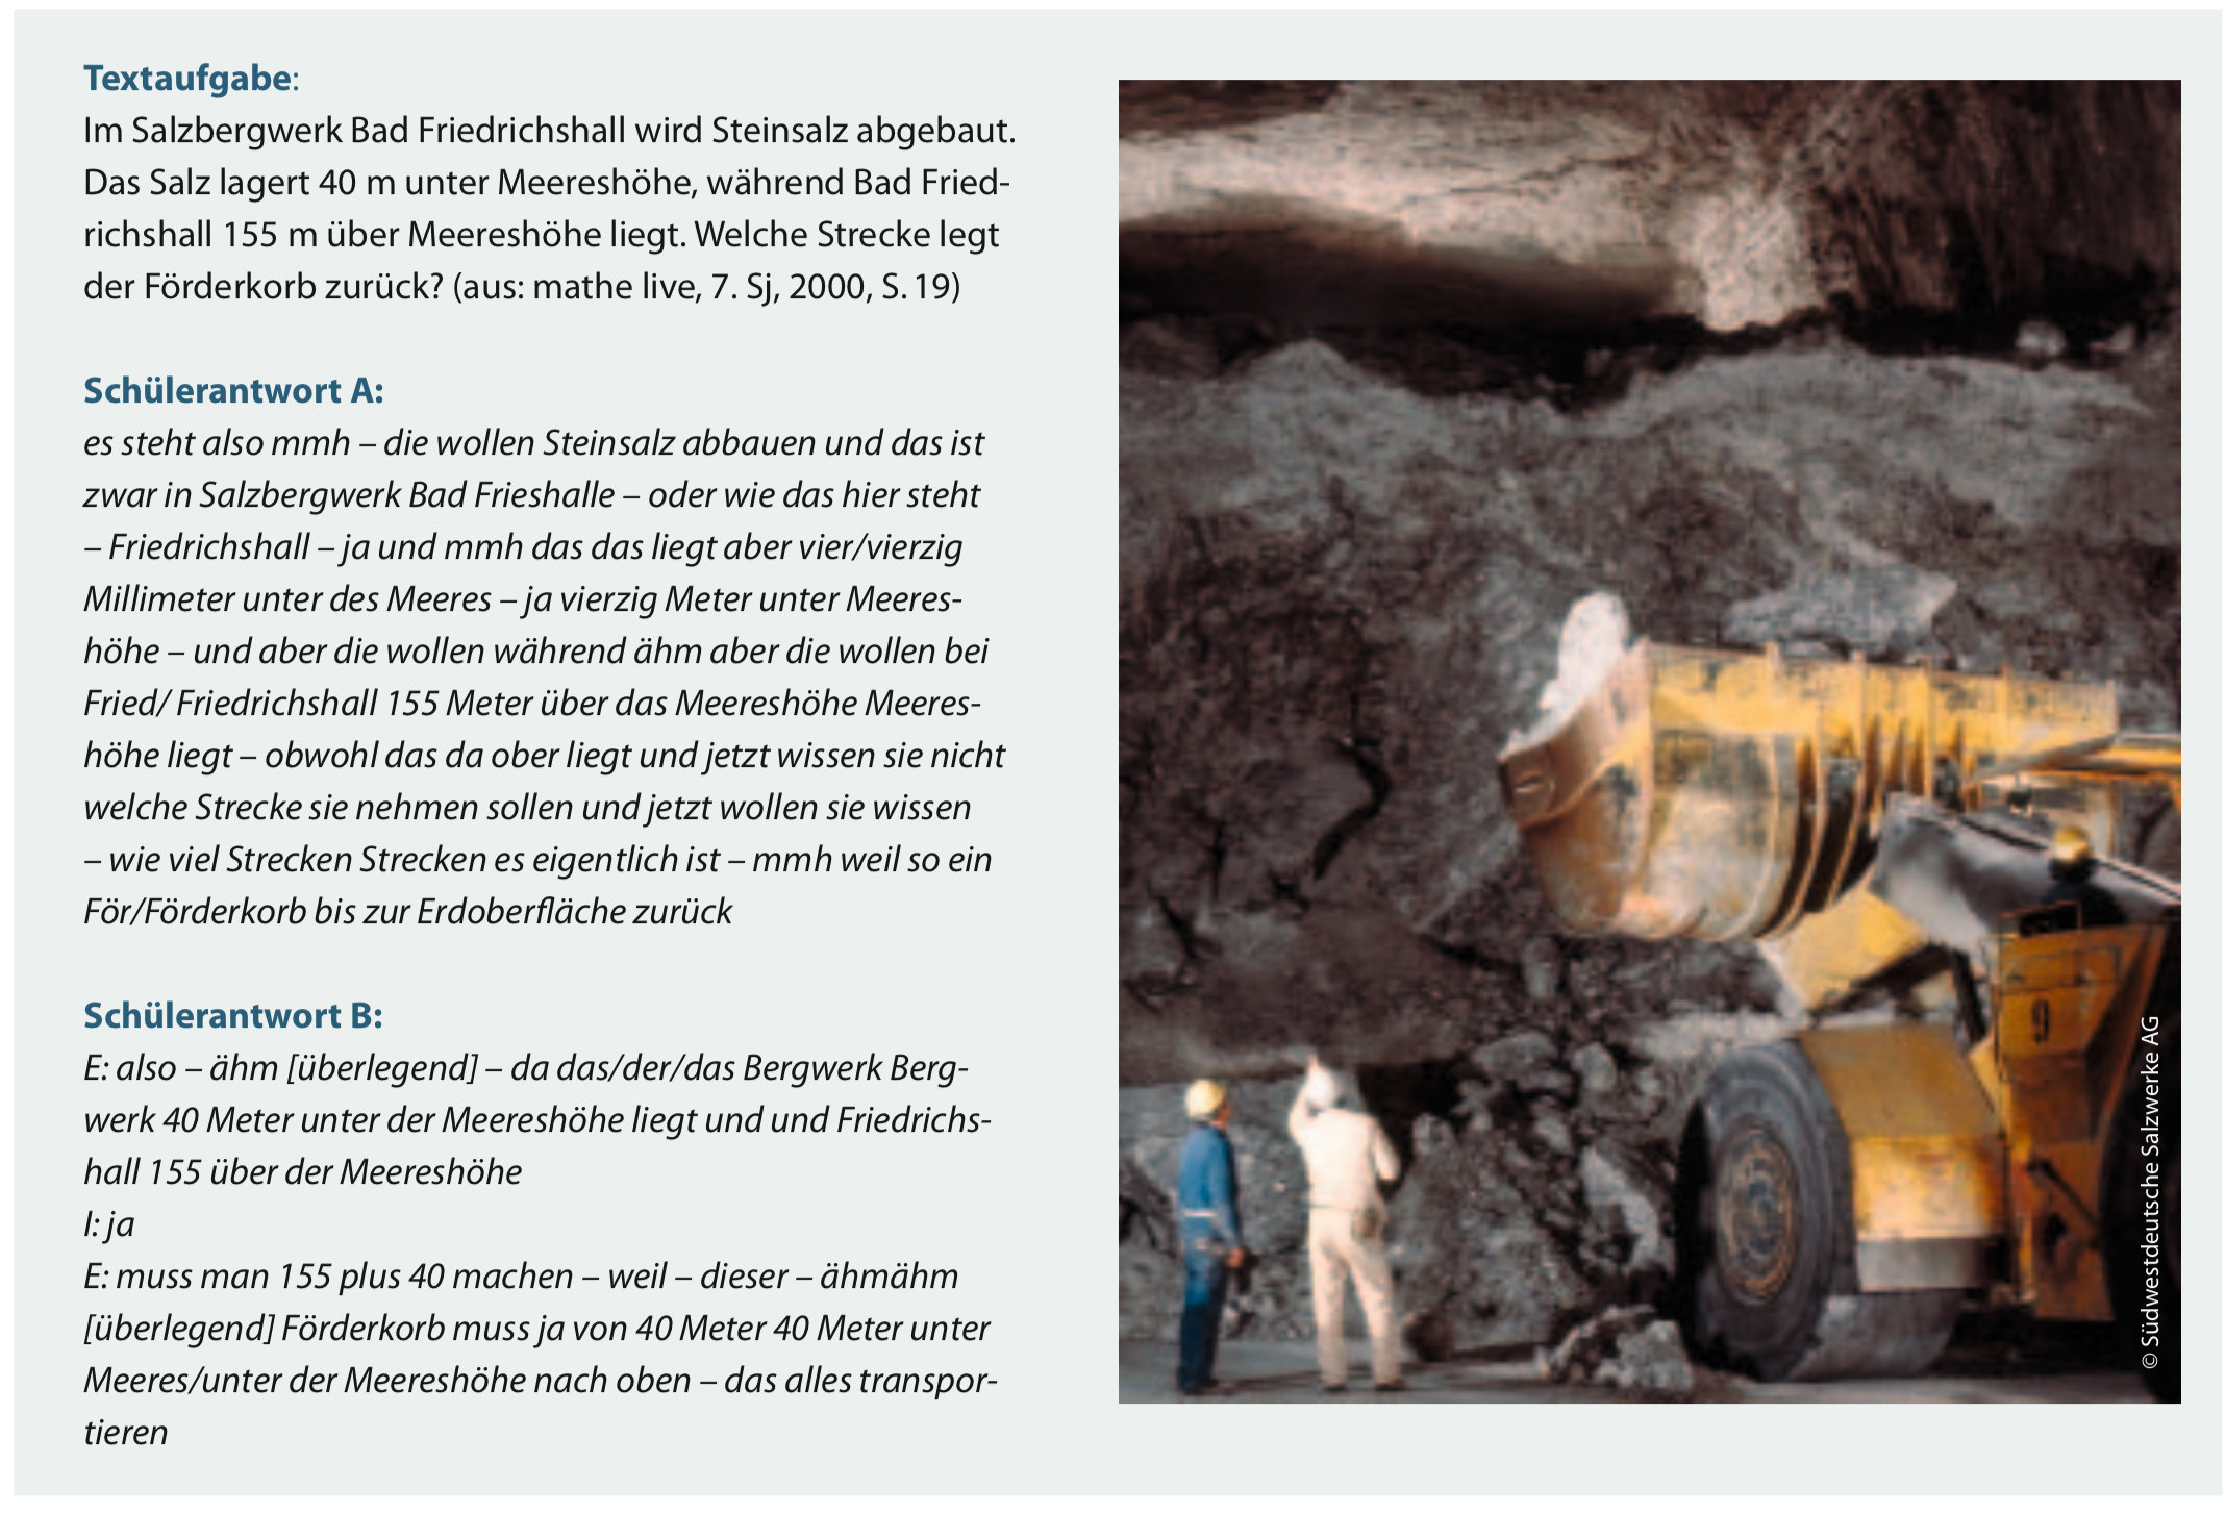
\includegraphics[height=0.68\textheight]{graphics/feilke}
\end{frame}

\begin{frame}
  {Sprachbetrachtung und Literatur im Deutsch-Abitur I}
  \pause
  Sprachlich-grammatische Betrachtung zur Literatur in Abiturarbeiten\\
  (Häcker 2009).\\[\baselineskip]
  \pause
  \centering
  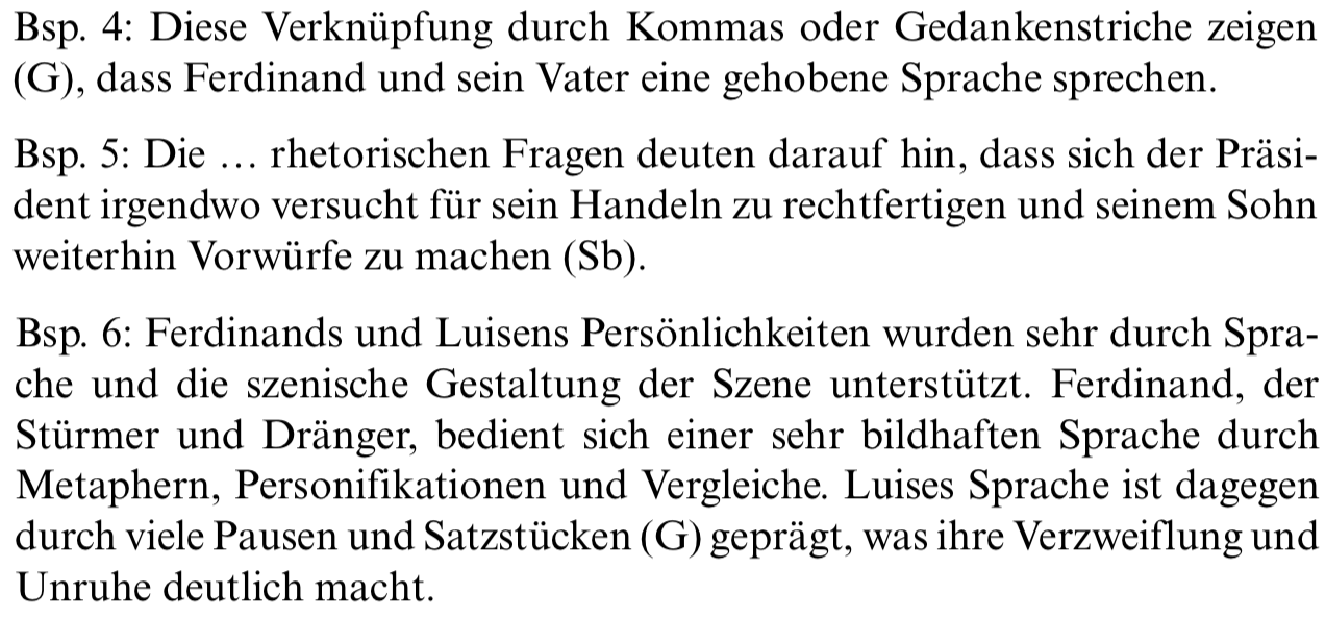
\includegraphics[height=0.5\textheight]{graphics/haecker1}
\end{frame}

\begin{frame}
  {Sprachbetrachtung und Literatur im Deutsch-Abitur II}
  Sprachlich-grammatische Betrachtung zur Literatur in Abiturarbeiten\\
  (Häcker 2009).\\[\baselineskip]
  \centering
  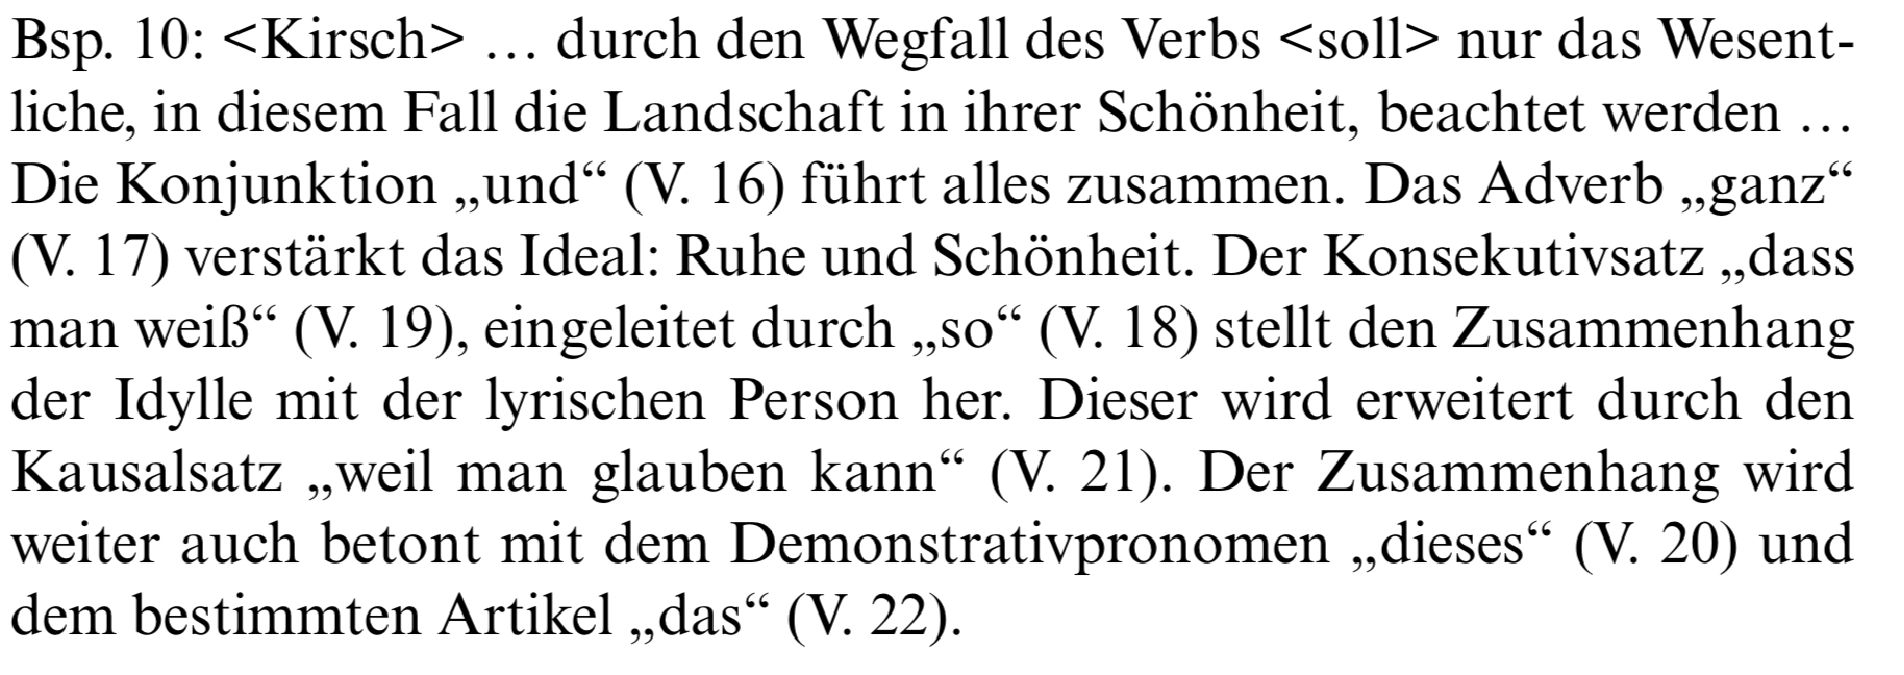
\includegraphics[height=0.4\textheight]{graphics/haecker2}
\end{frame}

\begin{frame}
  {Bildungssprache}
  \pause
  \alert{\textit{Der Deutschunterricht führt zu einem kompletten Umbau\\
  der Grammatik des Kindes.}} (nach Bredel\slash Eisenberg)\\[\baselineskip]
  \pause
  \begin{itemize}[<+->]
    \item Anforderungen:
    \begin{itemize}[<+->]
      \item Darstellung komplexer Sachverhalte
      \item \dots und nicht-faktischer (z.\,B.\ hypothetischer) Sachverhalte
      \item Intensionalität
      \item Registerbewusstsein
    \end{itemize}
        \vspace{\baselineskip}
      \item Eigenschaften:
    \begin{itemize}[<+->]
      \item dekontextualisiert
      \item schriftorientiert
      \item normorientiert
    \end{itemize}
        \vspace{\baselineskip}
      \item \alert{Das alles ist verknüpft mit spezifischen grammatischen Formen!}
  \end{itemize}
\end{frame}

\begin{frame}
  {Sprachbetrachtung}
  \pause
  \begin{itemize}[<+->]
    \item Bildungssprache $\Leftrightarrow$ Sprachbetrachtung
      \vspace{\baselineskip}
    \item Bewusstsein über richtige und angemessene Form
      \vspace{\baselineskip}
    \item explizite Sprachbetrachtung im Alltag:
      \begin{itemize}[<+->]
        \item Selbst- oder Fremdkorrektur
        \item Suche nach dem richtigen Ausdruck
        \item Orthographie optimieren
        \item Texte optimieren
        \item Begriffe definieren
        \item Grammatikalität beurteilen
      \end{itemize}
  \end{itemize}
\end{frame}

\begin{frame}
  {Die Ausgangsbasis: vorliterate Kinder und Sprachbetrachtung}
  \pause
  Klassische Studien nach Bredel (2013), Bredel et al. (2017) (s.\ EGBD3: 57--58)\\
  (Beispiele hier vereinfacht\slash dem Effekt nach neu konstruiert)\\[\baselineskip]
  \pause
  \begin{itemize}[<+->]
    \item \alert{bedeutungsbezogene} bzw.\ \alert{holistische} Betrachtung
    \item \textit{Welches Wort ist länger: Haus oder Streichholzschächtelchen?} --- \textit{Haus.}
    \item Assoziationen zu Substantiven wie \textit{Bett}: \alert{Ereignisse} \textit{schlafen gehen} usw.\\
      Erwachsene: \alert{Substantive} für andere Möbel usw.
    \item \textit{Warum heißt der Geburtstag  "`Geburtstag"'?} ---\\
      \textit{"`Weil es Geschenke und Kuchen gibt."'}
    \item \textit{Wieviele Wörter in "`Im alten Haus lebt eine junge Frau."'} --- \textit{Zwei.}
    \item \textit{Wieviele Wörter in "`Alex hat sieben Schwestern."'} --- \textit{Sieben.}
      \vspace{\baselineskip}
    \item Erfolgreich: \textit{Benenne das letzte Wort des Satzes.}
    \item[$\Rightarrow$] Die mentale Grammatik basiert auf Wörtern,\\
      der sprachbetrachtende Zugriff allerdings noch nicht!
  \end{itemize}
\end{frame}

\begin{frame}
  {Schulunterricht}
  \begin{itemize}[<+->]
    \item \alert{systematisch}
      \begin{itemize}
        \item in knapper Zeit das Ganze im Blick
      \end{itemize}
      \vspace{\baselineskip}
    \item funktional im Sinn von \alert{Form-Funktion-Beziehung}
      \begin{itemize}
        \item Formen systematisieren
        \item erst dann auf Funktionen beziehen
      \end{itemize}
      \vspace{\baselineskip}
    \item \alert{induktiv}
      \begin{itemize}
        \item keine rein deduktive Anwendung vorgegebener Begriffe
        \item Erkenntnisprozesse über sprachliche Formen und Funktionen
        \item \alert{\textit{Grammatik machen}} (Eisenberg)
      \end{itemize}
  \end{itemize}
\end{frame}

\begin{frame}
  {Aufgaben von Lehrpersonen}
  \pause
  \alert{\textit{Lehrkräften wird die Sprache der Lernenden anvertraut.}} (nach Eisenberg)\\[\baselineskip]
  \pause
  \begin{itemize}[<+->]
    \item Unterrichten der Schrift, Orthographie und Schreibung
    \item Unterweisung in Bildungssprache\slash Sprachbetrachtung
    \item Erkennen und \alert{Einordnen} von \alert{sprachlichen Defiziten}
    \item Erkennen von \alert{Interferenz mit Dialekt bzw.\ anderen Erstsprachen}
    \item \alert{Bewerten} von sprachlichen Leistungen
    \item \alert{Erklären} der Bewertung (auch gegenüber Eltern)
      \vspace{\baselineskip}
    \item[$\Rightarrow$] Anforderung: vertieftes Wissen über Sprache, vor allem Grammatik
    \item[$\Rightarrow$] Methode der sprachlichen Analyse über Faktenwissen hinaus
    \item[$\Rightarrow$] \rot{Die Grammatik für Studierende des Lehramts ist eine völlig andere\\
      als die, die sie später an Schulkinder und Jugendliche vermitteln!}
  \end{itemize}
\end{frame}

\begin{frame}
  {"`Wozu brauchen wir das denn?"'}
  \pause
  \begin{itemize}[<+->]
    \item beantwortet
    \item Linguistik und Fachdidaktik: keine praktische Anleitungen\\
      für erfolgreiche Schulstundenkonzepte
    \item Grundausbildung im \alert{Umgang mit Sprache} (Linguistik)\\
      und zum \alert{richtigen Handeln im Unterricht} (Fachdidaktik; nach Bredel)
      \vspace{\baselineskip}
    \item Minimalforderung: \alert{Examinierte Lehrkräfte müssen die\\
      Aufgaben für die späteren Lernenden selber lösen und einordnen können.}
    \item \alert{Bis nächste Woche: Bitte schauen Sie sich den Fragebogen\\
      aus Schäfer \& Sayatz (2017) an (siehe Blackboard).}
  \end{itemize}
\end{frame}



  \let\subsection\section\let\section\woopsi
  \section{Phonetik}
  \let\woopsi\section\let\section\subsection\let\subsection\subsubsection
  
\section{Rückblick}

\begin{frame}
  {Erinnerung an letzte Woche: Grammatik}
  \pause
  \begin{itemize}[<+->]
    \item unbewusste Verarbeitung → Akzeptabilität
    \item Gesetzmäßigkeiten = Regularitäten
    \item \alert{System} von Gesetzmäßigkeiten
    \item \alert{definiertes} System → Grammatikalität
    \item \alert{Kern}: Klassen\slash Regularitäten mit hoher Typenfrequenz\\
      Peripherie: niedrige Typenfrequenz
    \item Norm = Beschreibung des Grundkonsenses
  \end{itemize}
\end{frame}

\begin{frame}
  {Erinnerung an letzte Woche: Didaktik}
  \pause
  \begin{itemize}[<+->]
    \item Ziel des Deutschunterrichts: \alert{Bildungssprache}
    \item Bildungssprache + Schriftlichkeit + Norm
    \item Sprachbetrachtung im Alltag
    \item Sprachbetrachtung als Lehrkonzept
    \item Unterricht: \alert{systematisch}, \alert{Form-Funktion}, \alert{induktiv}
    \vspace{\baselineskip}
  \item \rot{Die Grammatik für Studierende des Lehramts ist eine völlig andere\\
      als die, die sie später an Schulkinder und Jugendliche vermitteln!}
  \end{itemize}
\end{frame}

\begin{frame}
  {Der Fragebogen}
  \pause
  \centering
  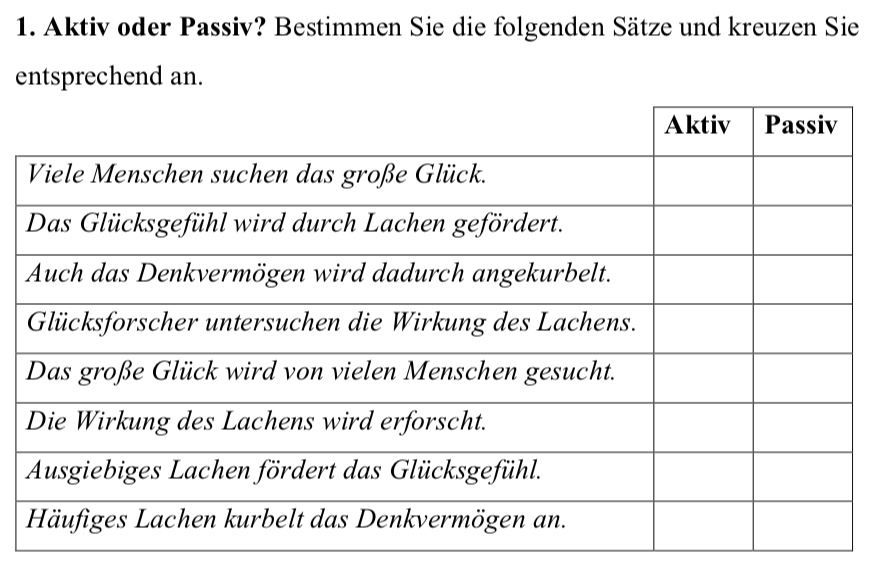
\includegraphics[width=0.75\textwidth]{\GRAPHPATH/01}
\end{frame}

\begin{frame}
  {Der Fragebogen}
  \centering
  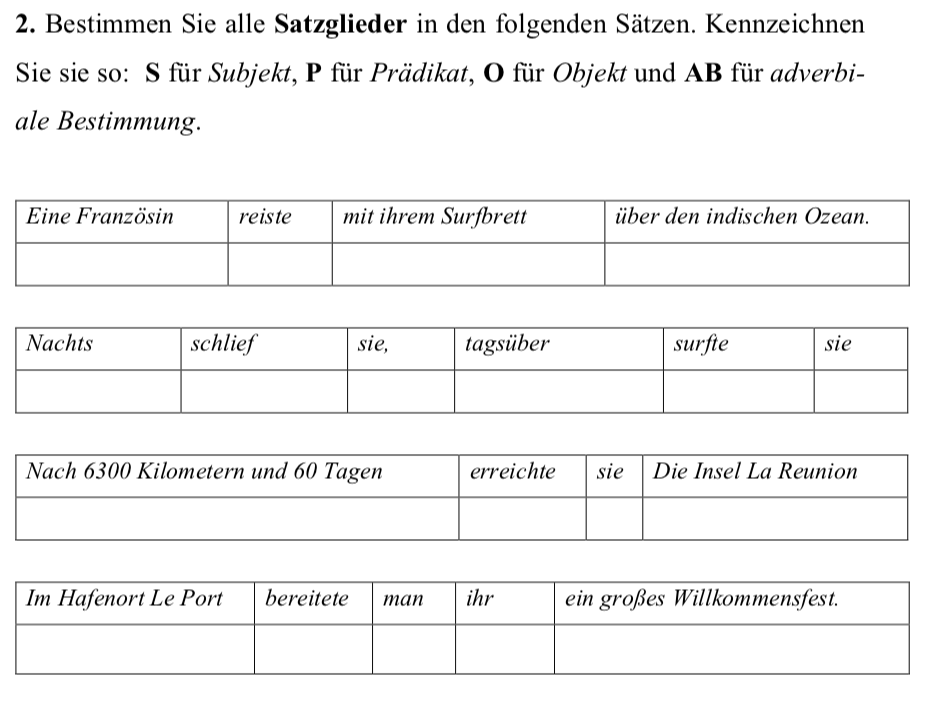
\includegraphics[width=0.75\textwidth]{\GRAPHPATH/02}
\end{frame}

\begin{frame}
  {Der Fragebogen}
  \centering
  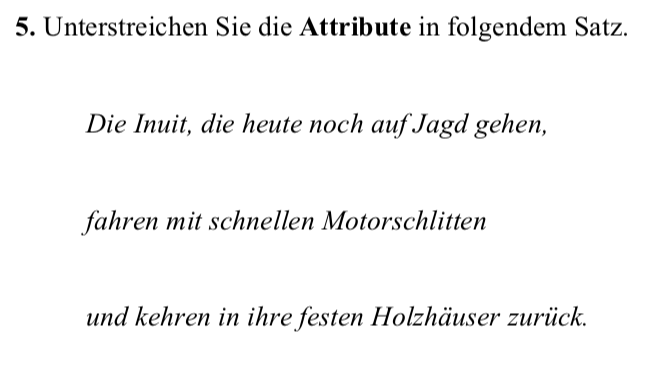
\includegraphics[width=0.75\textwidth]{\GRAPHPATH/03}
\end{frame}

\begin{frame}
  {Der Fragebogen}
  \centering
  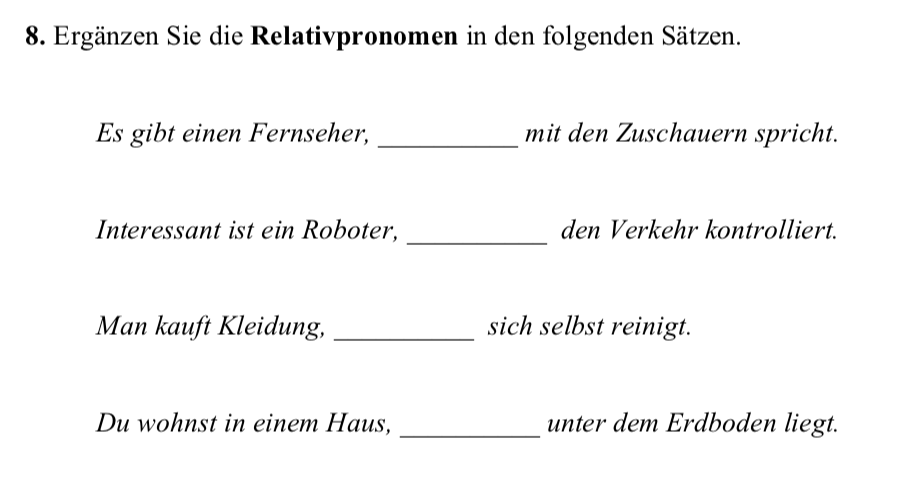
\includegraphics[width=0.75\textwidth]{\GRAPHPATH/04}
\end{frame}

\begin{frame}
  {Auswertung}
  \pause
  \centering
  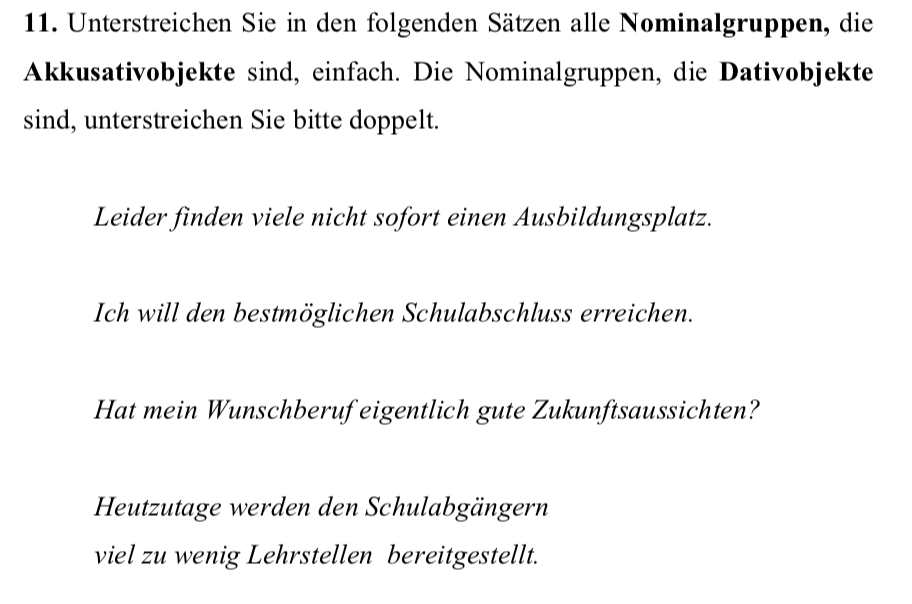
\includegraphics[width=0.75\textwidth]{\GRAPHPATH/05}
\end{frame}

\begin{frame}
  {Auswertung}
  \centering
  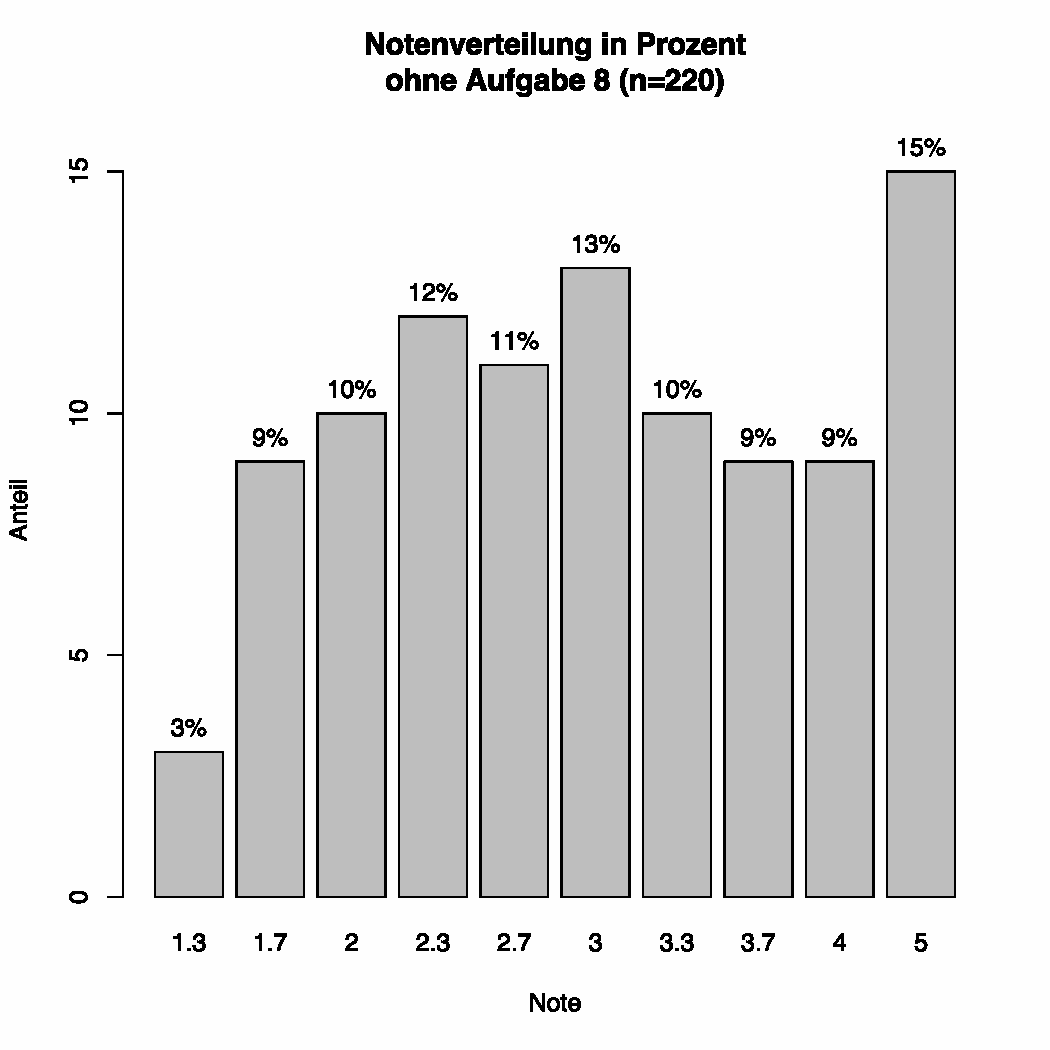
\includegraphics[width=0.6\textwidth]{\GRAPHPATH/notenspiegel}
\end{frame}

\begin{frame}
  {Auswertung}
  \centering
  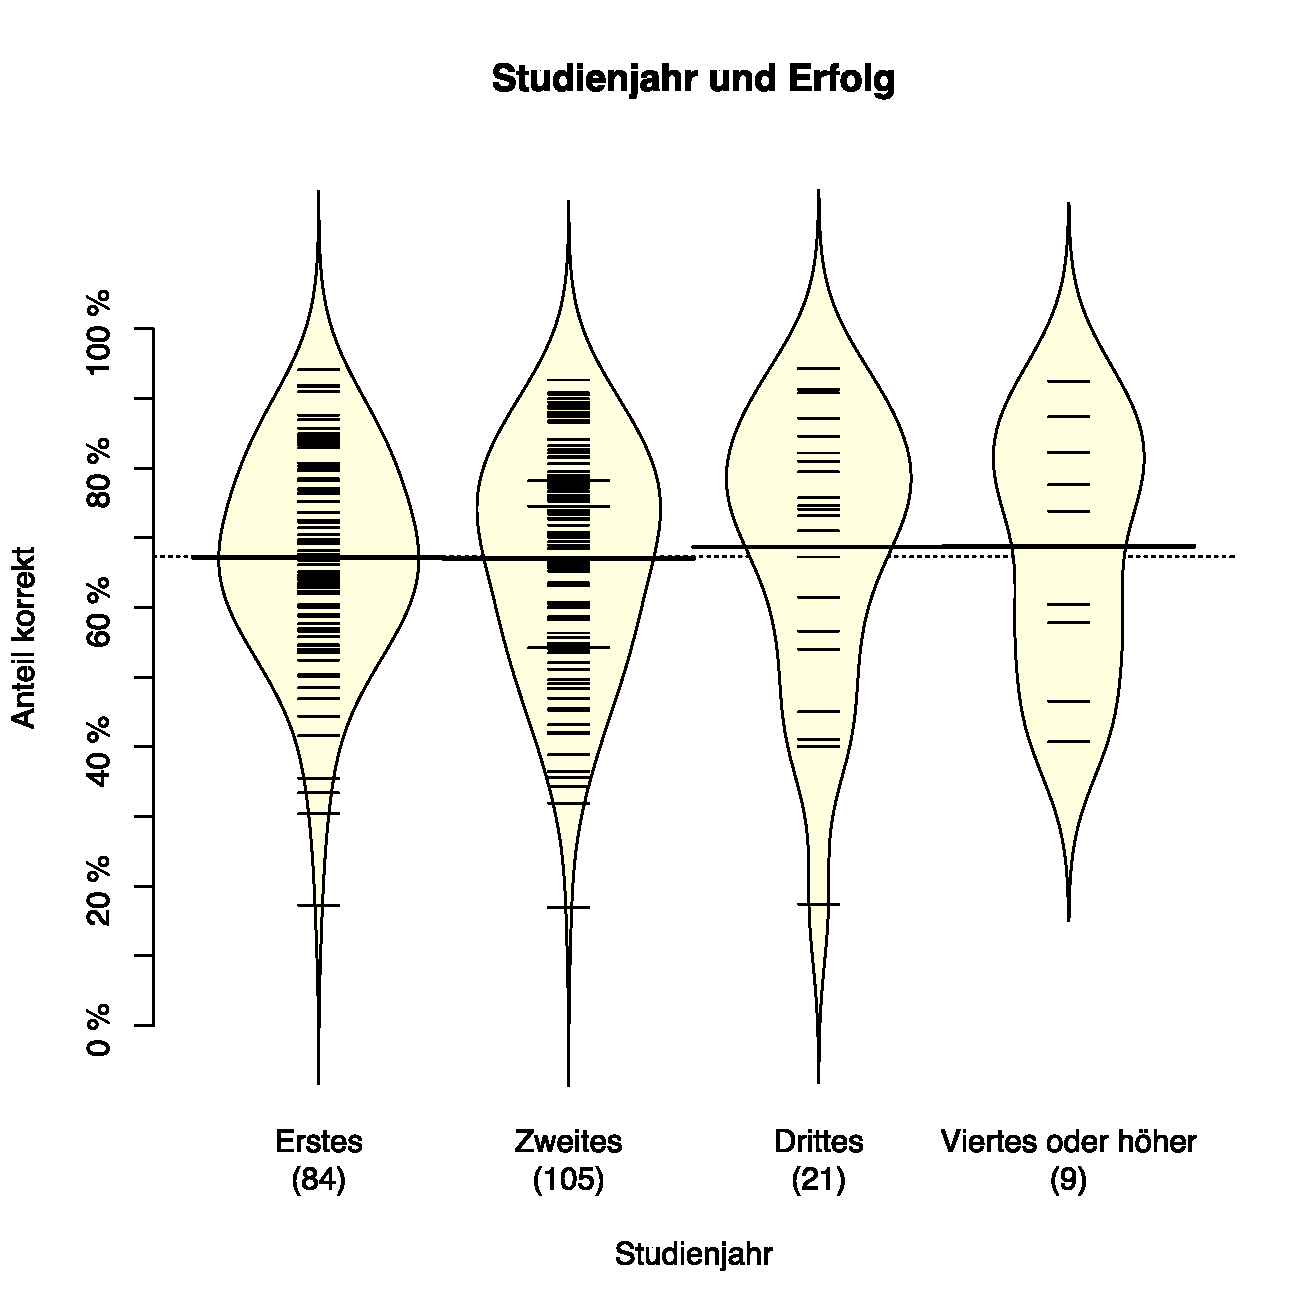
\includegraphics[width=0.6\textwidth]{\GRAPHPATH/semester}
\end{frame}

\begin{frame}
  {Auswertung}
  \centering
  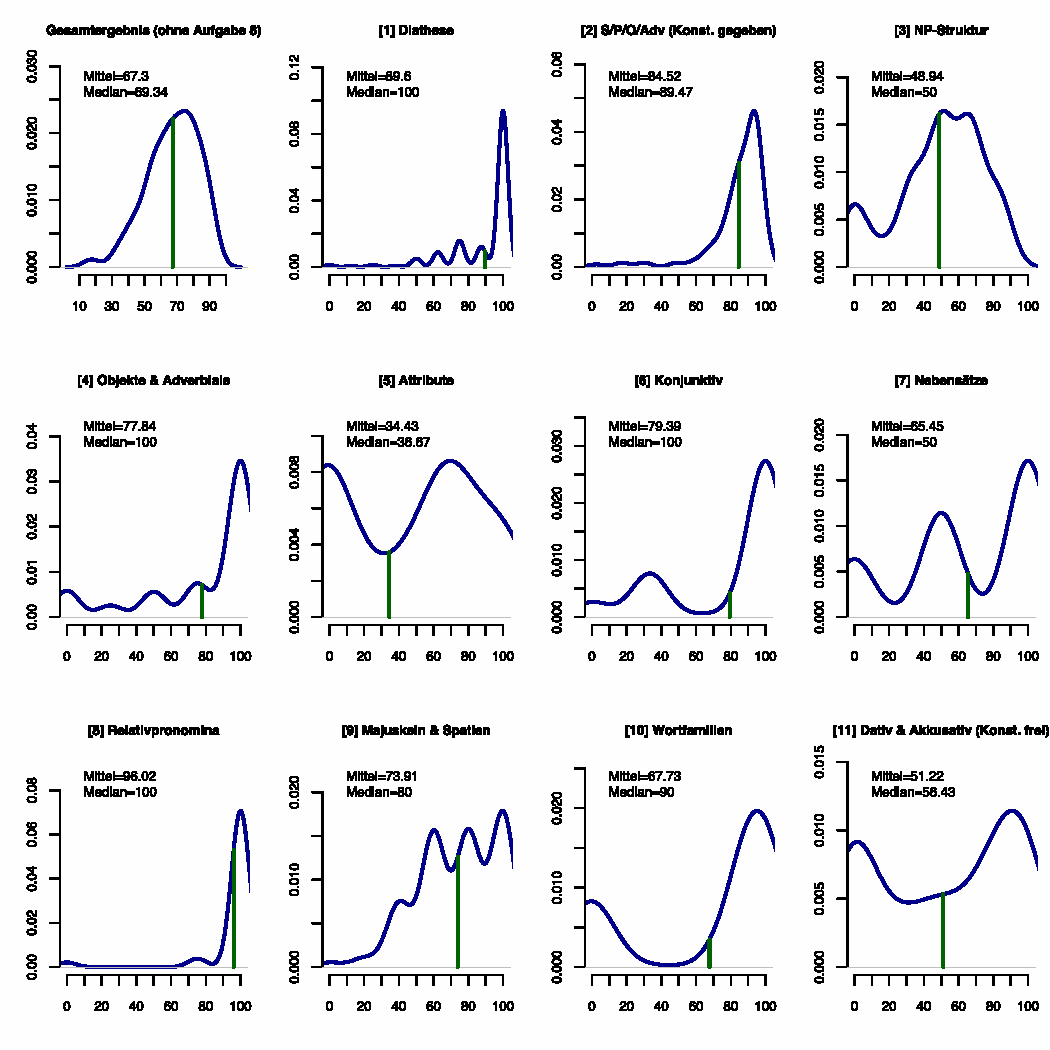
\includegraphics[width=0.6\textwidth]{\GRAPHPATH/prozentverteilung}
\end{frame}

\begin{frame}
  {Wichtige Bücher für das gesamte Studium}
  \pause
  \begin{itemize}[<+->]
    \item Grammatik\slash Linguistik:
      \begin{itemize}[<+->]
        \item \alert{\citet{Eisenberg2013a}}
        \item \alert{\citet{Eisenberg2013b}}
        \item \citet{Mueller2018} (Grammatiktheorie)
      \end{itemize}
    \vspace{\baselineskip}
    \item Linguistisch orientierte Fachdidaktik:
      \begin{itemize}[<+->]
        \item \alert{\citet{Menzel2017}}, dazu \citet{EisenbergMenzel1995}
        \item \alert{\citet{Bredel2013}}
        \item \citet{BredelEa2017} (insbesondere Grundschule)
        \item \citet{BredelPieper2015}
      \end{itemize}
  \end{itemize}
\end{frame}

\section{Phonetik}

\begin{frame}
  {Übersicht}
  \pause
  \begin{itemize}[<+->]
    \item Was ist \alert{Phonetik}?
    \item Was hat Phonetik mit \alert{Bildungssprache} zu tun?
    \item Welche \alert{Organe} sind an der Artikulation beteiligt?
    \item \alert{Wie} werden Vokale und Konsonanten artikuliert?
    \item \alert{Wo} werden Vokale und Konsonanten artikuliert?
    \item Welche Konsonanten und Vokale gibt es im \alert{Standard}?
  \end{itemize}
\end{frame}

\begin{frame}
  {Medien}
  \pause
  \begin{itemize}[<+->]
    \item akustisch
    \item artefaktisch (\zB Schrift)
    \item gestisch
    \vspace{\baselineskip}
  \item Beziehungen?
  \item \textit{Das schreibt man wie man es spricht?}
  \end{itemize}
\end{frame}

\begin{frame}
  {Methode und Ziele}
  \pause
  \begin{itemize}[<+->]
    \item \alert{artikulatorische} Phonetik: Produktion
    \item \alert{perzeptorische} Phonetik: Wahrnehmung
    \item \alert{akustische} Phonetik: physikalische Gestalt
    \vspace{\baselineskip}
  \item Warum \rot{artikulatorisch}?
    \begin{itemize}[<+->]
      \item Transkriptionsalphabete
      \item Grundlage der Phonologie
      \item Grundlage Sprecherziehung i.\,w.\,S.
      \item weitgehend apparatefrei möglich
      \item weitgehend experimentfrei möglich
    \end{itemize}
    \vspace{\baselineskip}
  \item Empfohlene Literatur: \citet{RuesEa2009}
  \end{itemize}
\end{frame}

\begin{frame}
  {Phonetik und Bildungssprache}
  \pause
  \begin{itemize}[<+->]
    \item phonetische Normbeherrschung: Primärmerkmal
    \vspace{0.5\baselineskip}
    \item Prestige
      \begin{itemize}[<+->]
        \item William Labov 1966: (nicht-)rhotische Varietäten des Englischen
        \item drei Kaufhäuser in NYC, drei "`Schichten"'
        \item \textit{r} nach Vokal als \alert{Schichtindikator}
        \item situative Anpassung
      \end{itemize}
  \item Anke Engelkes \textit{Deutschkurs für türkische Mitbürger*innen}
    \vspace{0.5\baselineskip}
    \item \alert{Dialekte, Soziolekte, Kiezsprachen erhalten!}
    \item \rot{Standard lehren!}
    \item zukünftige Lehrpersonen
      \begin{itemize}
        \item Phonetik $\not\subset$ Schulstoff
        \item \rot{Erkennen von Ausspracheproblemen in der Norm}
        \item \alert{richtige Reaktion nur mit phonetischem Wissen}
      \end{itemize}
  \end{itemize}
\end{frame}

\begin{frame}
  {Artikulationsorgane}
  \pause
  \centering
  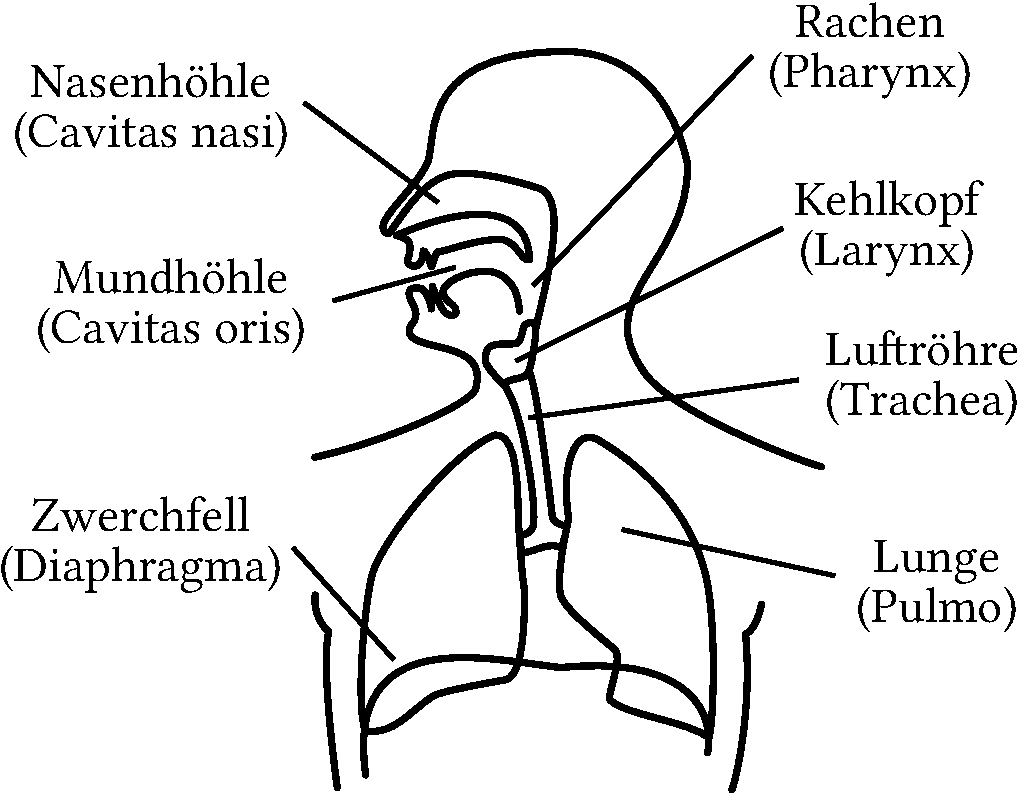
\includegraphics[height=0.7\textheight]{\GRAPHPATH/ueberblick}
\end{frame}

\begin{frame}
  {Mundraum}
  \pause
  \centering
  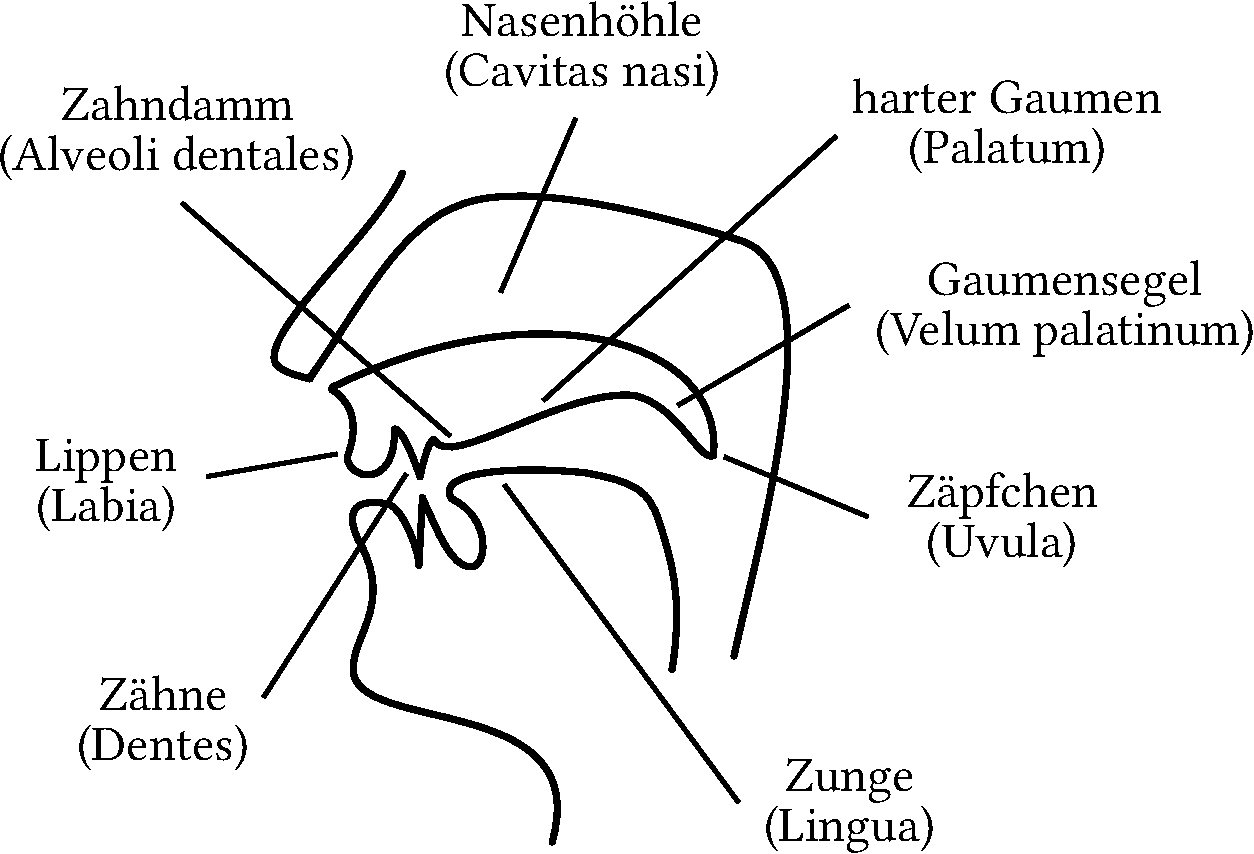
\includegraphics[height=0.7\textheight]{\GRAPHPATH/mundraum}
\end{frame}

\begin{frame}
  {Artikulationen: Konsonanten}
  \pause
    \begin{exe}
      \ex \alert{P}ole, \alert{B}ohle; \alert{T}ank, \alert{D}ank; \alert{g}ilt, \alert{k}illt
      \pause
      \ex \alert{F}ee, \alert{w}eh; hei\alert{ß}er, hei\alert{s}er; schli\alert{ch}, \alert{J}ubel; Ba\alert{ch}, \alert{R}une
      \pause
      \ex \alert{Pf}anne; \alert{Z}irkus; Ma\alert{tsch}
      \pause
      \ex \alert{M}us; \alert{N}uss; Go\alert{ng}
    \end{exe}
    \pause
    \Large
    \begin{itemize}
      \item \alert{Stimmhaftigkeit}
    \end{itemize}
\end{frame}


\begin{frame}
  {Artikulationen: Konsonanten}
  \pause
  \begin{exe}
    \ex \alert{P}a\alert{pp}e, \alert{b}e\alert{b}auen
    \pause
    \ex \alert{T}in\alert{t}e, \alert{d}ul\alert{d}en
    \pause
    \ex \alert{K}na\alert{ck}, \alert{g}e\alert{g}en
    \pause
    \ex Cha\alert{?}ot (Chaos)
    \ex \alert{?}Anfang, \alert{?}über, \alert{?}ohne, \alert{?}Uhr, \dots
  \end{exe}
    \pause
    \Large
    \begin{itemize}
      \item \alert{Plosive}
    \end{itemize}
\end{frame}


\begin{frame}
  {Artikulationen: Konsonanten}
  \pause
  \begin{exe}
    \ex \alert{f}ün\alert{f}, \alert{w}ehe
    \pause
    \ex Bu\alert{s}, \alert{S}ahne
    \pause
    \ex Bä\alert{ch}e, \alert{J}och
    \pause
    \ex Ba\alert{ch}e, \alert{R}asen
  \end{exe}
    \pause
    \Large
    \begin{itemize}
      \item \alert{Frikative}
    \end{itemize}
\end{frame}

\begin{frame}
  {Artikulationen: Konsonanten}
  \pause
  \begin{exe}
    \ex \alert{Pf}anne, To\alert{pf} 
    \pause
    \ex \alert{Z}ange, Schli\alert{tz}
    \pause
    \ex Ma\alert{tsch} (\alert{Ch}ips)
    \pause
    \ex (\alert{Dsch}ungel)
  \end{exe}
    \pause
    \Large
    \begin{itemize}
      \item \alert{Affrikaten}
    \end{itemize}
\end{frame}

\begin{frame}
  {Artikulationen: Konsonanten}
  \pause
  \begin{exe}
    \ex \alert{L}icht, Ba\alert{ll}
  \end{exe}
    \pause
    \Large
    \begin{itemize}
      \item \alert{Approximanten}
    \end{itemize}
    \Zeile
  \pause
  \begin{exe}
    \ex \alert{M}aus, Bau\alert{m}
    \pause
    \ex \alert{N}ase, Ki\alert{nn}
    \pause
    \ex Ri\alert{ng}
  \end{exe}
    \pause
    \Large
    \begin{itemize}
      \item \alert{Nasale}
    \end{itemize}
\end{frame}


\begin{frame}
  {Artikulationen: Vokale}
  \pause
  \begin{exe}
    \ex T\alert{ie}r, T\alert{ü}r; g\alert{u}t
    \pause
    \ex w\alert{e}nig, Fl\alert{ö}te; H\alert{o}se
    \pause
    \ex k\alert{ä}me
    \pause
    \ex B\alert{a}d
    \Zeile
    \pause
    \ex K\alert{i}nd, M\alert{ü}ndel; B\alert{u}s
    \pause
    \ex k\alert{ä}mme, k\alert{ö}nnen; Sch\alert{o}ck
    \pause
    \ex T\alert{a}nne
    \Zeile
    \pause
    \ex s\alert{ei}, Pf\alert{au}, H\alert{eu}
    \Zeile
    \pause
    \ex Tüt\alert{e}, b\alert{e}sonders, Eh\alert{e}, \dots
  \end{exe}
\end{frame}


\begin{frame}
  {Artikulationsarten}
  \pause
  \resizebox{\textwidth}{!}{
  \begin{tikzpicture}[every text node part/.style={align=center}]
    \node (UeVok) at (0,0)  {\textbf{Vokale}\\(prototypisch\\silbisch)};
    \node (UeApr) at (2.5,2)  {Approximanten};
    \node (UeNas) at (5,2)  {Nasale};
    \node (UeFri) at (7.5,2)  {Frikative};
    \node (UeAfr) at (10,2) {Affrikaten};
    \node (UePlo) at (12.5,2)  {Plosive};

    \node (UeSon) at (0,4) {\textbf{Sonoranten}\\(Klanglaute)};
    \node (UeObs) at (12.5,4) {\textbf{Obstruenten}\\(Geräuschlaute)};

    \node (UeKon) at (12.5,0) {\textbf{Konsonanten}\\(prototypisch\\nicht silbisch)};

    \draw (UeSon) to (UeVok);
    \draw [bend left] (UeSon) to (UeApr);
    \draw [bend left] (UeSon) to (UeNas);

    \draw (UeObs) to (UePlo);
    \draw [bend right] (UeObs) to (UeFri);
    \draw [bend right] (UeObs) to (UeAfr);

    \draw [bend right] (UeApr) to (UeKon);
    \draw [bend right] (UeNas) to (UeKon);
    \draw (UePlo) to (UeKon);
    \draw [bend right] (UeFri) to (UeKon);
    \draw [bend right] (UeAfr) to (UeKon);
  \end{tikzpicture}}
\end{frame}

\begin{frame}
  {Artikulationsorte (Konsonanten)}
  \pause
  \begin{exe}
    \ex \alert{P}a\alert{pp}e, \alert{B}irne, \alert{M}ulch
    \pause
    \ex \alert{F}ahne, \alert{W}itz, \alert{Pf}usch
    \pause
    \ex \alert{T}raum, \alert{d}ort, Mi\alert{s}t, \alert{s}ing, \alert{Z}under, \alert{L}uft, \alert{n}och
    \pause
    \ex Bu\alert{sch}, \alert{Tsch}echisch
    \pause
    \ex schle\alert{ch}t, \alert{J}unge
    \pause
    \ex Ro\alert{ck}, \alert{G}abe, Kli\alert{ng}e
    \pause
    \ex wa\alert{ch}, \alert{r}ütteln
    \pause
    \ex \alert{?}offen, \alert{h}och
  \end{exe}
\end{frame}


\begin{frame}
  {Welche Konsonanten gibt es?}
  \centering
  \resizebox{0.7\textwidth}{!}{
  \begin{tabular}{rccccccccc}
    \toprule
    \multicolumn{1}{c}{} & \Sw{\textbf{bilabial}} & \Sw{\textbf{labiodental}} & \Sw{\textbf{alveolar}} & \Sw{\textbf{palatoalveolar}} & \Sw{\textbf{palatal}} & \Sw{\textbf{velar}} & \Sw{\textbf{uvular}} & \Sw{\textbf{laryngal}} \\
    \midrule
    \textbf{stl.\ Plosiv} & p &  & t &  &  & k &  & ʔ \\
    \textbf{sth.\ Plosiv} & b &  & d &  &  & g &  &  \\
    \textbf{stl.\ Frikativ} &  & f & s & ʃ & ç &  & χ & h \\
    \textbf{sth.\ Frikativ} &  & v & z &  & ʝ &  & ʁ &  \\
    \textbf{stl.\ Affrikate} &  & p͡f & t͡s & t͡ʃ &  &  &  &  \\
    \textbf{lateraler Approximant} &  &  & l &  &  &  &  &  \\
    \textbf{Nasal} & m &  & n &  &  & ŋ &  &  \\
    \bottomrule
  \end{tabular}  
  }
\end{frame}


\begin{frame}[fragile]
  {Welche Vokale gibt es?}
  \begin{center}
  \resizebox{0.6\textwidth}{!}{
  \begin{tikzpicture}[scale=2.5,baseline=default]
    \large
    \tikzset{
      vowel/.style={fill=white, anchor=mid, text depth=0ex, text height=1ex},
      dot/.style={circle,fill=black,minimum size=0.4ex,inner sep=0pt,outer sep=-1pt},
    }

    \coordinate (hf) at (0,2); % high front
    \coordinate (hb) at (2,2); % high back
    \coordinate (lf) at (1,0); % low front
    \coordinate (lb) at (2,0); % low back
    \def\V(#1,#2){barycentric cs:hf={(3-#1)*(2-#2)},hb={(3-#1)*#2},lf={#1*(2-#2)},lb={#1*#2}}

    % Chart key (vorne -- hinten).
    \draw [{Latex[round]}-] (\V (-.25,0))   -- (\V (-.25,.5)) node [above left] {\footnotesize vorne};
    \draw [-{Latex[round]}] (\V (-.25,1.5)) -- (\V (-.25,2))  node [above left] {\footnotesize hinten};
    \path (\V (-.25,1)) node[above] {\footnotesize zentral};

    % Chart key (hoch--tief).
    \draw [{Latex[round]}-] (\V (0,-.25)) -- +(270:.5cm)  node [above right,rotate=90] (vokaltrapez1) {\footnotesize hoch};
    \draw [{Latex[round]}-] (\V (3,-2.5)) -- +(270:-.5cm) node [above left,rotate=90] (vokaltrapez2) {\footnotesize tief};
    \path (\V (1.5,-1)) node[above,rotate=90] {\footnotesize mittel};

    % Grid. 
    \draw [gray, thick] (\V(0,0)) -- (\V(0,2));
    \draw [gray, thick] (\V(1,0)) -- (\V(1,2));
    \draw [gray, thick] (\V(2,0)) -- (\V(2,2));
    \draw [gray, thick] (\V(3,0)) -- (\V(3,2));
    \draw [gray, thick] (\V(0,0)) -- (\V(3,0));
    \draw [gray, thick] (\V(0,1)) -- (\V(3,1));
    \draw [gray, thick] (\V(0,2)) -- (\V(3,2));

    % Unrounded-rounded pairs.
    \path (\V(0,0))     node[vowel, left]     {i} node[vowel, right] (y) {y} node[dot] {};
    \path (\V(0.5,0.5)) node[vowel, left]     {ɪ} node[vowel, right] (Y) {ʏ} node[dot] {};
    \path (\V(1,0))     node[vowel, left]     {e} node[vowel, right] (e) {ø} node[dot] {};
    \path (\V(2,0))     node[vowel, left] (E) {ɛ} node[vowel, right] (ee) {œ} node[dot] {};

    % Unpaired symbols.
    \path (\V(1.5,1))    node [vowel] (schwa)  {ə};
    \path (\V(2.5,1))    node [vowel] (schwaa) {ɐ};
    \path (\V(3,1))      node [vowel] (a)      {a};
    \path (\V (2,2))     node [vowel] (oo)     {ɔ};
    \path (\V (1,2))     node [vowel] (o)      {o};
    \path (\V (0,2))     node [vowel] (u)      {u};
    \path (\V (0.5,1.5)) node [vowel] (uu)     {ʊ};

    \path (a)  edge [-{Latex[round]}, bend right=15] (oo);
    \path (a)  edge [-{Latex[round]}, bend left=15]  (E);
    \path (oo) edge [-{Latex[round]}, bend right=15] (ee);
  \end{tikzpicture}
  }
  \end{center}
\end{frame}

\begin{frame}
  {Artikulation anschaulich}
  \vspace{2\baselineskip}
  \centering
  \Large Artikulationsfilme\dots
\end{frame}


\begin{frame}
  {Besonderheiten: Endrand-Desonorisierung}
  \pause
  \begin{exe}
    \ex\label{ex:auslautverhaertung011}
    \begin{xlist}
      \ex{\label{ex:auslautverhaertung012} weck [vɛk]}
      \ex{\label{ex:auslautverhaertung013} Weg [veːk]}
      \ex{\label{ex:auslautverhaertung014} Weges [veːgəs]}
    \end{xlist}
  \pause
    \ex\label{ex:auslautverhaertung015}
    \begin{xlist}
      \ex{\label{ex:auslautverhaertung016} bat [baːt]}
      \ex{\label{ex:auslautverhaertung017} Bad [baːt]}
      \ex{\label{ex:auslautverhaertung018} Bades [baːdəs]}
    \end{xlist}
  \pause
    \ex\label{ex:auslautverhaertung019}
    \begin{xlist}
      \ex{\label{ex:auslautverhaertung020} Flop [flɔp]}
      \ex{\label{ex:auslautverhaertung021} Lob [loːp]}
      \ex{\label{ex:auslautverhaertung022} Lobes [loːbəs]}
    \end{xlist}
  \end{exe}
\end{frame}


\begin{frame}
  {Besonderheiten: Silbische Nasale und Liquiden}
  \pause
  \begin{exe}
    \ex\label{ex:silbischenasaleundapproximanten023}
    \begin{xlist}
      \ex{laufen [la͡ɔfn̩]~\slash~[la͡ɔfən]}
      \ex{haben [habm̩]~\slash~[habən]}
      \ex{kriegen [kʁiːgŋ̩]~\slash~[kʁiːgən]}
      \ex{rotem [ʁoːtm̩]~\slash~[ʁoːtəm]}
      \ex{Bündel [bʏndl̩]~\slash~[bʏndəl]}
    \end{xlist}
  \end{exe}
\end{frame}

\begin{frame}
  {Besonderheiten: \textit{r}-Laute}
  \pause
  \begin{exe}
    \ex\label{ex:orthographischesr030}
    \begin{xlist}
      \ex{Tier [ti͡ɐ], Tür [ty͡ɐ]}
      \ex{Kirche [kɪ͡əçə], Bürde [bʏ͡ədə]}
      \ex{nur [nu͡ɐ]}
      \ex{Bursche [bʊ͡əʃə]}
      \ex{der [de͡ɐ], Stör [ʃtø͡ɐ]}
      \ex{Chor [ko͡ɐ]}
      \ex{gern [gɛ͡ən], Börse [bœ͡əzə]}
      \ex{Korn [kɔ͡ən]}
      \ex{Bar [ba͡ə]}
      \ex{knarr [kna͡ə]}
    \end{xlist}
  \end{exe}
\end{frame}


\begin{frame}[fragile]
  {Sekundäre Diphthonge}
  \begin{center}
  \resizebox{0.6\textwidth}{!}{
  \begin{tikzpicture}[scale=3,baseline=default]
    \large
    \tikzset{
    vowel/.style={fill=white, anchor=mid, text depth=0ex, text height=1ex},
    dot/.style={circle,fill=black,minimum size=0.4ex,inner sep=0pt,outer sep=-1pt},
    }

    \coordinate (hf) at (0,2); % high front
    \coordinate (hb) at (2,2); % high back
    \coordinate (lf) at (1,0); % low front
    \coordinate (lb) at (2,0); % low back
    \def\V(#1,#2){barycentric cs:hf={(3-#1)*(2-#2)},hb={(3-#1)*#2},lf={#1*(2-#2)},lb={#1*#2}}

    % Chart key (vorne -- hinten).
    \draw [{Latex[round]}-] (\V (-.25,0)) -- (\V (-.25,.5))  node [above left] {\footnotesize vorne};
    \draw [-{Latex[round]}] (\V (-.25,1.5)) -- (\V (-.25,2)) node [above left] {\footnotesize hinten};
    \path (\V (-.25,1)) node[above] {\footnotesize zentral};

    % Chart key (hoch--tief).
    \draw [{Latex[round]}-] (\V (0,-.25)) -- +(270:.5cm)  node [above right,rotate=90] (vokaltrapez1) {\footnotesize hoch};
    \draw [{Latex[round]}-] (\V (3,-2.5)) -- +(270:-.5cm) node [above left,rotate=90] (vokaltrapez2) {\footnotesize tief};
    \path (\V (1.5,-1)) node[above,rotate=90] {\footnotesize mittel};

    % Grid.
    \draw [gray, thick] (\V(0,0)) -- (\V(0,2));
    \draw [gray, thick] (\V(1,0)) -- (\V(1,2));
    \draw [gray, thick] (\V(2,0)) -- (\V(2,2));
    \draw [gray, thick] (\V(3,0)) -- (\V(3,2));
    \draw [gray, thick] (\V(0,0)) -- (\V(3,0));
    \draw [gray, thick] (\V(0,1)) -- (\V(3,1));
    \draw [gray, thick] (\V(0,2)) -- (\V(3,2));

    % Unrounded-rounded pairs.
    \path (\V(0,0))     node[vowel, left] {i} node [vowel, right] (y)  {y} node [dot] {};
    \path (\V(0.5,0.5)) node[vowel, left] {ɪ} node [vowel, right] (Y)  {ʏ} node [dot] {};
    \path (\V(1,0))     node[vowel, left] {e} node [vowel, right] (e)  {ø} node [dot] {};
    \path (\V(2,0))     node[vowel, left] {ɛ} node [vowel, right] (ee) {œ} node [dot] {};

    % Unpaired symbols.
    \path (\V(1.5,1))    node [vowel] (schwa)  {ə};
    \path (\V(2.5,1))    node [vowel] (schwaa) {ɐ};
    \path (\V(3,1))      node [vowel] (a)      {a};
    \path (\V (2,2))     node [vowel] (oo)     {ɔ};
    \path (\V (1,2))     node [vowel] (o)      {o};
    \path (\V (0,2))     node [vowel] (u)      {u};
    \path (\V (0.5,1.5)) node [vowel] (uu)     {ʊ};

    % Connections.
    \path (y) edge  [-{Latex[round]}, bend right=3]  (schwaa);
    \path (e) edge  [-{Latex[round]}, bend right=10] (schwaa);
    \path (ee) edge [-{Latex[round]}, bend left=20]  (schwa);
    \path (a) edge  [-{Latex[round]}, bend right=40] (schwa);
    \path (oo) edge [-{Latex[round]}, bend right=20] (schwa);
    \path (o) edge  [-{Latex[round]}, bend left=15]  (schwaa);
    \path (u) edge  [-{Latex[round]}, bend left=10]  (schwaa);
    
    \draw [-{Latex[round]}]             (Y)  -- (schwa);
    \draw [-{Latex[round]}, bend right] (uu) -- (schwa);
  \end{tikzpicture}
  }
  \end{center}
\end{frame}


\section{Vorschau}

\begin{frame}
  {Von der Phonetik zur Phonologie}
  \pause
  \begin{itemize}[<+->]
    \item Wiederholung\slash Übung der Phonetik
    \item Vorkommen von Segmenten: nicht alle überall
    \item System: zugrundeliegende Segmente und Prozesse
    \item Vorgriff auf die Graphematik: Buchstaben und Segmente
      \Zeile
    \item \rot{Lesen Sie bitte: Kapitel 5, S.~111--123}
    \item \alert{Wiederholen: Kapitel 4, S.~104--108}
  \end{itemize}

  \pause
  \pause
  \pause
  \pause
  \pause
\end{frame}



  
  \let\subsection\section\let\section\woopsi
  \section[Segmente]{Segmentale Phonologie}
  \let\woopsi\section\let\section\subsection\let\subsection\subsubsection
  
\section{Rückblick}

\begin{frame}
  {Erinnerung an letzte Woche: Phonetik}
  \pause
  \begin{itemize}[<+->]
    \item Artikulationsorgane
    \item Konsonanten
      \begin{itemize}
        \item Stimmton
        \item Art: Plosiv, Frikativ, Affrikate, Nasal, Approximant
      \end{itemize}
    \item Vokale:
      \begin{itemize}
        \item vorne -- hinten
        \item hoch -- tief
        \item gerundet -- ungerundet
        \item lang -- kurz
        \item Diphthonge
      \end{itemize}
    \item Sonoranten und Obstruenten
    \item r-Laute und sekundäre Diphthonge
  \end{itemize}
\end{frame}


\section{Phonologie}

\begin{frame}
  {Übersicht}
  \pause
  \begin{itemize}[<+->]
    \item \alert{Segmente} als Einheiten der Phonetik\slash Phonologie
    \item nicht alle Segmente überall: \alert{Verteilungen}
    \item Endrand-Desonorisierung, r-Vokalisierung, \textit{ich}\slash\textit{ach}-Laute usw.\\
      und \alert{Ableitung} phonetischer Formen aus lexikalischen Formen
    \item längbare, betonbare und unbetonbare Vokale
      \Zeile
    \item empfohlene Literatur: \citet{Eisenberg2013a} (Grundriss: Wort)
  \end{itemize}
\end{frame}

\begin{frame}
  {Was hat Phonologie mit Bildungs- und Normsprache zu tun?}
  \pause
  \begin{itemize}[<+->]
    \item mit Bildungssprache nicht viel
    \item mit Normsprache sehr viel
      \begin{itemize}[<+->]
        \item Viele dialektale und soziolektale Einflüsse sind\\
          phonologisch statt phonetisch.
        \item Das graphematische System ist am phonologischen orientiert.
        \item Worttrennung
      \end{itemize}
  \end{itemize}
\end{frame}

\begin{frame}
  {Segmente}
  \pause
  \begin{itemize}[<+->]
    \item Transkriptionen: \textit{Tier} [ti͡ɐ], \textit{Tür} [ty͡ɐ], \textit{rotem} [ʁoːtəm],\\
      \textit{Lob} [loːp], \textit{Bades} [baːdəs], \textit{Pfanne} [p͡fanə], \textit{Osten} [ʔɔstən]
      \vspace{\baselineskip}
    \item Warum gibt es die Basiszeichen im IPA, die es gibt? (a, ə, ɪ, ʔ, p, ʁ usw.)
      \begin{itemize}
        \item \alert{artikulatorische Untrennbarkeit}
        \item \alert{kein autonomes Verhalten potentieller Teile}
      \end{itemize}
      \vspace{\baselineskip}
    \item Sind p͡f und a͡ɔ usw.\ ein oder zwei Segmente? 
      \begin{itemize}
        \item artikulatorisch trennbar
        \item autonomes Verhalten?
        \item eigentlich eine phonologische Frage → Verteilungen
      \end{itemize}
  \end{itemize}
\end{frame}

\begin{frame}
  {Verteilungen: Beispiele}
  \pause
  \begin{exe}
    \ex
      \begin{xlist}
        \ex Tod [toːt], Kot [koːt]
        \pause
        \ex Schott [ʃɔt], Schock [ʃɔk]
      \end{xlist}
        \pause
    \ex Hang [haŋ], *[ŋah]
        \pause
    \ex
      \begin{xlist}
        \ex Sog [zoːk], besingen [bəzɪŋən], *[soːk]
        \pause
        \ex fließ [fliːs], Boss [bɔs], *[fliːz]
        \pause
        \ex heißer [ha͡ɛsɐ], heiser [ha͡ɛzɐ], Base [baːzə], Basse [basə], *[bazə]
      \end{xlist}
  \end{exe}
\end{frame}


\begin{frame}
  {Verteilung: Definition}
  \pause
  \Large
  \begin{block}{Verteilung}
    Die Verteilung eines Segments ist die Menge der Umgebungen, in denen es vorkommt.
  \end{block}
  \pause
  \Zeile
  \begin{block}{Kontrast}
    Zwei phonetisch unterschiedliche Segmente bzw.\ Merkmale stehen in einem phonologischen 
  Kontrast, wenn sie eine teilweise oder vollständig übereinstimmende Verteilung haben und dadurch einen lexikalischen bzw.\ grammatischen Unterschied markieren können.
  \end{block}
\end{frame}

\begin{frame}
  {Neutralisierung: Beispiele}
  \pause
  \begin{exe}
    \ex
    \begin{xlist}
      \ex{Weg [veːk], Weges [veːgəs]}
      \pause
      \ex{Bock [bɔk], Bockes [bɔkəs]}
      \pause
    \end{xlist}
    \ex
    \begin{xlist}
      \ex{Bad [baːt], Bades [baːdəs]}
      \pause
      \ex{Blatt [blat], Blattes [blatəs]}
      \pause
    \end{xlist}
    \ex
    \begin{xlist}
      \ex{Lob [loːp], Lobes [loːbəs]}
      \pause
      \ex{Depp [dɛp], Deppen [dɛpən]}
      \pause
    \end{xlist}
    \ex
    \begin{xlist}
      \ex aktiv [ʔaktiːf], aktive [ʔaktiːvə]
      \pause
      \ex tief [tiːf], tiefe [tiːfə]
      \pause
    \end{xlist}
    \ex
    \begin{xlist}
      \ex fies [f"|iːs], fiese [f"|iːzə]
      \pause
      \ex Bus [bʊs], Busse [bʊsə]
      \pause
    \end{xlist}
  \end{exe}
\end{frame}

\begin{frame}
  {Neutralisierung: Definition}
  \pause
  \Large
  \begin{block}{Neutralisierung}
    Eine Neutralisierung ist die Aufhebung eines phonologischen Kontrasts in einer bestimmten Position.    
  \end{block}
\end{frame}

\begin{frame}
  {Das Lexikon (Kapitel 2)}
  \pause
  \large Zum Verständnis der Phonologie ist der linguistische Begriff\\
  des Lexikons eine Grundvoraussetzung.\\
  \Large
  \Zeile
  \pause
  \begin{block}{Lexikon}
    Das \alert{Lexikon} ist die Menge aller Wörter einer Sprache, definiert durch die vollständige Angabe ihrer Merkmale und deren Werte.    
  \end{block}
  \pause
  \Zeile
  \large
  In der Phonologie ist das relevante Merkmal die \alert{Kette von Segmenten}, die ein Wort eindeutig definiert und von allen anderen Wörtern unterscheidbar macht.
\end{frame}

\begin{frame}
  {Muss man ʔ lexikalisch spezifizieren?}
  \pause
  \begin{itemize}[<+->]
    \item{[ʔan], [dan], [kan], [ʁan], [van], [man], [ban]}
    \item{[ʔoːnə], [boːnə], [loːnə], [t͡soːnə], [foːnə], [moːnə], [zoːnə]}
    \item{[ʔe͡ɐt], [ve͡ɐt], [le͡ɐt], [ke͡ɐt], [te͡ɐt], [ge͡ɐt], [he͡ɐt]}
  \end{itemize}
  \Zeile
  \pause
  \begin{itemize}[<+->]
    \item{\alert{[ʔ] kommt immer am Silbenanfang,\\
      wenn sonst kein anderer Konsonant kommt.}}
    \item{[ʔ] ist artikulatorisch und perzeptorisch wenig salient.}
    \item also: nicht lexikalisch, \alert{automatisch einsetzbar}
  \end{itemize}
\end{frame}

\begin{frame}
  {Nochmal Endrand-Desonorisierung}
  \pause
  \begin{exe}
    \ex
    \begin{xlist}
      \ex{Weg [veːk], Weges [veːgəs]}
      \ex{Bock [bɔk], Bockes [bɔkəs]}
    \end{xlist}
    \ex
    \begin{xlist}
      \ex{Bad [baːt], Bades [baːdəs]}
      \ex{Blatt [blat], Blattes [blatəs]}
    \end{xlist}
    \ex
    \begin{xlist}
      \ex{Lob [loːp], Lobes [loːbəs]}
      \ex{Depp [dɛp], Deppen [dɛpən]}
    \end{xlist}
    \ex
    \begin{xlist}
      \ex aktiv [ʔaktiːf], aktive [ʔaktiːvə]
      \ex tief [tiːf], tiefe [tiːfə]
    \end{xlist}
    \ex
    \begin{xlist}
      \ex fies [f"|iːs], fiese [f"|iːzə]
      \ex Bus [bʊs], Busse [bʊsə]
    \end{xlist}
  \end{exe}
  \pause
  \Zeile
  \begin{itemize}
    \item \alert{Aus welcher Form kann man die andere jeweils "`herleiten"'?}
  \end{itemize}
\end{frame}


\begin{frame}
  {Zugrundeliegende Form und Strukturbedingung}
  \pause
  \Large
  \begin{block}{Zugrundeliegende Form}    
    Die zugrundeliegende Form (eines Wortes) ist genau die Folge von Segmenten, die im Lexikon gespeichert wird, und auf die alle zugehörigen phonetischen Formen zurückgeführt werden können.
  \end{block}
  \pause
  \Zeile
  \begin{block}{Strukturbedingungen}
    Die Formen werden ggf. an die phonologischen Strukturbedingungen (die Regularitäten der phonologischen Grammatik) angepasst.    
  \end{block}
\end{frame}

\begin{frame}
  {Architektur der Grammatik und externer Systeme}
  \pause
  \centering
  \resizebox{0.9\textwidth}{!}{
    \begin{tabular}{ccc}
      \toprule
      \multicolumn{2}{c}{\textbf{Grammatik}} & \textbf{Externe Systeme} \\
      \midrule
      \textbf{Lexikon} & \textbf{Phonologie} & \textbf{Phonetik} \\
      \midrule
      /~/& $\Rightarrow$ & [~]\\
      zugrundeliegende Form & Anpassung an Strukturbedingungen & phonetische Realisierung \\
      \bottomrule
    \end{tabular}
  }
\end{frame}

\begin{frame}
  {Also für ʔ und Endrand-Desonorisierung}
  \pause
  \begin{itemize}[<+->]
    \item ʔ
      \begin{itemize}[<+->]
        \item /an/ $\Rightarrow$ [ʔan] 
        \item /oːnə/ $\Rightarrow$ [ʔoːnə]
        \item /e͡ɐt/ $\Rightarrow$ [ʔe͡ɐt]
      \end{itemize}
      \Zeile
    \item Endrand-Desonorisierung
      \begin{itemize}[<+->]
        \item /veːg/ $\Rightarrow$ [veːk], /bɔk/ $\Rightarrow$ [bɔk]
        \item /baːd/ $\Rightarrow$ [baːt], /blat/ $\Rightarrow$ [blat]
        \item /loːb/ $\Rightarrow$ [loːp], /dɛp/ $\Rightarrow$ [dɛp]
        \item /aktiːv/ $\Rightarrow$ [ʔaktiːf], /tiːf/ $\Rightarrow$ [tiːf]
        \item /fiːz/ $\Rightarrow$ [f"|iːs], /bʊs/ $\Rightarrow$ [bʊs]
      \end{itemize}
  \end{itemize}
\end{frame}


\begin{frame}
  {Merkmale, phonetisch motiviert (Kapitel 4)}
  \pause
  \resizebox{0.9\textwidth}{!}{
  \begin{minipage}{\textwidth}
  \begin{exe}
    \ex{\label{ex:phonetischemerkmale009} \textsc{Art}: \textit{plosiv}, \textit{frikativ}, \textit{affrikate}, \textit{nasal}, \textit{approximant}, \textit{vokal}}

    \vspace{0.5\baselineskip}
    \pause

    \ex{\label{ex:phonetischemerkmale010} \textbf{Für Konsonanten:}}\\
      \textsc{Obstruent}: $+$, $-$
    \pause

    \vspace{0.5\baselineskip} 

    \ex \textbf{Für Vokale:}
    \pause
      \begin{xlist}
        \ex \textsc{Höhe}: \textit{hoch}, \textit{halbhoch}, \textit{mittel}, \textit{halbtief}, \textit{tief}
        \pause
        \ex \textsc{Lage}: \textit{vorn}, \textit{halbvorn}, \textit{zentral}, \textit{halbhinten}, \textit{hinten}
        \pause
        \ex \textsc{Rund}: $+$, $-$
        \pause
        \ex \textsc{Lang}: $+$, $-$
      \end{xlist}

    \pause
    \vspace{0.5\baselineskip}

    \ex \textbf{Für Konsonanten:}\\
        \textsc{Ort}: \textit{laryngal}, \textit{uvular}, \textit{velar}, \textit{palatal}, \textit{palatoalveolar}, \textit{alveolar}
    \pause
    \ex \textbf{Für Obstruenten:}\\
      \textsc{Stimme}: $+$, $-$
  \end{exe}
  \end{minipage}
  }
\end{frame}


\begin{frame}
  {Endrand-Desonorisierung als Strukturbedingung}
  \pause
  \Large
  Alle Segmente mit [\textsc{Obstruent}:~$+$]\\
  sind am Silbenende [\textsc{Stimme}:~$-$].
\end{frame}


\begin{frame}
  {Verteilung von [ç] und [χ]}
  \pause
  \begin{exe}
    \ex
    \begin{xlist}
      \ex krieche, schlich, Bücher, Küche, Recht, Köche
      \pause
      \ex Tuch, Geruch, hoch, Koch, Schmach, Bach
    \end{xlist}
  \end{exe}
  \pause
  \Zeile
  \Large
  [ç] kann nicht nach Vokalen stehen, die nicht\\
  {[\textsc{Lage}: \textit{vorne}]} sind. Zugrundeliegendes /ç/\\
  wird daher nach zentralen und hinteren Vokalen\\
  weiter hinten artikuliert, nämlich als [χ].
\end{frame}

\begin{frame}
  {r-Vokalisierung}
  \pause
  \begin{exe}
    \ex
    \begin{xlist}
      \ex \textit{kleiner} [kla͡ɛ.nɐ], \textit{kleinere} [kla͡ɛ.nə.ʁə]
      \pause
      \ex \textit{Bär} [bɛ͡ɐ], \textit{Bären} [bɛː.ʁən]
      \pause
      \ex \textit{knarr} [kna͡ə], \textit{knarre} [kna.ʁə]
    \end{xlist}
  \end{exe}
  \pause
  \Zeile
  \Large
  Zugrundeliegendes /ʁ/ kann nicht am Silbenende\\
  stehen. Es wird in dieser Position als\\
  Schwa-Segment im sekundären Diphthong\\
  realisiert. Nach gespanntem Vokal folgt [ɐ],\\
  nach ungespanntem folgt [ə]. Schwa und /ʁ/\\
  werden zusammen durch [ɐ] substituiert.\\[0.5\baselineskip]
  \pause
  \alert{Gespannt?}
\end{frame}


\begin{frame}[fragile]
  {Erinnerung an die Vokale des Deutschen}
  \begin{center}
  \resizebox{0.6\textwidth}{!}{
  \begin{tikzpicture}[scale=2.5,baseline=default]
    \large
    \tikzset{
      vowel/.style={fill=white, anchor=mid, text depth=0ex, text height=1ex},
      dot/.style={circle,fill=black,minimum size=0.4ex,inner sep=0pt,outer sep=-1pt},
    }

    \coordinate (hf) at (0,2); % high front
    \coordinate (hb) at (2,2); % high back
    \coordinate (lf) at (1,0); % low front
    \coordinate (lb) at (2,0); % low back
    \def\V(#1,#2){barycentric cs:hf={(3-#1)*(2-#2)},hb={(3-#1)*#2},lf={#1*(2-#2)},lb={#1*#2}}

    % Chart key (vorne -- hinten).
    \draw [{Latex[round]}-] (\V (-.25,0))   -- (\V (-.25,.5)) node [above left] {\footnotesize vorne};
    \draw [-{Latex[round]}] (\V (-.25,1.5)) -- (\V (-.25,2))  node [above left] {\footnotesize hinten};
    \path (\V (-.25,1)) node[above] {\footnotesize zentral};

    % Chart key (hoch--tief).
    \draw [{Latex[round]}-] (\V (0,-.25)) -- +(270:.5cm)  node [above right,rotate=90] (vokaltrapez1) {\footnotesize hoch};
    \draw [{Latex[round]}-] (\V (3,-2.5)) -- +(270:-.5cm) node [above left,rotate=90] (vokaltrapez2) {\footnotesize tief};
    \path (\V (1.5,-1)) node[above,rotate=90] {\footnotesize mittel};

    % Grid. 
    \draw [gray, thick] (\V(0,0)) -- (\V(0,2));
    \draw [gray, thick] (\V(1,0)) -- (\V(1,2));
    \draw [gray, thick] (\V(2,0)) -- (\V(2,2));
    \draw [gray, thick] (\V(3,0)) -- (\V(3,2));
    \draw [gray, thick] (\V(0,0)) -- (\V(3,0));
    \draw [gray, thick] (\V(0,1)) -- (\V(3,1));
    \draw [gray, thick] (\V(0,2)) -- (\V(3,2));

    % Unrounded-rounded pairs.
    \path (\V(0,0))     node[vowel, left]     {i} node[vowel, right] (y) {y} node[dot] {};
    \path (\V(0.5,0.5)) node[vowel, left]     {ɪ} node[vowel, right] (Y) {ʏ} node[dot] {};
    \path (\V(1,0))     node[vowel, left]     {e} node[vowel, right] (e) {ø} node[dot] {};
    \path (\V(2,0))     node[vowel, left] (E) {ɛ} node[vowel, right] (ee) {œ} node[dot] {};

    % Unpaired symbols.
    \path (\V(1.5,1))    node [vowel] (schwa)  {ə};
    \path (\V(2.5,1))    node [vowel] (schwaa) {ɐ};
    \path (\V(3,1))      node [vowel] (a)      {a};
    \path (\V (2,2))     node [vowel] (oo)     {ɔ};
    \path (\V (1,2))     node [vowel] (o)      {o};
    \path (\V (0,2))     node [vowel] (u)      {u};
    \path (\V (0.5,1.5)) node [vowel] (uu)     {ʊ};

  \end{tikzpicture}
  }
  \end{center}
\end{frame}


\begin{frame}
  {Länge und Betonung und Vokalqualität im Systemkern}
  \pause
  \centering
  \begin{tabular}{cllp{0.25cm}cll}
    \toprule
    \textbf{gespannt} & \textbf{Beispiel} & \textbf{IPA} & & \textbf{ungespannt} & \textbf{Beispiel} & \textbf{IPA} \\
    \midrule
    i  & \textit{bieten} & biːtən && ɪ & \textit{bitten}  & bɪtən   \\
    y  & \textit{fühlt}  & fyːlt  && ʏ & \textit{füllt}   & fʏlt    \\
    u  & \textit{Mus}    & muːs   && ʊ & \textit{muss}    & mʊs     \\
    e  & \textit{Kehle}  & keːlə  && ɛ & \textit{Kelle}   & kɛlə    \\
    ɛ  & \textit{stähle} & ʃtɛːlə && ɛ & \textit{Ställe}  & ʃtɛlə   \\
    ø  & \textit{Höhle}  & høːlə  && œ & \textit{Hölle}   & hœlə \\
    o  & \textit{Ofen}   & ʔoːfən && ɔ & \textit{offen}   & ʔɔfən   \\
    a  & \textit{Wahn}   & vaːn   && a & \textit{wann}    & van     \\
    \bottomrule
  \end{tabular}\\
  \pause
  \Zeile
  \begin{itemize}[<+->]
    \item Laut\rot{e}, b\rot{e}schreib\rot{e}n, \dots
    \item L\rot{i}thografie, H\rot{y}draulik, B\rot{u}tan, Ph\rot{e}nol, \rot{Ö}nologie, Mes\rot{o}zoon, \dots
  \end{itemize}
\end{frame}

\begin{frame}
  {Gespanntheit im Kernwortschatz}
  \pause
  \Large
  \rot{Im Kernwortschatz sind gespannte Vokale immer\\
  betont und lang.} Zu jedem gespannten Vokal gibt es\\
  einen entsprechenden ungespannten Vokal.\\
  Der ungespannte ist betont oder unbetont,\\
  aber immer kurz.\\
  \Zeile
  \pause
  Die Länge muss also nicht markiert werden, sondern folgt\\
  aus Betonung und Gespanntheit.
\end{frame}

\begin{frame}[fragile]
  {Gespanntheit}
  \pause
  \begin{center}
    \resizebox{0.6\textwidth}{!}{
      \begin{tikzpicture}[scale=3.5,baseline=default]
        \large
        \tikzset{
        vowel/.style={fill=white, anchor=mid, text depth=0ex, text height=1ex},
        vowelgespannt/.style={circle,fill=gray!30, anchor=mid, text depth=0ex, text height=1ex,minimum size=4ex},
        dot/.style={circle,fill=black,minimum size=0.4ex,inner sep=0pt,outer sep=-1pt},
        }

        \coordinate (hf) at (0,2); % high front
        \coordinate (hb) at (2,2); % high back
        \coordinate (lf) at (1,0); % low front
        \coordinate (lb) at (2,0); % low back
        \def\V(#1,#2){barycentric cs:hf={(3-#1)*(2-#2)},hb={(3-#1)*#2},lf={#1*(2-#2)},lb={#1*#2}}

        % Chart key (vorne -- hinten).
        \draw [{Latex[round]}-] (\V (-.25,0)) -- (\V (-.25,.5))  node [above left] {\footnotesize vorne};
        \draw [-{Latex[round]}] (\V (-.25,1.5)) -- (\V (-.25,2)) node [above left] {\footnotesize hinten};
        \path (\V (-.25,1)) node[above] {\footnotesize zentral};

        % Chart key (hoch--tief).
        \draw [{Latex[round]}-] (\V (0,-.25)) -- +(270:.5cm)  node [above right,rotate=90] (vokaltrapez1) {\footnotesize hoch};
        \draw [{Latex[round]}-] (\V (3,-2.5)) -- +(270:-.5cm) node [above left,rotate=90] (vokaltrapez2) {\footnotesize tief};
        \path (\V (1.5,-1)) node[above,rotate=90] {\footnotesize mittel};

        % Grid.
        \draw [gray,thick] (\V(0,0)) -- (\V(0,2));
        \draw [gray,thick] (\V(3,0)) -- (\V(3,2));
        \draw [gray,thick] (\V(0,0)) -- (\V(3,0));
        \draw [gray,thick] (\V(0,2)) -- (\V(3,2));

        \path (\V(0,0))      node[vowelgespannt] (i)   {i};
        \path (\V(0.25,0))   node[vowelgespannt] (y)   {y};
        \path (\V(0.4,0.5))  node[vowel]         (ii)  {ɪ};
        \path (\V(0.65,0.5)) node[vowel]         (yy)  {ʏ};
        \path (\V(1,0))      node[vowelgespannt] (e)   {e};
        \path (\V(1.25,0))   node[vowelgespannt] (oe)  {ø};
        \path (\V(2,0))      node[vowelgespannt] (ee)  {ɛ};
        \path (\V(1.4,0.7))  node[vowel]         (eee) {ɛ̆};
        \path (\V(1.65,0.7)) node[vowel]         (oee) {œ};
        \path (\V(3,1))      node[vowelgespannt] (a)   {a};
        \path (\V(2.5,1))    node[vowel]         (aa)  {ă};
        \path (\V (1,2))     node[vowelgespannt] (o)   {o};
        \path (\V (1.5,1.4)) node[vowel]         (oo)  {ɔ};
        \path (\V (0,2))     node[vowelgespannt] (u)   {u};
        \path (\V (0.5,1.5)) node[vowel]         (uu)  {ʊ};

        \draw (i)  -- (ii);
        \draw (y)  -- (yy);
        \draw (e)  -- (eee);
        \draw (oe) -- (oee);
        \draw (ee) -- (eee);
        \draw (a)  -- (aa);
        \draw (o)  -- (oo);
        \draw (u)  -- (uu);
      \end{tikzpicture}
    }
  \end{center}
\end{frame}


\begin{frame}
  {Und Schwa?}
  \pause
  Warum kommt Schwa (also [ə] und [ɐ]) im System der gespannten\\
  und ungespannten Vokale nicht vor?\\
  \pause
  \Zeile
  \Zeile
  \centering
  \Large
  \alert{Schwa ist nicht betonbar!}
\end{frame}

\begin{frame}
  {Merkmale, phonologisch reduziert (Kern des Systems)}
  \pause
  \resizebox{0.9\textwidth}{!}{
  \begin{minipage}{\textwidth}
  \begin{exe}
    \ex\grau{\textsc{Art}: \textit{plosiv}, \textit{frikativ}, \textit{affrikate}, \textit{nasal}, \textit{approximant}, \textit{vokal}}

    \vspace{0.5\baselineskip}
    \ex\grau{\label{ex:phonetischemerkmale010rev} \textbf{Für Konsonanten:}\\
      \textsc{Obstruent}: $+$, $-$}
    \vspace{0.5\baselineskip} 

    \ex \textbf{Für Vokale:}
      \begin{xlist}
        \ex \textsc{Höhe}: \textit{hoch}, \textit{halbhoch}, \textit{mittel}, \textit{halbtief}, \textit{tief}
        \ex \textsc{Lage}: \textit{vorn}, \rot{\st{\textit{halbvorn}}}, \textit{zentral}, \rot{\st{\textit{halbhinten}}}, \textit{hinten}
        \ex \textsc{Rund}: $+$, $-$
        \ex \rot{\st{\textsc{Lang}: $+$, $-$}}
        \ex \alert{\textsc{Gespannt}: $+$, $-$}

      \end{xlist}

    \vspace{0.5\baselineskip}

    \ex\grau{\textbf{Für Konsonanten:}\\
    \textsc{Ort}: \textit{laryngal}, \textit{uvular}, \textit{velar}, \textit{palatal}, \textit{palatoalveolar}, \textit{alveolar}}
    \ex\grau{\textbf{Für Obstruenten:}\\
    \textsc{Stimme}: $+$, $-$}
  \end{exe}
  \end{minipage}
  }
  
\end{frame}


\begin{frame}
  {Und der erweiterte Wortschatz?}
  \resizebox{0.9\textwidth}{!}{
  \begin{minipage}{\textwidth}
  \begin{exe}
    \ex\label{ex:gespanntheitbetonungundlaenge021}
    \begin{xlist}
      \ex{\label{ex:gespanntheitbetonungundlaenge022} \textit{Idee} [ʔ\rot{i}deː]\\
      \textit{Initiative} [ʔ\rot{i}n\rot{i}t͡sʝatiːvə]\\
        \textit{inspirieren} [ʔɪnsp\rot{i}ʁiːʁən] }
      \ex{\label{ex:gespanntheitbetonungundlaenge023} \textit{Methyl} [m\rot{e}tyːl]\\
        \textit{Québec} [k\rot{e}bɛk]\\
        \textit{integriert} [ʔɪnt\rot{e}gʁi͡ɐt]\\
        \textit{debattieren} [d\rot{e}batiːʁən] }
      \ex{\label{ex:gespanntheitbetonungundlaenge024} \textit{Utopie} [ʔ\rot{u}topiː]\\
        \textit{Uran} [ʔ\rot{u}ʁaːn] }
      \ex{\label{ex:gespanntheitbetonungundlaenge025} \textit{Motiv} [m\rot{o}tiːf]\\
        \textit{politisch} [p\rot{o}liːtɪʃ]\\
        \textit{Phonologie} [f\rot{o}n\rot{o}l\rot{o}giː] }
      \ex{\label{ex:gespanntheitbetonungundlaenge026} \textit{Ökonomie} [ʔ\rot{ø}konomiː]\\
        \textit{manövrieren} [man\rot{ø}vʁiːʁən] }
      \ex{\label{ex:gespanntheitbetonungundlaenge027} \textit{Büro} [b\rot{y}ʁoː]\\
      \textit{Cuvée} [k\rot{y}veː] }
    \end{xlist}
  \end{exe}
  \end{minipage}
  }
\end{frame}

\begin{frame}
  {Gespanntheit im erweiterten Wortschatz}
  \pause
  \Large
  \rot{Im erweiterten Wortschatz sind gespannte Vokale\\
  lang, wenn sie betont sind, und kurz, wenn sie \\
  unbetont sind.} Auch im erweiterten Wortschatz\\
  gibt es keine ungespannten langen Vokale.\\
\end{frame}

\begin{frame}
  {Zugrundeliegende Formen ohne Länge}
  \begin{exe}
    \ex\label{ex:gespanntheitbetonungundlaenge028} \begin{xlist}
      \ex /v\rot{e}g/ $\Rightarrow$ [v\rot{e}ːk]
      \ex /h\rot{ø}lə/ $\Rightarrow$ [h\rot{ø}ːlə]
      \ex /\rot{o}fən/ $\Rightarrow$ [ʔ\rot{o}ːfən]
    \end{xlist}
  \end{exe}
\end{frame}


\section{Ausblick auf die Graphematik}

\begin{frame}
  {Segmente und Buchstaben}
  \pause
  \centering
  \resizebox{0.45\textwidth}{!}{
    \begin{tabular}{lll}
      \toprule
      \textbf{Segment} & \textbf{Buchstabe(n)} & \textbf{Beispielwörter} \\
      \midrule
     p & p & \textit{Plan} \\
     b & b & \textit{\rot{B}aum}, \textit{Tra\rot{b}} \\
     p͡f & pf & \textit{Pfad} \\
     f & f & \textit{Fahrt} \\
     v & w & \textit{Wand} \\
     m & m & \textit{Mus} \\
     t & t & \textit{Tau} \\
     d & d & \textit{\rot{D}ach}, \textit{Bil\rot{d}}\\
     t͡s & z & \textit{Zeit} \\
     s & s & \textit{Los} \\
     z & s & \textit{Sau} \\
     ʃ & sch & \textit{Schiff} \\
     n & n & \textit{Not}, \textit{Klang} \\
     l & l & \textit{Lob} \\
     ç & ch & \textit{Ble\rot{ch}}, \textit{Wa\rot{ch}t} \\
     ʝ & j & \textit{Jahr} \\
     k & k & \textit{Kiel} \\
     g & g & \textit{\rot{G}ans}, \textit{We\rot{g}}, \textit{Köni\rot{g}} \\
     ʁ & r & \textit{\rot{R}itt}, \textit{Tü\rot{r}} \\
     h & h & \textit{Herz} \\
      \bottomrule
    \end{tabular}
  }
\end{frame}

\begin{frame}
  {Invarianz der Konsonantenschreibungen}
  \centering
  \resizebox{0.9\textwidth}{!}{
      \begin{tabular}{lp{0.15cm}lp{0.15cm}llp{0.15cm}llp{0.15cm}l}
      \toprule
      \textbf{zugr.} && \textbf{Buch-} && \multicolumn{2}{l}{\textbf{phonetische}}    && \multicolumn{2}{l}{\textbf{phonologische}} && \textbf{phonetische} \\
      \textbf{Segm.} && \textbf{stabe(n)} && \multicolumn{2}{l}{\textbf{Realisierungen}} && \multicolumn{2}{l}{\textbf{Schreibungen}}  && \textbf{Schreibung} \\
      \midrule
      b && b && ba͡ɔm & loːp && \textit{Baum} & \textit{Lob} && *\textit{Lop} \\
      d && d && daχ & ʁɪnt && \textit{Dach} & \textit{Rind} && *\textit{Rint} \\
      n && n && naχt & klaŋ && \textit{Nacht} & \textit{Klang} && *\textit{Klaŋ} \\
      ç && ch && lɪçt & vaχt && \textit{Licht} & \textit{Wacht} && *\textit{Waχt} \\
      g && g && gans & køːnɪç && \textit{Gans} & \textit{König} && *\textit{Könich} \\
      ʁ && r && ʁuːm & to͡ɐ && \textit{Ruhm} & \textit{Tor} && *\textit{Toe} \\
      \bottomrule
    \end{tabular}
  }
\end{frame}


\begin{frame}
  {Vokalschreibungen}
  \centering
  \resizebox{0.9\textwidth}{!}{
    \begin{tabular}{lp{0.5cm}llp{0.25cm}ll}
      \toprule
      \multirow{2}{*}{\textbf{Buchstabe}} && \multicolumn{2}{l}{\textbf{Segment}} && \multicolumn{2}{l}{\textbf{Segment}} \\
       && \textbf{gespannt} & \textbf{Beispiel} && \textbf{ungespannt} & \textbf{Beispiel} \\
      \midrule
      i  && i  & \textit{Igel} && ɪ & \textit{Licht} \\
      ü  && y  & \textit{Rübe} && ʏ & \textit{Rücken} \\
      u  && u  & \textit{Mut} && ʊ & \textit{Butter} \\
      e  && e  & \textit{Mehl} && ɛ̆ & \textit{Bett} \\
      ö  && ø & \textit{Höhle} && œ & \textit{Löffel} \\
      o  && o  & \textit{Ofen} && ɔ & \textit{Motte} \\
      ä  && ɛ  & \textit{Gräte} && ɛ̆ & \textit{Säcke} \\
      a  && a  & \textit{Wal} && ă & \textit{Wall} \\
      \bottomrule
    \end{tabular}
  }
\end{frame}


\section{Vorschau}

\begin{frame}
  {Nächste Woche: Vom Segment zur Silbe}
  \pause
  \begin{itemize}[<+->]
    \item Bildung von Silben als Anpassung an Strukturbedingungen
    \item Silben als rhythmische Einheiten in der phonologischen Kombinatorik
    \item das eng eingegrenzte Strukturschema der (deutschen) Silbe: (C)CV(C)(C)
    \item Silben als Schließen--Öffnen--Schließen des Vokaltrakts
    \item Sonoritätskontur als Reflex davon
    \item Segmente, die nicht zur Silbe gehören (\textit{\rot{S}paß}, \textit{Herb\rot{sts}})
    \item begrenzte Optionen für die \alert{Länge} bzw.\ das \alert{Gewicht} von Silben
    \item Silbifizierung: Grundlage der Wortrennung\\
      (\textit{But- ter} als optimales Trennmuster)
  \end{itemize}
  \pause
  \Zeile
  \centering
  \Large
  \alert{Bitte lesen: Kapitel 5, Abschnitt 5.2, Seiten 123--152}
  \pause
  \pause
  \pause
  \pause
  \pause
\end{frame}


  
  \let\subsection\section\let\section\woopsi
  \section[Silben]{Silbenphonologie}
  \let\woopsi\section\let\section\subsection\let\subsection\subsubsection
  
\section{Rückblick}

\begin{frame}
  {Erinnerung an letzte Woche: segmentale Phonologie}
  \pause
  \begin{itemize}[<+->]
    \item Verteilungen: [\alert{z}oːlə] vs.\ [ʃmɪ\alert{s}]
    \item Neutralisierung:
      \begin{itemize}[<+->]
        \item  Weg [veː\rot{k}], Weges [veː\alert{g}əs]
        \item Bock [bɔ\rot{k}], Bockes [bɔ\alert{k}əs]
      \end{itemize}
    \item zugrundeliegende Formen und Strukturbedingungen (Beispiel)
      \begin{itemize}[<+->]
        \item /ăn/ $\Rightarrow$ [ʔan]
        \item /onə/ $\Rightarrow$ [ʔoːnə] 
      \end{itemize}
    \item Gespanntheit
      \begin{itemize}[<+->]
        \item \alert{gespannt = längbar} und \alert{ungespannt = nicht längbar}
        \item \alert{/ə/ unbetonbar und damit unlängabr}
        \item Kernwortschatz: entweder \alert{gespannt + betont + lang} [ʔoːfən]\\
          oder \alert{ungespannt + kurz} (und Betonung egal) [ʔɔfən]
        \item erweiterter Wortschatz: \alert{nur} \alert{gespannt + betont $\Rightarrow$ lang}: [ʔuʁaːn]
        \item ungespannte Vokale: \rot{immer} kurz: [fʏlt], *[fʏːlt]
      \end{itemize}
  \end{itemize}
\end{frame}



\section{Phonologie: Silben}

\begin{frame}
  {Übersicht}
  \pause
  \begin{itemize}[<+->]
    \item Silben als Organisationseinheiten für Segmente
    \item Silben als Mund-Öffnen-Schließen
    \item \alert{Sonorität} als die diesem entsprechende phonologische Größe
    \item Positionen in der Silbe und dort jeweils mögliche Segmente
    \item Einsilbler, Zweisilbler und das \alert{Silbengewicht}
    \item \alert{Silbengelenke}
      \Zeile
    \item Literatur: \rot{\citet{Eisenberg2013a}}, \citet{Maas2002}
  \end{itemize}
\end{frame}


\begin{frame}
  {Bezug der Silbenphonologie zum Lehrberuf}
  \pause
  \centering
  \LARGE
  \rot{Die Klatschmethode funktioniert nicht!}\\
  \pause
  \Zeile
  \rot{\ldots und die Hinhörschreibung auch nicht.}
\end{frame}


\begin{frame}
  {Was sind Silben?}
  \pause
  \begin{itemize}[<+->]
    \item genaue Definition schwierig
    \item "`rhythmische Einheiten"' (bzw.\ metrische Einheiten)
      \Zeile
    \item \alert{rein phonologische} Ebene \alert{zwischen Segment und Wort}
    \item eigene \alert{Regularitäten}: Abfolge der Segmente
      \Zeile
    \item \alert{nicht lexikalisch}: \textit{klüger} [klyː.g\rot{ɐ}], \textit{klügere} [klyː.g\rot{ə}.\rot{ʁ}ə]
  \end{itemize}
\end{frame}

\begin{frame}
  {Hinweis}
  \pause
  \Zeile\Zeile
  \centering
  \Large /ʁ/ und /l/ werden als \alert{Liquide} zusammengefasst.
\end{frame}


\begin{frame}[fragile]
  {Sonorität und Sonoritätshierarchie}
  \pause
  \begin{itemize}[<+->]
    \item \textit{Tag}, \textit{Mund}, \textit{Lob}, \textit{Knack}, \textit{grün}, \textit{Klang}, \dots
      \Zeile
    \item Prototypisch:
      \begin{itemize}[<+->]
        \item \alert{Sprechwerkzeuge öffnen und schließen}
        \item \alert{Stimmton geht an und aus.}
      \end{itemize}
      \Zeile
    \item unterschiedliche Öffnungsgrade bei Plosiven, Frikativen, Lateralen,\\
      Nasalen, Vokalen entsprechen ungefähr der \alert{Sonorität}
  \end{itemize}
  \pause
  \begin{center}
    \begin{tikzpicture}
      \node (min)                             {minimal sonor};
      \node (plo) at ([shift={( 3,0)}]   min) {\textbf{Plosive}};
      \node (fri) at ([shift={( 0,0.5)}] plo) {\textbf{Frikative}};
      \node (nas) at ([shift={( 0,0.5)}] fri) {\textbf{Nasale}};
      \node (liq) at ([shift={( 0,0.5)}] nas) {\textbf{Liquide}};
      \node (vok) at ([shift={( 0,0.5)}] liq) {\textbf{Vokale}};
      \node (max) at ([shift={(-3,0)}]   vok) {maximal sonor};
      \draw [->, thick] (min) to (max);
    \end{tikzpicture}
  \end{center}
\end{frame}


\begin{frame}[fragile]
  {Sonoritätskonturen}
  \pause
  \begin{center}
      \SonDiag[2]{{k/\plo/0, u:/\vok/0}}
  \end{center}
\end{frame}

\begin{frame}[fragile]
  {Sonoritätskonturen}
  \begin{center}
      \SonDiag[2]{{n/\nas/0, i:/\vok/0}}
  \end{center}
\end{frame}

\begin{frame}[fragile]
  {Sonoritätskonturen}
  \begin{center}
      \SonDiag[3]{{k/\plo/0, n/\nas/0, i:/\vok/0}}
  \end{center}
\end{frame}

\begin{frame}[fragile]
  {Sonoritätskonturen}
  \begin{center}
      \SonDiag[3]{{d/\plo/0, ʁ/\liq/0, oː/\vok/0}}
  \end{center}
\end{frame}

\begin{frame}[fragile]
  {Sonoritätskonturen}
  \begin{center}
      \SonDiag[3]{{ʃ/\fri/2, t/\plo/0, e:/\vok/0}}
  \end{center}
\end{frame}

\begin{frame}[fragile]
  {Sonoritätskonturen}
  \begin{center}
      \SonDiag[4]{{ʃ/\fri/2, p/\plo/0, ʁ/\liq/0, y:/\vok/0}}
  \end{center}
\end{frame}

\begin{frame}[fragile]
  {Sonoritätskonturen}
  \begin{center}
      \SonDiag[3]{{ʔ/\plo/0, a/\vok/0, p/\plo/0}}
  \end{center}
\end{frame}

\begin{frame}[fragile]
  {Sonoritätskonturen}
  \begin{center}
      \SonDiag[3]{{ʔ/\plo/0, a/\vok/0, n/\nas/0}}
  \end{center}
\end{frame}

\begin{frame}[fragile]
  {Sonoritätskonturen}
  \begin{center}
      \SonDiag[4]{{ʔ/\plo/0, a/\vok/0, χ/\fri/0, t/\plo/0}}
  \end{center}
\end{frame}

\begin{frame}[fragile]
  {Sonoritätskonturen}
  \begin{center}
      \SonDiag[4]{{ʔ/\plo/0, a/\vok/0, l/\liq/0, m/\nas/0}}
  \end{center}
\end{frame}

\begin{frame}[fragile]
  {Sonoritätskonturen}
  \begin{center}
      \SonDiag[4]{{ʁ/\liq/0, a/\vok/0, p/\plo/0, s/\fri/2}}
  \end{center}
\end{frame}


\begin{frame}[fragile]
  {Silbenstruktur, konstruiert am Einsilbler}
  \pause
  Im Einsilbler:\\
  \begin{itemize}[<+->]
    \item \rot{immer ein Vokal}
    \item \alert{immer mindestens ein Konsonant davor (ggf.\ [ʔ])}
    \item möglicherweise Konsonanten danach\\
      (ohne: \alert{offene} Silbe, mit: \alert{geschlossene} Silbe)
    \item Diagramm der maximalen Silbenstruktur im Deutschen:
  \end{itemize}
  \pause
  \begin{center}
    \begin{forest}
      [Silbe, calign=last
        [Anfangsrand, sake, calign=first
          [C][C]
        ]
        [Reim, calign=first
          [Kern, sake, calign=first
            [V]
          ]
          [Endrand, sake, calign=last
            [C][C]
          ]
        ]
      ]
    \end{forest}
  \end{center}
\end{frame}


\begin{frame}[fragile]
  {Extrasilbisch I}
  \pause
  \begin{itemize}[<+->]
    \item eingekreist: \alert{Verletzungen der Sonoritätskontur}
    \item Lösung: nicht i.\,e.\,S.\ Bestandteile der Silben
    \item \rot{extrasilbische} Konsonanten
      \Zeile
    \item im Anfangsrand nur: \alert{/ʃ/}
    \item im Endrand nur: \alert{/s/ und /t/}
    \item nur \rot{alveolare Obstruenten} (im weiteren Sinn)
      \Zeile
    \item Ist ein Segement extrasilbisch, sind es auch alle folgenden:
  \end{itemize}
  \pause
  \begin{center}
    \SonDiag[6]{{h/\fri/0, ɛ͡ə/\vok/0, p/\plo/0, s/\fri/2, t/\plo/2, s/\fri/2}}
  \end{center}
\end{frame}

\begin{frame}[fragile]
  {Silbenstruktur mit Extrasilbizität}
  \pause
  \begin{center}
  \SonDiag[8]{{ʃ/\fri/2, t/\plo/0, ʁ/\liq/0, ɔ/\vok/0, l/\liq/0, ç/\fri/0, s/\fri/2, t/\plo/2}}
  \Zeile
  \pause
  \begin{forest}
    [Silbe, calign=last
      [Anfangsrand, sake, calign=child, calign child=2
        [X, edge=dashed][C][C]
      ]
      [Reim, calign=first
        [Kern, sake
          [V]
        ]
        [Endrand, sake, calign=child, calign child=2
          [C][C][X,edge=dashed][X,edge=dashed][X,edge=dashed]
        ]
      ]
    ]
  \end{forest}
  \end{center}
\end{frame}


\begin{frame}
  {Was wo steht: Anfangsrand}
  \pause
  \scalebox{0.75}{\begin{minipage}{\textwidth} 
  \begin{exe}
    \ex Simplex
    \pause
    \begin{xlist}
      \ex Po, Bau, Tau, Deich, Kuh, Gang
      \pause
      \ex Fee, Weh, Schuh, Hau, Sau, Joch
      \pause
      \ex Mond, Nacht
      \pause
      \ex Lied, Reh
    \end{xlist}
    \pause
    \ex Duplex
    \pause
    \begin{xlist}
      \ex Qual
      \pause
      \ex Knie, Gnu
      \pause
      \ex \alert{Pracht, Bräu, Trank, Dreh, Krach, Grind}
      \pause
      \ex \alert{Fracht, Wrack}
      \pause
      \ex \alert{Platz, Blau, Klang, Glas}
      \pause
      \ex \alert{Floh}
    \end{xlist}
    \pause
    \ex Mit extrasilbischem Konsonanten
    \pause
    \begin{xlist}
      \ex Span, Stau; Spruch, Streich; Spliss
      \pause
      \ex Schwund
      \pause
      \ex Schmach, Schnee
      \pause
      \ex Schlauch, Schrank
    \end{xlist}
  \end{exe}
  \end{minipage}}
\end{frame}


\begin{frame}
  {Was wo steht: Endrand, duplex}
  \pause
  \scalebox{0.85}{\begin{minipage}{\textwidth} 
  \begin{exe}
    \ex Abt, Akt
    \Zeile
    \pause
    \ex Haft, Knast, Acht
    \Zeile
    \pause
    \ex
    \begin{xlist}
      \ex Bank, Rang(?), Hanf, Mensch, Gans
      \pause
      \ex Lump, Ramsch, Wams
    \end{xlist}
    \Zeile
    \pause
    \ex
    \begin{xlist}
      \ex \alert{Korb, Ort, Mark; Alp, Halt, welk}
      \pause
      \ex \alert{Hort, Dorsch, Lurch; Welt, falsch, Milch}
      \pause
      \ex Darm, Kern; Qualm, Köln
    \end{xlist}
  \end{exe}
  \end{minipage}}
  \Zeile
\end{frame}

\begin{frame}
  {Prototypische komplexe Ränder}
  \pause
  \Zeile
  \Large
  \centering
  Der prototypische komplexe Anfangsrand besteht aus\\
  \alert{einem Obstruenten gefolgt von einem Liquid}.\\
  \Zeile
  \pause
  Der prototypische komplexe Endrand besteht aus\\
  \alert{einem Liquid gefolgt von einem Obstruenten}.\\
  \pause
  \Zeile
  Prototypischer komplexer Anfangsrand und Endrand\\
  sind \alert{spiegelbildlich} aufgebaut.
\end{frame}


% \begin{frame}[fragile]
%   {Nochmal eben zu den Diagrammen}
%   \pause
%   \resizebox{!}{0.9\textheight}{
%   \begin{tikzpicture}[text height=1.5ex, text depth=.25ex, text centered]
%     \tikzset{%
%       segm/.style={fill=white, draw, rounded corners},
%       extrasyl/.style={segm, dashed}
%       }
%     \node at (0, 18) {\textbf{\small Extrasilbisch}};
%     \node at (5, 18) {\textbf{\small Anfangsrand}};
%     \node at (10, 18) {\textbf{\small Kern}};
% 
%     \node [fill=gray, rounded corners] (Yvok) at (10, 9.5) {\textcolor{white}{Vokal}};
% 
%     \node [segm] (Yk) at (3,17) {k};
%     \node [segm] (Yv) at (7,17) {v};
%     \draw (Yk.east) -- node [pos=0.5, above] {\footnotesize Plosiv} (Yv.west);
%     \draw (Yvok.west) -- node [pos=0.7, above, sloped] {\footnotesize Frikativ} (Yv.east);
% 
%     \node [segm] (Ykg) at (3,15) {k g};
%     \node [segm] (Yn) at (7,15) {n};
%     \draw (Ykg.east) -- node [pos=0.5, above] {\footnotesize Plosiv} (Yn.west);
%     \draw (Yvok.west) -- node [pos=0.7, below, sloped] {\footnotesize Nasal} (Yn.east);
% 
%     \node [segm] (Ypt) at (3,13) {p t};
%     \node [extrasyl] (YSpt) at (0,13) {ʃ};
%     \draw [dashed] (YSpt) to (Ypt);
%     \node [segm] (Ybdkg) at (3,11) {b d k g};
%     \node [segm] (Yf) at (3,9) {f};
%     \node [segm] (Yv1) at (3,7) {v};
%     \node [extrasyl] (YSv1) at (0,7) {ʃ};
%     \draw [dashed] (YSv1) to (Yv1);
% 
%     \node [segm] (YR) at (7,10) {ʁ};
%     \draw (Ypt.east) -- (5,12);
%     \draw (Ybdkg.east) -- (5,12);
%     \draw (5,12) -- node [pos=0.3, above, sloped] {\footnotesize Plosiv} (YR.west);
%     \draw (Yf.east) -- (5,8);
%     \draw (Yv1.east) -- (5,8);
%     \draw (5,8) -- node [pos=0.3, above, sloped] {\footnotesize Frikativ} (YR.west);
% 
%     \node [segm] (Yp) at (3,5) {p};
%     \node [extrasyl] (YSp) at (0,5) {ʃ};
%     \draw [dashed] (YSp) to (Yp);
%     \node [segm] (Ybkg) at (3,3) {b k g};
%     \node [segm] (Yff) at (3,1) {f};
% 
%     \node [segm] (Yl) at (7,3) {l};
%     \draw (Yp.east) -- (5,4);
%     \draw (Ybkg.east) -- (5,4);
%     \draw (5,4) -- node [pos=0.2, above, sloped] {\footnotesize Plosiv} (Yl.west);
%     \draw (Yff.east) -- node [pos=0.5, above, sloped] {\footnotesize Frikativ} (Yl.west);
% 
%     \draw (YR.east) -- (8,7);
%     \draw (Yl.east) -- (8,7);
%     \draw (8,7) -- node [pos=0.5, below, sloped] {\footnotesize Liquid} (Yvok.west);
% 
%   \end{tikzpicture}}\resizebox{!}{0.9\textheight}{
%   \begin{tikzpicture}[text height=1.5ex, text depth=.25ex, text centered]
%     \tikzset{%
%       segm/.style={fill=white, draw, rounded corners},
%       extrasyl/.style={segm, dashed}
%       }
%      \node at (-1, 18) {\textbf{\small Kern}};
%      \node at (4.5, 18) {\textbf{\small Endrand}};
% 
%      \node [fill=gray, rounded corners] (Zvok) at (-1, 9.5) {\textcolor{white}{Vokal}};
%      
%      \node [segm] (Ot) at (6, 17) {t};
%      \node [segm] (pk) at (3, 17) {p k};
%      \draw (pk.east) -- node [pos=0.5, above, sloped] {\footnotesize Plosiv} (Ot.west);
%      \draw (Zvok.east) --  node [pos=0.5, above, sloped] {\footnotesize Plosiv} (pk.west);
% 
%      \node [segm] (t) at (6, 15) {t};
%      \node [segm] (fs) at (3, 15) {f s ç};
%      \draw (fs.east) -- node [pos=0.5, above, sloped] {\footnotesize Plosiv} (t.west);
%      \draw (Zvok.east) --  node [pos=0.5, below, sloped] {\footnotesize Frikativ} (fs.west);
% 
%      \node [segm] (Zkg) at (6,13) {k (g)};
%      \node [segm] (ZfSs) at (6,11) {f ʃ s};
% 
%      \node [segm] (Zn) at (3,12) {n};
%      \draw (Zn.east) -- node [pos=0.5, above, sloped] {\footnotesize Plosiv} (Zkg.west);
%      \draw (Zn.east) -- node [pos=0.5, above, sloped] {\footnotesize Frikativ} (ZfSs.west);
% 
%      \node [segm] (Zp) at (6,9) {p};
%      \node [segm] (ZSs) at (6,7) {ʃ s};
% 
%      \node [segm] (Zm) at (3,8) {m};
%      \draw (Zm.east) -- node [pos=0.5, above, sloped] {\footnotesize Plosiv} (Zp.west);
%      \draw (Zm.east) -- node [pos=0.5, above, sloped] {\footnotesize Frikativ} (ZSs.west);
% 
%      \draw (Zvok.east) --  node [pos=0.5, below, sloped] {\footnotesize Nasal} (1.5,10);
%      \draw (1.5,10) -- (Zn.west);
%      \draw (1.5,10) -- (Zm.west);
% 
%      \node [segm] (Zpk) at (6,5) {p t k};
%      \node [segm] (ZfSc) at (6,3) {f ʃ ç};
%      \node [segm] (Zmn) at (6,1) {m n};
% 
%      \node [segm] (ZRl) at (3,3) {ʁ l};
%      \draw (ZRl.east) -- node [pos=0.5, above, sloped] {\footnotesize Plosiv} (Zpk.west);
%      \draw (ZRl.east) -- node [pos=0.5, above, sloped] {\footnotesize Frikativ} (ZfSc.west);
%      \draw (ZRl.east) -- node [pos=0.5, above, sloped] {\footnotesize Nasal} (Zmn.west);
% 
%      \draw (Zvok.east) -- node [pos=0.5, above, sloped] {\footnotesize Liquid} (ZRl.west);
% 
%   \end{tikzpicture}
%   }
% \end{frame}

\begin{frame}
  {Warum reden wir jetzt gleich vom Silbengewicht?}
  \pause
  Wir erfassen zwei wesentliche Beobachtungen:
  \pause
  \Zeile
  \begin{itemize}[<+->]
    \item Es gibt u.\,a.\ Einschränkungen der Besetzungsmöglichkeiten\\
      des \alert{Endrands}, die von der \alert{Länge des Kern-Vokals} abhängen.
    \item Offene Silben mit kurzem Vokal gibt es (fast) nur mit Schwa.
  \Zeile
\item Diese Beschränkung betrifft also den \alert{Reim}.
  \end{itemize} 
\end{frame}

\begin{frame}
  {Silbengewicht als Beschränkung im Reim}
  \pause
  \Halbzeile
  \begin{center}
  \scalebox{0.8}{
  \begin{tabular}{llll}
    \toprule
                         & \textbf{Kern}        & \textbf{Endrand} & \textbf{Beispiele} \\
    \midrule
    \textbf{einmorig}    & \multirow{2}{*}{/ə/} & & \multirow{2}{*}{{}[ʔeː.ə], [tʁuː.ə]} \\
    (überleicht)         &                      & & \\
    \midrule
    \textbf{zweimorig}   & V & C & {}[ʔap], [knap]\\
    (leicht)             & VV & & {}[bla͡ɔ], [ʃneː], \rot{*[ʃne]} \\
    \midrule
    \textbf{dreimorig}   & V & CC & {}[balt], [ʔɪst], [nakt], \rot{*[baːlk]}, \rot{*[ʔiːmʃ]} \\
    (schwer)             & VV & C & {}[zoːk], [la͡ɔp], \rot{*[baːŋk]}, \rot{*[kvaːlm]} \\
    \bottomrule
  \end{tabular}
  }
  \end{center}
  \pause
  \Zeile
  \raggedright
  \begin{itemize}[<+->]
    \item \alert{Nur der \textbf{Reim} ist für das Silbengewicht relevant!}
    \item überleichte (einmorige) Silben nur mit Schwa\ldots\\
      und in speziellen Umgebungen (siehe unten, Korrektur zu EGBD3) \\
    \item überschwere (vier- oder mehrmorige) Silben \rot{niemals} möglich
  \end{itemize}
\end{frame}


\begin{frame}
  {Extrasilbisch II}
  \pause
  \scalebox{0.85}{\begin{minipage}{\textwidth} 
  \begin{exe}
    \ex Nicht überschwer (also max.\ drei Moren):
    \begin{xlist}
      \ex /ăçt/ $\Rightarrow$ [ʔaχt] (\textit{Acht})
      \pause
      \ex /lɛ̆st/ $\Rightarrow$ [lɛst] (\textit{lässt})
      \pause
      \ex /năkt/ $\Rightarrow$ [nakt] (\textit{nackt})
      \pause
      \ex /kʁăçs/ $\Rightarrow$ [kʁaχs] (\textit{Krachs})
      \pause
      \ex /ăçt/ $\Rightarrow$ [ʔaχt] (\textit{Acht})
    \end{xlist}
    \pause
    \ex Extrasilbizität wegen drohender Überschwere:
    \begin{xlist}
      \ex /lest/ $\Rightarrow$ [leːs+t] (\textit{lest})
      \pause
      \ex /ʁuft/ $\Rightarrow$ [ʁuːf+t] (\textit{ruft})
      \pause
      \ex /huts/ $\Rightarrow$ [huːt+s] (\textit{Huts})
      \pause
      \ex /legt/ $\Rightarrow$ [leːk+t] (\textit{legt})
      \pause
      \ex /la͡ɔfs/ $\Rightarrow$ [la͡ɔf+s] (\textit{Laufs})
      \pause
      \ex /fʊʁçt/ $\Rightarrow$ [fʊ͡əç+t] (\textit{Furcht})
      \pause
      \ex /fɛ̆lʃst/ $\Rightarrow$ [fɛlʃ+st] (\textit{fälschst})
    \end{xlist}
  \end{exe}
  \end{minipage}}
\end{frame}


\begin{frame}
  {Überleichte Silben mit betonbaren Vokalen?}
  \pause
  Was ist mit:
  \begin{itemize}[<+->]
    \item \rot{[bʊ]} in [ˈbʊ.tɐ]
    \item \rot{[ma]} in [ˈma.t͡ʃə]
    \item \rot{[klɪ]} in [ˈklɪ.ŋə]
  \end{itemize}
  \Zeile
  \centering
  \pause
  \rot{Sind das doch einmorige (überleichte) Silben mit Vollvokal?}\\
  \Zeile
  \pause
  \raggedright
  Dieser Silbentyp tritt nur auf:\\
  \begin{itemize}[<+->]
    \item \alert{in (scheinbar) offenen Silben} (sonst nicht überleicht)
    \item \alert{in der betonten Silbe eines Trochäus}
    \item \alert{vor simplexen Anfangsrändern}
  \end{itemize}
\end{frame}

\begin{frame}
  {Silbengelenke}
  \pause
  Lösung: Die Silben sind \alert{nicht überleicht}, \alert{der Konsonant\\
  an der Silbengrenze gehört zum Endrand der ersten und\\
zum Anfangsrand der zweiten Silbe}.\\
  \pause
  \Zeile
  \begin{center}
  \begin{forest}
    [Wort
      [Silbe, calign=last
        [Anfangsrand, ake
          [m]
        ]
        [Reim, calign=first
          [Kern, ake
            [ɪ]
          ]
          [Endrand, ake, name=ERBaum]
        ]
      ]
      [Silbe, calign=last
        [Anfangsrand, ake
          [t]
          {\draw[-] (.north) -- (ERBaum.south);}
        ]
        [Reim
          [Kern, ake
            [ə]
          ]
        ]
      ]
    ]
  \end{forest}
  \end{center}
\end{frame}

\begin{frame}
  {Silbengelenke}
  \begin{center}
  \SonDiag[4]{{m/\nas/0, ɪ/\vok/0, t/\plo/1, ə/\vok/0}}    
  \end{center}
\end{frame}

\begin{frame}
  {Drucksilben und Schallsilben (Sievers, siehe \citealt{Maas2002})}
  \pause
  \Large
  \textit{Minte} (Phantasiewort)\\
  \Zeile
  \centering
  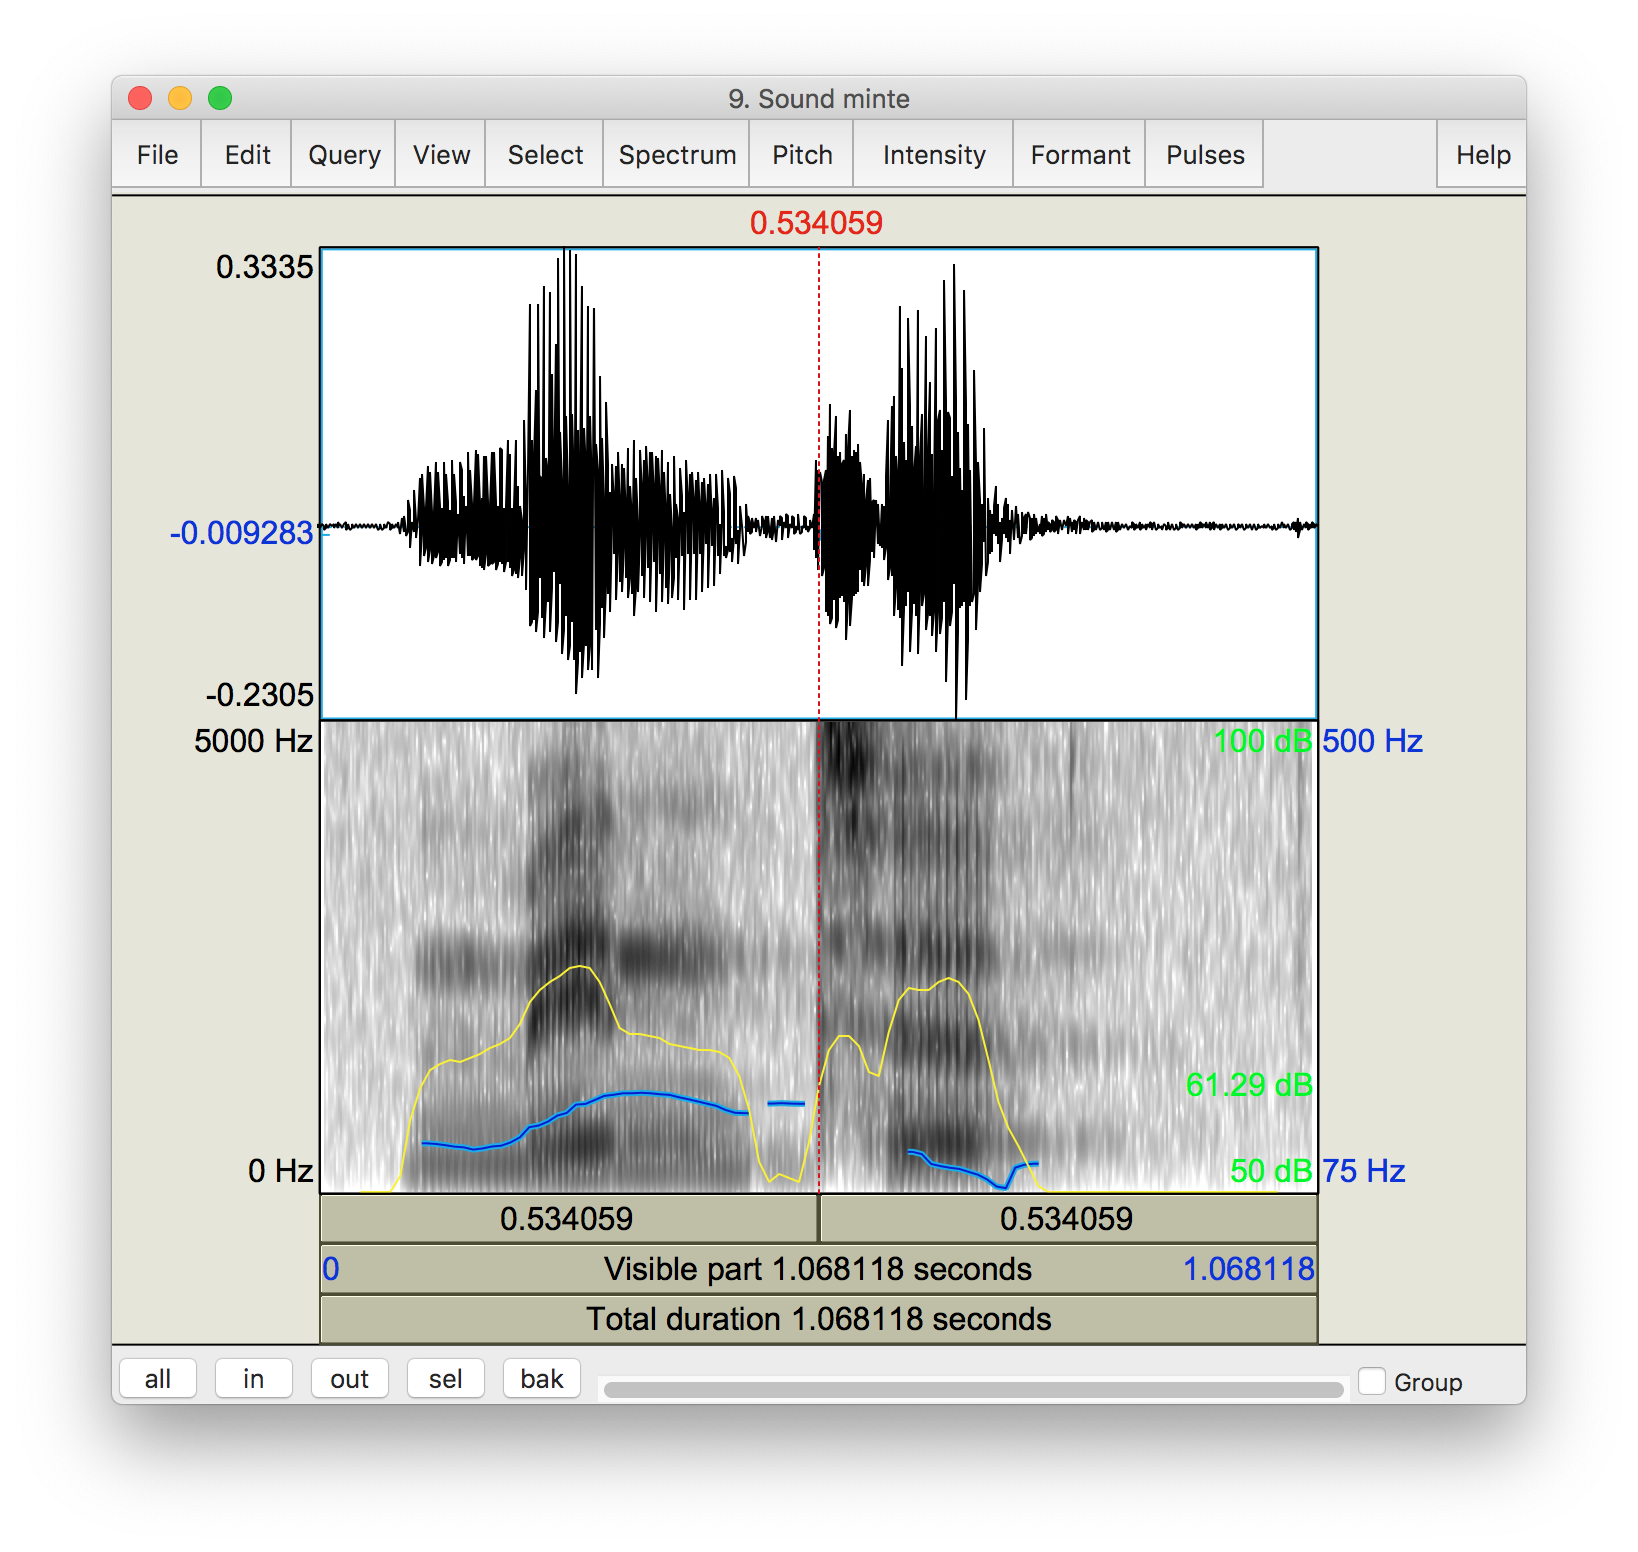
\includegraphics[height=0.8\textheight]{\GRAPHPATH/minte}
\end{frame}

\begin{frame}
  {Drucksilben und Schallsilben (Sievers, siehe \citealt{Maas2002})}
  \Large
  \textit{Miete}\\
  \Zeile
  \centering
  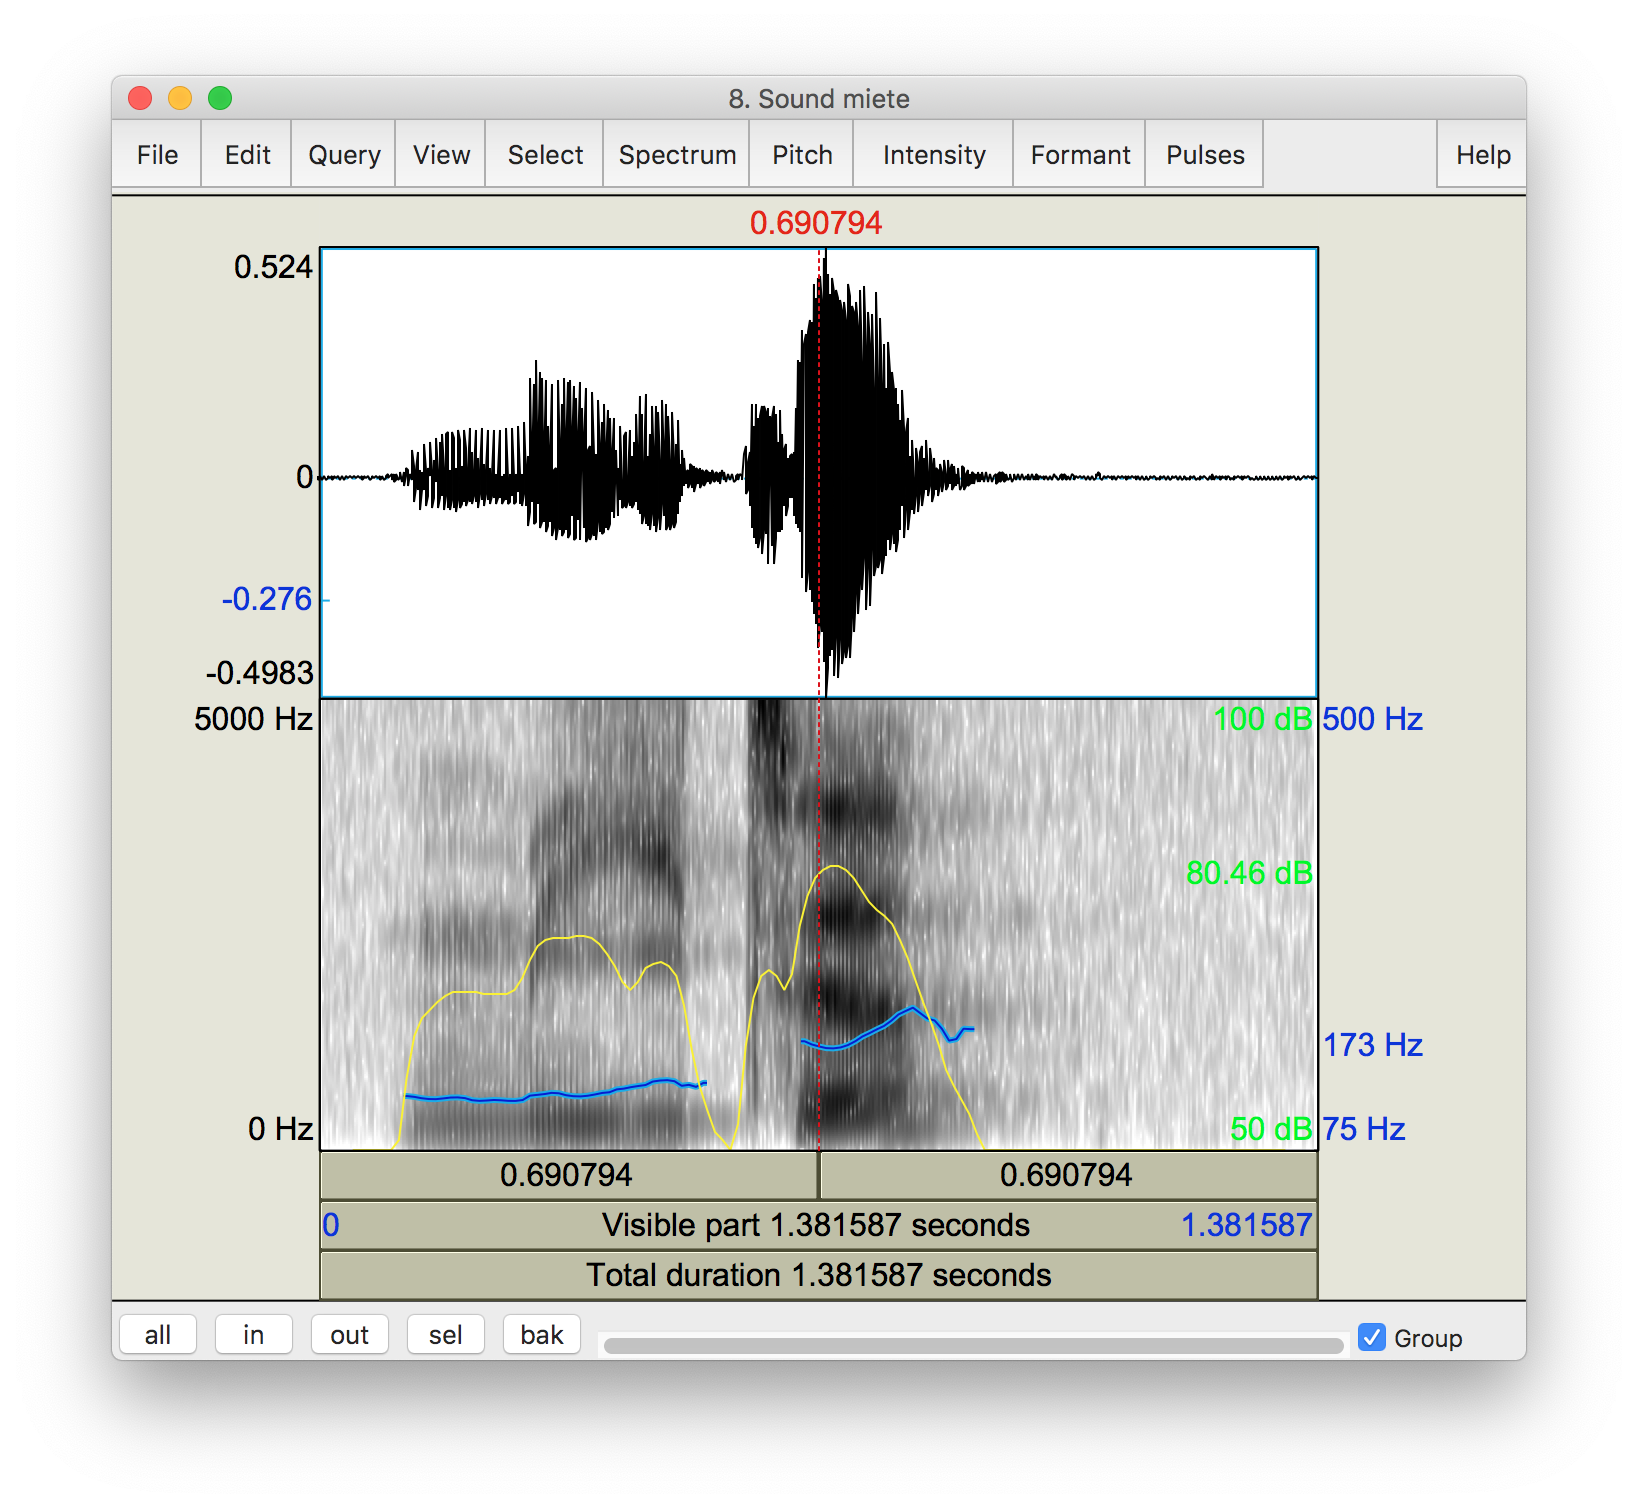
\includegraphics[height=0.8\textheight]{\GRAPHPATH/miete}
\end{frame}

\begin{frame}
  {Drucksilben und Schallsilben (Sievers, siehe \citealt{Maas2002})}
  \Large
  \textit{Mitte}\\
  \Zeile
  \centering
  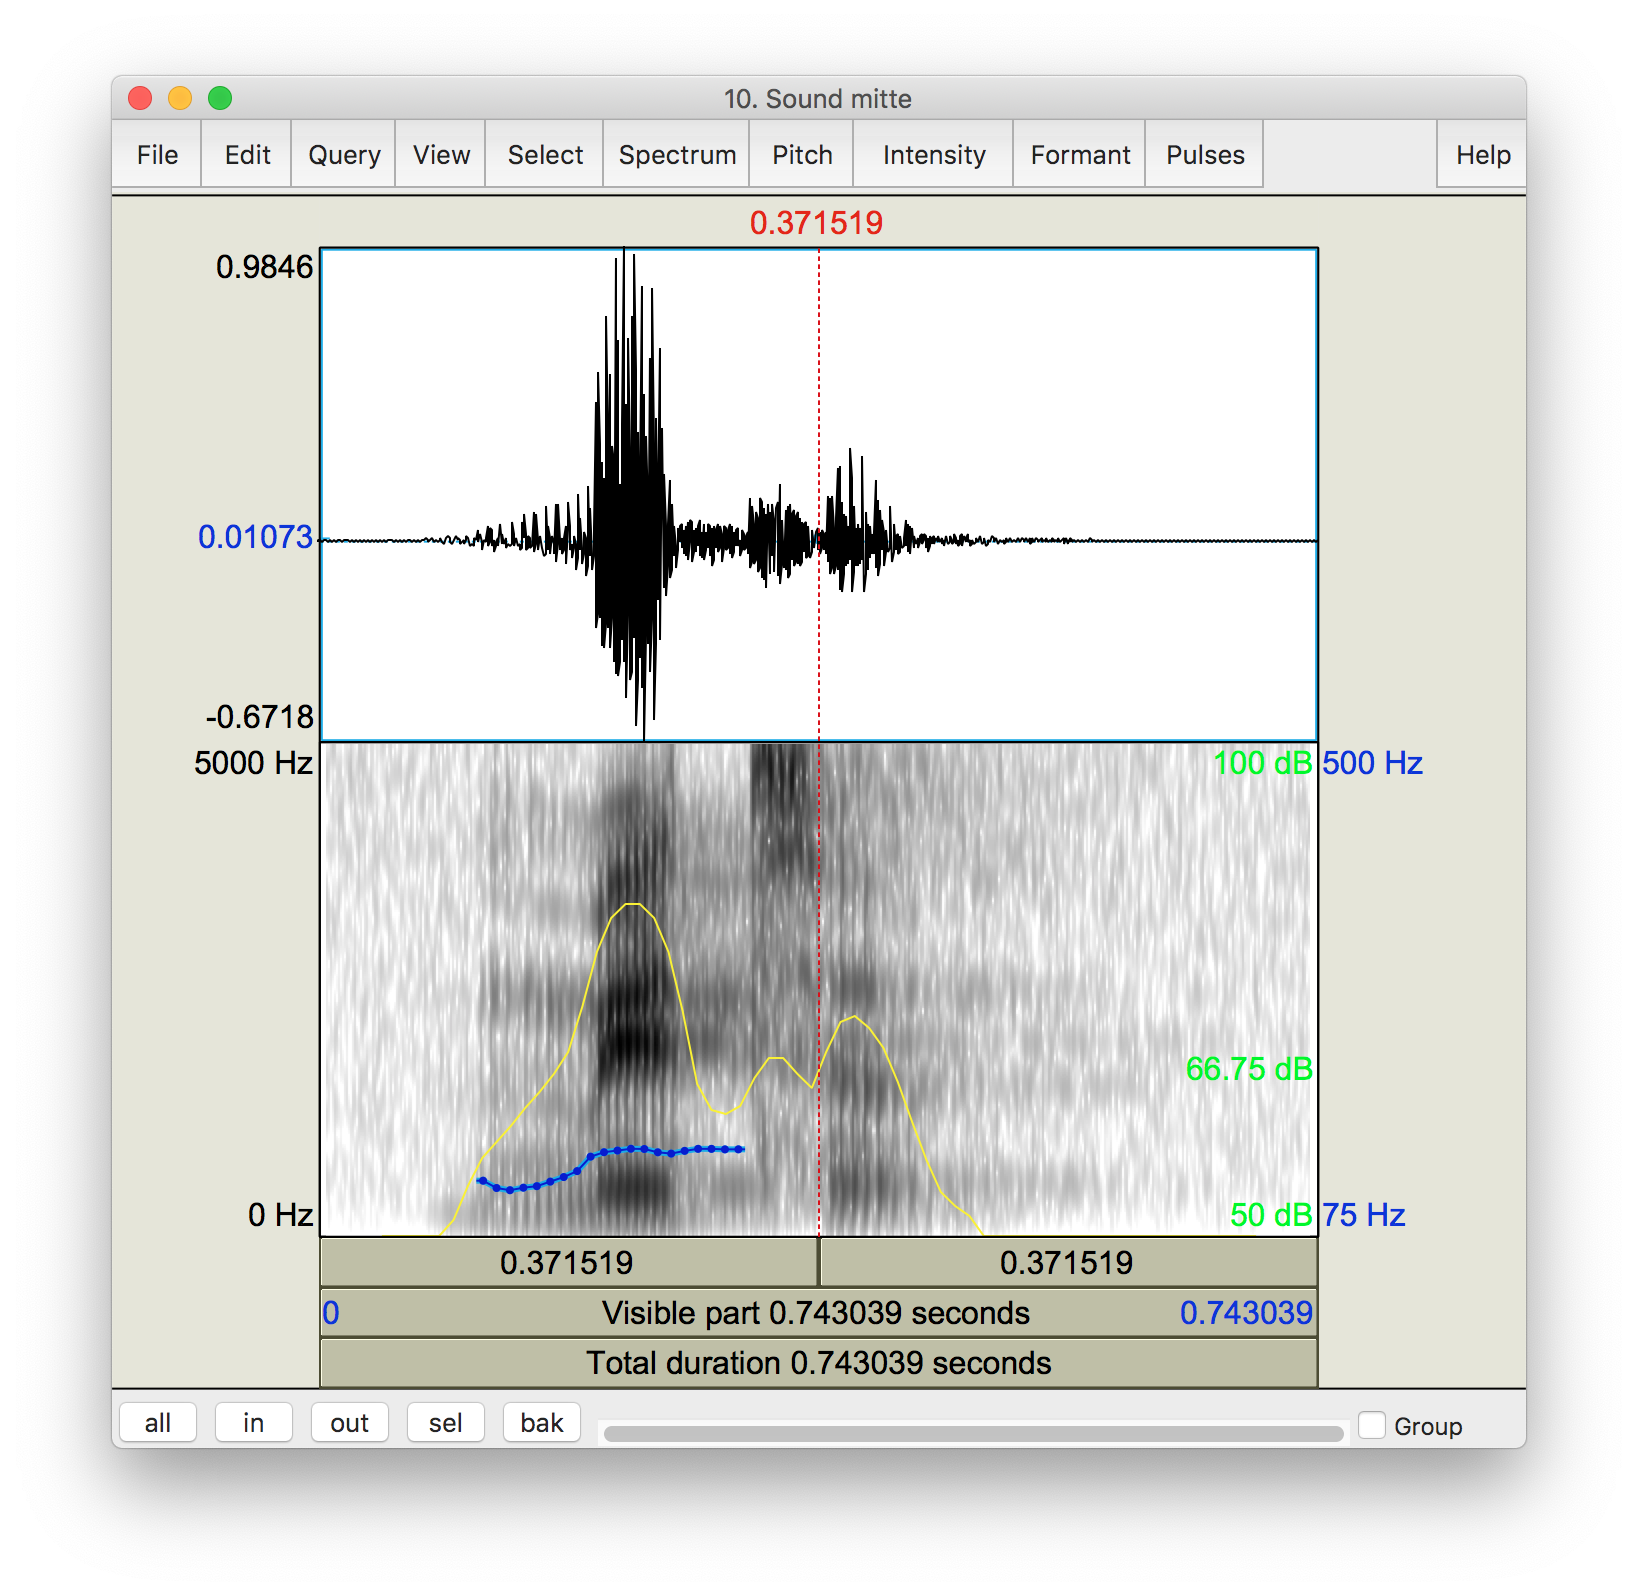
\includegraphics[height=0.8\textheight]{\GRAPHPATH/mitte}
\end{frame}

\begin{frame}
  {Nachtrag zu EGBD3}
  \pause
  In EGBD3 steht, einmorige Silben gäbe es nur mit Schwa\ldots
  \pause
  \Zeile
  \begin{itemize}[<+->]
    \item \textit{bläulichere} /blɔ͡ʏlɪçəʁə/ $\Rightarrow$ [ˈblɔ͡ʏ.l\rot{ɪ}.çə.ʁə]
    \item \textit{Neunziger} /nɔ͡ʏnt͡sɪgəʁ/ $\Rightarrow$ [ˈnɔ͡ʏn.t͡s\rot{ɪ}.gɐ]
    \item \textit{unterschiedliche} /ʊntəʁʃidlɪçə/ $\Rightarrow$ [ˈʔʊn.tɐ.ʃiːd.l\rot{ɪ}.çə]
  \end{itemize}
  \pause
  \Halbzeile
  \begin{alertblock}{Korrektur: einmorige Silben mit Nicht-Schwa}
    In abgeleiteten mehrsilbigen Wörtern können \rot{nur in unbetonten Silben}\\
    überleichte Silben mit anderen Vokalen als Schwa auftreten. Dabei wird \\
    \rot{kein Silbengelenk} gebildet. Es handelt sich im Wesentlichen um [ɪ] in\\
    abgeleiteten Adjektiven.
  \end{alertblock}
%   \pause
%   \Zeile
%   Achtung: Da \textit{-in} einen Nebenakzent trägt, liegt in \textit{Schülerinnen} /ʃyləʁɪnən/ $\Rightarrow$ [ˈʃyː.lə.ˌʁɪṇən] und ähnlichen Wörtern ein Silbengelenk vor!
\end{frame}


\begin{frame}
  {Maximierung des Anfangsrands}
  \pause
  Es bleiben immer noch Zweifelsfälle bei der wortinternen Silbifizierung\dots\\
  \pause
  \Zeile
  \begin{exe}
    \ex\textit{freches} \alert{[fʁɛç̣əs]}, \rot{*[fʁɛç.əs]}
    \pause
    \ex\textit{komplett} \alert{[kɔm.plɛt]}, \rot{*[kɔmp.lɛt]}
    \pause
    \ex\textit{Betreff} \alert{[bə.tʁɛf]}, \rot{*[bət.ʁɛf]}
  \end{exe}
  \Zeile
  \pause
  \Large
  Strukturbedingung: So viele Konsonanten wie möglich\\
  in den \alert{Anfangsrand} statt in den Endrand packen!\\
\end{frame}


\begin{frame}
  {Die Klatschmethode und die Hinhörschreibung}
  \pause
  "`Hinhörschreibungen"'?\\
  \begin{itemize}[<+->]
    \item E\rot{h}e, we\rot{h}e
    \item Ra\rot{d}, Wan\rot{d}, Bun\rot{d}
    \item bri\rot{ng}, Go\rot{ng}
    \item Köni\rot{g}, weni\rot{g}, wichti\rot{g}
    \item \rot{S}tein, \rot{S}palte
  \end{itemize}
  \pause
  "`Klatschmethode"'?\\
  \begin{itemize}[<+->]
    \item Krie\rot{ch}er, rö\rot{tl}ich, Nö\rot{rgl}er, a\rot{bsp}a\rot{lt}en, Ä\rot{rzt}e, plö\rot{tzl}ich
    \item rate, ratte
    \item Matsche
    \item Küche
    \item bringe
  \end{itemize}
\end{frame}


\begin{frame}
  {Und wie geht es richtig?}
  \pause
  \Large
  \Zeile\Zeile
  \begin{center}
    Denken Sie da mal drüber nach!
  \end{center}
%   \Halbzeile
%   Ganz allgemein wichtig für Grammatikvermittlung:\\
%  \Halbzeile 
%  \pause
%  \begin{itemize}[<+->]
%     \item Was ist die \alert{Fähigkeit}, die vermittelt werden soll?
%     \item Welches \alert{Wissen} ist nötig, um diese zu erwerben?
%     \item Welchen \alert{Übungs-Input} müssen Sie den Lernenden geben?
%   \end{itemize}
%  \Halbzeile
%  \pause
%   Mögliches Vorgehen:
%   \pause
%   \begin{itemize}[<+->]
%     \item \alert{Bewusstsein für Länge}
%     \item Bewusstsein für \alert{Länge je nach Position}
%     \item kurz vor Vokal im Wort $\Rightarrow$ Silbengelenk, Gelenkschreibung
%     \item \rot{Formenreihen als Ausgangsbasis}: \alert{nur Kernwortschatz}
%     \item Anfang mit dem \alert{Einsilbler} (ohne Dehnungsschreibung?)
%     \item weiter mit dem \alert{trochäischen Zweisilbler ohne Silbengelenk}
%     \item schließlich \alert{Zweisilbler mit Silbengelenk}
%   \end{itemize}
\end{frame}

\section{Vorschau}

\begin{frame}
  {Nächste Woche: Wortklassen und Wortarten}
  \pause
  \begin{itemize}[<+->]
    \item Was sind Wörter?
    \item Sind Wortklassen durch \alert{Bedeutungen} definiert?
    \item \alert{morphologische} Definitionen von Wortklassen
    \item \alert{syntaktische} Definitionen von Wortklassen
    \item \alert{Wie viele Wortklassen gibt es?}
  \end{itemize}
  \pause
  \Zeile
  \centering
  \Large
  \alert{Bitte lesen: Kapitel 6 komplett,\\
  mindestens aber 6.2 (S.~174--191)}
  \pause
  \pause
  \pause
  \pause
  \pause
\end{frame}


  
  \let\subsection\section\let\section\woopsi
  \section{Wortklassen}
  \let\woopsi\section\let\section\subsection\let\subsection\subsubsection
  
\section{Rückblick}

\begin{frame}
  {Silbenphonologie}
  \pause
  \begin{itemize}[<+->]
    \item Silben sind nicht lexikalisch\slash zugrundeliegend.
    \item Sonorität: Öffnen und Schließen des Vokaltrakts
    \item Sonoritätskontur: Anstieg zum Vokal, dann Abfall
    \item Anfangsrand, Kern, Endrand; Reim
    \item \alert{extrasilbische} Sonoritätsverletzungen: /ʃ/, /s/, /t/
    \item prototypischer komplexe Anfangsrand: \alert{Obstruent + Liquid}
    \item prototypischer komplexe Endrand: \alert{Liquid + Obstruent}
    \item Wichtig: \alert{Das gilt für betonte Silben im Kernwortschatz.}
    \item Silbengewicht in \alert{Moren} (Vokal: eine\slash zwei, Kons.: je eine)
    \item Überschwere: verhindert durch Extrasilbizität
    \item Silbengelenk: geteilter Konsonant statt überleichter Silbe im Trochäus
    \item Anfangsrandmaximierung bei Zweifelsfällen der Silbifizierung
  \end{itemize}
\end{frame}

\begin{frame}
  {Warum Reim?}
  \pause
  \begin{itemize}[<+->]
    \item Reim = Kern und Endrand
    \item \alert{Für das Silbengewicht zählt nur der Reim!}
    \item Prinzip: eigene Regularität → eigene Struktur
      \Zeile
    \item außerdem: literarischer \alert{Endreim}: \alert{Anfangsrand egal}
    \item und: literarischer \alert{Anfangsreim} (Stabreim): \alert{Silbenreim egal} 
  \end{itemize}
\end{frame}

\begin{frame}
  {Alfred Lichtenstein: Die Dämmerung}
  \pause
  \small
  Ein dicker Junge spielt mit einem \textbf{\rot<3>{T}\alert<3>{eich}}.\\
  Der Wind hat sich in einem Baum ge\textbf{\rot<4>{f}\alert<4>{an}}/gen.\\
  Der Himmel sieht verbummelt aus und \textbf{\rot<3>{bl}\alert<3>{eich}},\\
  Als wäre ihm die Schminke ausge\textbf{\rot<4>{g}\alert<4>{an}}/gen.\\
  \Zeile
  Auf lange Krücken schief herabge\textbf{\rot<5>{b}\alert<5>{ückt}}\\
  Und schwatzend kriechen auf dem Feld zwei \textbf{\rot<6>{L}\alert<6>{ah}}|me.\\
  Ein blonder Dichter wird vielleicht ver\textbf{\rot<5>{r}\alert<5>{ückt}}.\\
  Ein Pferdchen stolpert über eine \textbf{\rot<6>{D}\alert<6>{a}}|me.\\
  \Zeile
  An einem Fenster klebt ein fetter \textbf{\rot<7>{M}\alert<7>{ann}}.\\
  Ein Jüngling will ein weiches Weib be\textbf{\rot<8>{s}\alert<8>{u}}|chen.\\
  Ein grauer Clown zieht sich die Stiefel \textbf{\alert<7>{an}}.\\
  Ein Kinderwagen schreit und Hunde \textbf{\rot<8>{fl}\alert<8>{u}}|chen.\\
  \Zeile
  \footnotesize
  Aus: Pinthus, Kurt (Hrsg.). 1920. \textit{Menschheitsdämmerung}. Berlin: Rowohlt. S.~11.\\
  Mit | sind normale Silbengrenzen und mit / Silbengelenke markiert.
\end{frame}


\section{Überblick}

\begin{frame}
  {Überblick}
  \pause
  \begin{itemize}[<+->]
    \item Was sind Wörter?
    \item Lexikalisches vs.\ syntaktisches Wort
      \Zeile
    \item Wozu Wortklassen?
    \item \rot{Bedeutungsklassen} und Wortklassen
    \item \alert{Morphologie} von Wortklassen
    \item \alert{Syntax} von Wortklassen
      \Zeile
    \item wichtige Wortklassen
      \begin{itemize}[<+->]
        \item Nomen
        \item Verb
        \item Präposition
        \item Komplementierer
        \item Adverb
        \item Partikel
      \end{itemize}
  \end{itemize}
\end{frame}

\begin{frame}
  {Wortklassen und Bildungssprache\slash Lehramt}
  \pause
  \begin{itemize}[<+->]
    \item direkter Einfluss von Wortklassenwissen auf\\
      bildungssprachliche Fähigkeiten: \rot{keiner}
      \Zeile
    \item Sprachbetrachtung (Woche 1):
      \begin{itemize}[<+->]
        \item \rot{Form} → \alert{Funktion}
        \item \rot{systematisch}, also basierend auf \alert{Generalisierungen}
        \item essentiell für formale Generalisierungen: \alert{Wortklassen}
      \end{itemize}
      \Zeile
    \item Normfragen und Wortklassenbezug
      \begin{itemize}
        \item \alert{Substantivgroßschreibung}
        \item Nebensätze: Komplementierer, Pronomina, Kommas
        \item Flexion (Problemfälle: Konjunktiv, Adjektive usw.)
        \item \dots alles nicht ohne Wortklassen beschreibbar
      \end{itemize}
  \end{itemize}
\end{frame}

\section{Wörter}

\begin{frame}
  {Ebenen und Einheiten}
  \pause
  \begin{itemize}[<+->]
    \item Wortakzent: \textit{\alert{\textbf{Sie}}ges\alert{säu}le}\\
      $\rightarrow$ phonologisches\slash prosodisches Wort
      \Zeile
    \item Eigenschaften von Wörtern jenseits der Phonologie?
  \end{itemize}
  \Zeile
  \pause
  \begin{exe}
    \ex
    \begin{xlist}
      \ex[]{Staat-es}
      \pause
      \ex[*]{Tür-es}
    \end{xlist}
    \pause
    \Zeile
    \ex
    \begin{xlist}
      \ex[]{Der Satz ist eine grammatische Einheit.}
      \pause
      \ex[*]{Die Satz ist eine grammatische Einheit.}
    \end{xlist}
  \end{exe}
\end{frame}

\begin{frame}
  {Wört haben eine Bedeutung?}
  \pause
  \begin{exe}
    \ex \alert{Es} \alert{wird} schon wieder früh dunkel.
    \pause
    \ex Kristine denkt, \alert{dass} \alert{es} bald regnen \alert{wird}.
    \pause
    \ex Adrianna \alert{hat} gestern \alert{den} Keller inspiziert.
    \pause
    \ex Camilla \alert{und} Emma sehen \alert{sich} \alert{die} Fotos \alert{an}.
  \end{exe}
  \Zeile
  \pause
  \large
  \alert{Bedeutungstragende Wörter und Funktionswörter}
\end{frame}

\begin{frame}
  {Morphologie und Syntax}
  \pause
  \begin{itemize}[<+->]
    \item Kombinatorik für \alert{Wortbestandteile}: Morphologie
      \begin{itemize}[<+->]
        \item Wortbestandteile \zB mit \alert{Umlaut}: \textit{rot} -- \textit{röter}
        \item oder \alert{Ablaut}: \textit{heben} -- \textit{hob}
      \end{itemize}
    \item Kombinatorik für \alert{Wörter}: Syntax
      \Zeile
    \item \alert{Zirkuläre oder leere Definitionen?}
    \item \rot{Nein!} Prinzip: eigene Regularität → eigene Struktur
      \Zeile
    \item Wortbestandteile \alert{nicht trennbar}:
      \begin{itemize}
        \item \textit{heb-t}\\
          *\textit{heb mit Mühe t}
        \item \textit{Ge-hob-en-heit} \\
          *\textit{Gehoben anspruchsvolle heit}
        \item \textit{Sie geht schnell heim.}\\
          \textit{Schnell geht sie heim.}
      \end{itemize}
  \end{itemize}
\end{frame}

\begin{frame}
  {Wort und Wortform I}
  \pause
  \begin{exe}
    \ex
    \begin{xlist}
      \ex (der) Tisch
      \pause
      \ex (den) Tisch
      \pause
      \ex (dem) Tisch\alert{e}
      \pause
      \ex (des) Tisch\alert{es}
      \pause
      \ex (die) Tisch\alert{e}
      \pause
      \ex (den) Tisch\alert{en}
    \end{xlist}
  \end{exe}
  \pause
  \begin{exe}
    \ex
    \begin{xlist}
      \ex Der \_\_\_\ ist voll hässlich.
      \pause
      \ex Ich kaufe den \_\_\_ nicht.
      \pause
      \ex Wir speisten am \_\_\_\ des Bundespräsidenten.
      \pause
      \ex Der Preis des \_\_\_\ ist eine Unverschämtheit.
      \pause
      \ex Die \_\_\_\ kosten nur noch die Hälfte.
      \pause
      \ex Mit den \_\_\_\ können wir nichts mehr anfangen.
    \end{xlist}
  \end{exe}
\end{frame}

\begin{frame}
  {Wort und Wortform II}
  \pause
  \begin{block}{Wortform}
    Eine Wortform ist eine in syntaktischen Strukturen auftretende und in diesen Strukturen nicht weiter zu unterteilende Einheit.
    Die Werte der Merkmale von Wortformen sind gemäß ihrem Paradigma vollständig spezifiziert.
  \end{block}
  \Zeile
  \pause
  \begin{block}{Lexikalisches Wort}
    Das (\alert{lexikalische}) \alert{Wort} ist eine Repräsentation von paradigmatisch zusammengehörenden Wortformen.
    Für das lexikalische Wort sind die Werte nur für diejenigen Merkmale spezifiziert, die in allen Wortformen des Paradigmas dieselben Werte haben.
    Die restlichen Werte werden gemäß der Position im Paradigma bei den konkret vorkommenden Wortformen des Wortes gesetzt.
  \end{block}
\end{frame}

\section{Methode}

\begin{frame}
  {Klassische Grundschul-Wortarten}
  \pause
  \scalebox{0.85}{%
  \begin{minipage}{\textwidth}
    \begin{itemize}[<+->]
      \item Dingwort
      \item Tuwort, Tätigkeitswort
      \item Wiewort, Eigenschaftswort
      \item Umstandswort
      \item Noch besser die Vermittlungsversuche:
        \begin{itemize}[<+->]
          \item Dingwörter kann man anfassen. \onslide<8->{\rot{D'oh!}}
            \pause
          \item Wie ist die Kanzlerin? -- Katatonisch.
          \item Was macht Johanna? -- Laufen.
          \item Wie, wo oder warum schläft Johanna? -- Ruhig.
        \end{itemize}
      \item Wieso auch nicht?
        \begin{itemize}[<+->]
          \item Anfassen? Wolken, Ideen, Steckdosen, Rasierklingen, \dots
          \item *Die Kanzlerin ist ehemalig.
          \item Was macht Johanna? -- Hausaufgaben.
          \item Was tut Johanna? -- *Verlaufen. \slash *Unterliegen.
          \item *Was macht\slash tut das Yoghurt? -- Verschimmeln.
          \item Wie schläft Johanna? -- *Erstaunlicherweise.
        \end{itemize}
    \end{itemize}
  \end{minipage}
  }
\end{frame}

\begin{frame}
  {Ein paar neue Wortarten nach Bedeutungen I}
  \pause
  \begin{itemize}[<+->]
    \item "`Wie, wo, warum?"' \onslide<3->{--- Warum eigentlich nicht drei Wortarten?}
      \Halbzeile
      \pause
    \item \alert{Bewegungsverben}: \textit{laufen}, \textit{springen}, \textit{fahren}, \dots
    \item \alert{Zustandsverben}: \textit{duften}, \textit{wohnen}, \textit{liegen}, \dots
      \Halbzeile
    \item \alert{Konkreta}: \textit{Haus}, \textit{Buch}, \textit{Blume}, \textit{Stier}, \dots
    \item \alert{Abstrakta}: \textit{Konzept}, \textit{Glaube}, \textit{Wunder}, \textit{Kausalität}, \dots
    \item \alert{Zählsubstantive}: \textit{Kumquat}, \textit{Student*in}, \textit{Mikrobe}, \textit{Kneipe}, \dots
    \item \alert{Stoffsubstantive}: \textit{Wasser}, \textit{Wein}, \textit{Zement}, \textit{Mehl}, \dots
  \end{itemize}
\end{frame}

\begin{frame}
  {Ein paar neue Wortarten nach Bedeutungen II}
  \pause
  Aber Moment mal\dots\\
  \pause
  \Zeile
  \begin{exe}
    \ex
    \begin{xlist}
      \ex \alert{Wein} kann lecker sein.
      \ex \alert{Kumquats können}\slash \alert{Eine Kumquat kann} lecker sein.
    \end{xlist}
%     \pause
%     \ex
%     \begin{xlist}
%       \ex Ein Glas \alert{guter Wein}\slash\alert{guten Weins} kostet 10€.
%       \ex Ein Glas \alert{?gute Kumquats}\slash\alert{guter Kumquats} kostet 4€.
%     \end{xlist}
%     \pause
%     \ex
%     \begin{xlist}
%       \ex Johanna hätte gerne \alert{eine Kumquat}.
%       \ex Johanna hätter gerne \alert{einen Wein}.
%     \end{xlist}
  \end{exe}
  \pause
  \Zeile
  Es gibt hier durchaus auch \alert{formale} Unterschiede.
\end{frame}

\begin{frame}
  {Morphologische Klassifikation}
  \pause
  \begin{exe}
    \ex
    \begin{xlist}
      \ex{Ich pfeif\alert{e}.\\
      Du pfeif\alert{st}.\\
      Die Schiedsrichterin pfeif\alert{t}.}
        \pause
        \ex{Ich schlaf\alert{e}.\\
        {Du schl\rot{ä}f\alert{st}.}\\
        Die Schiedsrichterin schl\rot{ä}f\alert{t}.}
    \end{xlist}
        \pause
    \ex
    \begin{xlist}
      \ex{der Berg\\
        des Berg\alert{es}\\
        die Berg\alert{e}}
        \pause
      \ex{der Mensch\\
        des Mensch\alert{en}\\
        die Mensch\alert{en}}
        \pause
      \ex{der Staat\\
        des Staat\alert{es}\\
        die Staat\alert{en}}
    \end{xlist}
  \end{exe}
\end{frame}

\begin{frame}
  {Achtung!}
  \pause
  \alert{Änderung der Paradigmenzugehörigkeit} eines Wortes:
  \pause
  \Zeile
  \begin{exe}
    \ex\label{ex:paradigmatischeklassifikation017}\begin{xlist}
      \ex{Wir sind des \alert{Wanderns} müde.}
      \pause
      \ex{Wir \alert{wandern}.}
    \end{xlist}
  \end{exe}
  \pause
  \Zeile
  $\Rightarrow$ \rot{Zwei verschiedene} lexikalische Wörter.
\end{frame}


\begin{frame}
  {Syntaktische Klassifikation}
  \pause
  \begin{exe}
    \ex
    \begin{xlist}
      \ex[]{Alexandra spielt schnell \alert{und} präzise.}
      \pause
      \ex[*]{Alexandra spielt schnell \alert{obwohl} präzise.}
      \pause
      \ex[]{Alexandra \alert{und} Dzsenifer spielen eine gute Saison.}
      \pause
      \ex[*]{Alexandra \alert{obwohl} Dzsenifer spielen eine gute Saison.}
    \end{xlist}
    \pause
    \Zeile
    \ex
    \begin{xlist}
      \ex[]{Alexandra spielt herausragend,\\
        \alert{obwohl} der Leistungsdruck hoch ist.}
      \pause
      \ex[*]{Alexandra spielt herausragend, \alert{und} der Leistungsdruck hoch ist.}
    \end{xlist}
  \end{exe}
    \pause
    \Zeile
    Alles nur wegen der Bedeutung?
    \pause
  \begin{exe}
    \ex Der Marmorkuchen spielt schnell \alert{und} präzise.
  \end{exe}
\end{frame}

\begin{frame}[fragile]
  {Filter}
  \begin{itemize}
    \item<2-> Kapitel 2: \alert{Kategorien} definiert über Merkmale und Werte.
      \begin{itemize}[<+->]
        \item<3-> Hat \textsc{Numerus} oder nicht?
        \item<4-> Hat \textsc{Genus} oder nicht?
        \item<5-> \dots
      \end{itemize}
  \end{itemize}
  \begin{center}
    \scalebox{0.7}{
    \begin{minipage}{\textwidth}  
    \begin{forest}
      /tikz/every node/.append style={font=\footnotesize},
      for tree={l sep=2em, s sep=2.5em},
      [\textit{Wort}, intrme, {visible on=<6->}, for children={visible on=<7->}
        [{Hat  Numerus?}, decide, for children={visible on=<8->}
          [\textit{flektierbar}, intrme, yes, {visible on=<9->}, for children={visible on=<11->}
            [{Ist finit  flektierbar?}, decide, {visible on=<11->}, for children={visible on=<12->}
              [\textbf{Verb}, finall, yes, {visible on=<13->}]
              [\textit{Nomen}, intrme, no, {visible on=<14->}]
            ]
          ]
          [\textit{nicht flektierbar}, intrme, no, {visible on=<10->}, for children={visible on=<15->}
            [{Hat Valenz-\slash  Kasusrektion?}, decide, {visible on=<15->}, for children={visible on=<16->}
              [\textbf{Präposition}, finall, yes, {visible on=<17->}]
              [\textit{andere}, intrme, no, {visible on=<18->}]
            ]
          ]
        ]
      ]
    \end{forest}
   \end{minipage}
   }
  \end{center}
\end{frame}


\section{Wortklassen}

\begin{frame}
  {Flektierbare Wörter: Numerus}
  \pause
  \begin{exe}
    \ex
    \begin{xlist}
      \ex Tüte, Tüten
      \pause
      \ex Baum, Bäume
    \end{xlist}
    \pause
    \ex
    \begin{xlist}
      \ex (ich) gehe, (wir) gehen
      \pause
      \ex (du) gehst, (ihr) geht
    \end{xlist}
    \Zeile
    \pause
    \ex
    \begin{xlist}
      \ex \alert<12->{Ein} \alert<13->{roter} \alert<8->{Apfel} \alert<9->{hängt} am Baum.
      \pause
      \ex \alert<14->{Rote} \alert<10->{Äpfel} \alert<11->{hängen} am Baum.
    \end{xlist}
  \end{exe}
  \Zeile
  \pause
  \pause
  \pause
  \pause
  \pause
  \pause
  \pause
  \pause
  Als \alert{Kongruenzmerkmal} ist Numerus in der Definition\\
  der flektierbaren Wortklassen \alert{strukturell motiviert}.
\end{frame}

\begin{frame}
  {Substantive vs.\ Nomina}
  \pause
  \begin{exe}
    \ex \alert<5->{Die stärkste} Gewichtheberin wurde Weltmeisterin.
    \pause
    \ex \alert<5->{Der stärkste} Versuch war der zweite.
    \pause
    \ex \alert<5->{Das höchste} Gewicht wurde von Tatjana gerissen.
  \end{exe}
  \Zeile
  \pause
  \pause
  \begin{itemize}[<+->]
    \item Substantive: festes Genus
    \item andere Nomina (Artikel\slash Pronomen, Adjektiv):\\
      \alert{Genuskongruenz mit dem Substantiv}
  \end{itemize}
\end{frame}

\begin{frame}
  {Adjektive}
  \pause
  \begin{exe}
    \ex
    \begin{xlist}
      \ex Kein \alert<3->{großer} Ball wurde gespielt.
      \ex Der \alert<3->{große} Ball wurde gespielt.
    \end{xlist}
    \pause
    \pause
    \ex
    \begin{xlist}
      \ex Keine \alert<5->{großen} Bälle wurden gespielt.
      \ex Die \alert<5->{großen} Bälle wurden gespielt.
      \ex Große \alert<5->{Bälle} wurden gespielt.
    \end{xlist}
  \end{exe}
  \Zeile
  \pause
  \pause
  \centering
  \resizebox{0.4\textwidth}{!}{
    \begin{tabular}{lllllll}
      \toprule
      \multicolumn{3}{l}{} & \textbf{Mask} & \textbf{Neut} & \textbf{Fem} & \textbf{Pl} \\
      \midrule
      \multirow{4}{*}{\textbf{stark}} & \textbf{Nom} & \multirow{4}{*}{heiß-} & er & es & e & e \\
      & \textbf{Akk} && en & es & e & e \\
      & \textbf{Dat} && em & em & er & en \\
      & \textbf{Gen} && en & en & er & er \\
      \midrule
      \multirow{4}{*}{\textbf{schwach}} & \textbf{Nom} & \multirow{4}{*}{(der) heiß-} & e & e & e & en \\
      & \textbf{Akk} && en & e & e & en \\
      & \textbf{Dat} && en & en & en & en \\
      & \textbf{Gen} && en & en & en & en \\
      \midrule
      \multirow{4}{*}{\textbf{gemischt}} & \textbf{Nom} & \multirow{4}{*}{(kein) heiß-} & er \Dim & es \Dim & e & en \\
      & \textbf{Akk} && en & es \Dim & e & en \\
      & \textbf{Dat} && en & en & en & en \\
      & \textbf{Gen} && en & en & en & en \\
      \bottomrule
    \end{tabular}
  }
\end{frame}

\begin{frame}
  {Präpositionen}
  \pause
  \begin{exe}
    \ex
    \begin{xlist}
      \ex{\alert<3-4>{Mit} \alert<4>{dem kaputten Rasen} ist nichts mehr anzufangen.}
      \pause
      \pause
      \pause
      \ex{\alert<6-7>{Angesichts} \alert<7>{des kaputten Rasens} wurde das Spiel abgesagt.}
    \end{xlist}
  \end{exe}
  \pause
  \pause
  \pause
  \Zeile
  \begin{block}{Rektion}
    In einer Rektionsrelation werden durch die regierende Einheit (das \alert{Regens}) Werte für bestimmte Merkmale (und ggf.\ auch die Form) beim regierten Element (dem \alert{Rectum}) verlangt.\\
  \end{block}
  \Zeile
  \pause
  \begin{block}{Präposition}
    Präpositionen kasusregieren eine obligatorische Nominalphrase.
  \end{block}
\end{frame}

\begin{frame}
  {Komplementierer}
  \pause
  \begin{exe}
    \ex
    \begin{xlist}
      \ex[]{Ich glaube, [\alert<3->{dass} dieser Nebensatz ein Verb \alert<4->{enthält}].}
      \ex[]{[\alert<6->{Während} die Spielzeit \alert<7->{läuft}], zählt jedes Tor.}
      \ex[]{Es fällt ihnen schwer [\rot<8->{zu laufen}].}
      \ex[\rot<11->{*}]{[\alert<9->{Obwohl} kein Tor \alert<10->{fiel}].}
    \end{xlist}
  \end{exe}
  \Zeile
  \pause
  \pause
  \pause
  \pause
  \pause
  \pause
  \pause
  \pause
  \pause
  \pause
  \begin{block}{Komplementierer}
    Komplementierer leiten Nebensätze ein.\\
    Die Rede von der \textit{unterordnenden Konjunktion} ist ungeschickt.
  \end{block}
\end{frame}

\begin{frame}
  {Nicht-flektierbare Wörter im Vorfeld}
  \pause
  Was steht im unabhängigen Aussagesatz am Satzanfang?\\
  \pause
  {\rot{Antworten Sie nie mehr mit "`das Subjekt"'!}}
  \pause
  \begin{exe}
    \ex\label{ex:adverbenadkopulasundpartikeln038}
    \begin{xlist}
      \ex[ ]{\alert<5->{Gestern} hat der FCR Duisburg gewonnen.}
      \pause
      \pause
      \ex[ ]{\alert<7->{Erfreulicherweise} hat der FCR Duisburg gestern gewonnen.}
      \pause
      \pause
      \ex[ ]{\alert<9->{Oben} finden wir andere Beispiele.}
      \pause
      \pause
      \ex[*]{\alert<11->{Doch} ist das aber nicht das Ende der Saison.}
      \pause
      \pause
      \ex[*]{\alert<13->{Und} ist die Saison zuende.}
      \pause
      \pause
    \end{xlist}
    \ex\label{ex:adverbenadkopulasundpartikeln044} Das ist aber \alert{doch} nicht das Ende der Saison.
  \end{exe}
  \pause
  \Viertelzeile
  \begin{block}{Adverb}
    Adverben sind die übriggebliebenen nicht-flektierbaren Wörter, die im Vorfeld stehen können.
  \end{block}
\end{frame}

\begin{frame}
  {Adkopulas}
  \pause
  Kopulas: \textit{sein}, \textit{bleiben}, \textit{werden}\\
  \pause
  Spezielle Klasse von Hilfsverben\dots
  \pause
  \Zeile
  \begin{exe}
    \ex
    \begin{xlist}
      \ex[ ]{Hamlet \alert<6->{ist} \alert<5->{meschugge}.}
      \pause
      \pause
      \pause
      \ex[ ]{\alert<8->{Quitt} \alert<9->{bin} ich mit dir noch lange nicht.}
      \pause
      \pause
      \pause
    \end{xlist}
    \Zeile
    \ex
    \begin{xlist}
      \ex[ ]{Tatjana \alert<11->{ist} \alert<12->{stark}.}
      \pause
      \pause
      \pause
      \ex[ ]{Die \alert<14->{starke} \alert<15->{Gewichtheberin} ist Weltmeisterin.}
      \pause
      \pause
      \pause
    \end{xlist}
    \Zeile
    \ex
    \begin{xlist}
      \ex[ ]{Der Staat \alert<18->{ist} \alert<17->{pleite}.}
      \pause
      \pause
      \pause
      \ex[*]{Der \alert<20->{pleite} \alert<21->{Staat} bricht zusammen.}
      \pause
      \pause
      \pause
    \end{xlist}
  \end{exe}
  \begin{block}{Adkopula}
    Adkopulas treten immer in Abhängigkeit einer Kopula auf.
  \end{block}
\end{frame}

\begin{frame}
  {Konjunktionen}
  \pause
  \begin{exe}
    \ex\label{ex:konjunktionen052}
    \begin{xlist}
      \ex{[Dzsenifer] \alert<3->{und} [eine andere Spielerin] haben Tore geschossen.}
      \pause
      \pause
      \ex{Sätze können wir [aufschreiben] \alert<5->{oder} [aussprechen].}
      \pause
      \pause
      \ex{Spielt bitte [konzentriert] \alert<7->{und} [offensiv].}
      \pause
      \pause
    \end{xlist}
  \end{exe}
  \Zeile
  \begin{block}{Konjunktion}
    Konjunktionen verbinden Satzteile der gleichen Kategorie.\\
    Die Rede von der \textit{neben-}\slash\textit{beiordnenden Konjunktion} ist ungeschickt. 
  \end{block}
\end{frame}

\begin{frame}[fragile]
  {"`Alle Wortklassen"'}
  \pause
  \begin{center}
    \scalebox{0.35}{
    \begin{minipage}{\textwidth}
    \centering
    \begin{forest}
      /tikz/every node/.append style={font=\footnotesize},
      for tree={l sep=2em, s sep=2.5em, align=center},
      [\textit{Wort}, intrme
        [{Hat\\Numerus?}, decide
          [\textit{flektierbar}, intrme, yes
            [{Ist finit\\flektierbar?}, decide
              [\textbf{Verb}, finall, yes]
              [\textit{Nomen}, intrme, no
                [{Hat festes\\Genus?}, decide
                  [\textbf{Substantiv}, finall, yes]
                  [{\textit{anderes}\\\textit{Nomen}}, intrme, no
                    [{Hat Stärke-\\flexion?}, decide
                      [\textbf{Adjektiv}, finall, yes]
                      [{\textit{Artikel\slash}\\\textit{Pronomen}}, intrme, no]
                    ]
                  ]
                ]
              ]
            ]
          ]
          [\textit{nicht flektierbar}, intrme, no
          [{Hat Valenz-\slash\\Kasusrektion?}, decide
              [\textbf{Präposition}, finall, yes]
              [\textit{andere}, intrme, no
                [{Leitet Neben-\\Sätze ein?}, decide
                  [\textbf{Komplementierer}, finall, yes]
                  [{\textit{Partikel\slash}\\\textit{Adverb}}, intrme, no
                    [{Kann das Vor-\\feld besetzen?}, decide
                      [{\textit{Adverb\slash}\\\textit{Adkopula}}, intrme, yes
                        [{Wird typisch mit\\Kopula verwendet?}, decide
                          [\textbf{Adkopula}, finall, yes]
                          [\textbf{Adverb}, finall, no]
                        ]
                      ]
                      [\textit{Partikel}, intrme, no
                        [{Kann Sätze\\ersetzen?}, decide
                          [\textbf{Satzäquivalent}, finall, yes]
                          [\textit{andere}, intrme, no
                            [{Kann Konsti-\\tuenten verbinden?}, decide
                              [\textbf{Konjunktion}, finall, yes]
                              [\textit{Rest}, intrme, no]
                            ]
                          ]
                        ]
                      ]
                    ]
                  ]
                ]
              ]
            ]
          ]
        ]
      ]
    \end{forest}
    \end{minipage}
    }
  \end{center}
\end{frame}

\begin{frame}
  {Wie viele Wortklassen gibt es?}
  \pause
  \begin{itemize}[<+->]
    \item Alle Wörter sind \alert{Wörter}.
    \item Also gibt es \rot{eine Wortklasse}.
      \Zeile
    \item Jedes Wort hat \alert{individuelle Eigenschaften}.
    \item Also gibt es \rot{so viele Wortklassen wie Wörter}.
      \Zeile
    \item Wozu brauchen wie überhaupt Wortklassen?\\
      Wortklassen\dots
      \begin{itemize}[<+->]
        \item \dots sind \alert{das Rüstzeug für Morphologie und Syntax}.
        \item \dots erlauben die Formulierung von \rot{Generalisierungen}.
        \item \dots sind so fein unterteilt, wie es unsere Beschreibung erfordert.
        \item \dots sind \rot{nicht universell}!
        \item \dots sind \alert{Artefakte unserer Theorie bzw.\ Grammatik}.
      \end{itemize}
  \end{itemize}
\end{frame}

\section{Vorschau}

\begin{frame}
  {Morphologie}
  \pause
  \textit{"`Das ist wegen der Spannendheit."'}\\
  \pause
  \textit{"`Die Vase ist vollansichtlich reliefiert."}\\
  \Zeile
  \pause
  \begin{itemize}[<+->]
    \item (Wort-)Formen, ihre Bestandteile und ihre Funktionen
    \item Umlaut und Ablaut und ihre Funktionen
    \item Unterschied von Flexion und Wortbildung
      \Zeile
    \item Funktion nominaler Flexionskategorien
    \item \rot{Wichtig!} \alert{Inklusive: Was ist Kasus?}
    \item Funktionen verbaler Flexionskategorien
    \item \rot{Wichtig!} \alert{Inklusive: Was ist Tempus?}
  \end{itemize}
  \pause
  \Zeile
  \centering
  Bitte lesen: \alert{Kapitel 7 (195--220), 9.1 (248--257), 10.1 (287--299)}

  \pause
  \pause
  \pause
  \pause
  \pause
\end{frame}


  
  \let\subsection\section\let\section\woopsi
  \section{Morphologie}
  \let\woopsi\section\let\section\subsection\let\subsection\subsubsection
  
\section{Rückblick}

\begin{frame}
  {Wortklassen: Grundlagen}
  \pause
  \begin{itemize}[<+->]
    \item Wortklassen als \alert{Grundausstattung der Grammatik}
    \item Vehikel für klassenbezogene Generalisierungen
    \item Bedeutung? --- nicht alle Wörter
      \Zeile
    \item Wortform\slash syntaktisches Wort:
      \begin{itemize}[<+->]
        \item konkrete Form \alert{im syntaktischen Kontext}
        \item voll spezifiziert (Merkmale, Werte)
      \end{itemize}
      \Zeile
    \item Wort\slash lexikalisches Wort:
      \begin{itemize}[<+->]
        \item abstrakte Form \alert{im Lexikon}
        \item evtl.\ unterspezifiziert
      \end{itemize}
      \Zeile
    \item "`Schulwortarten"': \alert{unzureichend operationalisiert}
  \end{itemize}
\end{frame}

\section{Überblick}

\begin{frame}
  {Morphologie: Flexion und Wortbildung}
  \pause
  \begin{itemize}[<+->]
    \item \alert{Formveränderungen} und \alert{Merkmalsänderungen}
      \begin{itemize}[<+->]
        \item Veränderungen von Werten
        \item Veränderungen von Merkmalsaustattungen
      \end{itemize}
      \Halbzeile
    \item Morphe (= Wortbestandteile) und ihre Funktionen
    \item Morphe: alle Stämme und alle nicht-lexikalischen Morphe
    \item Umlaut und Ablaut (bzw.\ Vokalstufen)
      \Halbzeile
    \item statische und volatile Merkmale
    \item Wortbildung vs.\ Flexion, definiert anhand von Merkmalen
  \end{itemize}
\end{frame}

\begin{frame}
  {Morphologie und Bildungssprache\slash Normsprache}
  \pause
  \begin{itemize}[<+->]
    \item Flexion und zugehörige Funktionskategorien
      \begin{itemize}[<+->]
        \item normsprachlich überwiegend \alert{klar definiert}
        \item vorliterate perfekte Beherrschung nicht voraussetzbar (z.\,B.\ Konjunktiv)
          \Halbzeile
        \item erhebliche Abweichungen in \alert{Dialekten}, \alert{Soziolekten} und \alert{Kiezsprachen}
          \Halbzeile
        \item \textit{Et rēchnet aufe Terasse.} (Pott)
        \item Aber wie funktioniert das eigentlich genau?
          \Halbzeile
        \item \textit{Ich las schon einmal Rilke.} (rhfr. Hyperkorrektur)
        \item Im Odenwald gibt es kein Präteritum, wird in der Schule gelernt.
      \end{itemize}
     \Halbzeile 
    \item Wortbildung
      \begin{itemize}[<+->]
        \item wichtiger Kern der Bildungssprache (besonders Komposition)
          \Halbzeile
        \item \textit{Das ist wegen der Spannendheit.} (Kind, 7--8 Jahre, ca. 1992)
        \item \textit{Die Vase ist vollansichtlich reliefiert.} (Heide Rezepa-Zabel, 2018)
      \end{itemize}
  \end{itemize}
\end{frame}

\begin{frame}
  {Morphosyntax in der Schule}
  \pause
  Wozu ist so ein Unterricht gut?
  \pause
  \begin{center}
    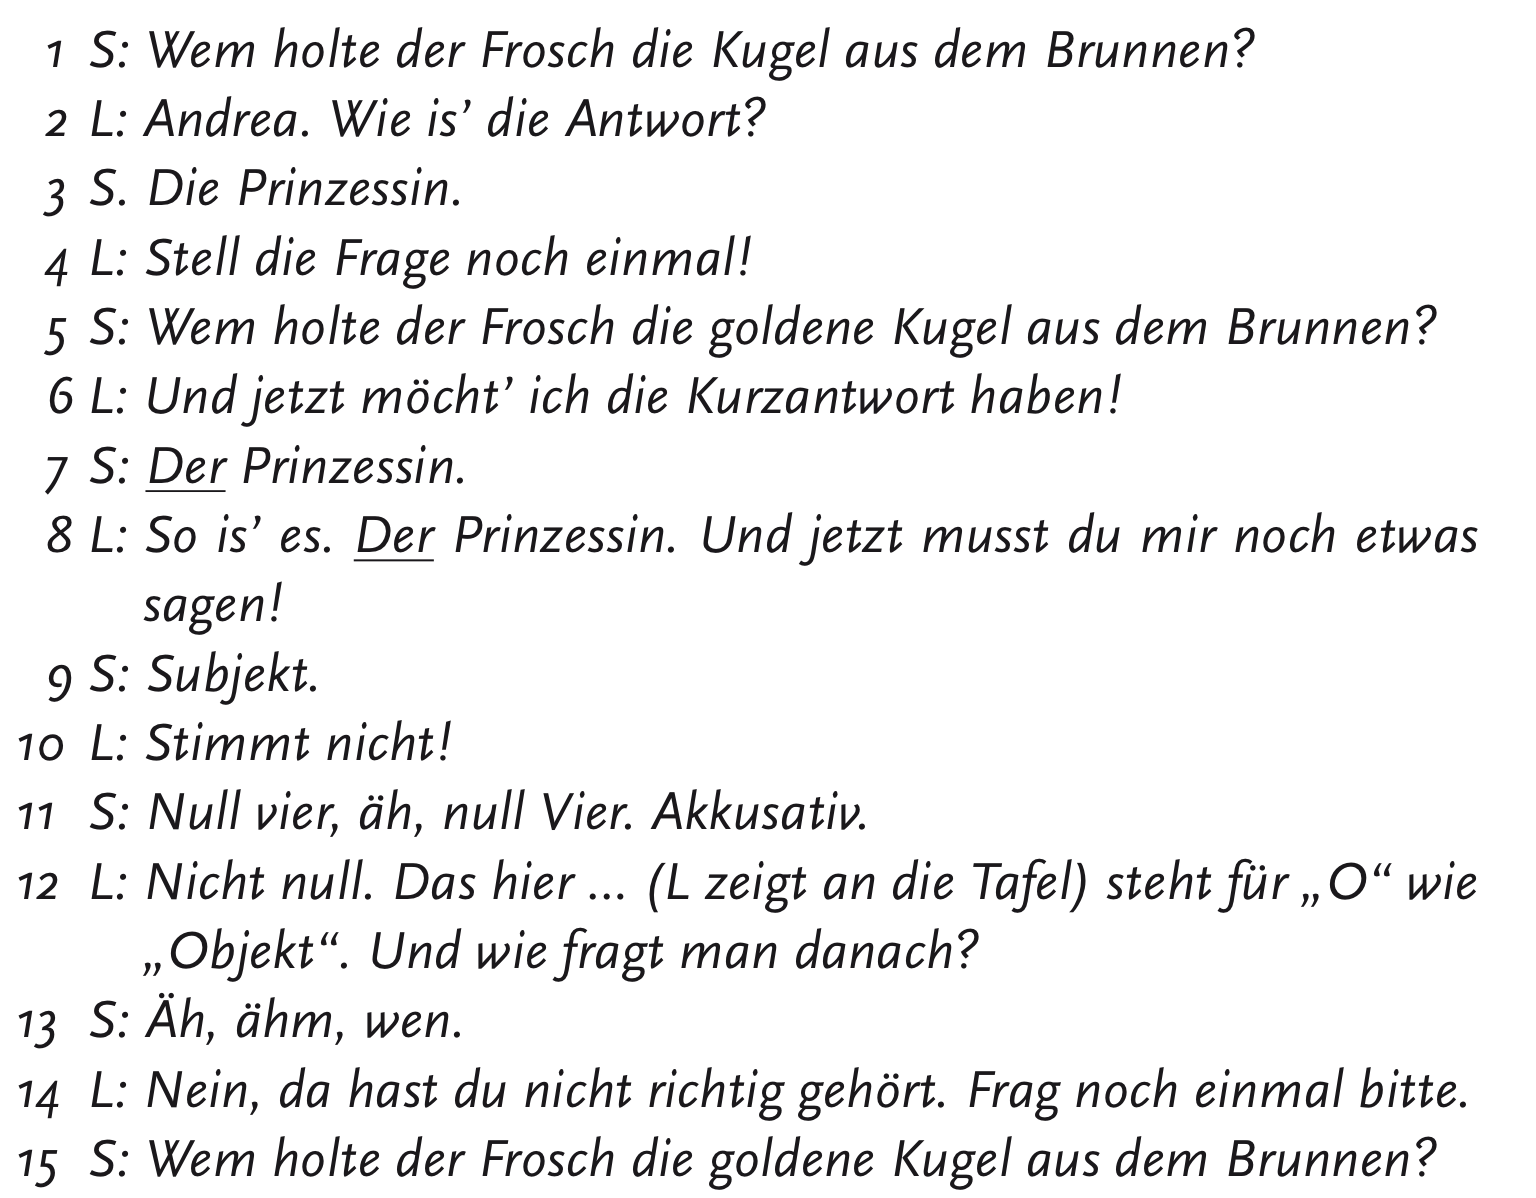
\includegraphics[width=0.6\textwidth]{graphics/kasusschule1}
  \end{center}
  \tiny \citet[36--37]{Gramzowemden2002}, zitiert nach \citet[257--258]{Bredel2013}
\end{frame}

\begin{frame}
  {Morphosyntax in der Schule}
  Wozu ist so ein Unterricht gut?
  \begin{center}
    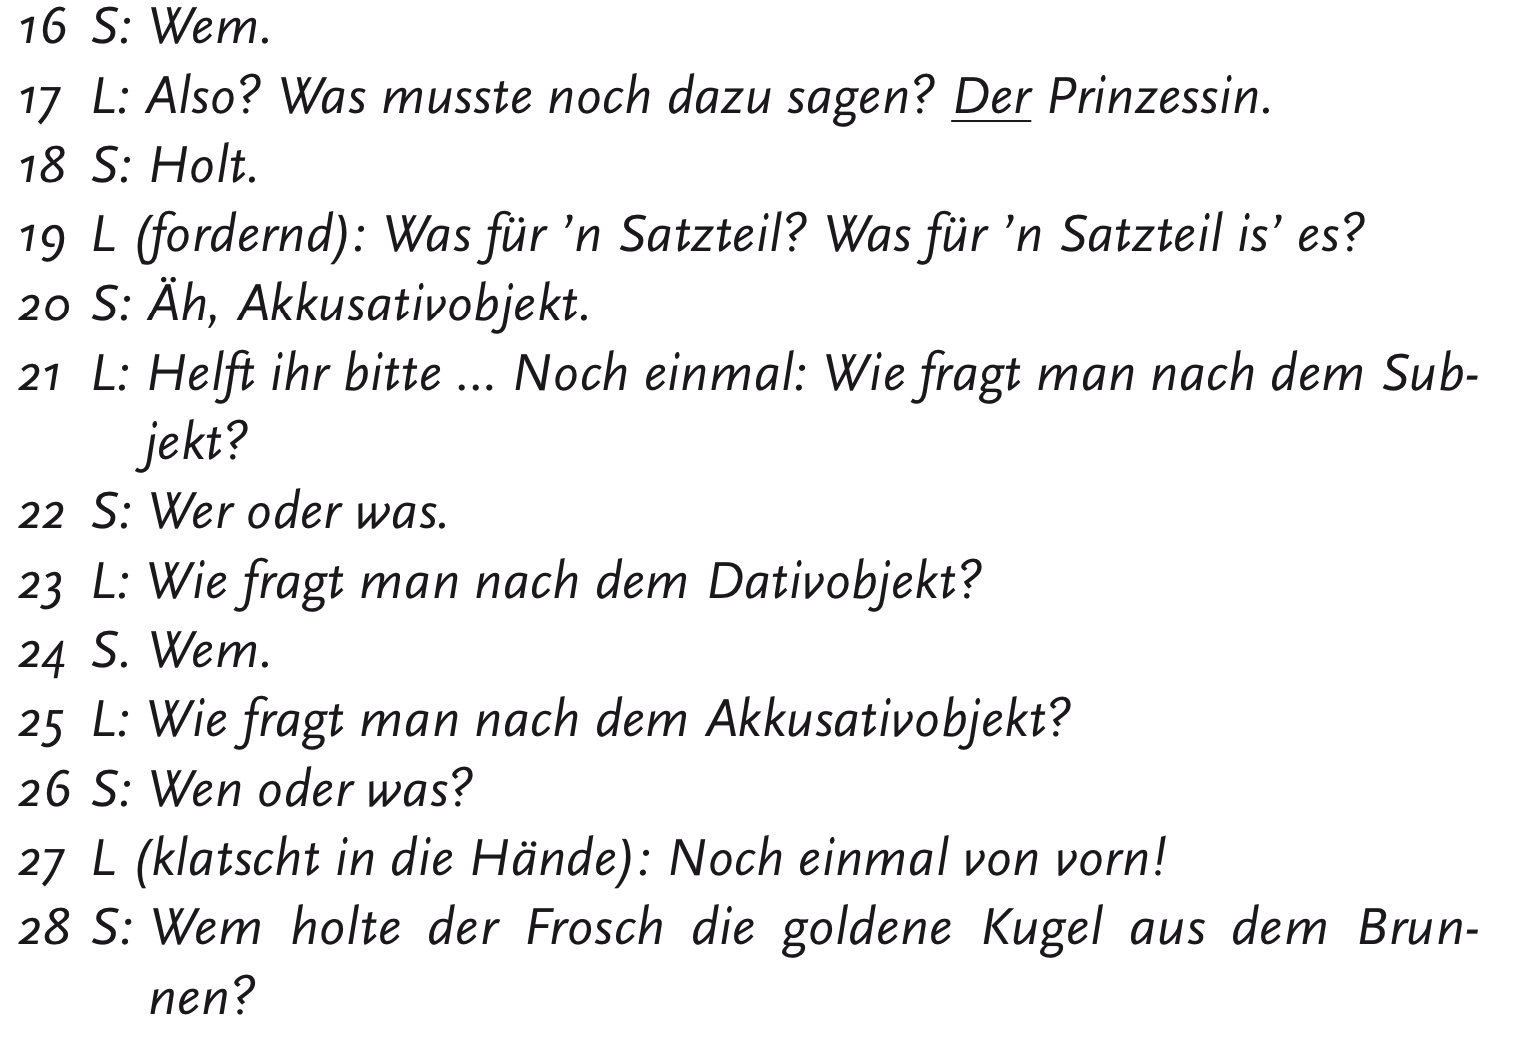
\includegraphics[width=0.6\textwidth]{graphics/kasusschule2}
  \end{center}
  \tiny \citet[36--37]{Gramzowemden2002}, zitiert nach \citet[257--258]{Bredel2013}
\end{frame}

\begin{frame}
  {Morphosyntax in der Schule}
  Wozu ist so ein Unterricht gut?
  \begin{center}
    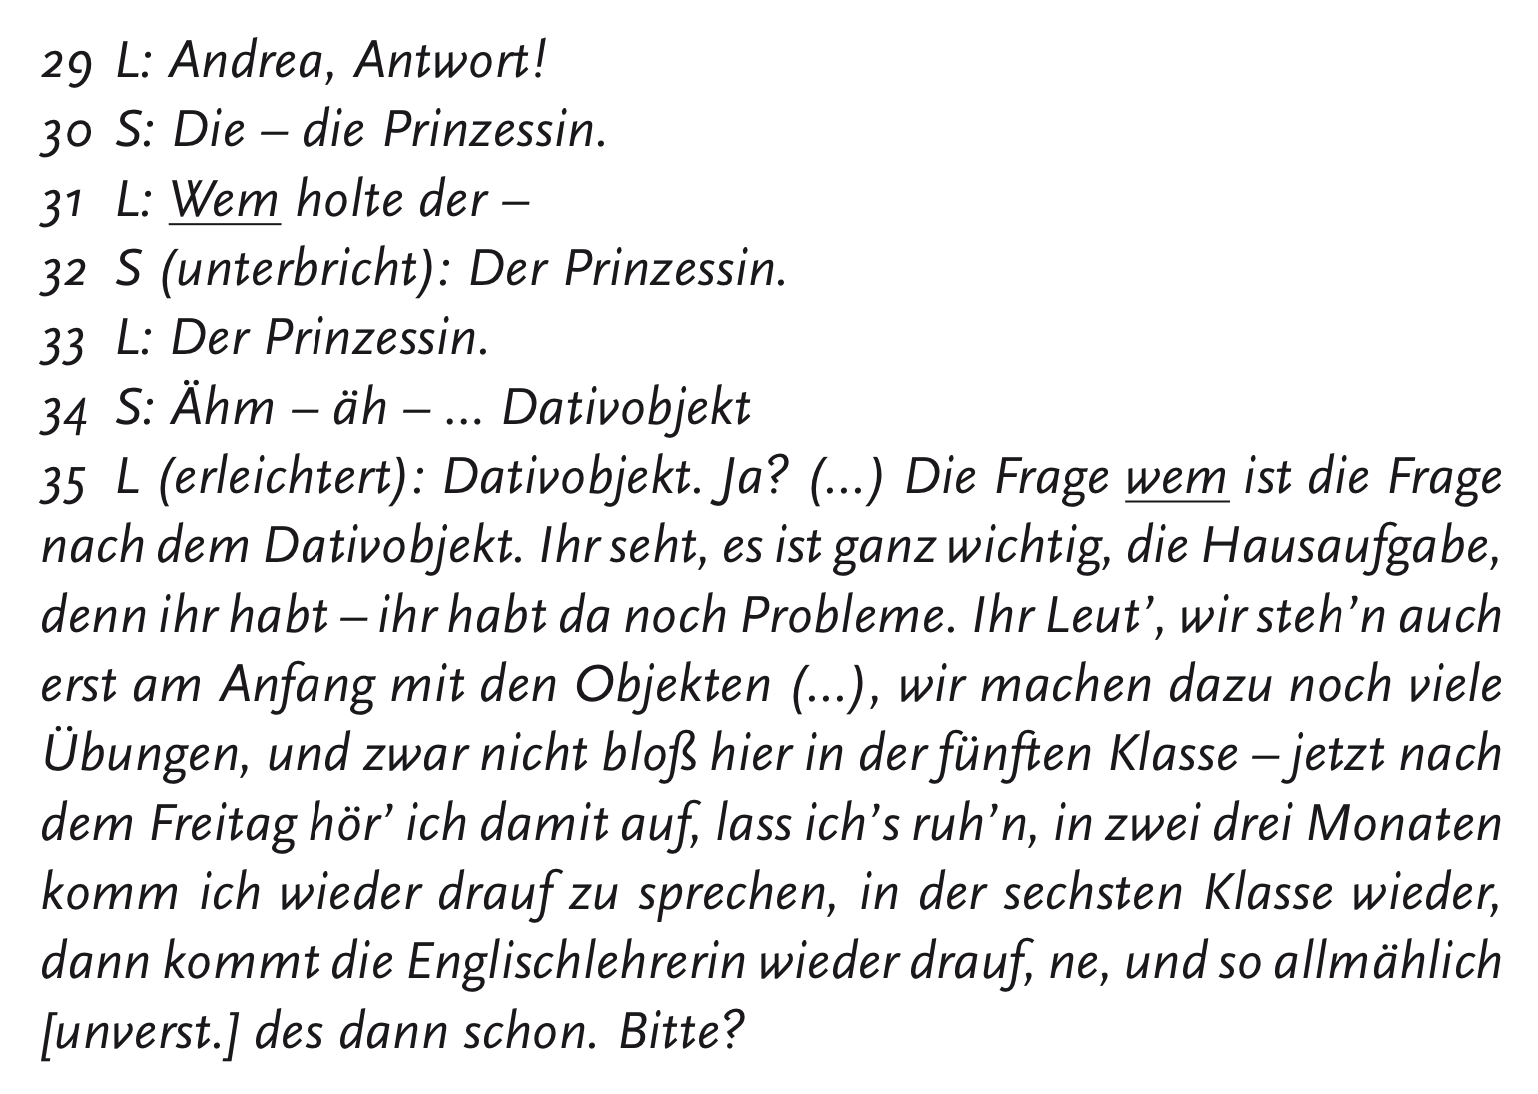
\includegraphics[width=0.6\textwidth]{graphics/kasusschule3}
  \end{center}
  \tiny \citet[36--37]{Gramzowemden2002}, zitiert nach \citet[257--258]{Bredel2013}
\end{frame}

\section{Stämme und Affixe}

\begin{frame}
  {Form und Funktion: Flexion}
  \pause
  \begin{exe}
    \ex
    \begin{xlist}
      \ex \alert{Den Präsidenten} begrüßte \alert{der Dekan} äußerst respektlos.
      \pause
      \ex \alert{Der Dekan} begrüßte \alert{den Präsidenten} äußerst respektlos.
    \end{xlist}
    \pause
    \ex
    \begin{xlist}
      \ex \alert{Die Präsidentin} begrüßte \alert{die Dekanin} äußerst respektlos.
      \pause
      \ex \alert{Die Dekanin} begrüßte \alert{die Präsidentin} äußerst respektlos.
    \end{xlist}
  \end{exe}
  \pause
  \Zeile
  Formveränderungen lexikalischer Wörter \alert{schränken ihre möglichen grammatischen Funktionen und Relationen im Satz ein}\dots\\
  \pause
  \Halbzeile
  \dots und sie haben semantische und systemexterne Folgen.

\end{frame}

\begin{frame}
  {Form und Funktion: Wortbildung}
  \pause
  \begin{exe}
    \ex grün\alert{lich}, röt\alert{lich}, gelb\alert{lich}
    \pause
    \ex Neu\alert{igkeit}, Blöd\alert{heit}, Tauch\alert{er}, Heb\alert{ung}
    \pause
    \ex Fenster\alert{rahmen}, Tücher\alert{spender}, Glas\alert{korken}, Unter\alert{schrank}
  \end{exe}
  \pause
  \Zeile
  Formveränderungen von einem zu einem anderen lexikalischen Wort führen zu Bedeutungs- und kategorialen Veränderungen.
\end{frame}

\begin{frame}
  {Markierungsfunktionen von Morphen I}
  \pause
  \begin{exe}
    \ex
    \begin{xlist}
      \ex{(der) \alert<4>{Berg}}
      \ex{(den) \alert<4>{Berg}}
      \ex{(dem) \alert<4>{Berg}}
      \ex{(des) \alert<5>{Berg}\rot<5>{-es}}
      \ex{(die) \alert<6>{Berg}\rot<6>{-e}}
      \ex{(der) \alert<6>{Berg}\rot<6>{-e}}
    \end{xlist}
    \pause
    \ex
    \begin{xlist}
      \ex{(der) \alert<8>{Mensch}}
      \ex{(den) \alert<9>{Mensch}\rot<9>{-en}}
      \ex{(dem) \alert<9>{Mensch}\rot<9>{-en}}
      \ex{(des) \alert<9>{Mensch}\rot<9>{-en}}
      \ex{(die) \alert<9>{Mensch}\rot<9>{-en}}
      \ex{(der) \alert<9>{Mensch}\rot<9>{-en}}
    \end{xlist}
  \end{exe}
\end{frame}

\begin{frame}
  {Markierungsfunktionen von Morphen II}
  \pause
  \begin{exe}
    \ex
    \begin{xlist}
      \ex{(ich) \alert<3>{kauf}\rot<3>{-e}}
      \ex{(du) \alert<4>{kauf}\rot<4>{-st}}
      \ex{(wir) \alert<5>{kauf}\rot<5>{-en}}
      \ex{(sie) \alert<5>{kauf}\rot<5>{-en}}
    \end{xlist}
  \end{exe}
\end{frame}

\begin{frame}
  {Morphe und Markierungsfunktionen}
  \pause
  \begin{itemize}[<+->]
    \item Formveränderungen:
      \begin{itemize}[<+->]
        \item oft nicht \alert{eine} Funktion
        \item \rot{Einschränkung} der möglichen Funktionen
      \end{itemize}
   \Halbzeile 
    \item \alert{Markierungsfunktion}: eine \alert{Reduktion}\\
      der möglichen Merkmale oder Werte einer Wortform
    \item zum Beispiel \textit{-en} bei schw.\ Maskulina: \rot{nicht} Nominativ Singular
    \item oder \textit{-en} bei Verben im Präsens: Plural und nicht adressatbezogen
      \Halbzeile
    \item \alert{Morphe = alle segmentalen Einheiten mit Markierungsfunktion}
    \item konkret: \alert{Stämme} und \alert{Affixe}
  \end{itemize}
\end{frame}

\begin{frame}
  {Stämme I}
  \pause
  \begin{exe}
    \ex
    \begin{xlist}
      \ex{(ich) \alert<5->{kauf}-e\\
        (du) \alert<5->{kauf}-st\\
        (ihr) \alert<5->{kauf}-t }
        \pause
        \ex{(ich) \alert<6->{kauf}-te\\
        (du) \alert<6->{kauf}-test\\
        (ihr) \alert<6->{kauf}-tet}
        \pause
        \ex{(ich habe) ge-\alert<7->{kauf}-t\\
        (du hast) ge-\alert<7->{kauf}-t\\
        (ihr habt) ge-\alert<7->{kauf}-t}
    \end{xlist}
  \end{exe}
\end{frame}

\begin{frame}
  {Stämme II}
  \begin{exe}
    \ex
    \begin{xlist}
      \ex{(ich) \alert<4->{nehm}-e\\
        (du) \rot<5->{nimm}-st\\
          (es) \rot<5->{nimm}-t\\
          (ihr) \alert<4->{nehm}-t}
        \pause
        \ex{(ich) \orongsch<6->{nahm}\\
        (du) \orongsch<6->{nahm}-st\\
          (ihr) \orongsch<6->{nahm}-t}
        \pause
        \ex{(ich habe) ge-\gruen<7->{nomm}-en\\
        (du hast) ge-\gruen<7->{nomm}-en\\
        (ihr habt) ge-\gruen<7->{nomm}-en}
    \end{xlist}
  \end{exe}
  \pause
  \pause
  \pause
  \pause
  \pause
  Der \alert{Stamm} kann nicht "`der unveränderliche Wortbestandteil"'\\
  eines lexikalischen Wortes (in einem Paradigma) sein.\\
  \Zeile
  \pause
  \alert{\dots aber der mit der Bedeutung, also der lexikalischen Markierungsfunktion}!
\end{frame}

\begin{frame}
  {Affixe}
  \pause
  \begin{exe}
    \ex
    \begin{xlist}
      \ex (ich) nehm\alert<6->{-e}
      \pause
      \ex (des) Berg\alert<7->{-es}
      \pause
      \ex Schön\alert<8->{-heit}
      \pause
      \ex \alert<9->{Un-}ding
    \end{xlist}
  \end{exe}
  \Zeile
  \pause
  \pause
  \pause
  \pause
  \pause
  \begin{itemize}[<+->]
    \item \alert{keine lexikalische Markierungsfunktion} (= keine eigene Bedeutung)
    \item \alert{nicht wortfähig} = nicht ohne Stamm verwendbar
  \end{itemize}
\end{frame}

\section{Umlaut und Ablaut}

\begin{frame}
  {Umlaut vs.\ Ablaut: Warum erst jetzt?}
  \pause
  \alert{"`So ein chaotisches Buch! Plötzlich geht es\\
  in der Morphologie wieder um Phonologie!"'}\pause --- Ja\dots
  \pause
  \Zeile
  \begin{itemize}[<+->]
    \item Morphophonologie
    \item Morphosyntax
    \item Syntax-Semantik-Schnittstelle
    \item Prosodie-Pragmatik-Schnittstelle
    \item usw.
      \Zeile
    \item \rot{Die Grammatik nutzt die verfügbaren Mittel gut aus,\\
      und Markierungsmöglichkeiten aller Ebenen können\\
    auf anderen Ebenen zum Einsatz kommen.}
  \end{itemize}
\end{frame}

\begin{frame}[fragile]
  {Umlaut}
  \pause
  \begin{center}
    \resizebox{0.4\textwidth}{!}{
    \begin{tikzpicture}[scale=3.5,baseline=default]
      \large
      \tikzset{
        vowel/.style={fill=white, anchor=mid, text depth=0ex, text height=1ex},
        vowelgespannt/.style={circle,fill=gray!30, anchor=mid, text depth=0ex, text height=1ex,minimum size=4ex},
        dot/.style={circle,fill=black,minimum size=0.4ex,inner sep=0pt,outer sep=-1pt},
      }

      \coordinate (hf) at (0,2); % high front
      \coordinate (hb) at (2,2); % high back
      \coordinate (lf) at (1,0); % low front
      \coordinate (lb) at (2,0); % low back
      \def\V(#1,#2){barycentric cs:hf={(3-#1)*(2-#2)},hb={(3-#1)*#2},lf={#1*(2-#2)},lb={#1*#2}}

      % Chart key (vorne -- hinten).
      \draw [{Latex[round]}-] (\V (-.25,0)) -- (\V (-.25,.5)) node[above left] {\footnotesize vorne};
      \draw [-{Latex[round]}] (\V (-.25,1.5)) -- (\V (-.25,2)) node[above left] {\footnotesize hinten};
      \path (\V (-.25,1)) node[above] {\footnotesize zentral};

      % Chart key (hoch -- tief).
      \draw [{Latex[round]}-] (\V (0,-.25)) -- +(270:.5cm) node[above right,rotate=90] (vokaltrapez1) {\footnotesize hoch};
      \draw [{Latex[round]}-] (\V (3,-2.5)) -- +(270:-.5cm) node[above left,rotate=90] (vokaltrapez2) {\footnotesize tief};
      \path (\V (1.5,-1)) node[above,rotate=90] {\footnotesize mittel};

      % Grid.
      \draw [gray, thick] (\V(0,0)) -- (\V(0,2));
      \draw [gray, thick] (\V(3,0)) -- (\V(3,2));
      \draw [gray, thick] (\V(0,0)) -- (\V(3,0));
      \draw [gray, thick] (\V(0,2)) -- (\V(3,2));

      % Vowels.
      \path (\V (0,2))     node[vowelgespannt] (u)   {u};
      \path (\V(0,0))      node[vowelgespannt] (y)   {y};
      \path (\V (0.5,1.5)) node[vowel]         (uu)  {ʊ};
      \path (\V(0.5,0.5))  node[vowel]         (yy)  {ʏ};
      \path (\V (1,2))     node[vowelgespannt] (o)   {o};
      \path (\V(1.25,0))   node[vowelgespannt] (oe)  {ø};
      \path (\V(3,1))      node[vowelgespannt] (a)   {a};
      \path (\V(2,0))      node[vowelgespannt] (ee)  {ɛ};
      \path (\V(2.5,1))    node[vowel]         (aa)  {ă};
      \path (\V(1.65,0.5)) node[vowel]         (eee) {ɛ̆};
      \path (\V (1.5,1.4)) node[vowel]         (oo)  {ɔ};
      \path (\V(1.4,0.5))  node[vowel]         (oee) {œ};

      \only<3>{\path (u)  edge [-{Latex[round]}, bend left=10]  (y);}
      \only<4>{\path (uu) edge [-{Latex[round]}, bend left=10]  (yy);}
      \only<5>{\path (o)  edge [-{Latex[round]}, bend right=10] (oe);}
      \only<6>{\path (oo) edge [-{Latex[round]}, bend right=5]  (oee);}
      \only<7>{\path (aa) edge [-{Latex[round]}, bend right=10] (eee);}
      \only<8>{\path (a)  edge [-{Latex[round]}, bend left=10]  (ee);}
      
      \only<9->{\path (u)  edge [-{Latex[round]}, bend left=10]  (y);
        \path (uu) edge [-{Latex[round]}, bend left=10]  (yy);
        \path (o)  edge [-{Latex[round]}, bend right=10] (oe);
        \path (oo) edge [-{Latex[round]}, bend right=5]  (oee);
        \path (aa) edge [-{Latex[round]}, bend right=10] (eee);
        \path (a)  edge [-{Latex[round]}, bend left=10]  (ee);}
    \end{tikzpicture}
    }
  \end{center}
  \raggedleft
  \only<3>{G\rot{u}t [g\rot{uː}t] -- G\rot{ü}ter [g\rot{yː}tɐ]\AbUmlautBreaker}
  \only<4>{M\rot{u}tter [m\rot{ʊ}tɐ] -- M\rot{ü}tter [m\rot{ʏ}tɐ]\AbUmlautBreaker}
  \only<5>{T\rot{o}n [t\rot{oː}n]-- T\rot{ö}ne [t\rot{øː}nə]\AbUmlautBreaker}
  \only<6>{\rot{o}ft [ʔ\rot{ɔ}ft] -- \rot{ö}fter [ʔ\rot{œ}ftɐ]\AbUmlautBreaker}
  \only<7>{kr\rot{a}nk [kʁ\rot{a}ŋk] -- kr\rot{ä}nker [kʁ\rot{ɛ}ŋkɐ]\AbUmlautBreaker}
  \only<8>{B\rot{a}d [b\rot{aː}t] -- B\rot{ä}der [b\rot{ɛ}dɐ]}
  \ifdefined\HANDOUT
    \newline
  \fi
  \onslide<9->{Ein vorhersagbarer Prozess: \alert{Frontierung!}}
\end{frame}

\begin{frame}[fragile]
  {Vokalstufen (überwiegend Ablaut)}
  \pause
  Eine kleine Auswahl der möglichen Reihen von Vokalstufen\ldots
  \pause
  \begin{center}
    \resizebox{0.4\textwidth}{!}{
    \begin{tikzpicture}[scale=3.5,baseline=default]
      \large
      \tikzset{
        vowel/.style={fill=white, anchor=mid, text depth=0ex, text height=1ex},
        dot/.style={circle,fill=black,minimum size=0.4ex,inner sep=0pt,outer sep=-1pt},
      }

      \coordinate (hf) at (0,2); % high front
      \coordinate (hb) at (2,2); % high back
      \coordinate (lf) at (1,0); % low front
      \coordinate (lb) at (2,0); % low back
      \def\V(#1,#2){barycentric cs:hf={(3-#1)*(2-#2)},hb={(3-#1)*#2},lf={#1*(2-#2)},lb={#1*#2}}

      % Chart key (vorne -- hinten).
      \draw [{Latex[round]}-] (\V (-.25,0))   -- (\V (-.25,.5)) node [above left] {\footnotesize vorne};
      \draw [-{Latex[round]}] (\V (-.25,1.5)) -- (\V (-.25,2))  node [above left] {\footnotesize hinten};
      \path (\V (-.25,1)) node[above] {\footnotesize zentral};

      % Chart key (hoch--tief).
      \draw [{Latex[round]}-] (\V (0,-.25)) -- +(270:.5cm)  node [above right,rotate=90] (vokaltrapez1) {\footnotesize hoch};
      \draw [{Latex[round]}-] (\V (3,-2.5)) -- +(270:-.5cm) node [above left,rotate=90] (vokaltrapez2) {\footnotesize tief};
      \path (\V (1.5,-1)) node[above,rotate=90] {\footnotesize mittel};

      % Grid. 
      \draw [gray, thick] (\V(0,0)) -- (\V(0,2));
      \draw [gray, thick] (\V(1,0)) -- (\V(1,2));
      \draw [gray, thick] (\V(2,0)) -- (\V(2,2));
      \draw [gray, thick] (\V(3,0)) -- (\V(3,2));
      \draw [gray, thick] (\V(0,0)) -- (\V(3,0));
      \draw [gray, thick] (\V(0,1)) -- (\V(3,1));
      \draw [gray, thick] (\V(0,2)) -- (\V(3,2));

      % Unrounded-rounded pairs.
      \path (\V(0,0))     node [vowel] (i)   {i};
      \path (\V(0.5,0.5)) node [vowel] (I)   {ɪ};   
      \path (\V(1,0))     node [vowel] (e)   {e};
      \path (\V(2,0))     node [vowel] (E)   {ɛ};

      % Unpaired symbols.
      \path (\V(3,1))      node [vowel] (a)  {a};
      \path (\V (2,2))     node [vowel] (oo) {ɔ};
      \path (\V (1,2))     node [vowel] (o)  {o};
      \path (\V (0,2))     node [vowel] (u)  {u};
      \path (\V (0.5,1.5)) node [vowel] (uu) {ʊ};

      \only<4>{\path (i)  edge [red, *-{Latex[round, width=5pt]}, bend left=10] (o);}
      \only<5>{\path (e)  edge [cyan, *-{Latex[round, width=5pt]}, bend left=10] (o);}
      \only<6>{\path (I)  edge [blue, *-, bend right=10] (a);\path (a)  edge [blue, -{Latex[round, width=5pt]}, bend right=10] (uu);}
      \only<7>{\path (E)  edge [green, *-{Latex[round, width=5pt]}, bend right=10] (a);\path (a)  edge [green, -{Latex[round, width=5pt]}, bend right=10] (oo);}
      \only<8>{\path (a)  edge [brown, *-, bend right=10] (u);\path (u)  edge [brown, -{Latex[round, width=5pt]}, bend right=10] (a);}
      \only<9>{\path (u)  edge [orange, *-, bend right=10] (i);\path (i)  edge [orange, -{Latex[round, width=5pt]}, bend right=10] (u);}
      \only<10>{\path (I)  edge [purple, *-, bend left=10] (a);\path (a)  edge [purple, -{Latex[round, width=5pt]}, bend right=10] (E);}

      \only<11>{\path (i)  edge [red, *-{Latex[round, width=5pt]}, bend left=10] (o);
        \path (e)  edge [cyan, *-{Latex[round, width=5pt]}, bend left=10] (o);
        \path (I)  edge [blue, *-, bend right=10] (a);\path (a)  edge [blue, -{Latex[round, width=5pt]}, bend right=10] (uu);
        \path (E)  edge [green, *-{Latex[round, width=5pt]}, bend right=10] (a);\path (a)  edge [green, -{Latex[round, width=5pt]}, bend right=10] (oo);
        \path (a)  edge [brown, *-, bend right=10] (u);\path (u)  edge [brown, -{Latex[round, width=5pt]}, bend right=10] (a);
        \path (u)  edge [orange, *-, bend right=10] (i);\path (i)  edge [orange, -{Latex[round, width=5pt]}, bend right=10] (u);
        \path (I)  edge [purple, *-, bend left=10] (a);\path (a)  edge [purple, -{Latex[round, width=5pt]}, bend right=10] (E);}


    \end{tikzpicture}
    }
  \end{center}
  \raggedleft
  \ifdefined\HANDOUT
    \tiny
  \fi
  \only<4>{fr\textcolor{red}{ie}ren [fʁ\textcolor{red}{iː}ʁən] -- fr\textcolor{red}{o}r [fr\textcolor{red}{oː}͡ɐ] -- gefr\textcolor{red}{o}ren [gəfr\textcolor{red}{oː}ʁən]\AbUmlautBreaker}
  \only<5>{h\textcolor{cyan}{e}ben [h\textcolor{cyan}{eː}bən] -- h\textcolor{cyan}{o}b [h\textcolor{cyan}{oː}p] -- geh\textcolor{cyan}{o}ben [gəh\textcolor{cyan}{oː}bən]\AbUmlautBreaker}
  \only<6>{b\textcolor{blue}{i}nden [b\textcolor{blue}{ɪ}ndən] -- b\textcolor{blue}{a}nd [b\textcolor{blue}{a}nt] -- geb\textcolor{blue}{u}nden [gəb\textcolor{blue}{ʊ}ndən]\AbUmlautBreaker}
  \only<7>{b\textcolor{green}{e}rgen [b\textcolor{green}{ɛ}͡əgən] -- b\textcolor{green}{a}rg [b\textcolor{green}{a}͡ək] -- geb\textcolor{green}{o}rgen [gəb\textcolor{green}{ɔ}͡əgən]\AbUmlautBreaker}
  \only<8>{sch\textcolor{brown}{a}ffen [ʃ\textcolor{brown}{a}fən] -- sch\textcolor{brown}{u}f [ʃ\textcolor{brown}{uː}f] -- gesch\textcolor{brown}{a}ffen [gəʃ\textcolor{brown}{a}fən]\AbUmlautBreaker}
  \only<9>{sch\textcolor{orange}{i}nden [ʃ\textcolor{orange}{ɪ}ndən] -- sch\textcolor{orange}{u}nd [ʃ\textcolor{orange}{ʊ}nt] -- gesch\textcolor{orange}{u}nden [gəʃ\textcolor{orange}{ʊ}ndən]\AbUmlautBreaker}
  \only<10>{s\textcolor{purple}{i}tzen [z\textcolor{purple}{ɪ}t͡sən] -- s\textcolor{purple}{a}ß [z\textcolor{purple}{aː}s] -- ges\textcolor{purple}{e}ssen [gəz\textcolor{purple}{ɛ}sən]}
  \ifdefined\HANDOUT
    \newline
  \fi
  \onslide<11->{\rot{Kein vorhersagbarer Prozess!} Lexikalisch\slash verbklassenbasiert.}
\end{frame}

\section{Merkmale in Flexion und Wortbildung}

\begin{frame}
  {Statische und volatile Merkmale}
  \pause
  \begin{itemize}[<+->]
    \item Eigenschaften: "`Rotsein"' (Erdbeere), "`325m hoch"' (Eiffelturm) usw.
    \item Merkmale: \alert{\textsc{Farbe}}, \alert{\textsc{Länge}} usw.
    \item Werte:
      \begin{itemize}[<+->]
        \item \alert{\textsc{Farbe}}: \rot{\textit{rot}}, \rot{\textit{grau}}, \ldots
        \item \alert{\textsc{Länge}}: \rot{\textit{3cm}}, \rot{\textit{325m}}, \ldots
      \end{itemize}
  \end{itemize}
  \pause
  \Halbzeile 
  \begin{exe}
    \ex
    \begin{xlist}
      \ex{Haus = [\textsc{Bed}: \gruen<12->{\textbf{\textit{haus}}}, \textsc{Klasse}: \gruen<12->{\textbf{\textit{subst}}}, \textsc{Gen}: \gruen<12->{\textbf{\textit{neut}}}, \textsc{Kas}: \orongsch<13->{\textit{nom}}, \textsc{Num}: \orongsch<13->{\textit{sg}}]}
      \pause
      \ex{Haus-es = [\textsc{Bed}: \gruen<12->{\textbf{\textit{haus}}}, \textsc{Klasse}: \gruen<12->{\textbf{\textit{subst}}}, \textsc{Gen}: \gruen<12->{\textbf{\textit{neut}}}, \textsc{Kas}: \orongsch<13->{\textit{gen}}, \textsc{Num}: \orongsch<13->{\textit{sg}}]}
      \pause
      \ex{Häus-er = [\textsc{Bed}: \gruen<12->{\textbf{\textit{haus}}}, \textsc{Klasse}: \gruen<12->{\textbf{\textit{subst}}}, \textsc{Gen}: \gruen<12->{\textbf{\textit{neut}}}, \textsc{Kas}: \orongsch<13->{\textit{nom}}, \textsc{Num}: \orongsch<13->{\textit{pl}}]}
    \end{xlist}
  \end{exe}
  \Halbzeile
  \pause
  \begin{itemize}[<+->]
    \item bei einem lexikalischen Wort:
      \begin{itemize}
        \item \gruen{statische Merkmale} wertestabil
        \item \orongsch{volatile Merkmale} werteverändernd im Paradigma
      \end{itemize}
  \end{itemize}
\end{frame}

\begin{frame}
  {Wortbildung in Abgrenzung zur Flexion}
  \pause
  \begin{exe}
    \ex
    \begin{xlist}
      \ex trocken (Adj) → \alert{Trocken}\rot{-heit} (Subst)
      \ex Kauf (Subst), Rausch (Subst) → \alert{Kauf}\rot{-rausch} (Subst)
      \ex gehen (V) → \alert{be}\rot{-gehen} (V)
    \end{xlist}
    \pause
    \ex
    \begin{xlist}
      \ex \alert{lauf}\rot{-en} (1\slash 3 Pl Prs Ind) → \alert{lauf}\rot{-e} (1 Sg Prs Ind)
      \ex \alert{Münze} (Sg) → \alert{Münze}\rot{-n} (Pl)
    \end{xlist}
  \end{exe}
  \pause
  \Halbzeile
  \begin{itemize}[<+->]
    \item Wortbildung
      \begin{itemize}[<+->]
        \item statische Merkmale geändert (Wortklasse, Bedeutung)
        \item \ldots oder gelöscht (alles außer Bedeutung: Erstglied bei Komposition)
        \item \ldots oder umgebaut (Valenz von Verben beim Applikativ)
        \item \alert{produktives Erschaffen neuer lexikalischer Wörter}
      \end{itemize}
  \Halbzeile
    \item Flexion
      \begin{itemize}
        \item Änderung der Werte volatiler Merkmale
        \item typisch: Anpassung an syntaktischen Kontext
      \end{itemize}
  \end{itemize}
\end{frame}

\section{Funktion in der Flexion}

\subsection{Nominalflexion}

\begin{frame}
  {Was heißt Funktion?}
  \pause
  Rückgriff auf Kapitel 3:
  \pause
  \Halbzeile
  \begin{itemize}[<+->]
    \item \alert{externe} Funktion: kommunikativ, pragmatisch, textuell, kulturell, \dots
    \item \alert{interne} Funktion: innerhalb der Grammatik Relationen kennzeichnend,
      Rekonstruktion der Struktur ermöglichend, Schnittstelle zur Semantik: \rot{Kompositionalität}
    \item nicht immer trennbar
      \Halbzeile
    \item Paradebeispiel für interne Funktion: \alert{Kasussystem}
  \end{itemize}
\end{frame}

\begin{frame}
  {Numerus}
  \pause
  \begin{exe}
    \ex
    \begin{xlist}
      \ex[ ]{Die Trainerin beobachtet [einen guten Wettkampf].}
      \pause
      \ex[*]{Die Trainerin beobachtet [einen guten \rot{Wettkämpfe}].}
    \end{xlist}
    \pause
    \ex
    \begin{xlist}
      \ex[ ]{Die Trainerin beobachtet [einige gute Wettkämpfe].}
      \pause
      \ex[*]{Die Trainerin beobachtet [einige gute \rot{Wettkampf}].}
    \end{xlist}
  \end{exe}
  \pause
  \Halbzeile
  \begin{itemize}[<+->]
    \item \alert{Anzahl von Objekten ("`Gegenständen"')}: konzeptuell beim Subst motiviert
    \item notwendigerweise volatiles Merkmal beim Subst
    \item Pluraliatantum wie \textit{Ferien} oder Singulariatantum wie \textit{Gesundheit}
  \end{itemize}
\end{frame}

\begin{frame}
  {Kasus}
  \pause
  Was ist Kasus? Haben die Kasus an sich eine Bedeutung?
  \Halbzeile
  \pause
  \begin{exe}
    \ex
    \begin{xlist}
      \ex{Wir sehen \rot{den Rasen}.}
      \pause
      \ex{Wir begehen \rot{den Rasen}.}
      \pause
      \ex{Wir säen \rot{den Rasen}.}
      \pause
      \ex{Wir fürchten \rot{uns}.}
    \end{xlist}
    \pause
    \ex
    \begin{xlist}
      \ex \rot{Nächsten März} fahre ich zum Bergwandern in die Tatra.
      \ex Es waren \rot{den ganzen Tag} Menschen zum Gipfel unterwegs.
    \end{xlist}
    \pause
    \ex
    \begin{xlist}
      \ex{Sarah backt \rot{ihrer Freundin} einen Marmorkuchen.}
      \pause
      \ex{Wir kaufen \rot{dir} ein Kilo Rohrzucker.}
      \pause
      \ex{Die Mannschaft spielt \rot{mir} zu drucklos.}
      \pause
      \ex{Der Marmorkuchen schmeckt \rot{den Freundinnen} gut.}
    \end{xlist}
  \end{exe}
\end{frame}


\begin{frame}
  {Kasus: Eigenschaften}
  \pause
  \centering

  \Large Kasus stellt Relationen zwischen Nomina und anderen Wörtern (\zB\ Verben, Präpositionen, anderen Nomina) her.\\
\end{frame}

\begin{frame}
  {Person: Deixis}
  \pause
  Was ist die grammatische Person?

  \Halbzeile
  \pause
  \begin{exe}
    \ex
    \begin{xlist}
      \ex{\alert{Ich} unterstütze den FCR Duisburg.}
      \pause
      \ex{\alert{Ihr} unterstützt den FCR Duisburg.}
      \pause
      \ex{\alert{Sie/Diese/Jene/Eine/Man\ldots} unterstützt den FCR Duisburg.}
      \pause
      \ex{\alert{Sie/Diese/Jene/Einige/\ldots} unterstützen den FCR Duisburg.}
    \end{xlist}
  \end{exe}
  \pause
  \Halbzeile
  \begin{itemize}[<+->]
    \item prototypisch beim \alert{Pronomen} funktional motiviert
    \item Substantive: statisch dritte Person
      \Halbzeile
    \item hier: \rot{deiktische Pronomina}
      \begin{itemize}[<+->]
        \item in einer Situation verweisend
        \item nur relativ zu einer Situation interpretierbar
      \end{itemize} 
  \end{itemize}
\end{frame}

\begin{frame}
  {Person: Anaphorik}
  \pause
  \begin{exe}
    \ex \alert{Sarah$_{\textnormal{1}}$} backt \rot{[ihrer Freundin]$_{\textnormal{2}}$} \gruen{[einen Kuchen]$_{\textnormal{3}}$}.\\
      \alert{Sie$_{\textnormal{1}}$} verwendet nur fair gehandelten unraffinierten Rohrzucker.
    \pause
      \ex \alert{Sarah$_{\textnormal{1}}$} backt \rot{[ihrer Freundin]$_{\textnormal{2}}$} \gruen{[einen Kuchen]$_{\textnormal{3}}$}.\\
      \gruen{Er$_{\textnormal{3}}$} besteht nur aus fair gehandelten Zutaten.
    \pause
      \ex \alert{Sarah$_{\textnormal{1}}$} backt \rot{[ihrer Freundin]$_{\textnormal{2}}$} \gruen{[einen Kuchen]$_{\textnormal{3}}$}.\\
      \rot{Sie$_{\textnormal{2}}$} soll \gruen{ihn$_{\textnormal{3}}$} zum Geburtstag geschenkt bekommen.
  \end{exe}
  \Halbzeile
  \pause
  \begin{itemize}[<+->]
    \item anaphorische Pronomina
    \item Rückverweis im Text, Satz, Diskurs
    \item gleiche Indizes zeigen Bedeutungsidentität: Korreferenz
  \end{itemize}
\end{frame}

\begin{frame}
  {Genus, Geschlecht, Gender?}
  \pause
  \begin{exe}
    \ex \label{ex:genus039}
    \begin{xlist}
      \ex \alert{Die Petunie} ist \orongsch{eine Blume}.
      \ex \rot{Der Enzian} ist \orongsch{eine Blume}.
      \ex \gruen{Das Veilchen} ist \orongsch{eine Blume}.
    \end{xlist}
  \end{exe}
  \pause
  \Halbzeile
  \begin{itemize}[<+->]
    \item reine Subklassenbildung beim Substantiv
    \item nicht in Geschlecht oder Gender motiviert
    \item tendentiell Korrespondenz von maskulin und männlich\\
      sowie feminin und weiblich bei Menschen bzw.\ Lebewesen
  \end{itemize}
\end{frame}

\subsection{Verbalflexion}

\begin{frame}
  {Numerus und Person bei Verben}
  \pause
  \begin{itemize}[<+->]
    \item wie gezeigt wurde: \alert{Numerus} und \alert{Person}\\
      im Bereich der Nomina motiviert
    \item Numerus und Person bei Verben: Subjekt-Verb-Kongruenz 
      \Halbzeile
    \item Kongruenz:
      \begin{itemize}[<+->]
        \item reine \alert{Übereinstimmung von Werten}
        \item \rot{beide Einheiten} haben das Merkmal
        \item \alert{Kongruenz zwischen Nomina}: \textit{der schöne Kaftan}
        \item \alert{Subjekt-Verb-Kongruenz}: \textit{Ich schwafle.}
      \end{itemize}
  \end{itemize}
\end{frame}

\begin{frame}
  {Tempus: synthetisch vs.\ analytisch}
  \pause
  Die klassischen "`Tempusformen"' des Deutschen:\\
  \Halbzeile
  \pause
  \begin{center}
    \scalebox{0.75}{\begin{tabular}{ll}
      \toprule
      \textbf{Tempus} & \textbf{Beispiel 3.~Person}\\
      \midrule
      Präsens & \alert<4->{lacht} \\
      Präteritum & \alert<4->{lachte} \\
      Perfekt & hat gelacht \\
      Plusquamperfekt & hatte gelacht \\
      Futur & wird lachen \\
      Futurperfekt & wird gelacht haben \\
      \bottomrule
    \end{tabular}}
  \end{center}
  \pause
  \Halbzeile
  \begin{itemize}[<+->]
    \item \alert{Ganz offensichtlich hat das Deutsche nur zwei Tempusformen\\
      im morphologischen Sinn.}
  \end{itemize} 
\end{frame}

\begin{frame}
  {Funktion: einfache Tempora}
  \pause
  \alert{Präsens: Ereignis- und Sprechzeitpunkt unabhängig}
  \pause
  \begin{exe}\ex\begin{xlist}
      \ex Im Jahr 1961 \alert{beginnt} die DDR mit dem Bau der Mauer.
      \pause
      \ex Morgen \alert{esse} ich Maronen.
      \pause
      \ex Heute \alert{ist} Mittwoch, und donnerstags \alert{kommt} die Müllabfuhr.
  \end{xlist}\end{exe}
  \pause
  \Halbzeile
  \alert{Präteritum: Ereignis- vor Sprechzeitpunkt}
  \pause
  \begin{exe}\ex\begin{xlist}
      \ex Es \alert{klingelte} an der Tür.
      \pause
    \ex Jetzt \alert{klingelte} es an der Tür.
      \pause
    \ex Die Hethiter \alert{wurden} aus Anatolien vertrieben.
  \end{xlist}\end{exe}
  \pause
  \Halbzeile
  \alert{Futur: Ereignis- vor Sprechzeitpunkt}
  \pause
  \begin{exe}\ex\begin{xlist}
      \ex Ich \alert{werde} einen Rottweiler \alert{adoptieren}.
      \pause
      \ex Viele Verstärker \rot{werden} von mir noch \alert{repariert} \rot{werden}.
  \end{xlist}\end{exe}
\end{frame}

\begin{frame}
  {Funktion: komplexe Tempora}
  \pause
  Zusätzlicher Bezug auf einen Referenzzeitpunkt!\\
  \Zeile
  \pause
  \alert{Futurperfekt: Sprech- und Ereigniszeit vor Referenzzeit}
  \pause
  \begin{exe}
    \ex In zwei Jahren \alert{wird} Merkel \alert{abgedankt haben}.
    \pause
    \ex Im Jahr 2010 \alert{wird} Helmut Schmidt \alert{abgedankt haben}.
  \end{exe}
  \pause
  \Zeile
  \alert{Plusquamperfekt: Referenz- vor Sprechzeit, Ereignis- vor Referenzzeit}
  \pause
  \begin{exe}
    \ex Frida nahm das Buch in die Hand. Sie \alert{hatte} es bereits \alert{gelesen}.
      \pause
    \ex Frida legte das Buch weg, nachdem sie es \alert{gelesen hatte}.
  \end{exe}
\end{frame}

\begin{frame}
  {Modus: Grade der Faktizität}
  \pause
  \alert{Indikativ}, \orongsch{Konjunktiv I}, \rot{Konjunktiv II}:
  \pause
  \small
  \begin{exe}
    \ex
    \begin{xlist}
      \ex[]{Sie sagte, der Kuchen \alert{schmeckt} lecker.}
      \ex[]{Sie sagte, der Kuchen \orongsch{schmecke} lecker.}
      \ex[]{Sie sagte, dass der Kuchen lecker \alert{schmeckt}.}
      \ex[]{Sie sagte, dass der Kuchen lecker \orongsch{schmecke}.}
    \end{xlist}
    \pause
    \ex
    \begin{xlist}
      \ex[]{Wenn das \alert{geschieht}, \alert{laufe} ich weg.}
      \ex[]{Immer, wenn das \alert{geschieht}, \alert{laufe} ich weg.}
      \ex[]{Wenn das \rot{geschähe}, \rot{liefe} ich weg.}
      \ex[*]{Immer, wenn das \rot{geschähe}, \rot{liefe} ich weg.}
    \end{xlist}
    \pause
    \ex
    \begin{xlist}
      \ex[]{Ohne Schnee \alert{sind} die Ferien diesmal nicht so schön.}
      \ex[]{Ohne Schnee \rot{wären} die Ferien diesmal nicht so schön.}
    \end{xlist}
    \pause
    \ex
    \begin{xlist}
      \ex[]{Im Urlaub \alert{hat} kein Schnee gelegen.}
      \ex[]{Ach, \rot{hätte} im Urlaub doch Schnee gelegen.}
    \end{xlist}
  \end{exe}
\end{frame}

\begin{frame}
  {Warum gehört Genus Verbi hier nicht hin?}
  \pause
  \begin{exe}
    \ex
    \begin{xlist}
      \ex \rot{Frida} \alert{isst} \orongsch{den Kuchen}.
      \pause
      \ex \orongsch{Der Kuchen} \alert{wird} \alert{gegessen}.
      \pause
      \ex \orongsch{Der Kuchen} \alert{wird} \rot{von Frida} \alert{gegessen}.
    \end{xlist}
  \end{exe}
  \pause
  \Zeile
  \begin{itemize}[<+->]
    \item \rot{keine Flexion} (wie analytische Tempora)
    \item eigentlich eine \alert{lexikalische} Änderung am Verb\\
      (Valenzänderung und Partizipform, s.\ ca.\ Woche 11)
  \end{itemize}
\end{frame}

\section{Vorschau}

\begin{frame}
  {Wortbildung}
  \pause
  \begin{itemize}[<+->]
    \item Wortbildung stellt einen unbegrenzten Wortschatz sicher.
    \item Im Deutschen hängt ein Großteil der Audrucksfähigkeit\\
      komplexer Sachverhalte an der Wortbildung.
      \Zeile
    \item Komposition: \textit{Schulheft}, \textit{linksrheinisch} usw.
    \item Konversion: \textit{der Lauf}, \textit{das Gehen} usw.
    \item Derivation: \textit{Klavierchen}, \textit{erkennbar}, \textit{Verehrung}, \textit{Wasserspringerin} usw.
  \end{itemize}
  \pause
  \begin{center}
    Bitte lesen Sie bis nächste Woche: \alert{Kapitel 8, S.~221--245}
  \end{center}
\end{frame}


  
  \let\subsection\section\let\section\woopsi
  \section{Flexion}
  \let\woopsi\section\let\section\subsection\let\subsection\subsubsection
  \documentclass[handout,aspectratio=1610]{beamer}
%\documentclass[aspectratio=1610]{beamer}

%\usepackage[T1]{fontenc}
\usepackage[ngerman]{babel}
\usepackage{color}
\usepackage{colortbl}
\usepackage{textcomp}
\usepackage{multirow}
\usepackage{nicefrac}
\usepackage{multicol}
\usepackage{gb4e-}
\usepackage{verbatim}
\usepackage{cancel}
\usepackage{graphicx}
\usepackage{hyperref}
\usepackage{verbatim}
\usepackage{boxedminipage}
\usepackage{rotating}
\usepackage{booktabs}
\usepackage{bbding}

\usepackage{tikz}
\usetikzlibrary{positioning,arrows,cd}
\tikzset{>=latex}

\usepackage[linguistics]{forest}

\usepackage{FiraSans}

\usepackage[maxbibnames=99,
  maxcitenames=2,
  uniquelist=false,
  backend=biber,
  doi=false,
  url=false,
  isbn=false,
  bibstyle=biblatex-sp-unified,
  citestyle=sp-authoryear-comp]{biblatex}
\addbibresource{rs.bib}

\forestset{
  Ephr/.style={draw, ellipse, thick, inner sep=2pt},
  Eobl/.style={draw, rounded corners, inner sep=5pt},
  Eopt/.style={draw, rounded corners, densely dashed, inner sep=5pt},
  Erec/.style={draw, rounded corners, double, inner sep=5pt},
  Eoptrec/.style={draw, rounded corners, densely dashed, double, inner sep=5pt},
  Ehd/.style={rounded corners, fill=gray, inner sep=5pt,
    delay={content=\whyte{##1}}
  },
  Emult/.style={for children={no edge}, for tree={l sep=0pt}},
  phrasenschema/.style={for tree={l sep=2em, s sep=2em}},
  decide/.style={draw, chamfered rectangle, inner sep=2pt},
  finall/.style={rounded corners, fill=gray, text=white},
  intrme/.style={draw, rounded corners},
  yes/.style={edge label={node[near end, above, sloped, font=\scriptsize]{Ja}}},
  no/.style={edge label={node[near end, above, sloped, font=\scriptsize]{Nein}}},
  sake/.style={tier=preterminal},
  ake/.style={
    tier=preterminal
    },
}


\tikzset{
    invisible/.style={opacity=0,text opacity=0},
    visible on/.style={alt=#1{}{invisible}},
    alt/.code args={<#1>#2#3}{%
      \alt<#1>{\pgfkeysalso{#2}}{\pgfkeysalso{#3}} % \pgfkeysalso doesn't change the path
    },
}
\forestset{
  visible on/.style={
    for tree={
      /tikz/visible on={#1},
      edge+={/tikz/visible on={#1}}}}}

\definecolor{lg}{rgb}{.8,.8,.8}
\newcommand{\Dim}{\cellcolor{lg}}


\newcommand{\Sub}[1]{\ensuremath{_{\text{#1}}}}
\newcommand{\Up}[1]{\ensuremath{^{\text{#1}}}}

\newcommand{\Ck}{\CheckmarkBold}
\newcommand{\Fl}{\XSolidBrush}

\usetheme[hideothersubsections]{Goettingen}

%\newcommand{\rot}[1]{{\color[rgb]{0.4,0.2,0}#1}}
%\newcommand{\blau}[1]{{\color[rgb]{0,0,.9} #1}}
\newcommand{\gruen}[1]{{\color[rgb]{0,0.4,0}#1}}

\newcommand{\rot}[1]{{\color[rgb]{0.6,0.2,0.0}#1}}
\newcommand{\blau}[1]{{\color[rgb]{0.0,0.0,0.9}#1}}
\newcommand{\orongsch}[1]{{\color[RGB]{255,165,0}#1}}
\newcommand{\grau}[1]{{\color[rgb]{0.5,0.5,0.5}#1}}

\renewcommand<>{\rot}[1]{%
  \alt#2{\beameroriginal{\rot}{#1}}{#1}%
}
\renewcommand<>{\blau}[1]{%
  \alt#2{\beameroriginal{\blau}{#1}}{#1}%
}
\renewcommand<>{\orongsch}[1]{%
  \alt#2{\beameroriginal{\orongsch}{#1}}{#1}%
}

\definecolor{trueblue}{rgb}{0,0.0,0.7}
\setbeamercolor{alerted text}{fg=trueblue}

\newcommand{\xxx}{\hspaceThis{[}}
\newcommand{\zB}{z.\,B.\ }
\newcommand{\down}[1]{\ensuremath{\mathrm{#1}}}

\newcommand{\Zeile}{\vspace{\baselineskip}}
\newcommand{\Halbzeile}{\vspace{0.5\baselineskip}}
\newcommand{\Viertelzeile}{\vspace{0.25\baselineskip}}

\resetcounteronoverlays{exx}

\title{Einführung in die Sprachwissenschaft\\
7.~Wortbildung}
\author{Roland Schäfer}
\institute{Deutsche und niederländische Philologie\\Freie Universität Berlin}
\date{Wintersemester 2018/2019\\11.~Dezember 2018}

\begin{document}

\frame{\titlepage}

\section{Vorab}

\begin{frame}
  {Schreib- und Schriftunterricht}
  \pause
  \begin{itemize}[<+->]
    \item Berliner Schulen (zumindest einige; und wer weiß wo sonst noch):
      \begin{itemize}[<+->]
        \item Kinder sollen in der ersten und zweiten Klasse\\
          erstmal schreiben, wie sie sprechen.
        \item \alert{"`Sehr gut! Aber Erwachsene würden das anders schreiben."'}
      \end{itemize}
      \Halbzeile
    \item schlimmer als die klassische \alert{Hinhörschreibung}:\\
      \rot{\textbf{Hinhörschreibung\slash Sprechschreibung ohne Anleitung\slash Steuerung}}
      \Halbzeile
    \item \rot{ohne jede Fundierung in Lerntheorien}
    \item \rot{kann zu erheblichen permanenten Rechtschreibschwächen führen}
    \item \rot{\textbf{Machen Sie so einen Schwachsinn nicht mit!}}
    \Halbzeile
    \item Natürlich "`lernen es die meisten \rot{trotzdem}"' (durch Lesen),\\
      aber ebenso natürlich gibt es selbst \rot{unter Ihnen} immer noch\\
      Personen mit erheblichen Mängeln in Orthographie, Interpunktion und\\
      bildungssprachlichen Kompetenzen!
    \item \alert{Das muss} \rot{für alle} \alert{vermieden werden.}
  \end{itemize}
\end{frame}

\section{Rückblick}

\begin{frame}
  {Wortbildung und Flexion}
  \pause
  \begin{itemize}[<+->]
    \item Flexion als Mittel zur Dekodierung von (syntaktischer) Struktur
    \item Wortbildung als Mittel der Wortschatzerweiterung und -optimierung
      \Zeile
    \item Markierungsfunktion von Morphen:\\
      \alert{Einschränkung} der möglichen Funktion
    \item Stämme: mit lexikalischer Markierungsfunktion
    \item Affixe: ohne lexikalische Markierungsfunktion; nicht wortfähig
      \Zeile
    \item Umlaut: (morphologisch bedingt und) phonologisch beschreibbar
    \item Ablaut: phonologisch nicht generell beschreibbar
      \Zeile
    \item Wortbildung (gegenüber Flexion)
      \begin{itemize}
        \item Änderung statische Merkmale
        \item Bildung neuer lexikalischer Wörter
        \item meist (semantisch und formal) eingeschränkte Anwendbarkeit
      \end{itemize} 
  \end{itemize}
\end{frame}

% \begin{frame}
%   {Flexionskategorien}
%   \pause
% \end{frame}

\section{Überblick}

\begin{frame}
  {Wortbildung}
  \pause
  \begin{itemize}[<+->]
    \item virtuell\rot{(!)} unbegrenzter Wortschatz
      \Zeile
    \item gut durchschaubares und \alert{gut lernbares} System
    \item (viele Probleme und Einschränkungen im Detail)
      \Zeile
    \item Funktionen der Wortbildung?
      \Halbzeile
      \begin{itemize}
        \item Komposition: \alert{komplexe Konzepte} (\textit{Lötzinnschmelztemperatur})
          \Halbzeile
        \item Konversion: \alert{Reifizierung} (z.B.\ eines Ereignisses als Objekt: \textit{der Lauf})
          \Halbzeile
        \item Derivation: \alert{Modifikation von Bedeutungen} (\textit{un:glaublich}),\\
          \alert{Bezug auf Teilaspekte von Konzepten} (z.\,B.\ Ereigniskonzepten: \textit{Fahr:er})
      \end{itemize}
  \end{itemize}
\end{frame}

\begin{frame}
  {Wichtigkeit von Komposition (inkl.\ Bildungssprache)}
  \pause
  \begin{itemize}[<+->]
    \item Wortbildung als einer der Kerne der Bildungssprache
    \item kann sowohl \alert{verdichten} als auch \alert{präzisieren}
    \Halbzeile
    \item komplexe Sachverhalte \alert{optimiert} formulieren
      \begin{itemize}[<+->]
        \item möglichst kurz
        \item maximal verständlich (Wortbildung hochgradig etabliert\\
          im Deutschen → problemlose Verarbeitung durch Hörer*innen)
      \end{itemize}
      \Halbzeile
    \item Aber meine Position: \rot{Das Unterrichten von\\
      externen Funktionsregularitäten ist gerade im Fall\\
      der Wortbildung extrem schwierig.}
      \Halbzeile
      \begin{itemize}[<+->]
        \item "`Wenn du kommunikativ X erreichen willst,\\
          nimm eine Derivation auf \textit{-igkeit}."'
        \item \dots \alert{wohl kaum!}
        \item \alert{allgemeine souveräne Beherrschung des formalen Systems →\\
          globale Optimierung der Schrift- und Bildungssprache}
      \end{itemize}
  \end{itemize}
\end{frame}

\section{Komposition}

\begin{frame}
  {Beispiele für Komposition}
  \pause
  \begin{exe}
    \ex
    \begin{xlist}
      \ex{Kopf.hörer}
      \pause
      \ex{Laut.sprecher}
      \pause
      \ex{Studenten.werk}
      \pause
      \ex{Lehr.veranstaltung}
      \pause
      \ex{Rot.eiche}
      \pause
      \ex{Lauf.schuhe}
      \pause
      \ex{Ess.besteck}
      \pause
      \ex{Fertig.gericht}
      \pause
      \ex{feuer.rot}
    \end{xlist}
  \end{exe}
\end{frame}

\begin{frame}
  {Produktivität und Transparenz}
  \pause
  \begin{itemize}[<+->]
    \item \alert{alle} Beispiele auf vorheriger Folie: \alert{lexikalisiert}
      \begin{itemize}[<+->]
        \item hohe Häufigkeit
        \item überwiegend spezifischere Bedeutung als Bestandteile vermuten lassen
        \item aber: Art der Bildung erkennbar
        \item \ldots zumindest für erwachsene Sprecher*innen auch bewusst
      \end{itemize}
      \Halbzeile
    \item \alert{transparent}: Rekonstruierbarkeit der Bildung\\
      (auch bei abweichender Gesamtbedeutung)
      \Halbzeile
    \item \alert{produktiv gebildet}: Neubildung durch Sprecher*innen\\
      in einer gegebenen Situation
    \item Produktivität ist \rot{graduell} aufzufassen!
    \item \textit{Buchbutter} > \textit{Batterieschublade} > \textit{Laufschuhe} > \textit{Hundstage}
      \Halbzeile
    \item \alert{produktives Bildungsmuster}: wird häufig spontan\\
      zur Wortbildung verwendet
  \end{itemize}
\end{frame}

\begin{frame}[fragile]
  {Rekursion}
  \pause
  \begin{itemize}[<+->]
    \item Wortbildung: immer \alert{binär}, also \alert{Wort+Wort} (nicht \rot{Wort+Wort+Wort})
      \Viertelzeile
    \item Erinnerung: \alert{hierarchische Strukturbildung} durch \\
      wiederholtes lineares Aneinanderfügen
      \Viertelzeile
    \item Rekursion allgemein: \alert{Eine Verknüpfung hat als Ergebnis\\
      eine Einheit, die wieder auf dieselbe Art verknüpft werden kann.}
    \item linguistische Rekursion: immer eingeschränkt, nicht "`endlos"'
  \end{itemize}
  \pause
  \begin{center}
    \scalebox{0.7}{
      \begin{forest}
        [Bushaltestellenunterstandsreparatur
          [Bushaltestellenunterstand
            [Bushaltestelle
              [Bus]
              [Haltestelle
                [halten]
                [Stelle]
              ]
            ]
            [Unterstand
              [unter]
              [Stand]
            ]
          ]
          [Reparatur]
        ]
      \end{forest}
    }
  \end{center}
\end{frame}

\begin{frame}
  {Köpfe}
  \pause
  \begin{itemize}[<+->]
    \item Wortbildung:
      \begin{itemize}[<+->]
        \item Änderung statischer Merkmale
        \item oder \rot{Löschen} (und Hinzufügen) \rot{von Merkmalen}
      \end{itemize}
      \Viertelzeile
  \end{itemize}
  \pause
  \begin{exe}
    \ex
    \begin{xlist}
      \ex \rot<9->{Laut}.\alert<8->{sprecher} \onslide<9->{\rot{(verliert Wortklasse, \dots)}}
      \pause
      \pause
      \pause
      \ex \rot<12->{Studenten}.\alert<11->{werk} \onslide<12->{\rot{(verliert Wortklasse, Genus, \dots)}}
      \pause
      \pause
      \pause
      \ex \rot<15->{Lauf}.\alert<14->{schuhe} \onslide<15->{\rot{(verliert Wortklasse? Genus? \dots)}}
      \pause
      \pause
      \pause
      \ex \rot<18->{Ess}.\alert<17->{besteck} \onslide<18->{\rot{(verliert Wortklasse, \dots)}}
      \pause
      \pause
      \pause
      \ex \rot<21->{feuer}.\alert<20->{rot} \onslide<21->{\rot{(verliert Wortklasse, \dots)}}
      \pause
      \pause
    \end{xlist}
  \end{exe}
  \pause
  \begin{itemize}[<+->]
    \item \alert{Kopf}:
      \begin{itemize}[<+->]
        \item immer rechts
        \item bestimmt grammatische Merkmale
      \end{itemize}
    \item \alert{Nicht-Kopf}
      \begin{itemize}[<+->]
        \item immer links
        \item verliert alle grammatischen Merkmale
        \item nur Bedeutung bleibt
      \end{itemize}
  \end{itemize}
\end{frame}

\begin{frame}
  {Relevante Kompositionstypen: Determinativkomposita}
  \pause
  \textit{Schulheft}, \textit{Regalbrett} usw.
  \pause
  \Halbzeile
  \begin{itemize}[<+->]
    \item Kopf-Kern-Test:
      \begin{itemize}[<+->]
        \item Ein Schulheft ist ein Heft. \Ck
        \item Ein Regalbrett ist ein Brett. \Ck
      \end{itemize}
    \item Nicht-Kopf-Kern-Test:
      \begin{itemize}[<+->]
        \item Ein Schulheft ist eine Schule. \Fl
        \item Ein Regalbrett ist ein Regal. \Fl
      \end{itemize}
      \Halbzeile
    \item Rektionstest:
      \begin{itemize}[<+->]
        \item \rot{Bei einem Schulheft wird eine geheftet\slash verheftet\slash beheftet... \Fl}
        \item \rot{Bei einem Regalbrett wird ein Regal gebrettert\slash\dots \Fl}
      \end{itemize}
  \end{itemize}
\end{frame}


\begin{frame}
  {Relevante Kompositionstypen: Rektionskomposita}
  \pause
  \textit{Hemdenwäsche}, \textit{Geldfälschung} usw.
  \pause
  \Halbzeile
  \begin{itemize}[<+->]
    \item Kopf-Kern-Test:
      \begin{itemize}[<+->]
        \item Eine Hemdenwäsche ist eine Wäsche. \Ck
        \item Eine Geldfälschung ist eine Fälschung. \Ck
      \end{itemize}
    \item Nicht-Kopf-Kern-Test:
      \begin{itemize}[<+->]
        \item Eine Hemdenwäsche ist ein Hemd. \Fl
        \item Eine Geldfälschung ist Geld. \Fl
      \end{itemize}
      \Halbzeile
    \item Rektionstest:
      \begin{itemize}[<+->]
        \item \alert{Bei einer Hemdenwäsche werden Hemden gewaschen. \Ck}
        \item \alert{Bei einer Geldfälschung wird Geld gefälscht. \Ck}
      \end{itemize}
      \Halbzeile
    \item Kopf: prototypischerweise von einem Verb abgeleitet
    \item Nicht-Kopf zu Kopf wie Objekt zu Verb
  \end{itemize}
\end{frame}

\begin{frame}
  {Kompositionsfugen bei Substantiv-Substantiv-Komposita}
  \pause
  \begin{center}
    \scalebox{1}{
      \begin{tabular}{llrr}
        \toprule
        Fuge          & Beispiel                        & Komposita \% & Erstglieder \% \\
        \midrule                                                                                                    
        $\varnothing$ & \textit{Garten.tür}             & 60.25        & 41.77          \\ 
        -(e)s         & \textit{Gelegenheit-s.dieb}     & 23.69        & 45.74          \\ 
        -n            & \textit{Katze-n.pfote}          & 10.38        &  5.29          \\ 
        -en           & \textit{Frau-en.stimme}         &  3.02        &  4.19          \\ 
        *e            & \textit{Kirsch.kuchen}          &  0.78        &  0.20          \\ 
        -e            & \textit{Geschenk-e.laden}       &  0.71        &  1.90          \\ 
        -er           & \textit{Kind-er.buch}           &  0.38        &  0.07          \\ 
        \char`~er     & \textit{Büch-er.regal}          &  0.37        &  0.11          \\ 
        \char`~e      & \textit{Händ-e.druck}           &  0.22        &  0.63          \\ 
        -ns           & \textit{Name-ns.schutz}         &  0.13        &  0.04          \\ 
        \char`~       & \textit{Mütter.zentrum}        &  0.05        &  0.06           \\ 
        -ens          & \textit{Herz-ens.angelegenheit} &  0.03        &  0.01          \\ 
        \bottomrule
      \end{tabular}
    }\\
    \Halbzeile
    \footnotesize{(aus: \citealt{SchaeferPankratz2018})}
  \end{center}
\end{frame}

\begin{frame}
  {Fugen: erstgliedkontrolliert}
  \pause
  \begin{itemize}[<+->]
    \item Wörter mit s-Plural (\textit{Kaffees}, \textit{Omas}) \rot{niemals mit s-Fuge}
      \Halbzeile
    \item \alert{derivierte} Substantive (meist Abstrakta) (\textit{-heit}, \textit{-keit}, \textit{-tum}):\\
      \alert{prototypisch s-Fuge}
      \begin{itemize}[<+->]
        \item sehr viele Feminina, Fuge nicht paradigmatisch (= keine Flexionsform)
      \end{itemize}
      \Halbzeile
    \item starke\slash gemischte Maskulina: manchmal -(\textit{e})\textit{s}
      \begin{itemize}[<+->]
        \item Genitiv? Welche Funktion sollte ein Genitiv im Kompositum haben?
        \item Lassen sich die Komposita mit s-Fuge mit Genitiv umformulieren?
        \item \textit{Freundeskreis → \rot{*Kreis des Freundes}}
        \item \textit{Geschlechtsverkehr → \rot{*Verkehr des Geschlechts}}
        \item \textit{Berufstätigkeit → \rot{*Tätigkeit des Berufs}}
        \item \textit{Auslandsaufenthalt → \rot{*Aufenthalt des Auslands}}
      \end{itemize}
    \Halbzeile
  \item o.\,g.\ s-Fugen an \alert{Feminina} sowieso nicht als Genitiv möglich:
      \begin{itemize}
        \item \textit{der Dieb \rot{*der Gelegenheits}}
      \end{itemize}
  \end{itemize}
\end{frame}

\section{Konversion}

\begin{frame}
  {Beispiele für Konversion}
  \pause
  \begin{exe}
    \ex[ ]{einkauf-en → Einkauf}
    \pause
    \ex[ ]{einkauf-en → Einkaufen}
    \pause
    \ex[ ]{ernst → Ernst}
    \pause
    \ex[ ]{schwarz → Schwarz}
    \pause
    \ex[ ]{gestrichen → gestrichen}
    \pause
    \ex[!]{schwarz → schwärzen}
    \pause
    \ex[!]{schieß-en → Schuss}
    \pause
    \ex[?]{stech-en → Stich}
  \end{exe}
\end{frame}

\begin{frame}
  {Stammkonversion}
  \pause
  \begin{itemize}[<+->]
    \item Ausgangswort: Stamm
    \item → Zielwort: Stamm \alert{(mit Wortklassenwechsel)}
      \Halbzeile
    \item also \textit{Einkauf}, \textit{Schwarz}, \textit{Ernst}
      \Halbzeile
    \item Zielwort: andere Flexion, gemäß Zielwortklasse
      \begin{itemize}[<+->]
        \item \textit{einkaufst}; \textit{des Einkaufs}
        \item \textit{dem schwarzen Schal}; \textit{dem Schwarz der Nacht}
      \end{itemize}
  \end{itemize}
\end{frame}

\begin{frame}
  {Wortformenkonversion}
  \pause
  \begin{itemize}[<+->]
    \item Ausgangswort: \alert{flektierte Wortform}
    \item → Zielwort: Stamm \alert{(mit Wortklassenwechsel)}
      \Halbzeile
    \item also (\textit{das}) \textit{Einkaufen}, (\textit{das}) \textit{Gemahlene} usw.
      \Halbzeile
    \item bildungsferne Konversion: \textit{"`Wir brauchen noch Fleisch fürs Gehacktes."'}\\
      (ca.\ 2007 im Real Weende, Göttingen)
  \end{itemize}
\end{frame}

\section{Derivation}

\begin{frame}
  {Beispiele für Derivation}
  \pause
  \begin{exe}
    \ex
    \begin{xlist}
      \ex Scherz → scherzhaft
      \pause
      \ex brenn-en → brennbar
      \pause
      \ex grün → grünlich
    \end{xlist}
    \pause
    \Halbzeile
    \ex
    \begin{xlist}
      \ex doof → Doofheit
      \pause
      \ex Fahrer → Fahrerin
      \pause
      \ex Kunde → Kundschaft
      \pause
      \ex Hund → Hündchen
    \end{xlist}
    \pause
    \Halbzeile
    \ex
    \begin{xlist}
      \ex Schlange → schlängeln
      \pause
      \ex Ruck → ruckeln
    \end{xlist}
  \end{exe}
\end{frame}

\begin{frame}
  {Mit und ohne Wortklassenwechsel}
  \pause
  \begin{itemize}[<+->]
    \item mit Wortklassenwechsel: Wortart ändert sich (\textit{Hand} → \textit{händ:isch})
    \item ohen Wortklassenwechsel: Wortart bleibt gleich (\textit{rot} → röt:lich)
      \Zeile
    \item ohne Wortklassenwechsel: geänderte statische Merkmale?
      \begin{itemize}[<+->]
        \item in jedem Fall \alert{Bedeutung}
        \item prototypisch: \textit{Tiefe → Un:tiefe}, \textit{bedeutend → un:bedeutend}
      \end{itemize}
  \end{itemize}
\end{frame}

\begin{frame}
  {Etwas schwierigere Fälle}
  \pause
  \begin{exe}
    \ex
    \begin{xlist}
      \ex{bebeispielen, bestuhlen, bevölkern}
      \ex{entvölkern, entgräten, entwanzen}
      \ex{verholzen, vernageln, verwanzen, verzinnen}
    \end{xlist}
    \pause
    \ex
    \begin{xlist}
      \ex{ergrauen, ermüden, erneuern}
      \ex{befreien, beengen, begrünen}
    \end{xlist}
  \end{exe}
  \pause
  \begin{itemize}[<+->]
    \item entweder Stammkonversion + Präfigierung
    \item oder wortartenverändernde Präfixe
  \end{itemize}
\end{frame}

\begin{frame}
  {In welchem Bereich wird vor allem suffigiert?}
  \pause
  \begin{center}
    \scalebox{0.5}{
      \begin{tabular}{llll}
        \toprule
        \textbf{Ausgangsklasse} & \textbf{Substantiv-Affix} & \textbf{Adjektiv-Affix} & \textbf{Verb-Affix} \\
       \midrule
       \multirow{8}{*}{\textbf{Substantiv}} & \~:chen & :haft & \\
       & \textit{Äst:chen} & \textit{schreck:haft} & \\
       \cmidrule{2-4}
       
       & :in & :ig & \\
       & \textit{Arbeiter:in} & \textit{fisch:ig} & \\
       \cmidrule{2-4}
       
       & :ler & \~:isch & \\
       & \textit{Volkskund:ler} & \textit{händ:isch} & \\
       \cmidrule{2-4}
       
       & :schaft & \~:lich & \\
       & \textit{Wissen:schaft} & \textit{häus:lich} & \\
       
       \midrule
       \multirow{6}{*}{\textbf{Adjektiv}} & :heit & \~:lich & \\
       & \textit{Schön:heit} & \textit{röt:lich} & \\
       \cmidrule{2-4}
       
       & :keit && \\
       & \textit{Heiter:keit} & & \\
       \cmidrule{2-4}
       
       & :igkeit && \\
       & \textit{Neu:igkeit} & & \\
       
       \midrule
       \multirow{6}{*}{\textbf{Verb}} & :er & :bar & \~:el \\
       & \textit{Arbeit:er} & \textit{bieg:bar} & \textit{kreis:el-n} \\
       \cmidrule{2-4}
       
       & :erei && \\
       & \textit{Arbeit:erei} & & \\
       \cmidrule{2-4}
       
       & :ung && \\
       & \textit{Les:ung} & & \\
       
       \bottomrule
      \end{tabular}
    }\\
    \Zeile
    \alert{\large \ldots zum Nomen hin, vor allem zum, Substantiv.}\\
    \rot{\large Und wo wird prototypisch präfigiert?}
  \end{center}
\end{frame}

\begin{frame}
  {Notationskonvention im Buch}
  \pause
  \begin{itemize}[<+->]
    \item \alert{Flexion (und Fuge)} mit Bindestrich: \textit{Tisch-es}, \textit{Fäng-e}
    \item \alert{Komposition} mit Punkt: \textit{Tasche-n.tuch}
    \item \alert{Derivation} mit Doppelpunkt: \textit{Läuf:er}, \textit{be:äugen}
    \item \alert{Verbpartikeln} mit Gleichheitszeichen: \textit{ab=trenn-en}, \textit{um=renn-en}
    \Halbzeile
    \item bei Angabe der einzelnen Affixe, wenn sie Umlaut auslösen:
      \begin{itemize}[<+->]
        \item \char`~ bei Flexion (Plural \textit{\char`~er})
        \item \~: bei Derivation (wie bei \textit{\~:lich})
      \end{itemize}
    \Halbzeile
  \item keine allgemeine Konvention
  \end{itemize}
\end{frame}

\section{Vorschau}

\begin{frame}
  {Die Flexionssysteme}
  \pause
  \begin{itemize}[<+->]
    \item \alert{Nominalflexion}
      \begin{itemize}[<+->]
        \item An welchen Formen erkennen wir die vier Kasus?
        \item Welche Klassen von Substantiven gibt es?
        \item Was unterscheidet Artikel und Pronomina?
        \item Wie sind die \alert{vier} verschiedenen Flexionsmuster\\
          der Artikel und Pronomina beschaffen?
        \item Gibt es wirklich 48 verschiedene Formen des Adjektivs?
      \end{itemize}
      \Zeile
    \item \alert{Verbalflexion}
      \begin{itemize}[<+->]
        \item Wie funktioniert reduzierte Person\slash Numerus-Flexionssystem?
        \item Es gibt nur zwei Tempus- und zwei Modusbildungen!
        \item Was sind infinite und finite Formen?
        \item Was für Verbklassen gibt es (inkl.\ Modal- und Hilfsverben)?
      \end{itemize}
  \end{itemize}
  \pause
  \begin{center}
    Bitte lesen Sie bis nächste Woche:\\
    \alert{Abschnitt 9.2--9.4 9, S.~257--284, Abschnitt 10.2, S.~300--315}
  \end{center}
\end{frame}

\begin{frame}
  {Literatur}
  \renewcommand*{\bibfont}{\footnotesize}
  \setbeamertemplate{bibliography item}{}
  \printbibliography
\end{frame}


\end{document}

  
  \let\subsection\section\let\section\woopsi
  \section{Wortbildung}
  \let\woopsi\section\let\section\subsection\let\subsection\subsubsection
  \section{Rückblick}

\begin{frame}
  {Wortbildung}
  \pause
  \begin{itemize}[<+->]
    \item Wortbildung: flexible Lexikonerweiterung
      \Halbzeile
    \item Komposition: Kombination zweier lexikalischer Wörter zu einem
    \item produktive Bildung: spontane Neubildung (\textit{Wandzucker})
    \item transparent: Bildungsmotiv erkennbar (\textit{Sportwagen})
    \item Köpfe: Festleger der grammatischen Merkmale (im Kompositum rechts)
      \Halbzeile
    \item Konversion: Stamm → neues Wort oder Wortform → neues Wort
      \Halbzeile
    \item Derivation: Ableitung zu neuem Wort mit Affixen
    \item Suffixe: vor allem Ableitung zu neuen \alert{Substantiven}\slash Nomina
    \item Präfixe: vor allem Ableitungen zu neuen \alert{Verben}
  \end{itemize}
\end{frame}

\section{Überblick}

\begin{frame}
  {Warum über Flexion sprechen?}
  \pause
  \begin{itemize}[<+->]
    \item \alert{Wir beherrschen doch alle Formen!}
      \Halbzeile
    \item Funktion der Flexionskategorien
      \begin{itemize}
        \item semantisch\slash pragmatisch
        \item \alert{systemintern} als Hilfe zu \alert{Rekonstruktion der Satzstruktur}
      \end{itemize}
      \Halbzeile
    \item Flexion im Deutschen ein ideales und gut durchschaubares Beispiel\\
      für die klassische \alert{reduktionistische} Methode der Linguistik\\
      (= Analyse der Sprache als \alert{System})
      \Halbzeile
    \item \alert{Können} vs.\ \rot{Erklären}
    \item Reaktion auf Erwerbsschwierigkeiten (L1)
    \item inkl.\ Schwierigkeiten wegen nicht-deutscher Erstsprache (L2)
      \Halbzeile
    \item Heute keine Beispiele? Doch, aber es sind ganze Paradigmen!
    \item Habe ich eigtl.\ schonmal erzählt, wie ich Kasus verstanden habe?
  \end{itemize}
\end{frame}

\begin{frame}
  {Übrigens}
  \pause
  \centering
  \Large
  \alert{Lesen Sie irgendwann in Ihrem Leben Kapitel 5\\
    aus Peter Eisenbergs \textit{Grundriss}: \textit{Das Wort}.}\\
    \Halbzeile
    (konkret: \citealt[145--200]{Eisenberg2013a})
\end{frame}

\section{Nominalflexion}

\subsection{Substantive}

\begin{frame}
  {Substantive: Kasus und Numerus}
  Das traditionelle Chaos der Flexionstypen mit Kasus-Numerus-Formen\ldots\\
  \Zeile
  \pause
  \Zeile
  \resizebox{\textwidth}{!}{
    \begin{tabular}{llp{0mm}lp{2mm}llp{1mm}lp{2mm}llp{2mm}l}
      \toprule
      \multicolumn{2}{c}{} && \multicolumn{1}{l}{\textbf{Maskulinum}} && \multicolumn{4}{l}{\textbf{Maskulinum und Neutrum}} && \multicolumn{2}{l}{\textbf{Femininum}} && \multicolumn{1}{l}{\textbf{s-Flexion}} \\
      \multicolumn{2}{c}{} && \multicolumn{1}{l}{\textbf{schwach (S1)}} && \multicolumn{2}{l}{\textbf{stark (S2)}} && \multicolumn{1}{l}{\textbf{gemischt (S3)}} && \multicolumn{2}{l}{\textbf{(S4)}} && \multicolumn{1}{l}{\textbf{(S5)}} \\
      \midrule
      \multirow{4}{*}{\textbf{Sg}} & \textbf{Nom} && Mensch && Stuhl & Haus && Staat && Frau & \multicolumn{1}{l}{Sau} && Auto \\
      & \textbf{Akk} && Mensch-en && Stuhl & Haus && Staat && Frau & \multicolumn{1}{l}{Sau} && Auto \\
      & \textbf{Dat} && Mensch-en && Stuhl & Haus && Staat && Frau & \multicolumn{1}{l}{Sau} && Auto \\
      & \textbf{Gen} && Mensch-en && Stuhl-es & Haus-es && Staat-(e)s && Frau & \multicolumn{1}{l}{Sau} && Auto-s \\
      \midrule
      \multirow{4}{*}{\textbf{Pl}} & \textbf{Nom} && Mensch-en && Stühl-e & Häus-er && Staat-en && Frau-en & \multicolumn{1}{l}{Säu-e} && Auto-s \\
      & \textbf{Akk} && Mensch-en && Stühl-e & Häus-er && Staat-en && Frau-en & \multicolumn{1}{l}{Säu-e} && Auto-s \\
      & \textbf{Dat} && Mensch-en && Stühl-en & Häus-ern && Staat-en && Frau-en & \multicolumn{1}{l}{Säu-en} && Auto-s \\
      & \textbf{Gen} && Mensch-en && Stühl-e & Häus-er && Staat-en && Frau-en & \multicolumn{1}{l}{Säu-e} && Auto-s \\
      \bottomrule
    \end{tabular}
  }
\end{frame}

\begin{frame}
  {Das traditionelle Chaos als "`System"'}
  \pause
  Das geht irgendwie nach Genus und Pluralbildung, aber nicht nur\ldots\\
  \pause
  \Zeile
  \begin{center}
    \resizebox{0.8\textwidth}{!}{
    \begin{tikzpicture}[every text node part/.style={align=center}]
      \node (MaskN)    at (2,4)   {\textbf{Maskulin}};
      \node (NeutN)    at (4,4)   {\textbf{Neutral}};
      \node (FemN)     at (8.5,4) {\textbf{Feminin}};

      \node (schwachN) at (0,2)   {\textbf{schwach}\\\textit{Mensch-en}};
      \node (starkN)   at (2,2)   {\textbf{stark}};
      \node (gemistN)  at (4,2)   {\textbf{gemischt}\\\textit{Staat-en}};
      \node (sFlexN)   at (6.5,2) {\textbf{s-Flexion}\\\textit{Auto-s}\\\textit{Papaya-s}};
      \node (s4N)      at (8.5,2) {\textbf{"`S4"'}};

      \node (EPlu)     at (0.5,0) {Plural\\\textit{\char`~e}\\\textit{Stühl-e}};
      \node (ePlu)     at (2,0)   {Plural\\\textit{-e}\\\textit{Gurt-e}};
      \node (erPlu)    at (3.5,0) {Plural\\\textit{\char`~er}\\Lämm-er};

      \node (enPlu)    at (7.5,0) {Plural\\\textit{-en}\\\textit{Tasch-en}};
      \node (EnPlu)    at (9.5,0) {Plural\\\textit{\char`~en}\\\textit{Säu-e}};

      \draw (MaskN.south)  -- (schwachN.north);
      \draw (MaskN.south)  -- (starkN.north);
      \draw (MaskN.south)  -- (gemistN.north);
      \draw (MaskN.south)  -- (sFlexN.north);

      \draw (NeutN.south)  -- (starkN.north);
      \draw (NeutN.south)  -- (gemistN.north);
      \draw (NeutN.south)  -- (sFlexN.north);

      \draw (FemN.south)   -- (s4N.north);
      \draw (FemN.south)   -- (sFlexN.north);

      \draw [dashed] (starkN.south) -- (EPlu.north);
      \draw [dashed] (starkN.south) -- (ePlu.north);
      \draw [dashed] (starkN.south) -- (erPlu.north);

      \draw [dashed] (s4N.south)    -- (enPlu.north);
      \draw [dashed] (s4N.south)    -- (EnPlu.north);
    \end{tikzpicture}
  }      
  \end{center}
\end{frame}

\begin{frame}
  {Aber das war noch nicht alles: mit und ohne Schwa}
  \pause
  Es gibt außerdem noch Varianten der Affixe \rot{ohne Schwa}:\\
  \Zeile
  \pause
  \begin{center}
    \resizebox{\textwidth}{!}{
      \begin{tabular}{llp{1mm}llp{1mm}llp{1mm}ll}
        \toprule
        \multicolumn{2}{l}{\textbf{schwach}} && \multicolumn{2}{l}{\textbf{gemischt}} && \multicolumn{2}{l}{\textbf{Fem S4a}} && \multicolumn{2}{l}{\textbf{Fem S4b}}\\
        \textbf{voll} & \textbf{reduziert} && \textbf{voll} & \textbf{reduziert} && \textbf{voll} & \textbf{reduziert} && \textbf{voll} & \textbf{reduziert} \\
        \midrule
        Mensch\alert{-en} & Löwe\rot{-n} && Staat\alert{-en} & Ende\rot{-n} && Frau\alert{-en} & Nudel\rot{-n} && Säu\alert{-e} & Mütter-\rot{$\emptyset$} \\
        \bottomrule
      \end{tabular}
    }
  \end{center}
\end{frame}

\begin{frame}
  {Zusammenfassung (außer Substantive mit s-Plural)}
  \pause
  Die traditionelle \alert{Klassenzugehörigkeiten}, nicht aber die vollen\\
  \alert{Paradigmen}, lassen sich als \alert{Entscheidungsbaum} zusammenfassen:\\
  \pause
  \begin{center}
    \resizebox{0.7\textwidth}{!}{
      \begin{forest}
        for tree={l sep=2em},
        decide/.style={draw, chamfered rectangle, inner sep=2pt},
        finall/.style={rounded corners, fill=gray}
          [Genus?, s sep=10em, decide
            [Genitiv\\Singular?, s sep+=2em, decide,
              edge label={node[pos=0.6, above, sloped, font=\scriptsize]{maskulin\slash neutrum}}
              [\whyte{Schwache}\\\whyte{Maskulina (S1)}, finall,
                edge label={node[pos=0.7, above, sloped, font=\scriptsize]{-(e)n}}
              ]
              [Nominativ\\Plural?, s sep+=0.5em, decide,
                edge label={node[pos=0.7, above, sloped, font=\scriptsize]{-(e)s}}
                [\whyte{Gemischte Maskulina}\\\whyte{und Neutra (S3)}, finall,
                  edge label={node[pos=0.7, above, sloped, font=\scriptsize]{-(e)n}}]
                [\whyte{Starke Maskulina}\\\whyte{und Neutra (S2)}, finall,
                  edge label={node[pos=0.7, above, sloped, font=\scriptsize]{\char`~er\slash \char`~e\slash-e}}]
              ]
            ]
            [\whyte{Feminina (S4)}, finall,
              edge label={node[midway, above, sloped, font=\scriptsize]{feminin}}]
          ]
      \end{forest}
    }
  \end{center}
\end{frame}


\begin{frame}
  {Der Ansatz in EGBD}
  \large \alert{Sauber trennen zwischen Numerus- und Kasusmarkierung!}\\
  \pause
  \Halbzeile
  \normalsize
  Erstens: \alert{Der Plural ist immer \orongsch{stärker markiert} als\\
  oder mindestens \gruen{gleich stark markiert} wie der Singular.}\\
  → \alert{Pluralbildung ist die dominante Flexionseigenschaft}.
  \pause
  \Zeile
  \begin{center}
    \scalebox{0.8}{
      \begin{tabular}{llll}
        \toprule
        \textbf{Klasse} & \textbf{Kasus} & \textbf{Sg} & \textbf{Pl} \\
        \midrule
        S1 & Nom & (der) Mensch & (die) Mensch\orongsch{-en} \\
        S2a & Gen & (des) Stuhl\gruen{-es} & (der) Stühl\gruen{-e} \\
        S2b & Akk & (den) Gurt & (die) Gurt\orongsch{-e} \\
        S2c & Dat & (dem) Haus & (den) Häus\orongsch{-ern} \\
        S3 & Akk & (den) Staat & (die) Staat\orongsch{-en} \\
        S4a & Nom & (die) Frau & (die) Frau\orongsch{-en} \\
        S4b & Nom & (die) Sau & (die) Säu\orongsch{-e} \\
        \midrule
        S1 & Akk & (den) Mensch\gruen{-en} & (die) Mensch\gruen{-en} \\
        S5 & Gen & (des) Auto\gruen{-s} & (der) Auto\gruen{-s} \\
        \bottomrule
      \end{tabular}
    }
  \end{center}
\end{frame}


\begin{frame}
  {Pluralbildungen}
  \pause
  Zweitens: Isolierung der Plural-Affixe.\\
  \Zeile
  \pause
  \begin{center}
    \resizebox{\textwidth}{!}{
      \begin{tabular}{llp{0mm}lp{2mm}llp{1mm}lp{2mm}llp{2mm}l}
        \toprule
        \multicolumn{2}{c}{} && \multicolumn{1}{l}{\textbf{Maskulinum}} && \multicolumn{4}{l}{\textbf{Maskulinum und Neutrum}} && \multicolumn{2}{l}{\textbf{Femininum}} && \multicolumn{1}{l}{\textbf{s-Flexion}} \\
        \multicolumn{2}{c}{} && \multicolumn{1}{l}{\textbf{schwach (S1)}} && \multicolumn{2}{l}{\textbf{stark (S2)}} && \multicolumn{1}{l}{\textbf{gemischt (S3)}} && \multicolumn{2}{l}{\textbf{(S4)}} && \multicolumn{1}{l}{\textbf{(S5)}} \\
        \midrule
        \multirow{4}{*}{\textbf{Sg}} & \textbf{Nom} && Mensch && Stuhl & Haus && Staat && Frau & \multicolumn{1}{l}{Sau} && Auto \\
        & \textbf{Akk} && Mensch\rot<5->{-en} && Stuhl & Haus && Staat && Frau & \multicolumn{1}{l}{Sau} && Auto \\
        & \textbf{Dat} && Mensch\rot<5->{-en} && Stuhl(-e) & Haus(-e) && Staat(-e) && Frau & \multicolumn{1}{l}{Sau} && Auto \\
        & \textbf{Gen} && Mensch\rot<5->{-en} && Stuhl-(e)s & Haus-(e)s && Staat-(e)s && Frau & \multicolumn{1}{l}{Sau} && Auto\orongsch<6->{-s} \\
        \midrule
        \multirow{4}{*}{\textbf{Pl}} & \textbf{Nom} && Mensch\rot<5->{\alert<4>{-en}} && Stühl\alert<4->{-e} & Häus\alert<4->{-er}   && Staat\alert<4->{-en} && Frau\alert<4->{-en} & \multicolumn{1}{l}{Säu\alert<4->{-e}}   && Auto\alert<4->{-s} \\
        & \textbf{Akk} && Mensch\rot<5->{\alert<4>{-en}} && Stühl\alert<4->{-e}                             & Häus\alert<4->{-er}   && Staat\alert<4->{-en} && Frau\alert<4->{-en} & \multicolumn{1}{l}{Säu\alert<4->{-e}}   && Auto\alert<4->{-s} \\
        & \textbf{Dat} && Mensch\rot<5->{\alert<4>{-en}} && Stühl\alert<4->{-e}-n                           & Häus\alert<4->{-er}-n && Staat\alert<4->{-en} && Frau\alert<4->{-en} & \multicolumn{1}{l}{Säu\alert<4->{-e}-n} && Auto\alert<4->{-s} \\
        & \textbf{Gen} && Mensch\rot<5->{\alert<4>{-en}} && Stühl\alert<4->{-e}                             & Häus\alert<4->{-er}   && Staat\alert<4->{-en} && Frau\alert<4->{-en} & \multicolumn{1}{l}{Säu\alert<4->{-e}}   && Auto\alert<4->{-s} \\
        \bottomrule
      \end{tabular}
    }
  \end{center}
  \pause
  \pause
  \pause
  \pause
  \begin{itemize}[<+->]
    \item schwache Maskulina raus! → \alert{Sonderklasse mit niedriger Typfrequenz}
    \item Genitiv Singular bei s-Flexion: \rot{nicht} rausnehmen (s.~unten)
    \item was an Affixen übrig bleibt: \alert{Kasus}
  \end{itemize}
\end{frame}


\begin{frame}
  {Kasusmarkierungen}
  \pause
  Was bleibt denn übrig für Kasus?
  \Zeile
  \pause
  \begin{center}
    \resizebox{\textwidth}{!}{
      \begin{tabular}{llp{0mm}llp{1mm}lp{2mm}llp{2mm}l}
        \toprule
        \multicolumn{2}{c}{} && \multicolumn{4}{l}{\textbf{Maskulinum und Neutrum}} && \multicolumn{2}{l}{\textbf{Femininum}} && \multicolumn{1}{l}{\textbf{s-Flexion}} \\
        \multicolumn{2}{c}{} && \multicolumn{2}{l}{\textbf{stark (S2)}} && \multicolumn{1}{l}{\textbf{gemischt (S3)}} && \multicolumn{2}{l}{\textbf{(S4)}} && \multicolumn{1}{l}{\textbf{(S5)}} \\
        \midrule
        \multirow{4}{*}{\textbf{Sg}} & \textbf{Nom} && Stuhl & Haus && Staat && Frau & \multicolumn{1}{l}{Sau} && Auto \\
        & \textbf{Akk} && Stuhl & Haus && Staat && Frau & \multicolumn{1}{l}{Sau} && Auto \\
        & \textbf{Dat} && Stuhl & Haus && Staat && Frau & \multicolumn{1}{l}{Sau} && Auto \\
        & \textbf{Gen} && Stuhl\rot{-es} & Haus\rot{-(e)s} && Staat\rot{-(e)s} && Frau\onslide<5->{\rot{*-s}} & \multicolumn{1}{l}{Sau\onslide<5->{\rot{*-s}}} && Auto\rot{-s} \\
        \midrule
        \multirow{4}{*}{\textbf{Pl}} & \textbf{Nom} && Stühl-e & Häus-er && Staat-en && Frau-en & \multicolumn{1}{l}{Säu-e} && Auto-s \\
        & \textbf{Akk} && Stühl-e & Häus-er && Staat-en && Frau-en & \multicolumn{1}{l}{Säu-e} && Auto-s \\
        & \textbf{Dat} && Stühl-e\alert{-n} & Häus-er\alert{-n} && Staat-en\onslide<4->{\alert{*-n}} && Frau-en\onslide<4->{\alert{*-n}} & \multicolumn{1}{l}{Säu-e\alert{-n}} && Auto-s\onslide<4->{\alert{*-n}} \\
        & \textbf{Gen} && Stühl-e & Häus-er && Staat-en && Frau-en & \multicolumn{1}{l}{Säu-e} && Auto-s \\
        \bottomrule
      \end{tabular}
    }
  \end{center}
\end{frame}

\begin{frame}
  {Regularitäten der Substantivflexion}
  \pause
  \begin{itemize}[<+->]
    \item Die schwachen Maskulina sind die einzige "`Sonderklasse"'.
    \item \alert{Die Pluralklasse determiniert das Flexionsverhalten.}
    \item \alert{Und das Genus determiniert teilweise Pluralklasse.}
      \begin{itemize}[<+->]
        \item \alert{Mask prototypisch \textit{\char`~e} oder \textit{-e}}
        \item \alert{Fem prototypisch \textit{-en}}
        \item Kleinstklasse: Mask und Neut \textit{-er}
        \item Subst endet mit Vollkvokal (\textit{Kanu-s}) oder Kurzwort (\textit{LKWs}): s-Plural
      \end{itemize}
    \Halbzeile
  \item \alert{Maskulin Genitiv Singular: \textit{-(e)s}} \rot{außer phonotaktisch unmöglich}
    \item \alert{alle Genera Dativ Plural: \textit{-(e)n}}
    \item keine Sequenzen von Schwa-Silben: \textit{die Tüte-n} statt \textit{*Tüte-en}
    \item keine Dopplungen: \textit{die Bolzen} statt \textit{*Bolzen-en} oder \textit{Bolzen-n}
      \Halbzeile
    \item Genitiv-Regularität auch bei s-Substantiven
      \begin{itemize}[<+->]
        \item \textit{des Kanu-s}
        \item \rot{\textit{*der Papaya-s}} (Sg)
      \end{itemize}
  \end{itemize}
\end{frame}

\begin{frame}
  {Grafische Darstellung des Klassensystems}
  \pause
  \begin{center}
    \resizebox{0.7\textwidth}{!}{
      \begin{forest}
        [Substantive, calign=last, l sep+=2em
          [\textit{en}-Maskulina]
          [normale Flexion{,}\\differenziert\\nur nach\\Pluralbildung, l sep+=2em
            [\textit{\char`~er}\\nur Maskulina\\und Neutra\\(Kleinstklasse)]
            [\textit{\char`~e}\slash\textit{-e}\\Protoyp\\der \textbf{Maskulina}\\und \textbf{Neutra}]
            [\textit{-en}\\Prototyp\\der \textbf{Feminina}]
            [\textit{-s}\\lexikalisch oder\\phonotaktisch\\motiviert]
          ]
        ]
      \end{forest}
    }
  \end{center}
\end{frame}

\subsection{Pronomina und Artikel}

\begin{frame}
  {Pronomina in Pronominalfunktion}
  \pause
  \begin{exe}
    \ex
    \begin{xlist}
      \ex{\alert{[Der Autor dieses Textes]} schreibt\\
        \alert{[Sätze, die noch niemand vorher geschrieben hat]}.}
      \ex{\alert{[Dieser]} schreibt \alert{[etwas]}.}
    \end{xlist}
    \ex
    \begin{xlist}
      \ex{Block: Was ist mit den Texten?\\
        Henry: Martin schreibt gerade \alert{[einen]}.}
    \end{xlist}
  \end{exe}
  \pause
  \Zeile
  In dieser Funktion stehen Pronomina\\
  \alert{anstelle einer vollen Nominalphrase}.
\end{frame}


\begin{frame}
  {Pronomina in Artikelfunktion}
  \pause
  \begin{exe}
    \ex \label{ex:gemeinsamkeitenundunterschiede074}
    \begin{xlist}
      \ex{[\alert{Dieser} frische Marmorkuchen] schmeckt lecker.}
      \ex{[\alert{Jeder} leckere Marmorkuchen] ist mir recht.}
    \end{xlist}
  \end{exe}
  \pause
  \Zeile
  In dieser Funktion stehen Pronomina\\
  \alert{vor einem Substantiv, mit dem sie kongruieren}.\\
  \Zeile
  \pause
  Wörter in dieser Position allgemein: \alert{Artikelwörter} (auch Determinative)\\
  \Zeile
  \pause
  Im weiteren: nur regelmäßig flektierende ("`normale"') Pronomina\\
  (nicht \textit{ich}, \textit{du}, \textit{man}, \textit{etwas} usw.)
\end{frame}


\begin{frame}
  {Warum ist das so schwer? I}
  \pause
  \begin{block}{Artikel und Pronomen}
    Wenn die Formen in Artikelfunktion und Pronominalfunktion nicht durchgehend gleich sind, nehmen wir \textbf{zwei verschiedene lexikalische Wörter mit gleichlautendem Stamm} an: Artikel und Pronomen.
  \end{block}
    \Halbzeile
    \pause
    \begin{center}
      \resizebox{0.7\textwidth}{!}{
        \begin{tabular}[h]{lp{1em}llp{2em}l}
          \toprule
          \textbf{Kasus (Singular)} &&  \gruen{\textbf{Artikel}} &       && \alert{\textbf{Pronomen}} \\
          \midrule
          \textbf{Nominativ}        &&  \rot{ein}   & Mantel  && \rot{ein-er} \\
          \textbf{Akkusativ}        &&  ein-en & Mantel  && ein-en \\
          \textbf{Dativ}            &&  ein-em & Mantel  && ein-em \\
          \textbf{Genitiv}          &&  ein-es & Mantels && ein-es \\
          \bottomrule
        \end{tabular}
    }
    \end{center}
    \pause
    \Halbzeile
    Also gibt es \gruen{einen Artikel \textit{ein}} und \alert{ein Pronomen \textit{ein}}.
\end{frame}


\begin{frame}
  {Warum ist das so schwer? II}
  \pause
  \begin{block}{Artikel und Pronomen}
    Wenn die Formen in Artikelfunktion und Pronominalfunktion nicht durchgehend gleich sind, nehmen wir \textbf{zwei verschiedene lexikalische Wörter mit gleichlautendem Stamm} an: Artikel und Pronomen.
  \end{block}
    \Halbzeile
    \pause
    \begin{center}
      \resizebox{0.7\textwidth}{!}{
        \begin{tabular}[h]{lp{1em}llp{2em}l}
          \toprule
          \textbf{Kasus (Plural)}   &&  \gruen{\textbf{Artikel}} &        && \alert{\textbf{Pronomen}} \\
          \midrule
          \textbf{Nominativ}        && die               & Rottweiler  && die \\
          \textbf{Akkusativ}        && die               & Rottweiler  && die \\
          \textbf{Dativ}            && \rot{den}         & Rottweilern && \rot{denen} \\
          \textbf{Genitiv}          && \rot{der}         & Rottweiler  && \rot{derer} \\
          \bottomrule
        \end{tabular}
      }
    \end{center}
    \pause
    \Halbzeile
    Also gibt es \gruen{einen Artikel \textit{d-}} und \alert{ein Pronomen \textit{d-}}.
\end{frame}


\begin{frame}
  {Warum ist das so schwer? III}
  \pause
  \begin{block}{Artikel und Pronomen}
    Wenn die Formen in Artikelfunktion und Pronominalfunktion nicht durchgehend gleich sind, nehmen wir \textbf{zwei verschiedene lexikalische Wörter mit gleichlautendem Stamm} an: Artikel und Pronomen.
  \end{block}
    \Halbzeile
    \pause
    \begin{center}
      \resizebox{0.7\textwidth}{!}{
        \begin{tabular}[h]{llp{1em}llp{2em}l}
          \toprule
          &\textbf{Kasus}       &&  \alert{\textbf{Pronomen}} &         && \alert{\textbf{Pronomen}} \\
          &&& \multicolumn{2}{l}{\textbf{in Artikelfunktion}} && \textbf{in Pronominalfunktion} \\
          \midrule 
          \textbf{Sg} & \textbf{Nominativ}   && dies\gruen{-er}  & Rottweiler         && dies\gruen{-er} \\
          &\textbf{Akkusativ}   && dies\gruen{-en}  & Rottweiler         && dies\gruen{-en} \\
          &\textbf{Dativ}       && dies\gruen{-em}  & Rottweiler         && dies\gruen{-em} \\
          &\textbf{Genitiv}     && dies\gruen{-es}  & Rottweilers        && dies\gruen{-es} \\
          \midrule 
          \textbf{Pl}&\textbf{Nominativ}   && dies\gruen{-e}   & Rottweiler         && dies\gruen{-e} \\
          &\textbf{Akkusativ}   && dies\gruen{-e}   & Rottweiler         && dies\gruen{-e} \\
          &\textbf{Dativ}       && dies\gruen{-en}  & Rottweilern        && dies\gruen{-en} \\
          &\textbf{Genitiv}     && dies\gruen{-er}  & Rottweiler         && dies\gruen{-er} \\
          \bottomrule
        \end{tabular}
      }
    \end{center}
    \pause
    Also gibt es nur \alert{ein Pronomen \textit{dies}}, das \alert{in beiden Funktionen} auftritt.\\
   Es gibt \rot{keinen Artikel \textit{dies}!}
\end{frame}


\begin{frame}
  {Warum ist das so schwer? IV}
  \pause
  \begin{block}{Artikel und Pronomina mit gleichlautendem Stamm I}
    Treten die Stämme \textit{ein}, \textit{kein}, \textit{mein}, \textit{dein}, \textit{sein}, \textit{ihr}, \textit{euer}, \textit{unser} oder \textit{d-} in Artikelfunktion auf, \textbf{sind sie Artikel}.
  \end{block}
  \pause
  \begin{block}{Artikel und Pronomina mit gleichlautendem Stamm II}
    Treten die Stämme \textit{ein}, \textit{kein}, \textit{mein}, \textit{dein}, \textit{sein}, \textit{ihr}, \textit{euer}, \textit{unser} oder \textit{d-} in Pronominalfunktion auf, \textbf{sind sie Pronomina}.
  \end{block}
  \Zeile
  \pause
  \begin{block}{Reine Pronomina (\textbf{kein} gleichlautender Artikel)}
    Alle anderen pronominalen Stämme wie \textit{dies}, \textit{jen}, \textit{welch} sind \textbf{immer ein Pronomen} und treten in Artikel- oder Pronominalfunktion auf.
  \end{block}
\end{frame}


\begin{frame}
  {Das (ganz) normale Pronomen}
  \pause
  \begin{center}
    \begin{tabular}{lllll}
      \toprule
      \multicolumn{1}{c}{} & \textbf{Mask} & \textbf{Neut} & \textbf{Fem} & \textbf{Pl} \\
      \midrule
      \textbf{Nom} & dies-er & dies-es & dies-e & dies-e \\
      \textbf{Akk} & dies-en & dies-es & dies-e & dies-e \\
      \textbf{Dat} & dies-em & dies-em & dies-er & dies-en \\
      \textbf{Gen} & dies-es & dies-es & dies-er & dies-er \\
      \bottomrule
    \end{tabular}
  \end{center}
\end{frame}


\begin{frame}
  {Synkretismen}
  \pause
  Wo ist das Vier-Kasus-System?
  \pause
  \Zeile
  \begin{center}
    \begin{tabular}{|l|c|c|c|c|}
      \cline{2-5}
      \multicolumn{1}{c|}{} & \alert<4->{\textbf{Mask}} & \textbf{Neut} & \textbf{Fem} & \textbf{Pl} \\
      \hline
      \textbf{Nom} & \alert<4->{-er} & \multirow{2}{*}{-es} & \multicolumn{2}{c|}{\multirow{2}{*}{-e}} \\ \cline{1-2}
      \textbf{Akk} & \alert<4->{-en} && \multicolumn{2}{c|}{} \\ \hline
      \textbf{Dat} & \multicolumn{2}{c|}{\alert<4->{-em}} && -en \\ \cline{1-3} \cline{5-5}
      \textbf{Gen} & \multicolumn{2}{c|}{\alert<4->{-es}} & \multicolumn{2}{c|}{-er} \\
      \hline
    \end{tabular}
  \end{center}
\end{frame}


\begin{frame}
  {Abweichungen bei den Definita}
  \pause
  Definitartikel\\
  \begin{center}
    \begin{tabular}{lllll}
      \toprule
      \multicolumn{1}{c}{} & \textbf{Mask} & \textbf{Neut} & \textbf{Fem} & \textbf{Pl} \\
      \midrule
      \textbf{Nom} & d-er & d-as \Dim & d-ie \Dim & d-ie \Dim \\
      \textbf{Akk} & d-en & d-as \Dim & d-ie \Dim & d-ie \Dim \\
      \textbf{Dat} & d-em & d-em & d-er & d-en \\
      \textbf{Gen} & d-es & d-es & d-er & d-er \\
      \bottomrule
    \end{tabular}
  \end{center}
  \pause

  Definitpronomen\\
  \begin{center}
    \begin{tabular}{lllll}
      \toprule
      \multicolumn{1}{c}{} & \textbf{Mask} & \textbf{Neut} & \textbf{Fem} & \textbf{Pl} \\
      \hline
      \textbf{Nom} & d-er & d-as & d-ie & d-ie \\
      \textbf{Akk} & d-en & d-as & d-ie & d-ie \\
      \textbf{Dat} & d-em & d-em & d-er & d-en-en \Dim \\
      \textbf{Gen} & d-ess-en \Dim & d-ess-en \Dim & d-er-er \Dim & d-er-er \Dim\\
      \bottomrule
    \end{tabular}
  \end{center}
\end{frame}


\begin{frame}
  {Abweichung des Indefinitartikels}
  Das Indefinitpronomen flektiert als normales Pronomen. Aber:\\
  \pause
  \Zeile
  \begin{center}
    \begin{tabular}{lllll}
      \lsptoprule
      \multicolumn{1}{c}{} & \textbf{Mask} & \textbf{Neut} & \textbf{Fem} & \textbf{Pl} \\
      \midrule
      \textbf{Nom} & kein \Dim & kein \Dim & kein-e & kein-e \\
      \textbf{Akk} & kein-en & kein \Dim & kein-e & kein-e \\
      \textbf{Dat} & kein-em & kein-em & kein-er & kein-en \\
      \textbf{Gen} & kein-es & kein-es & kein-er & kein-er \\
      \lspbottomrule
    \end{tabular}
  \end{center}
\end{frame}


\begin{frame}
  {Nochmal zurück zu Artikel vs.\ Pronomen}
  \pause
  Die auf den letzten Folien gezeigten Abweichungen von der normalen Pronominalflexion sind die systematische Aufarbeitung des eingangs gemachten Unterschieds zwischen Pronomina und Artikeln.\\
  \pause
  \Zeile
  \begin{center}
    \resizebox{0.8\textwidth}{!}{
      \begin{forest}
        [systematisch flektierende\\Pronomina und Artikel
          [Indefinit- und\\Possessivartikel\\(\textit{kein}{,} \textit{mein} usw.)]
          [normale Pronomina\\und Definita
            [normale Pronomina\\(\textit{jener}{,} \textit{meiner} usw.)]
            [Definita
              [Definitartikel\\(\textit{der}{,} \textit{des} usw.)]
              [Definitpronomina\\(\textit{der}{,} \textit{dessen} usw.)]
            ]
          ]
        ]
      \end{forest}
    }
  \end{center}
  \pause
  \Halbzeile
  Übrigens: Wir definieren hier gerade weitere Wortklassen.
\end{frame}


\subsection{Adjektive}

\begin{frame}
  {Das traditionelle Chaos}
  \pause
  \begin{center}
    \resizebox{0.6\textwidth}{!}{
    \begin{tabular}{lllllll}
      \toprule
      \multicolumn{3}{l}{} & \textbf{Mask} & \textbf{Neut} & \textbf{Fem} & \textbf{Pl} \\
      \midrule
      \multirow{4}{*}{\textbf{stark}} & \textbf{Nom} & \multirow{4}{*}{heiß-} & er & es & e & e \\
      & \textbf{Akk} && en & es & e & e \\
      & \textbf{Dat} && em & em & er & en \\
      & \textbf{Gen} && en & en & er & er \\
      \midrule
      \multirow{4}{*}{\textbf{schwach}} & \textbf{Nom} & \multirow{4}{*}{(der) heiß-} & e & e & e & en \\
      & \textbf{Akk} && en & e & e & en \\
      & \textbf{Dat} && en & en & en & en \\
      & \textbf{Gen} && en & en & en & en \\
      \midrule
      \multirow{4}{*}{\textbf{gemischt}} & \textbf{Nom} & \multirow{4}{*}{(kein) heiß-} & er & es & e & en \\
      & \textbf{Akk} && en & es & e & en \\
      & \textbf{Dat} && en & en & en & en \\
      & \textbf{Gen} && en & en & en & en \\
      \bottomrule
    \end{tabular}
  }
  \end{center}
  \pause
  \begin{itemize}[<+->]
    \item "`Merke"' (oder vielleicht auch nicht):
      \begin{itemize}[<+->]
        \item \alert{ohne} Artikel: \alert{starkes} Adjektiv
        \item mit \alert{definitem} Artikel: \alert{schwaches} Adjektiv
        \item mit \alert{indefinitem} Artikel: \alert{gemischtes} Adjektiv
      \end{itemize} 
  \end{itemize} 
\end{frame}


\begin{frame}
  {Ohne Artikelwort: Adjektive flektieren fast wie Artikelwort}
  \pause
  \begin{center}
    \begin{tabular}{llp{2em}ll}
      \toprule
      dies\alert{-er} & Kaffee  && heiß\alert{-er}   & Kaffee  \\
      dies\alert{-en} & Kaffee  && heiß\alert{-en}   & Kaffee  \\
      dies\alert{-em} & Kaffee  && heiß\alert{-em}   & Kaffee  \\
      dies\rot{-es}   & Kaffees && heiß\rot{-en}     & Kaffees \\
      \midrule
      dies\alert{-es} & Dessert && heiß\alert{-es}   & Dessert \\
      dies\alert{-em} & Dessert && heiß\alert{-em}   & Dessert \\
      dies\rot{-es}   & Desserts&& heiß\rot{-en}     & Desserts \\
      \midrule
      dies\alert{-e}  & Brühe   && lecker\alert{-e}  & Brühe \\
      dies\alert{-er} & Brühe   && lecker\alert{-er} & Brühe \\
      \midrule
      dies\alert{-e}  & Kekse   && heiß\alert{-e}    & Keks \\
      dies\alert{-en} & Kekse   && heiß\alert{-en}   & Kekse \\
      dies\alert{-er} & Kekse   && heiß\alert{-er}   & Kekse \\
      \bottomrule
    \end{tabular}
  \end{center}
\end{frame}

\begin{frame}
  {Artikelwort mit normalen Affixen: "`adjektivische"' Flexion}
  \pause
  \begin{center}
    \begin{tabular}{lll}
      \toprule
      dies\alert{-er} & lecker\grau{-e}  & Kaffee   \\
      dies\alert{-en} & lecker\rot{-en} & Kaffee   \\
      dies\alert{-em} & lecker\grau{-en} & Kaffee   \\
      dies\alert{-es} & lecker\grau{-en} & Kaffees  \\
      \midrule
      dies\alert{-es} & lecker\grau{-e}  & Dessert  \\
      dies\alert{-em} & lecker\grau{-en} & Dessert  \\
      dies\alert{-es} & lecker\grau{-en} & Desserts \\
      \midrule
      dies\alert{-e}  & lecker\grau{-e}  & Brühe    \\
      dies\alert{-er} & lecker\grau{-en} & Brühe    \\
      \midrule
      dies\alert{-e}  & lecker\grau{-en} & Kekse    \\
      dies\alert{-en} & lecker\grau{-en} & Kekse    \\
      dies\alert{-er} & lecker\grau{-en} & Kekse    \\
      \bottomrule
    \end{tabular}
  \end{center}
\end{frame}

\begin{frame}
  {Die adjektivische Flexion}
  \pause
  Ein Meisterstück der systeminternen Funktionsoptimierung:\\
  \Zeile
  \pause
  \begin{center}
    \begin{tabular}{|l|llll|}
      \cline{2-5}
      \multicolumn{1}{c|}{}& \textbf{Mask} & \textbf{Neut} & \textbf{Fem} & \textbf{Pl} \\
      \hline
      \textbf{Nom} && \multirow{2}{*}{-e} & \multicolumn{1}{c|}{} & \\ \cline{2-2}
      \textbf{Akk} & \multicolumn{1}{c|}{-en} && \multicolumn{1}{c|}{} & \\ \cline{2-4}
      \textbf{Dat} &&& \multirow{2}{*}{-en} & \\
      \textbf{Gen} &&&& \\
      \hline
    \end{tabular}
  \end{center}
  \pause
  "`Zielsystem"':\\
  \begin{center}
    \begin{tabular}{|l|c|c|}
      \cline{2-3}
      \multicolumn{1}{c|}{} & \multicolumn{1}{c|}{\textbf{Singular}} & \multicolumn{1}{c|}{\textbf{Plural}} \\
      \hline
      \multicolumn{1}{|c|}{\textbf{strukturell}} & \multirow{2}{*}{-e} &  \\
      \multicolumn{1}{|c|}{\textbf{$-$ Akk Mask}} &  &  \\
      \cline{1-2}
      \multicolumn{1}{|c|}{\textbf{oblique}} & \multicolumn{1}{c}{} & \multirow{2}{*}{-en} \\
      \multicolumn{1}{|c|}{\textbf{$+$ Akk Mask}} & \multicolumn{1}{c}{} & \\
      \hline
    \end{tabular}
  \end{center}
\end{frame}


\begin{frame}
  {Gemischt?}
  \pause
  Die Besonderheiten des Indefinit- und Possessivartikels treffen auf die Regularitäten der Adjektivflexion!
  \pause
  \begin{center}
    \scalebox{0.9}{
      \begin{tabular}{lll}
        \toprule
        mein\hspace{2em}\rot{\HandCuffRight}  & lecker\rot{-er}   & Kaffee   \\
        mein\alert{-en} & lecker\grau{-en} & Kaffee   \\
        mein\alert{-em} & lecker\grau{-en} & Kaffee   \\
        mein\alert{-es} & lecker\grau{-en} & Kaffees  \\
        \midrule
        mein\hspace{2em}\rot{\HandCuffRight}  & lecker\rot{-es}   & Dessert  \\
        mein\alert{-em} & lecker\grau{-en} & Dessert  \\
        mein\alert{-es} & lecker\grau{-en} & Desserts \\
        \midrule
        mein\alert{-e}  & lecker\grau{-e}  & Brühe    \\
        mein\alert{-er} & lecker\grau{-en} & Brühe    \\
        \midrule
        mein\alert{-e}  & lecker\grau{-en} & Kekse    \\
        mein\alert{-en} & lecker\grau{-en} & Kekse    \\
        mein\alert{-er} & lecker\grau{-en} & Kekse    \\
        \bottomrule
      \end{tabular}
    }
  \end{center}
\end{frame}

\begin{frame}[fragile]
  {Das System}
  \pause
  \begin{center}
    \begin{tikzpicture}[every text node part/.style={align=center}]
      \node [draw, chamfered rectangle] (FlexAVoran) at (3,6) {Geht ein Artikelwort\\mit Flexionsendung voraus?};

      \node [rounded corners, fill=gray] (SchwaFlexi) at (0,3) {\whyte{struktureller Singular: \textit{-e}}\\\whyte{Rest: \textit{-en}}};
      \node [rounded corners, fill= gray] (pronomAffi) at (6,3) {\whyte{pronominale}\\\whyte{Affixe}};

      \node [draw, rounded corners, inner sep=6pt] (AdFlexAusn) at (3,0) {\textit{-en}};

      \draw (FlexAVoran) -- node [above, sloped] {\footnotesize Ja}       (SchwaFlexi);
      \draw (FlexAVoran) -- node [above, sloped] {\footnotesize Nein}     (pronomAffi);
      \draw [dashed] (SchwaFlexi) -- node [above, sloped] {\footnotesize Ausnahme:} node [below, sloped] {\footnotesize Akkusativ Maskulinum} (AdFlexAusn);
      \draw [dashed] (pronomAffi) -- node [above, sloped] {\footnotesize Ausnahme: Genitiv} node [below, sloped] {\footnotesize Maskulinum\slash Neutrum} (AdFlexAusn);
    \end{tikzpicture}
  \end{center}
\end{frame}


\section{Verbalflexion}

\begin{frame}
  {Flexionsklassen der Verben}
  \pause
  Welche Klassen von Verben haben eigene Flexionsmuster?
  \begin{itemize}[<+->]
    \item \alert{schwache} Verben (die meisten)
    \item \alert{starke} Verben (\alert{Vokalstufen}, nicht nur Ablaut)
    \item "`gemischte"' Verben (wenn es sein muss)
      \Halbzeile
    \item Modalverben
    \item  Hilfsverben
  \end{itemize}
  \pause
  \Zeile
  Was sind die Markierungsfunktionen der Affixe in der Verbalflexion?
  \begin{itemize}[<+->]
    \item Person und Numerus
    \item Tempus
    \item Modus
      \Halbzeile
    \item Infinitheit (verschiedene Sorten)
  \end{itemize}
\end{frame}

\begin{frame}
  {Flexionstypen von Vollverben}
  \pause
  \begin{center}
    \resizebox{0.9\textwidth}{!}{
      \begin{tabular}{llllll}
        \toprule
         & \textbf{2-stufig} & \textbf{3-stufig} & \textbf{U3-stufig} & \textbf{4-stufig} & \textbf{schwach} \\
        \midrule
        \textbf{1 Pers Präs} & h\alert{e}b-e  & spr\alert{i}ng-e     & l\alert{au}f-e     & br\alert{e}ch-e     & l\alert{a}ch-e \\
        \textbf{2 Pers Präs} & h\alert{e}b-st & spr\alert{i}ng-st    & l\orongsch{äu}f-st  & br\orongsch{i}ch-st & l\alert{a}ch-st \\
        \textbf{1 Pers Prät} & h\rot{o}b      & spr\rot{a}ng         & l\rot{ie}f         & br\rot{a}ch         & l\alert{a}ch-te \\
        \textbf{Partizip} & ge-h\rot{o}b-en   & ge-spr\gruen{u}ng-en & ge-l\alert{au}f-en & ge-br\gruen{o}ch-en & ge-l\alert{a}ch-t \\
        \bottomrule
      \end{tabular}
    }
  \end{center}
\end{frame}


\begin{frame}
  {Flexion in den beiden Tempora und den Hauptklassen}
  \pause
  \begin{center}
    \resizebox{0.8\textwidth}{!}{
      \begin{tabular}{llll}
        \toprule
        && \multicolumn{2}{c}{\textbf{schwach}} \\
        \multicolumn{2}{c}{} & \textbf{Präsens} & \textbf{Präteritum} \\
        \midrule
        \multirow{3}{*}{\textbf{Singular}} & \textbf{1} & lach\orongsch{-(e)} & lach\rot{-te} \\
        & \textbf{2} & lach-st & lach\rot{-te}-st \\
        &\textbf{3} & lach\orongsch{-t} & lach\rot{-te} \\
        \midrule
        \multirow{3}{*}{\textbf{Plural}} & \textbf{1} & lach-en & lach\rot{-te}-n \\
        & \textbf{2} & lach-t & lach\rot{-te}-t \\
        & \textbf{3} & lach-en & lach\rot{-te}-n \\
        \bottomrule
      \end{tabular}~\begin{tabular}{ll}
        \toprule
        \multicolumn{2}{c}{\textbf{stark}} \\
        \textbf{Präsens} & \textbf{Präteritum} \\
        \midrule
        brech\orongsch{-(e)} & brach \\
        brich-st & brach-st \\
        brich\orongsch{-t} & brach \\
        \midrule
        brech-en & brach-en \\
        brech-t & brach-t \\
        brech-en & brach-en \\
        \bottomrule
      \end{tabular}
    }
  \end{center}
  \pause
  \begin{itemize}[<+->]
    \item Person-Numerus:
      \begin{itemize}[<+->]
        \item erste Singular \textit{-(e)} nur im Präsens
        \item dritte Singular \textit{-t} nur im Präsens
      \end{itemize}
    \item Präteritum
      \begin{itemize}[<+->]
        \item mit Vokalstufe (stark)
        \item mit Affix \textit{-te} (schwach)
      \end{itemize} 
  \end{itemize}
\end{frame}



\begin{frame}
  {Person-Numerus-Affixe}
  \pause
  Mehr gibt es im ganzen System nicht.\\
  \pause
  \Zeile
  \begin{center}
    \begin{tabular}{llcc}
      \toprule
      \multicolumn{2}{c}{} & \textbf{PN1} & \textbf{PN2} \\
      \midrule
      \multirow{3}{*}{\textbf{Singular}} & \textbf{1} & -(e) & \Dim \\
        & \textbf{2} & \multicolumn{2}{c}{-st} \\
        & \textbf{3} & -t & \Dim \\
      \midrule
      \multirow{2}{*}{\textbf{Plural}} & \textbf{1/3} & \multicolumn{2}{c}{-en} \\
        & \textbf{2} & \multicolumn{2}{c}{-t} \\
      \bottomrule
    \end{tabular}
  \end{center}
\end{frame}

\begin{frame}
  {Konjunktiv}
  \pause
  \begin{center}
   \resizebox{0.8\textwidth}{!}{
      \begin{tabular}{llll}
        \toprule
        && \multicolumn{2}{c}{\textbf{schwach}} \\
        \multicolumn{2}{c}{} & \textbf{Präsens} & \textbf{Präteritum} \\
        \midrule
        \multirow{3}{*}{\textbf{Singular}} & \textbf{1} & lach\alert{-e} & lach-t\alert{-e} \\
        & \textbf{2} & lach\alert{-e}-st & lach-t\alert{-e}-st \\
        & \textbf{3} & lach\alert{-e} & lach-t\alert{-e} \\
        \midrule
        \multirow{3}{*}{\textbf{Plural}} & \textbf{1} & lach\alert{-e}-n & lach-t\alert{-e}-n \\
        & \textbf{2} & lach\alert{-e}-t & lach-t\alert{-e}-t \\
        & \textbf{3} & lach\alert{-e}-n & lach-t\alert{-e}-n \\
        \bottomrule
      \end{tabular}~\begin{tabular}{ll}
        \toprule
        \multicolumn{2}{c}{\textbf{stark}} \\
        \textbf{Präsens} & \textbf{Präteritum} \\
        \midrule
        brech\alert{-e} & bräch\alert{-e} \\
        brech\alert{-e}-st & bräch\alert{-e}-st \\
        brech\alert{-e} & bräch\alert{-e} \\
        \midrule
        brech\alert{-e}-n & bräch\alert{-e}-n \\
        brech\alert{-e}-t & bräch\alert{-e}-t \\
        brech\alert{-e}-n & bräch\alert{-e}-n \\
        \bottomrule
      \end{tabular}
    }
  \end{center}
  \pause
  \begin{itemize}[<+->]
    \item unabhängig von Funktion: Präsens und Präteritum
    \item \alert{immer PN2}
    \item \alert{Umlaut} bei starken Verben
    \item \alert{immer -e} nach Stamm bzw.\ Stamm\textit{-t}(\textit{e})
  \end{itemize}
\end{frame}


\begin{frame}
  {Infinite Formen}
  \pause
  Kein Tempus, keine Person, keinen Numerus, keinen Modus\ldots\\
  \alert{aber verbregiert}.\\

  \pause
  \Halbzeile
  \begin{center}
    \scalebox{0.7}{
      \begin{tabular}{lp{11em}p{11em}}
        \toprule
        & \textbf{Infinitiv} & \textbf{Partizip} \\
        \midrule
        \textbf{schwach} & lach\rot{-en} & ge-lach\rot{-t} \\
        \textbf{stark} & brech\rot{-en} & ge-broch\rot{-en} \\
        \bottomrule
      \end{tabular}
    }

    \pause
    \Zeile
    \scalebox{0.7}{
      \begin{tabular}{lp{11em}p{11em}}
        \toprule
        & \textbf{Infinitiv} & \textbf{Partizip} \\
        \midrule
        \textbf{schwach} & Stamm-\textit{en} & (\textit{ge})-Stamm-\textit{t} \\
        \textbf{stark} & Präsensstamm-\textit{en} & (\textit{ge})-Partizipstamm-\textit{en} \\
        \bottomrule
      \end{tabular}
    }

    \pause
    \Zeile
    \Zeile
    \scalebox{0.7}{
      \begin{tabular}{lp{11em}p{11em}}
        \toprule
        & \textbf{Präfixverb} & \textbf{Partikelverb} \\
        \midrule
        \textbf{schwach} & \textbf{ver:}lach\rot{-t} & \textbf{aus=ge-}lach\rot{-t} \\
        \textbf{stark} & \textbf{unter:}broch\rot{-en} & \textbf{ab=ge-}broch\rot{-en} \\
        \bottomrule
      \end{tabular}
    }
  \end{center}
\end{frame}



\section{Vorschau}

\begin{frame}
  {Konstituentenanalyse und Phrasenbildung}
  \pause
  \begin{itemize}[<+->]
    \item Was ist das Ziel der Syntax?
    \item Wortformen bilden \alert{Phrasen}.
    \item Konstituententests sind \rot{immer heuristisch}!
    \item Wie strukturieren Wörter bestimmter Klassen\\
      den syntaktischen Aufbau in "`ihrer Umgebung"'?
  \end{itemize}
  \pause
  \Zeile
  \begin{center}
    Bitte lesen Sie bis zum nächsten Mal:\\
    \alert{Kapitel 11 und wenn möglich 12 (S.~323--382)}
  \end{center}
\end{frame}


  
  \let\subsection\section\let\section\woopsi
  \section[Phrasen]{Konstituenten und Phrasen}
  \let\woopsi\section\let\section\subsection\let\subsection\subsubsection
  
\section{Überblick}

\begin{frame}
  {Überblick: Konstituenten und Phrasen}
  \pause
  \begin{itemize}[<+->]
    \item Warum und wie syntaktische Analyse?
    \item syntaktische Generalisierungen formulieren
    \item größere und kleinere Teilstrukturen (Konstituenten) identifizieren
      \Zeile
    \item Strukur der deutschen \alert{Nominalphrase}
    \item Struktur der Verbalphrase und der Komplementiererphrase\\
      (= Nebensatz mit Komplementierer)
  \end{itemize}
\end{frame}

\begin{frame}
  {Syntax und Sprachfunktion (BiS)}
  \pause
  \begin{itemize}[<+->]
    \item \alert{hohe Komplexität} des syntaktischen Systems
    \item \rot{Regularitätensystem kaum vollständig explizit lernbar}
    \item überall \alert{starke Interaktion mit Semantik, Pragmatik usw.}
    \item \rot{Kompositionalität}
      \Zeile
    \item reduzierte Syntax = erhebliche Einschränkung des Ausdrucks
    \item komplexe schriftsprachliche Syntax, ggf.\ \rot{Rezeptionsprobleme}
    \item Ein Versuch, Funktionen zu beschreiben, ohne Formsystem zu kennen,\\
      wäre in der Syntax \rot{geradezu lächerlich}.
  \end{itemize}
\end{frame}

\begin{frame}
  {Zugabe: Die Kunst der Beispielwahl}
  \pause
  Fehlgriffe beim \alert{Passiv} (im Deutschen ein eher syntaktisches Thema)\ldots\\
  \Zeile
  \pause
  "`Beim Vergleich wird z. B. auch das Passiv thematisiert (\rot{\textit{Jetzt wird aber sofort ins Bett gegangen}}) und in seiner Wirkung von konkurrierenden Ausdrucksformen abgegrenzt. Sich anschließende Untersuchungen zeigen, dass durchaus nicht immer die so g. Agensverschweigung als Effekt der Passivnutzung entsteht, sondern im Gegenteil das Agens sogar hervorgehoben werden kann (\rot{\textit{Von der damaligen Opposition wurden die Wahlen gewonnen.}})."'\\
  \Halbzeile
  \citet{Gornik2003}, über \citet{Klotz1995}
\end{frame}


\section{Konstituenten}

\begin{frame}
  {Strukturbildung auf allen Ebenen}
  \pause
  \begin{center}
    \begin{forest}
      [Verb-Wortform
        [{[Verb-Wortform]}
          [Verb-Stamm
            [Wortbildungspräfix, tier=preterm
              [\textit{ver-}]
            ]
            [Verb-Stamm, tier=preterm
              [\textit{säg-}]
            ]
          ]
          [Flexionssuffix, tier=preterm
            [\textit{-e}]
          ]
        ]
        [Flexionssuffix, tier=preterm
          [\textit{-st}]
        ]
      ]
    \end{forest}    
  \end{center}
\end{frame}


\begin{frame}
  {Strukturbildung in der Syntax}
  \pause
  \begin{center}
    \begin{forest}
      [NP, calign=child, calign child=2
        [AP, tier=preterminal
          [\textit{rote}, narroof]
        ]
        [N, tier=preterminal
          [\textit{Zahnbürsten}]
        ]
        [NP, tier=preterminal
          [\textit{des Königs}, narroof]
        ]
        [RS, tier=preterminal
          [\textit{die benutzt waren}, narroof]
        ]
      ]
    \end{forest}
  \end{center}
\end{frame}

\begin{frame}
  {Wortarten und Merkmale in der Syntax}
  \pause
  \begin{center}
    \begin{forest}
      [Satz
        [\it Ein]
        [\it Snookerball]
        [\it ist]
        [\it eine]
        [\it Kugel]
        [\it aus]
        [\it Kunststoff]
      ]
    \end{forest}
    \pause
    \begin{forest}
      [Satz
        [Art]
        [Subst]
        [Kopula-Verb]
        [Art]
        [Subst]
        [Prp]
        [Subst]
      ]
    \end{forest}        
  \end{center}
\end{frame}


\begin{frame}
  {"`Flache Beschreibungen"'}
  \pause
  \rot{Extrem ineffizient!}\\
  \Zeile
  \pause
  Aus Korpus mit \alert{über 1 Mrd.\ Wörtern} (DeReKo) alle Sätze mit der Struktur\\
  von der vorherigen Folie (Art Subst Kopula Art Subst Prp Subst):\\
  \pause
  \Zeile
  \begin{exe}
    \ex
    \begin{xlist}
      \ex{Die Verlierer sind die Schulkinder in Weyerbusch.}
      \pause
      \ex{Die Vienne ist ein Fluss in Frankreich.}
      \pause
      \ex{Ein Baustein ist die Begegnung beim Spiel.}
      \pause
      \ex{Das Problem ist die Ortsdurchfahrt in Großsachsen.}
    \end{xlist}
  \end{exe}
\end{frame}

\begin{frame}
  {Viele ähnliche Strukturen auf einmal beschreiben}
  \pause
  Strukturen, die ähnlich, aber \alert{nicht genau} wie\\
  \alert{Art Subst Kopula Art Subst Prp Subst} sind:\\
  \pause
  \Zeile
  \begin{exe}
    \ex\label{ex:syntaktischestruktur013}
    \begin{xlist}
      \ex{\label{ex:syntaktischestruktur014} [Dieses Endspiel] ist [eine spannende Partie].}
      \pause
      \ex{\label{ex:syntaktischestruktur015} [Eine Hose] war [eine Hose].}
      \pause
      \ex{\label{ex:syntaktischestruktur016} [Sieger] wurde [ein Teilnehmer aus dem Vereinigten Königreich].}
      \pause
      \ex{\label{ex:syntaktischestruktur017} [Lemmy] ist [Ian Kilmister].}
    \end{xlist}
  \end{exe}
  \pause
  \Halbzeile
  Ähnlich? --- \rot{Sie verhalten sich in syntaktischen Kontexten gleich!}
\end{frame}


\begin{frame}
  {Bauplan und Analyse}
  \pause
  Bauplan "`Kopula-Satz"' (vorläufig):\\
  \pause
  \Halbzeile
  \begin{center}
    \begin{forest}
      [Satz
        [NP]
        [Kopula-Verb]
        [NP]
      ]
    \end{forest}\\
    \pause
    \Zeile
    \raggedright
    Analyse auf Basis dieses Plans (vorläufig):\\
    \pause
    \Halbzeile
    \centering
    \begin{forest}
      [Satz
        [NP
          [\it Dieses Endspiel, narroof]
        ]
        [Kopula-Verb
          [\it ist]
        ]
        [NP
          [\it eine spannende Partie, narroof]
        ]
      ]
    \end{forest}
  \end{center}
\end{frame}


\begin{frame}
  {Konstituenten und Konstituententests}
  \pause
  \alert{Achtung!}
  \pause
  \Halbzeile
  \begin{itemize}[<+->]
    \item \rot{Konstituententests sind heuristisch!}
    \item unerwünschte Ergebnisse in beide Richtungen
    \item keine "`wahre Konstituentenstruktur"'
    \item theorieabhängig bzw.\ abhängig von gewählten Tests
    \Zeile
    \item Ziel: kompakte Beschreibung aller möglichen Strukturen
    \item gewiss: möglichst "`natürliche"' Analyse erwünscht
  \end{itemize}
\end{frame}

\begin{frame}
  {Pronominalisierungstest}
  \pause
  \begin{exe}
    \ex{\label{ex:konstituententests024} Mausi isst [den leckeren Marmorkuchen].\\
    \KTArr{PronTest} Mausi isst [ihn].}
    \pause
    \ex{\label{ex:konstituententests025} [Mausi isst] den Marmorkuchen.\\
    \KTArr{PronTest} \Ast [Sie] den Marmorkuchen.}
    \pause
    \ex{\label{ex:konstituententests026} Mausi isst [den Marmorkuchen und das Eis mit Multebeeren].\\
    \KTArr{PronTest} Mausi isst [sie].}
  \end{exe}
  \pause
  \Halbzeile
  \alert{Pronominalausdrücke i.\,w.\,S.:}
  \begin{exe}
    \ex{\label{ex:konstituententests027} Ich treffe euch [am Montag] [in der Mensa der FU].\\
      \KTArr{PronTest} Ich treffe euch [dann] [dort].}
      \pause
    \ex{\label{ex:konstituententests028} Er liest den Text [auf eine Art, die ich nicht ausstehen kann].\\\KTArr{PronTest} Er liest den Text [so].}
  \end{exe}
\end{frame}

\begin{frame}
  {Vorfeldtest}
  \pause
  \begin{exe}
    \ex
    \begin{xlist}
      \ex{Sarah sieht den Kuchen [durch das Fenster].\\
        \KTArr{VfTest} [Durch das Fenster] sieht Sarah den Kuchen.}
      \pause
      \ex{Er versucht [zu essen]. \KTArr{VfTest} [Zu essen] versucht er.}
      \pause
      \ex{Sarah möchte gerne [einen Kuchen backen].\\
        \KTArr{VfTest} [Einen Kuchen backen] möchte Sarah gerne.}
      \pause
      \ex{Sarah möchte [gerne einen] Kuchen backen.\\
        \KTArr{VfTest} \Ast [Gerne einen] möchte Sarah Kuchen backen.}
    \end{xlist}
  \end{exe}
  \pause
  \Halbzeile
  verallgemeinerter "`Bewegungstest"':\\
  \begin{exe}
    \ex\label{ex:konstituententests037}
    \begin{xlist}
      \ex{\label{ex:konstituententests038} Gestern hat [Elena] [im Turmspringen]\\
      {}[die Goldmedaille] gewonnen.}
      \pause
      \ex{\label{ex:konstituententests039} Gestern hat [im Turmspringen] [Elena]\\
      {}[die Goldmedaille] gewonnen.}
      \pause
      \ex{\label{ex:konstituententests040} Gestern hat [im Turmspringen]\\
      {}[die Goldmedaille] [Elena] gewonnen.}
    \end{xlist}
  \end{exe}
\end{frame}

\begin{frame}
  {Koordinationstest}
  \pause
  \begin{exe}
    \ex\label{ex:konstituententests041}
    \begin{xlist}
      \ex{\label{ex:konstituententests042} Wir essen [einen Kuchen].\\
        \KTArr{KoorTest} Wir essen [[einen Kuchen] und [ein Eis]].}
      \pause
      \ex{\label{ex:konstituententests043} Wir [essen einen Kuchen].\\
        \KTArr{KoorTest} Wir [[essen einen Kuchen] und [lesen ein Buch]].}
      \pause
      \ex{\label{ex:konstituententests044} Sarah hat versucht, [einen Kuchen zu backen].\\
        \KTArr{KoorTest} Sarah hat versucht, [[einen Kuchen zu backen] und \\{}[heimlich das Eis aufzuessen]].}
      \pause
      \ex{\label{ex:konstituententests046} Wir sehen, dass [die Sonne scheint].\\
        \KTArr{KoorTest} Wir sehen, dass [[die Sonne scheint] und \\{}[Mausi den Rasen mäht]].}
    \end{xlist}
  \end{exe}
  \pause
  \Halbzeile
  \rot{\begin{exe}
    \ex{\label{ex:konstituententests047} Der Kellner notiert, dass [meine Kollegin einen Salat] möchte.\\
      \KTArr{KoorTest} Der Kellner notiert, dass [[meine Kollegin einen Salat]\\
    und [mein Kollege einen Sojaburger]] möchte.}
    \end{exe}}
\end{frame}



\section{Satzglieder}

\begin{frame}
  {Satzglieder?}
  \pause
  \begin{exe}
    \ex\label{ex:konstituentenundsatzglieder052}
    \begin{xlist}
      \ex{\label{ex:konstituentenundsatzglieder053} Sarah riecht den Kuchen [mit ihrer Nase].\\
        \KTArr{VfTest} [Mit ihrer Nase] riecht Sarah den Kuchen.}
        \pause
      \ex{\label{ex:konstituentenundsatzglieder054} \KTArr{KoorTest} Sarah riecht den Kuchen\\
      {}[[mit ihrer Nase] und [trotz des Durchzugs]].}
    \end{xlist}
    \pause
    \ex\label{ex:konstituentenundsatzglieder055}
    \begin{xlist}
      \ex{\label{ex:konstituentenundsatzglieder056} Sarah riecht den Kuchen [mit der Sahne].\\
        \KTArr{VfTest} \Ast [Mit der Sahne] riecht Sarah den Kuchen.}
        \pause
      \ex{\label{ex:konstituentenundsatzglieder057} \KTArr{KoorTest} Sarah riecht den Kuchen\\
      {}[[mit der Sahne] und [mit den leckeren Rosinen]].}
    \end{xlist}
  \end{exe}
  \pause
  \resizebox{0.9\textwidth}{!}{
    \begin{forest}
      [Satz
        [\it Sarah]
        [\it riecht]
        [\it den Kuchen]
        [\it mit ihrer Nase]
      ]
    \end{forest}\pause\begin{forest}
      [Satz
        [\it Sarah, tier=term]
        [\it riecht, tier=term]
        [Konstituente
          [\it den Kuchen, tier=term]
          [\it mit der Sahne, tier=term]
        ]
      ]
    \end{forest}
  }
\end{frame}

\begin{frame}
  {Satzglieder als vorfeldfähige Konstituenten}
  \pause
  Ganz so einfach ist das nicht\ldots\\
  \Zeile
  \pause
  \begin{exe}
    \ex{\label{ex:daspraedikat021} \rot{[Kaufen können]} möchte Alma die Wolldecke.}
    \pause
    \ex{\label{ex:phrasenkoepfeundmerkmale084} \rot{[Über Syntax]} hat Sarah sich \alert{ein Buch} ausgeliehen.}
  \end{exe}
  \Zeile
  \pause
  \alert{Wozu überhaupt den begriff des Satzglieds?}
  \begin{itemize}[<+->]
    \item in der Linguistik kaum von Interesse
    \item Sammelbegriff für "`Objekte und Adverbiale"'? -- \rot{Wozu?}
    \item Vorfeldfähigkeit? -- Wohl kaum, denn das wäre \rot{zirkulär}.
    \item Desambiguierung von Sätzen (s.\ Kuchen-Nase)? -- \rot{Da hilft aber der Begriff nicht bei.}
    \item Also: \rot{Fördert das die Sprachkompetenz, oder kann das weg?}
  \end{itemize}
\end{frame}

\begin{frame}
  {Strukturelle Ambiguitäten: \alert{Kompositionalität}}
  \pause
  \begin{exe}
    \ex{\label{ex:strukturelleambiguitaet060} Scully sieht den Außerirdischen mit dem Teleskop.}
  \end{exe}
  \pause
  \Halbzeile
  \alert{Kompositionalität}: Die syntaktische Struktur ist die Basis für\\
  die Interpretation des Satzes (bzw.\ jedes syntaktisch komplexen Ausdrucks).
  \pause
  \Halbzeile
  \begin{exe}
    \ex\label{ex:strukturelleambiguitaet061}
    \begin{xlist}
      \ex{\label{ex:strukturelleambiguitaet062} [Scully sieht [den Außerirdischen] [mit dem Teleskop]].}
      \pause
      \ex{\label{ex:strukturelleambiguitaet063} [Scully sieht [den Außerirdischen [mit dem Teleskop]]].}
    \end{xlist}
  \end{exe}
\end{frame}


\begin{frame}
  {Repräsentationsformat: Bäume}
  \pause
  Knoten: Mütter, Töchter, Schwestern\\
  \pause
  \Halbzeile
  \centering
  \begin{multicols}{2}
    \alert{\begin{forest}
      [C
        [A]
        [B, baseline
          [D][E][F]
        ]
      ]
    \end{forest}}\pause
    
    \begin{exe}
      \ex{[\Sub{C}~A~[\Sub{B}~D~E~F~]~]}
    \end{exe}
  \end{multicols}
  \Halbzeile
  \pause
  \rot{\begin{forest}
    grow=north
    [A
      [C, baseline][B]
    ]
  \end{forest}\hspace{4em}\pause\begin{forest}
    baseline
    [G, name=NotreeG
      [E
        [A][B]
      ]
      [F
        [C]
        {\draw[-] (.north) -- (NotreeG.south);}
        [D]
      ]
    ]
  \end{forest}}
\end{frame}


\begin{frame}
  {Repräsentationsformat: Phrasenschemata}
  \begin{itemize}[<+->]
    \item Phrasenschemata = \alert{Baupläne} für Konstituenten
    \item Bei einer konkreten Analyse muss für jeden Knoten\\
      ein Phrasenschema vorliegen, \rot{sonst ist die Analyse nicht zulässig}.
    \item \alert{Grammatikalität = Konformität zu einer spezifischen Grammatik}
    \item Strukturen ohne spezifizierte Struktur: \rot{ungrammatisch}
  \end{itemize}
  \pause
  \Halbzeile
  \centering
  \begin{multicols}{2}
    \scalebox{0.6}{%
      \begin{forest}
      phrasenschema, baseline
      [NP, Ephr, calign=last
        [Artikel, Eopt, Emult
          [Pronomen, Eopt]
        ]
        [A, Eoptrec]
        [N, Ehd]
      ]
    \end{forest}
    \hspace{4em}
    erlaubt~die~Analyse:
    }
    \scalebox{0.6}{%
      \begin{forest}
        [NP, calign=last, baseline
          [Artikel
            [\it ein]
          ]
          [A
            [\it leckerer]
          ]
          [A
            [\it geräucherter]
          ]
          [\textbf{N}
            [\it Tofu]
          ]
        ]
      \end{forest}
    }
  \end{multicols}
\end{frame}

\begin{frame}
  {Jede Phrase hat genau einen Kopf}
  \pause
  \resizebox{\textwidth}{!}{
    \begin{tabular}{lll}
      \toprule
      \textbf{Kopf} & \textbf{Phrase} & \textbf{Beispiel} \\
      \midrule
      Nomen (Substantiv, Pronomen) & Nominalphrase (NP) & \textit{die tolle \alert{Auf"|führung}} \\
      Adjektiv & Adjektivphrase (AP) & \textit{sehr \alert{schön}} \\
      Präposition & Präpositionalphrase (PP) & \textit{\alert{in} der Uni} \\
      Adverb & Adverbphrase (AdvP) & \textit{total \alert{offensichtlich}} \\
      Verb & Verbphrase (VP) & \textit{Sarah den Kuchen gebacken \alert{hat}} \\
      Komplementierer & Komplementiererphrase (KP) & \textit{\alert{dass} es läuft} \\
      \bottomrule
    \end{tabular}
  } 
  \pause
  \Halbzeile
  \begin{itemize}[<+->]
    \item Der Kopf bestimmt den \alert{internen Aufbau} der Phrase.
    \item Der Kopf bestimmt die \alert{externen kategorialen Merkmale} der Phrase\\
      und so das syntaktische Verhalten der Phrase (Parallele: \alert{Kompositum}).
  \end{itemize}
  \pause
  \Halbzeile
  \centering
  \scalebox{0.8}{
    \begin{forest}
      [AP\\{[\alert{\textsc{Klasse}: \textbf{adj}}, \textsc{Segmente}: \textit{sehr schön}]}, calign=last
        [Ptkl\\{[\rot{\textsc{Klasse}: \textbf{ptkl}}, \textsc{Segmente}: \textit{sehr}]}]
        [\textbf{A}\\{[\alert{\textsc{Klasse}: \textbf{adj}}, \textsc{Segmente}: \textit{schön}]}]
      ]
    \end{forest}
  }
\end{frame}


\section{Phrasentypen}

\begin{frame}
  {Wieviele Wortklassen? Wieviele Phrasentypen?}
  \pause
  \begin{itemize}[<+->]
    \item \alert{Phrasentyp: passend zur Wortklasse des Kopfes}
    \item maximal so viele Phrasentypen wie Wortklassen
    \item aber: nicht alle Wortklassen kopffähig (\alert{Funktionswörter})
    \item je nach Grammatik\slash "`Theorie"' anders\\
      (\zB Theorien mit "`Determiniererphrasen"')
      \Zeile
    \item hier nur die "`wichtigsten"' Phrasentypen:
      \begin{itemize}[<+->]
        \item Nominalphrase
        \item Präpositionalphrase
        \item Verbphrase mit Verbkomplex
      \end{itemize}
    \item \rot{in der Klausur: alle Phrasentypen}\\
      (ab nächster Woche vorausgesetzt)
  \end{itemize}
\end{frame}

\begin{frame}
  {Ziemlich volle NP-Struktur mit Substantiv-Kopf}
  \pause
  \centering
  \begin{forest}
    [NP, calign=child, calign child=3
      [Art
        [\it die]
      ]
      [AP
        [\it antiken, narroof]
      ]
      [\textbf{N}, tier=preterminal
        [\it Zahnbürsten]
      ]
      [NP, tier=preterminal
        [\it des Königs, narroof
        ]
      ]
      [RS
        [\it die nicht benutzt wurden, narroof]
      ]
    ]
  \end{forest}
  \pause
  \Zeile
  \begin{itemize}[<+->]
    \item Baum über dem Kopf aufgebaut
    \item inneres Rechtsattribut \textit{des Königs}
    \item Substantiv-Kopf: Material \alert{links und rechts des Kopfes}
  \end{itemize}
\end{frame}


\begin{frame}
  {Struktur mit pronominalem Kopf}
  \pause
  \centering
  \begin{forest}
    [NP, calign=child, calign child=1
      [\textbf{N}, tier=preterminal
        [\it einige]
      ]
      [NP, tier=preterminal
        [\it des Königs, narroof
        ]
      ]
      [RS
        [\it die geklaut wurden, narroof]
      ]
    ]
  \end{forest}
  \pause
  \Zeile
  \begin{itemize}[<+->]
    \item links vom Kopf: \rot{nichts}
    \item Determinierung erfolgt beim Pronomen \alert{im Kopf}.
    \item Determinierung schließt NP nach links ab.
    \item → \alert{Also kann links vom Pron-Kopf nichts stehen!}
  \end{itemize}
\end{frame}


\begin{frame}
  {Nominalphrase allgemein (Schema)}
  \pause
  \centering
  \begin{forest}
    phrasenschema
    [NP, Ephr
      [Art, Eopt, Emult, [NP\Sub{Genitiv}, Eopt]]
      [AP, Eopt, Erec]
      [N, Ehd, name=Nkopf]
      [innere Rechtsattribute, Eopt, Erec]
      {\draw [bend left=45, dashed,<-] (.south) to (Nkopf.south);}
      [RS, Eopt, Erec]
    ]
  \end{forest}
\end{frame}


\begin{frame}
  {Regierte Rechtsattribute}
  \pause
  \begin{exe}
    \ex die Beachtung \alert{[ihrer Lyrik]}
    \pause
    \ex mein Wissen \alert{[um die Bedeutung der komplexen Zahlen]}
    \pause
    \ex die Überzeugung, \alert{[dass die Quantenfeldtheorie \\
    die Welt korrekt beschreibt]}
    \pause
    \ex die Frage, \alert{[ob sich die Luftdruckanomalie von 2018 wiederholen wird]}
    \pause
    \ex die Frage \alert{[nach der möglichen Wiederholung der Luftdruckanomalie]}
  \end{exe}
  \pause
  \Halbzeile
  \begin{itemize}[<+->]
    \item typisch: postnominale Genitive, PPs, satzförmige Recta
    \item oft Konkurrenz einer PP- und einer satzförmigen Variante
  \end{itemize}
\end{frame}


\begin{frame}
  {Korrespondenzen zwischen Verben und Nomina(lisierungen)}
  \pause
  Viele Substantive entsprechen einem Verb mit bestimmten Rektionsanforderungen.\\
  \pause
  \Zeile
  \begin{itemize}[<+->]
    \item \rot{Akkusativ} beim transitiven Verb $\Leftrightarrow$ \rot{Genitiv}\slash\rot{von-PP} beim Substantiv
    \item \orongsch{Nominativ} beim transitiven Verb $\Leftrightarrow$ \orongsch{durch-PP} beim Substantiv
  \end{itemize}
  \pause
  \begin{exe}
    \ex\label{ex:rektionundvalenzindernp031}
    \begin{xlist}
      \ex{\label{ex:rektionundvalenzindernp032} \orongsch{Sarah} \alert{verziert} \rot{[den Kuchen]}.}
      \pause
      \ex{\label{ex:rektionundvalenzindernp033} [Die \alert{Verzierung} \rot{[des Kuchens]} \orongsch{[durch Sarah]}]}
      \pause
      \ex{\label{ex:rektionundvalenzindernp034} [Die \alert{Verzierung} \rot{[von dem Kuchen]} \orongsch{[durch Sarah]}]}
    \end{xlist}
  \end{exe}
\end{frame}


\begin{frame}
  {Alternative Korrespondenzen für Nominative}
  \pause
  \orongsch{Nominativ} beim transitiven Verb $\Leftrightarrow$ \orongsch{pränominaler Genitiv} beim Substantiv
  \pause
  \begin{exe}
    \ex\label{ex:rektionundvalenzindernp035}
    \begin{xlist}
      \ex{\label{ex:rektionundvalenzindernp036} \orongsch{[Sarah]} rettet [den Kuchen] [vor dem Anbrennen].}
      \pause
      \ex{\label{ex:rektionundvalenzindernp037} [\orongsch{[Sarahs]} Rettung [des Kuchens] [vor dem Anbrennen]]}
    \end{xlist}
  \end{exe}
  \pause
  \Halbzeile
  \orongsch{Nominativ} beim intransitiven Verb $\Leftrightarrow$\\
    \orongsch{prä-\slash postnominaler Genitiv}\slash\orongsch{von-PP} beim Substantiv
    \pause
  \begin{exe}
    \ex[ ]{\orongsch{[Die Schokolade]} wirkt gemütsaufhellend.}
    \pause
    \ex[ ]{[Die Wirkung \orongsch{[der Schokolade]}] ist gemütsaufhellend.}
    \pause
    \ex[?]{[Die Wirkung \orongsch{[von der Schokolade]}] ist gemütsaufhellend.}
    \pause
    \ex[?]{[\orongsch{[Der Schokolade]} Wirkung] ist gemütsaufhellend.}
  \end{exe}
\end{frame}


\begin{frame}
  {Präpositionalphrasen}
  \pause
  \begin{exe}
    \ex\label{ex:normalepp096}
    \begin{xlist}
      \ex{\alert{[Auf [dem Tisch]]} steht Ischariots Skulptur.}
      \pause
      \ex{\alert{[[Einen Meter] unter [der Erde]]} ist die Skulptur versteckt.}
    \end{xlist}
    \pause
    \ex{\label{ex:normalepp097} Seit der EM springt Christina \alert{[weit über [ihrem früheren Niveau]]}.}
  \end{exe}
  \pause
  \Halbzeile
  \centering
  \begin{forest}
    phrasenschema
    [PP, Ephr, calign=child, calign child=2
      [Modifizierer, Eopt]
      [P, Ehd, name=Ppkopf]
      [NP, Eobl]
      {\draw [<-, bend left=45] (.south) to (Ppkopf.south);}
    ]
  \end{forest}  
  \pause
  \Halbzeile
  \begin{itemize}[<+->]
    \item strikt \alert{einstellige Valenz}
    \item \alert{Kasusrektion}
  \end{itemize}
\end{frame}


\section{Vorschau}

\begin{frame}
  {Sätze und Nebensätze}
  \pause
  \begin{itemize}[<+->]
    \item Was ist ein Satz?
    \item Form oder oder und oder oder und und Funktion?
    \item Sätze vs. Nebensätze
      \Halbzeile
    \item Form Funktion von Komplementsätzen (Subjekt- und Objektsätze)
    \item \ldots von \rot{Relativsätzen}
    \item \ldots von Fragesätzen
    \Halbzeile
  \item \alert{systematische Analyse von Sätzen}
  \end{itemize}
  \pause
  \Zeile
  \begin{center}
    Bitte lesen Sie bis nächste Woche:\\
    \alert{Kapitel 13 (S.~383--419)}
  \end{center}
\end{frame}


  
  \let\subsection\section\let\section\woopsi
  \section[Sätze]{Phrasen und Sätze}
  \let\woopsi\section\let\section\subsection\let\subsection\subsubsection
  

\section{Überblick}

\begin{frame}
  {(Neben)sätze}
  \pause
  \begin{itemize}[<+->]
    \item Nebensätze als Komplementiererphrasen
    \Halbzeile
    \item Matrix(satz), Nebensatz, Hauptsatz
    \item Funktionen der unabhängigen und eingebetteten Sätze 
    \item Aufbau der unabhängigen Satztypen
    \Halbzeile
    \item \rot{kein Feldermodell in der Vorlesung}
  \end{itemize}

\end{frame}


\section{Phrasentypen, Fortsetzung}

\begin{frame}
  {Komplementiererphrasen = eingeleitete Nebensätze}
  \pause
  \begin{exe}
    \ex\label{ex:komplementiererphrase111}
    \begin{xlist}
      \ex[]{\label{ex:komplementiererphrase112} Der Arzt möchte, [dass \alert{[der Privatpatient die Rechnung bezahlt]}].}
      \pause
      \ex[*]{\label{ex:komplementiererphrase113} Der Arzt möchte, [dass \rot{[der Privatpatient bezahlt die Rechnung]}].}
      \pause
      \ex[*]{\label{ex:komplementiererphrase114} Der Arzt möchte, [dass \rot{[bezahlt der Privatpatient die Rechnung]}].}
    \end{xlist}
  \end{exe}
  \pause
  \Halbzeile
  \centering
  \begin{forest}
    [KP, calign=first
      [\bf K, tier=preterminal
        [\it dass, name=Kpkopf]
      ]
      [VP, tier=preterminal
        [\it der Kassenpatient geht, narroof]
      ]
    ]
  \end{forest}\\
  \pause
  \Zeile
  \alert{Verb-Letzt-Stellung!}\\
\end{frame}


\begin{frame}
  {Beispiele für Verbphrasen}
  \pause
  \begin{exe}
  \ex
    \begin{xlist}
      \ex{dass [Ischariot malt]}
      \pause
      \ex{dass [Ischariot [das Bild] malt]}
      \pause
      \ex{dass [Ischariot [dem Arzt] [das Bild] verkauft]}
      \pause
      \ex{dass [Ischariot [wahrscheinlich] [dem Arzt] [heimlich] [das Bild] \\schnell verkauft]}
    \end{xlist}
  \end{exe}
  \pause
  \Halbzeile
  \centering
  \scalebox{0.8}{
    \begin{forest}
      l sep+=3em
      [VP, calign=last
        [NP, tier=preterminal
          [\it Ischariot, narroof]
        ]
        [AdvP, tier=preterminal
          [\it wahrscheinlich, narroof]
        ]
        [NP, tier=preterminal
          [\it dem Arzt, narroof]
        ]
        [AdvP, tier=preterminal
          [\it heimlich, narroof]
        ]
        [NP, tier=preterminal
          [\it das Bild, narroof]
        ]
        [AdvP, tier=preterminal
          [\it schnell, narroof]
        ]
        [\bf V, tier=preterminal
          [\it verkauft]
        ]
      ]
    \end{forest}
  }
\end{frame}

\begin{frame}
  {Warum Verbkomplexe?}
  \pause
  Deutsch: \alert{Verben werden miteinander kombiniert, um Tempora,\\
  Modalität, Diathese usw.\ zu kodieren.}\\
  \pause
  \begin{exe}
    \ex{\label{ex:verbkomplex121} dass der Junge ein Eis \alert{[isst]}}
    \pause
    \ex\label{ex:verbkomplex122}
    \begin{xlist}
      \ex{\label{ex:verbkomplex123} dass der Junge ein Eis \alert{[essen wird]}}
      \pause
      \ex{\label{ex:verbkomplex124} dass das Eis \alert{[gegessen wird]}}
      \pause
      \ex{\label{ex:verbkomplex125} dass die Freundin das Eis \alert{[kaufen wollen wird]}}
    \end{xlist}
  \end{exe}
  
\end{frame}


\begin{frame}
  {Verbkomplexe und Statusrektion}
  \pause
  \Halbzeile
  \centering
  \scalebox{0.7}{
    \begin{forest}
      [\bf V, tier=preterminal
        [\it isst, baseline]
      ]
    \end{forest}
  }
  \hspace{1em}\scalebox{0.7}{
    \begin{forest}
      [\bf V\Sub{2+1}, calign=last
        [\bf V\Sub{2}, tier=preterminal
          [\it essen\\(1.~Status)]
        ]
        [\bf V\Sub{1}, tier=preterminal
          [\it wird, baseline]
          {\draw [->, bend left=30] (.south) to (!uu11.south);}
        ]
      ]
    \end{forest}
  }
  \hspace{1em}\scalebox{0.7}{
    \begin{forest}
      [\bf V\Sub{2+1}, calign=last
        [\bf V\Sub{2}, tier=preterminal
          [\it gegessen\\(3.~Status)]
        ]
        [\bf V\Sub{1}, tier=preterminal
          [\it wird, baseline]
          {\draw [->, bend left=30] (.south) to (!uu11.south);}
        ]
      ]
    \end{forest}
  }
  \hspace{1em}\scalebox{0.7}{
    \begin{forest}
      [\bf V\Sub{3+2+1}, calign=last
        [\bf V\Sub{3+2}, calign=last
          [\bf V\Sub{3}, tier=preterminal
            [\it kaufen\\(1.~Status)]
          ]
          [\bf V\Sub{2}, tier=preterminal
            [\it wollen\\(1.~Status)]
            {\draw [->, bend left=30] (.south) to (!uu11.south);}
          ]
        ]
        [\bf V\Sub{1}, tier=preterminal
          [\it wird, baseline]
          {\draw [->, bend left=30] (.south) to (!uu121.south);}
        ]
      ]
    \end{forest}
  }
  \pause
  \Halbzeile
  \begin{itemize}[<+->]
    \item erste Numerierung: \alert{Verb 1 regiert Verb 2 regiert Verb 3\ldots}
      \Halbzeile
    \item zweite Numerierung: \alert{Status}
      \begin{itemize}[<+->]
        \item 1.~Status: Infinitiv ohne \textit{zu}
        \item 2.~Status: Infinitiv mit \textit{zu}
        \item 3.~Status: Partizip
      \end{itemize}
      \Halbzeile
    \item \alert{infinite Verbformen: solche, die von anderen Verben regiert werden}
    \item daher: "`Partizip 1"' keine infinite Verbform
  \end{itemize}
\end{frame}


\begin{frame}
  {Verbkomplex und Rektion in der VP}
  \pause
  \centering
  \begin{forest}
    l sep+=2em
    [VP, calign=last
      [NP, tier=preterminal
        [\it die Freundin, narroof]
      ]
      [NP, tier=preterminal
        [\it das Eis, narroof]
      ]
      [\bf\Sub{3+2+1}, calign=last
        [\bf V\Sub{3+2}, calign=last
          [\bf V\Sub{3}, tier=preterminal
            [\it kaufen\\(1.~Status)]
            {\draw [->, bend left=30] (.south) to (!uuuu11.south);}
            {\draw [->, bend left=30] (.south) to (!uuuu21.south);}
          ]
          [\bf V\Sub{2}, tier=preterminal
            [\it wollen\\(1.~Status)]
            {\draw [->, bend left=30] (.south) to (!uu11.south);}
          ]
        ]
        [\bf V\Sub{1}, tier=preterminal
          [\it wird]
          {\draw [->, bend left=30] (.south) to (!uu121.south);}
        ]
      ]
    ]
  \end{forest}
\end{frame}


\begin{frame}
  {Komplementiererphrase, Verbphrase und Verbkomplex (Schemata)}
  \centering
  \begin{forest}
    phrasenschema
    [KP, Ephr, calign=first
      [K, Ehd, name=Kpkopf]
      [VP, Eobl]
      {\draw [bend left=45, <-] (.south) to (Kpkopf.south);}
    ]
  \end{forest}
  \pause\hspace{2em}
  \begin{forest}
    phrasenschema
    [VP, Ephr, calign=last
      [Angaben, Emult, Eopt, Erec [Ergänzungen, Eopt, Emult, Erec, name=Vpergaenzi]]
      [V, Ehd]
      {\draw [->, bend left=90] (.south) to (Vpergaenzi.south);}
    ]
  \end{forest}
  \pause\hspace{2em}
  \begin{forest}
    phrasenschema
    [V\Sub{j+i}, Ephr, , calign=last
      [V\Sub{j}, Eopt, name=Vkkopf]
      [V\Sub{i}, Ehd]
      {\draw [->, bend left=30] (.south) to (Vkkopf.south);}
    ]
  \end{forest}
\end{frame}


\section{Sätze}

\subsection{Funktion}

\begin{frame}
  {Sätze und Satzähnliches}
  \pause
  \begin{exe}
    \ex{Wir wissen, dass \alert{[der Arzt das Bild schnell \rot{gemalt hat}].}\label{ex:nebensatz}}
    \pause
    \ex{[\alert{Der Arzt} \rot{hat} \alert{das Bild schnell} \rot{gemalt}].}
    \pause
    \ex{[\rot{Hat} \alert{der Arzt das Bild schnell} \rot{gemalt}?]}
    \pause
    \ex{Nihil besucht [\orongsch{den} \alert{Arzt}, [\orongsch{der} \alert{das Bild schnell} \rot{gemalt hat}]].\label{ex:relsatz}}
  \end{exe}
  \pause
  \Halbzeile
  \begin{itemize}[<+->]
    \item Aufgabe der Syntax: \alert{Beschreib das!} Gemeinsamkeiten, Unterschiede?
    \item Vorteil an (\ref{ex:nebensatz}): \alert{Alle Ergänzungen und Angaben des Verbs\\
      werden in einer Kette (der intakten VP) realisiert!}
    \item sonst: Abhängige des Verbs irgendwo verteilt
    \item $\Rightarrow$ Wenn wir die VP in der KP zugrundelegen,kann das Verhältnis\\
      von Verb und Abhängigen interphrasal abgehandelt werden!
    \item \grau{Einige systematische Ausnahmen stehen im Buch,\\
      gelten aber für diese VL als Transferwissen.}
  \end{itemize}
\end{frame}

\begin{frame}
  {Definition des "`unabhängigen Satzes"'}
  \pause
  \begin{exe}
    \ex Das Bild hängt an der Wand.
    \pause
    \ex Hängt das Bild an der Wand?
    \pause
    \ex Was hängt an der Wand?
  \end{exe}
  \pause
  \begin{itemize}[<+->]
    \item Definitionskriterien?
      \begin{itemize}[<+->]
        \item Struktur mit \alert{allen Abhängigen} des Verb(komplexe)s
        \item \alert{von keiner anderen Struktur abhängig}
          \Halbzeile
        \item "`Kann eine Aussage\slash einen Sprechakt bilden."' \pause --- \rot{Echt jetzt?}
      \end{itemize}
  \end{itemize}
\end{frame}

\begin{frame}
  {Funktion unabhängiger Sätze als Definitionskriterium?}
  \pause
  Sprechakt = Äußerungsakt mit pragmatischen Funktionen,\\
  mit sprachlicher Handlungswirkung
  \Viertelzeile
  \pause
  \begin{itemize}[<+->]
    \item unabhängige Sätze (anders als Nebensätze) \alert{sprechaktkonstituierend}?
  \end{itemize}
  \pause
  \Halbzeile
  \begin{exe}
    \ex\label{ex:hauptsatzundmatrixsatz007}
    \begin{xlist}
      \ex{\label{ex:hauptsatzundmatrixsatz008} Die Post ist da.}
      \pause
      \ex{\label{ex:hauptsatzundmatrixsatz009} A: Sie geht zum Training.\\
    B: Obwohl es regnet!}
      \pause
      \ex{\label{ex:hauptsatzundmatrixsatz010} Hurra!}
      \pause
      \ex{\label{ex:hauptsatzundmatrixsatz011} Nieder mit dem König!}
    \end{xlist}
  \end{exe}
  \pause
  \Halbzeile
  \begin{itemize}[<+->]
    \item \rot{Was ist ein Satz, wenn auch (\ref{ex:hauptsatzundmatrixsatz009})[B]--(\ref{ex:hauptsatzundmatrixsatz011}) als Sätze gelten?}
    \item \alert{Sätze sind syntaktisch definiert, nicht pragmatisch!}
    \item \alert{Nebensätze}? --- vollständig wie unabhängige Sätze,\\
      aber \alert{abhängig}\slash \alert{regiert}
  \end{itemize}
\end{frame}


\begin{frame}
  {Parataxe und Hypotaxe}
  \pause
  Komplexe Sachverhalte: \alert{Para- und Hypotaxe} oft austauschbar\\
  bzw.\ \alert{Hypotaxe optional}.
  \pause
  \Halbzeile
  \begin{exe}
    \ex\begin{xlist}
      \ex Es regnet. Juliette geht \alert{trotzdem} zum Training.
      \pause
      \ex \alert{Obwohl} es regnet, geht Juliette zum Training.
    \end{xlist}
    \Halbzeile
    \pause
    \ex\begin{xlist}
      \ex Es regnet. \alert{Deswegen} fährt Adrianna noch nicht nachhause.
      \pause
      \ex \alert{Weil} es regnet, fährt Adrianna noch nicht nachhause.
    \end{xlist}
    \pause
    \Halbzeile
    \ex\begin{xlist}
      \ex Kristine bleibt im Garten, \rot{damit} sie nach der Hitze\\
      mehr vom Regen abbekommt.
      \pause
      \ex Kristine bleibt im Garten. \rot{Das Ziel ist, dass} sie nach der Hitze\\
      mehr vom Regen abbekommt.
      \pause
      \ex Kristine bleibt im Garten. \rot{Das Ziel ist} das Abbekommen\\
      von mehr Regen nach der Hitze.
    \end{xlist}
  \end{exe}
  \Halbzeile
  \pause
  \alert{Verfügbarkeit para- und hypotaktischer Mittel mehr oder weniger Zufall.}
\end{frame}

\begin{frame}
  {Funktionen der Nebensatztypen}
  \pause
  \begin{exe}
    \ex Adrianna weiß, [\alert{dass es bald regnen wird}].\label{ex:ergsatz}
    \pause
    \ex Adrianna und Kristine spielen Tennis, [\alert{während es regnet}].\label{ex:angsatz}
    \pause
    \ex Kristine trifft später die Freundin, [\alert{die eine Katze zu versorgen hat}].\label{ex:relsatz2}
  \end{exe}
  \pause
  \Halbzeile
  \begin{itemize}[<+->]
    \item \alert{Komplementsatz} oder \alert{Ergänzungssatz} in (\ref{ex:ergsatz})
    \item \alert{Adverbialsatz} oder \alert{Angabensatz} in (\ref{ex:angsatz})
    \item \alert{Relativsatz} in (\ref{ex:relsatz2})
      \Zeile
    \item Funktionen?
      \begin{itemize}[<+->]
        \item für alle: auf jeden Fall \alert{Hypotaxe =\\
          Erweiterung bildungssprachlicher Möglichkeiten}
      \end{itemize}
    \Halbzeile
    \item systeminterne Funktionen
      \begin{itemize}[<+->]
        \item Semantik des Nebensatzes und der Matrix
        \item konzeptuelle Unabhängigkeit (beider)
      \end{itemize}
  \end{itemize}
\end{frame}

\begin{frame}
  {Konzeptuelle Unabhängigkeit von Komplementsatz und Matrix}
  \pause
  \alert{Matrix}? --- Die \alert{einbettende} Konstituente.\\
  \pause\Halbzeile
  \begin{exe}
    \ex
    \begin{xlist}
      \ex Adrianna weiß, [\rot{dass} \alert{es bald regnen wird}].
      \pause
      \ex → \alert{es bald regnen wird}
      \pause
      \ex → \alert{Es wird bald regnen.}
    \end{xlist}
    \pause
    \ex[*]{\rot{Adrianna weiß.}}
  \end{exe}
  \pause\Halbzeile
  \begin{itemize}[<+->]
    \item Komplement\slash Ergänzungssatz
      \begin{itemize}[<+->]
        \item selber \alert{konzeptuell unabhängig}
        \item Matrix \rot{nicht konzeptuell unabhängig} (ohne Nebensatz)
      \end{itemize}
  \end{itemize}
\end{frame}

\begin{frame}
  {Konzeptuelle Unabhängigkeit von Adverbialsatz und Matrix}
  \pause
  \begin{exe}
    \ex
    \begin{xlist}
      \ex Adrianna und Kristine spielen Tennis, [während es regnet].
      \pause
      \ex → Es regnet.
    \end{xlist}
    \pause
    \ex Adrianna und Kristine spielen Tennis.
  \end{exe}
  \pause\Halbzeile
  \begin{itemize}[<+->]
    \item Adverbialsatz\slash Angabensatz
      \begin{itemize}[<+->]
        \item selber \alert{konzeptuell unabhängig}
        \item Matrix \alert{konzeptuell unabhängig}
      \end{itemize}
  \end{itemize}
\end{frame}


\begin{frame}
  {Konzeptuelle Unabhängigkeit von Relativsatz und Matrix}
  \pause
  Matrix des Relativsatzes: eine \alert{NP}
  \pause
  \Halbzeile
  \begin{exe}
    \ex
    \begin{xlist}
      \ex[ ]{Kristine trifft später [die Freundin,\\
        {}[deren Katze sie verwahren soll]].}
        \pause
      \ex[ ]{→ deren Katze sie verwahren soll}
      \pause
      \ex[?]{→ \orongsch{Sie soll deren Katze verwahren.}}
    \end{xlist}
    \pause
    \ex \rot{die Freundin}
  \end{exe}
  \pause\Halbzeile
  \begin{itemize}[<+->]
    \item Relativsatz
      \begin{itemize}[<+->]
        \item selber \orongsch{eingeschränkt konzeptuell unabhängig}
        \item Matrix \rot{nicht konzeptuell unabhängig}
      \end{itemize}
  \end{itemize}
\end{frame}

\begin{frame}
  {Sachverhalte und Objekte}
  \pause
  \begin{exe}
    \ex{\alert{[Chloë lacht über den Regen]\Sub{S}.}}
    \pause
    \ex{\orongsch{[eine Kommilitonin, die immer gute Fragen stellt]\Sub{NP}}}
  \end{exe}
  \pause\Halbzeile
  \begin{itemize}[<+->]
    \item Sätze bezeichnen \alert{(Mengen von) Sachverhalten (SV)}.
    \item NPs bezeichnen \alert{(Mengen von) (ontologischen) Objekten (OBJ).}
      \Halbzeile
    \item \grau{Achtung: Sachverhalte können wie Objekte behandelt werden\\
      (Reifikation). Wir behandeln den prototypischen Basisfall.}
  \end{itemize}
\end{frame}


\begin{frame}
  {Semantik der Nebensätze und Matrixkonstituenten}
  \pause
  \begin{exe}
    \ex{\alert{\SL Chloë weiß,} \rot{dass} \orongsch{\SL ihre Freundinnen keinen Regen mögen\SR\Sub{SV\Sub{2}}}\alert{\SR\Sub{SV\Sub{1}}}.}
    \pause
    \ex{\alert{\SL Chloë geht zum Sport\SR\Sub{SV\Sub{1}}}, \rot{obwohl} \orongsch{\SL es regnet\SR\Sub{SV\Sub{2}}}.}
    \pause
    \ex{\grau{Chloë ist} \alert{\SL eine Sportlerin,} \orongsch{\SL der Regen nichts ausmacht\SR\Sub{SV}}\alert{\SR\Sub{OBJ}}.}
  \end{exe}
  \pause
  \Halbzeile
  \begin{itemize}[<+->]
    \item Komplement- oder Ergänzungssätze
      \begin{itemize}[<+->]
        \item zwei Sachverhalte
        \item Nebensatz-Sachverhalt ist \alert{Teil des Matrix-Sachverhalts}
      \end{itemize}
    \item Adverbial- oder Angabensätze
      \begin{itemize}[<+->]
        \item zwei Sachverhalte
        \item keine Einschlussrelation
        \item \alert{argumentative\slash rhethorische Relation} (gem.\ Komplementierer)
      \end{itemize}
    \item Relativsätze
      \begin{itemize}[<+->]
        \item (Menge von) Objekten
        \item \alert{zusätzlicher Sachverhalt bzgl.\ dieser Objekte}
      \end{itemize}
  \end{itemize}
\end{frame}

\subsection{Syntax}

\begin{frame}
  {Zur Erinnerung: KPs}
  \pause
  \centering
  \begin{forest}
    [\textcolor{gray}{KP}, calign=first
      [\textcolor{gray}{\bf K}, tier=preterminal, edge={gray}
        [\textcolor{gray}{\it dass}, edge={gray}]
      ]
      l sep+=2em
      [VP, calign=last, edge={gray}
        [NP, tier=preterminal
          [\it Ischariot, narroof]
        ]
        [AdvP, tier=preterminal
          [\it wahrscheinlich, narroof]
        ]
        [NP, tier=preterminal
          [\it dem Arzt, narroof]
        ]
        [NP, tier=preterminal
          [\it das Bild, narroof]
        ]
        [AdvP, tier=preterminal
          [\it heimlich, narroof]
        ]
        [\bf V, calign=last
          [\bf V, tier=preterminal
            [\it verkauft]
          ]
          [\bf V, tier=preterminal
            [\it hat]
          ]
        ]
      ]
    ]
  \end{forest}\\
  \pause
  \Zeile
  {\LARGE\alert{In der KP: Verb-Letzt-Stellung (VL)!}}
\end{frame}

\begin{frame}
  {Unterschiede von VP in KP zum unabhängigen Aussagesatz}
  \pause
  {\Large\alert{In zwei Schritten Material nach links stellen!}}\\
  \pause
  \Halbzeile
  \centering
  \scalebox{0.8}{%
    \begin{forest}
      [, phantom, l sep+=2em
        [NP, tier=preterminal
          [\it Ischariot, narroof, name=BeweK]
        ]
        [\bf V\Sub{1}, tier=preterminal
          [\it hat, name=BeweV]
        ]
        [VP, calign=last, s sep+=0.5em
          [\Tii, tier=preterminal]
          {\draw[dotted, thick, ->] (.south) |- ++(0,-5.5em) -| (BeweK.south);}
          [AdvP, tier=preterminal
            [\it wahrscheinlich, narroof]
          ]
          [NP, tier=preterminal
            [\it dem Arzt, narroof]
          ]
          [NP, tier=preterminal
            [\it das Bild, narroof]
          ]
          [AdvP, tier=preterminal
            [\it heimlich, narroof]
          ]
          [\bf V, calign=last
            [\bf V, tier=preterminal
              [\it verkauft]
            ]
            [\Ti]
            {\draw[dotted, thick, ->] (.south) |- ++(0,-4.5em) -| (BeweV.south);}
          ]
        ]
      ]
    \end{forest}
  }\\
  \pause
  \Zeile
  {\LARGE\alert{Resultat: Verb-Zweit-Stellung (V2)!}}
\end{frame}

\begin{frame}
  {Flexibilität der zweiten Herausstellung}
  \pause
  \centering
  \scalebox{0.5}{%
    \begin{forest}
      [, phantom, l sep+=2em
        [AdvP, tier=preterminal
          [\it wahrscheinlich, narroof, name=BeweK]
        ]
        [\bf V\Sub{1}, tier=preterminal
          [\it hat, name=BeweV]
        ]
        [VP, calign=last, s sep+=0.5em
          [NP, tier=preterminal
            [\it Ischariot, narroof]
          ]
          [\Tii, tier=preterminal]
          {\draw[dotted, thick, ->] (.south) |- ++(0,-5.5em) -| (BeweK.south);}
          [NP, tier=preterminal
            [\it dem Arzt, narroof]
          ]
          [NP, tier=preterminal
            [\it das Bild, narroof]
          ]
          [AdvP, tier=preterminal
            [\it heimlich, narroof]
          ]
          [\bf V, calign=last
            [\bf V, tier=preterminal
              [\it verkauft]
            ]
            [\Ti]
            {\draw[dotted, thick, ->] (.south) |- ++(0,-4.5em) -| (BeweV.south);}
          ]
        ]
      ]
    \end{forest}
  }\\
  \pause
  \scalebox{0.5}{%
    \begin{forest}
      [, phantom, l sep+=2em
        [NP, tier=preterminal
          [\it dem Arzt, narroof, name=BeweK]
        ]
        [\bf V\Sub{1}, tier=preterminal
          [\it hat, name=BeweV]
        ]
        [VP, calign=last, s sep+=0.5em
          [NP, tier=preterminal
            [\it Ischariot, narroof]
          ]
          [AdvP, tier=preterminal
            [\it wahrscheinlich, narroof]
          ]
          [\Tii, tier=preterminal]
          {\draw[dotted, thick, ->] (.south) |- ++(0,-5.5em) -| (BeweK.south);}
          [NP, tier=preterminal
            [\it das Bild, narroof]
          ]
          [AdvP, tier=preterminal
            [\it heimlich, narroof]
          ]
          [\bf V, calign=last
            [\bf V, tier=preterminal
              [\it verkauft]
            ]
            [\Ti]
            {\draw[dotted, thick, ->] (.south) |- ++(0,-4.5em) -| (BeweV.south);}
          ]
        ]
      ]
    \end{forest}
  }\\
  \pause
  \scalebox{0.5}{%
    \begin{forest}
      [, phantom, l sep+=2em
        [AdvP, tier=preterminal
          [\it heimlich, narroof, name=BeweK]
        ]
        [\bf V\Sub{1}, tier=preterminal
          [\it hat, name=BeweV]
        ]
        [VP, calign=last, s sep+=0.5em
          [NP, tier=preterminal
            [\it Ischariot, narroof]
          ]
          [AdvP, tier=preterminal
            [\it wahrscheinlich, narroof]
          ]
          [NP, tier=preterminal
            [\it dem Arzt, narroof]
          ]
          [NP, tier=preterminal
            [\it das Bild, narroof]
          ]
          [\Tii, tier=preterminal]
          {\draw[dotted, thick, ->] (.south) |- ++(0,-5.5em) -| (BeweK.south);}
          [\bf V, calign=last
            [\bf V, tier=preterminal
              [\it verkauft]
            ]
            [\Ti]
            {\draw[dotted, thick, ->] (.south) |- ++(0,-4.5em) -| (BeweV.south);}
          ]
        ]
      ]
    \end{forest}
  }
\end{frame}


\begin{frame}
  {Kopf und Schema des V2-Satzes}
  \pause
  Hat der Satz dann einen \alert{Kopf}?\pause --- Nö.\\
  \pause
  \grau{Andere behaupten anderes.}\\
  \pause
  \centering
  \scalebox{0.8}{%
    \begin{forest}
    [S, calign=child, calign child=2
      [NP\Sub{2}, tier=preterminal
        [\it das Bild, narroof, name=BeweBild]
      ]
      [\bf V\Sub{1}, tier=preterminal
        [\it hat, name=BeweHat]
      ]
      [VP, calign=last
        [NP, tier=preterminal, baseline
          [\it Ischariot, narroof]
        ]
        [AdvP, tier=preterminal
          [\it wahrscheinlich, narroof]
        ]
        [t\Sub{2}, tier=preterminal
        ]
        {\draw[dotted, thick, ->] (.south) |- ++(0,-5em) -| (BeweBild.south);}
        [\bf V, calign=last
          [\bf V, tier=preterminal
            [\it verkauft]
          ]
          [t\Sub{1}]
          {\draw[dotted, thick, ->] (.south) |- ++(0,-4em) -| (BeweHat.south);}
        ]
      ]
    ]
  \end{forest}}
  \pause
  \hspace{0.05\textwidth}\scalebox{0.8}{%
    \begin{forest}
      [S, calign=child, calign child=2, Ephr
        [XP\Sub{2}, Eobl, baseline]
        [V\UpSub{finit}{1}, Eobl]
        [VP\\{[\ldots\Tii\ldots\Ti]}, Eobl]
      ]
    \end{forest}
  }
\end{frame}

\begin{frame}
  {Ja\slash Nein-Fragesätze}
  \pause
  Nur eine Umstellungsoperation erforderlich!\\
  \pause
  \Zeile
  \centering
  \scalebox{0.8}{%
    \begin{forest}
    [FS, calign=first
      [\bf V\Sub{1}, tier=preterminal
        [\it hat, name=BeweHat]
      ]
      [VP, calign=last
        [NP, tier=preterminal, baseline
          [\it Ischariot, narroof]
        ]
        [AdvP, tier=preterminal
          [\it wahrscheinlich, narroof]
        ]
        [NP, tier=preterminal
          [\it das Bild, narroof]
        ]
        [\bf V, calign=last
          [\bf V, tier=preterminal
            [\it verkauft]
          ]
          [t\Sub{1}]
          {\draw[dotted, thick, ->] (.south) |- ++(0,-4em) -| (BeweHat.south);}
        ]
      ]
    ]
  \end{forest}
  }
  \pause
  \hspace{0.05\textwidth}\scalebox{0.8}{%
    \begin{forest}
    [FS, calign=first, Ephr
      [V\UpSub{finit}{1}, Eobl, baseline]
      [VP\\{[\ldots\Ti]}, Eobl]
    ]
    \end{forest}
  }\\
  \pause
  \Zeile
  {\LARGE\alert{Resultat: Verb-Erst-Stellung (V1)!}}
\end{frame}


\begin{frame}
  {Besonderheiten von Partikelverben}
  \pause
  \centering
  \begin{forest}
    [S, calign=child, calign child=2
      [NP\Sub{2}, tier=preterminal
        [\it Sarah, narroof, name=BeweSarah]
      ]
      [\bf V\Sub{1}, tier=preterminal
        [\it isst, name=BeweIsst]
      ]
      [VP, calign=last
        [\Tii, tier=preterminal]
        {\draw[dotted, thick, ->] (.south) |- ++(0,-5em) -| (BeweSarah.south);}
        [NP, tier=preterminal
          [\it den Kuchen, narroof]
        ]
        [AdvP, tier=preterminal
          [\it alleine, narroof]
        ]
        [\bf V, calign=last
          [Ptkl, tier=preterminal
            [\it auf{=}]
          ]
          [\Ti, tier=preterminal]
          {\draw[dotted, thick, ->] (.south) |- ++(0,-4em) -| (BeweIsst.south);}
        ]
      ]
    ]
  \end{forest}\\
  \pause
  \Halbzeile
  {\Large\alert{Wer möchte immer noch den V2-Satz\\
  ohne Bezug zum VL-Satz beschreiben?}}
\end{frame}

\begin{frame}
  {Relativsätze als etwas andere VL-Sätze}
  \pause
  Das \alert{Relativelement} wird nach links gestellt!\\
  \pause
  \Halbzeile
  \centering
  \scalebox{0.7}{%
  \begin{forest}
    [NP, calign=child, calign child=2
      [Art, tier=preterminal
        [\it einen]
      ]
      [\bf N, tier=preterminal
        [\it Tofu]
      ]
      [RS, calign=first
        [NP\Sub{1}, tier=preterminal
          [\it der, narroof, name=BeweDer]
        ]
        [VP, calign=last
          [NP, tier=preterminal, baseline
            [\it mir, narroof]
          ]
          [\Ti, tier=preterminal]
          {\draw[dotted, thick, ->] (.south) |- ++(0,-4.5em) -| (BeweDer.south);}
          [Ptkl, tier=preterminal
            [nicht]
          ]
          [\bf V, calign=last
            [\bf V, tier=preterminal
              [\it geschmeckt]
            ]
            [\bf V, tier=preterminal
              [\it hat]
            ]
          ]
        ]
      ]
    ]
  \end{forest}
  }
  \pause
  \hspace{0.05\textwidth}\scalebox{0.7}{%
  \begin{forest}
    [RS, Ephr
      [XP\UpSub{relativ}{1}, Eobl, baseline]
      [VP\\{[\ldots\Ti\ldots]}, Eobl]
    ]
  \end{forest}
  }\\
  \pause
  \Halbzeile
  \begin{itemize}[<+->]
    \item Relativelement
      \begin{itemize}[<+->]
        \item \alert{Bedeutung}: Bezugs-Substantiv
        \item \alert{Genus, Numerus}: Kongruenz mit Bezugs-Substantiv
        \item \alert{Kasus\slash PP-Form}: gemäß Status als Ergänzung\slash Angabe im RS
      \end{itemize}
  \end{itemize}
\end{frame}


\begin{frame}
  {Komplexe Einbettung des Relativelements}
  \pause
  Das Relativelement als pränominaler Genitiv \alert{nimmt die ganze NP mit}.\\
  \pause
  \Halbzeile
    \centering
  \begin{forest}
    [NP, calign=child, calign child=2
      [Art, tier=preterminal
        [\it der]
      ]
      [\bf N, tier=preterminal
        [\it Tofu]
        {\draw [->, bend right=30] (.south) to node [below, near start] {\footnotesize\textsc{Genus,Numerus}} (RekDessen.south);}
      ]
      [RS, calign=first
        [NP\Sub{1}, calign=first
          [NP, tier=preterminal
            [\it dessen, narroof, name=RekDessen]
          ]
          [\bf N, tier=preterminal
            [\it Geschmack, name=RekGeschmack]
            {\draw [->, bend left=25] (.south) to node [below, near start] {\footnotesize\textsc{Kasus}} (RekDessen.south);}
          ]
        ]
        [VP, calign=last
          [NP, tier=preterminal
            [\it ich, narroof]
          ]
          [\Ti]
          [\bf V, tier=preterminal
            [\it mag]
            {\draw [->, bend left=15] (.south) to node [below, near start] {\footnotesize\textsc{Kasus}} (RekGeschmack.south);}
          ]
        ]
      ]
    ]
  \end{forest}
\end{frame}


\begin{frame}
  {Objektsätze}
  \pause
  \begin{exe}
    \ex{\label{ex:komplementsaetze127} Michelle weiß, [\rot{dass} die Corvette nicht anspringen wird].}
    \pause
    \ex\label{ex:komplementsaetze128}
    \begin{xlist}
      \ex{\label{ex:komplementsaetze129} Michelle will wissen, [\rot{wer} die Corvette gewartet hat].}
      \pause
      \ex{\label{ex:komplementsaetze130} Michelle will wissen, [\rot{ob} die Corvette gewartet wurde].}
    \end{xlist}
  \end{exe}
  \pause
  \Halbzeile
  \alert{Achtung: \textit{ob} ist eigentlich nur ein w-Wort ohne w (\textit{whether}).}\\
  \pause
  \Halbzeile
\end{frame}

\begin{frame}
  {Regierende Verben und Alternationen}
  \pause
  \alert{Drei primäre Muster}, welche Satz-Objekte Verben regieren.\\
  \pause\Halbzeile
  \begin{exe}
    \ex\label{ex:komplementsaetze131}
    \begin{xlist}
      \ex[]{\label{ex:komplementsaetze132} Michelle behauptet, \alert{dass} die Corvette nicht anspringt.}
      \pause
      \ex[*]{\label{ex:komplementsaetze133} Michelle behauptet, \rot{wie\slash ob} die Corvette nicht anspringt.}
    \end{xlist}
    \pause
    \ex\label{ex:komplementsaetze134}
    \begin{xlist}
      \ex[*]{\label{ex:komplementsaetze135} Michelle untersucht, \rot{dass} der Vergaser funktioniert.}
      \pause
      \ex[]{\label{ex:komplementsaetze136} Michelle untersucht, \alert{wie\slash ob} der Vergaser funktioniert.}
    \end{xlist}
    \pause
    \ex\label{ex:komplementsaetze137}
    \begin{xlist}
      \ex[]{\label{ex:komplementsaetze138} Michelle hört, \alert{dass} die Nockenwelle läuft.}
      \pause
      \ex[]{\label{ex:komplementsaetze139} Michelle hört, \alert{wie\slash ob} die Nockenwelle läuft.}
    \end{xlist}
  \end{exe}
  \pause\Halbzeile
  Außerdem: \textit{dass} alterniert oft mit \textit{zu}-Infinitiv.\\
  \pause
  \Halbzeile
  \begin{exe}
  \ex\label{ex:komplementsaetze140}
  \begin{xlist}
    \ex{\label{ex:komplementsaetze141} Michelle glaubt, [\alert{dass} sie das Geräusch erkennt].}
    \pause
    \ex{\label{ex:komplementsaetze142} Michelle glaubt, [das Geräusch \alert{zu} erkennen].}
  \end{xlist}
  \end{exe}
\end{frame}

\begin{frame}
  {Stellung von Adverbial- und Komplementsätzen}
  \pause
  Fast immer Bewegung nach links oder Rechtsversetzung \alert{hinter VK}!\\
  \pause
  \Halbzeile
  \begin{exe}
  \ex\label{ex:komplementsaetze146}
  \begin{xlist}
    \ex[]{\label{ex:komplementsaetze147} \alert{[Dass sie unseren Kuchen mag]}, hat Sarah uns eröffnet.}
    \pause
    \ex[]{\label{ex:komplementsaetze148} Sarah hat uns eröffnet, \alert{[dass sie unseren Kuchen mag]}.}
    \pause
    \ex[?]{\label{ex:komplementsaetze149} Sarah hat uns, \rot{[dass sie unseren Kuchen mag]}, eröffnet.}
  \end{xlist}
    \pause

  \ex\label{ex:komplementsaetze150}
  \begin{xlist}
    \ex[]{\label{ex:komplementsaetze151} \alert{[Ob Pavel unseren Kuchen mag]}, haben wir uns oft gefragt.}
    \pause
    \ex[]{\label{ex:komplementsaetze152} Wir haben uns oft gefragt, \alert{[ob Pavel unseren Kuchen mag]}.}
    \pause
    \ex[?]{\label{ex:komplementsaetze153} Wir haben uns, \rot{[ob Pavel unseren Kuchen mag]}, oft gefragt.}
  \end{xlist}
    \pause
  \ex\label{ex:komplementsaetze154}
  \begin{xlist}
    \ex[]{\label{ex:komplementsaetze155} \alert{[Wer die Rosinen geklaut hat]}, wollen wir endlich wissen.}
    \pause
    \ex[]{\label{ex:komplementsaetze156} Wir wollen endlich wissen, \alert{[wer die Rosinen geklaut hat]}.}
    \pause
    \ex[?]{\label{ex:komplementsaetze157} Wir wollen, \rot{[wer die Rosinen geklaut hat]}, endlich wissen.}
  \end{xlist}
  \end{exe}
  \pause\Halbzeile
  \grau{Fehlendes Schema für Rechtsversetzung: Transferaufgabe im Buch.}
\end{frame}


\section{Vorschau}

\begin{frame}
  {Prädikate und Relationen}
  \pause
  \begin{itemize}[<+->]
    \item Vorschau auf Phänomene der klassischen theoretischen Syntax
    \item \alert{relevant für grammatische Beschreibung}, auch traditionell
    \item wichtiges Wissen um \rot{Unzulänglichkeiten der Schulterminologie}
      \Halbzeile
    \item Prädikate
    \item Subjekte
    \item Objekte
    \item \alert{Passiv}
  \end{itemize}
  \pause
  \Halbzeile
  \begin{center}
    Bitte lesen Sie bis nächste Woche:\\
    \alert{Kapitel 14 (S.~421--465)} (vor allem 14.1--14.5, S.~421--446)
  \end{center}
\end{frame}

  
  \let\subsection\section\let\section\woopsi
  \section[Relationen]{Relationen und Prädikate}
  \let\woopsi\section\let\section\subsection\let\subsection\subsubsection
  
\section{Rückblick}

\begin{frame}
  {Rückblick: Syntax bisher}
  \pause
  \begin{itemize}[<+->]
    \item \alert{Phrasen} als Kopf und Abhängige
    \item Skepsis gegenüber "`Satzgliedern"'
      \Halbzeile
    \item Nebensätze als syntaktischer Basisfall
    \item unabhängige Sätze als Ergebnis von \alert{Umstellungen} (\textit{Bewegung})
    \item Sätze als kopflos
      \Halbzeile
    \item Funktion von unabhängigen Sätzen: \rot{nicht die \textit{Sprechaktfähigkeit}}
    \item Definition unabhängiger Sätze rein syntaktisch
      \Halbzeile
    \item Funktion von satzartigen Konstituenten\\
      (nicht Frage- und Befehlssätze):
      \begin{itemize}[<+->]
        \item \textit{Einschlussrelation} von Sachverhalten (Komplement-\slash Ergänzungssatz)
        \item rhetorische\slash pragmatische Relationen zwischen Sachverhalten\\
          (Adverbial-\slash Angabensatz)
        \item Kodierung zusätzlicher Sachverhalte über Objekte (Relativsatz)
      \end{itemize}
  \end{itemize}
\end{frame}


\begin{frame}
  {Übrigens: grammatische Mittel und Bildungssprache}
  \pause
  Aus \citet{Feilke2012}\\
  \Halbzeile
  \pause
  \centering
  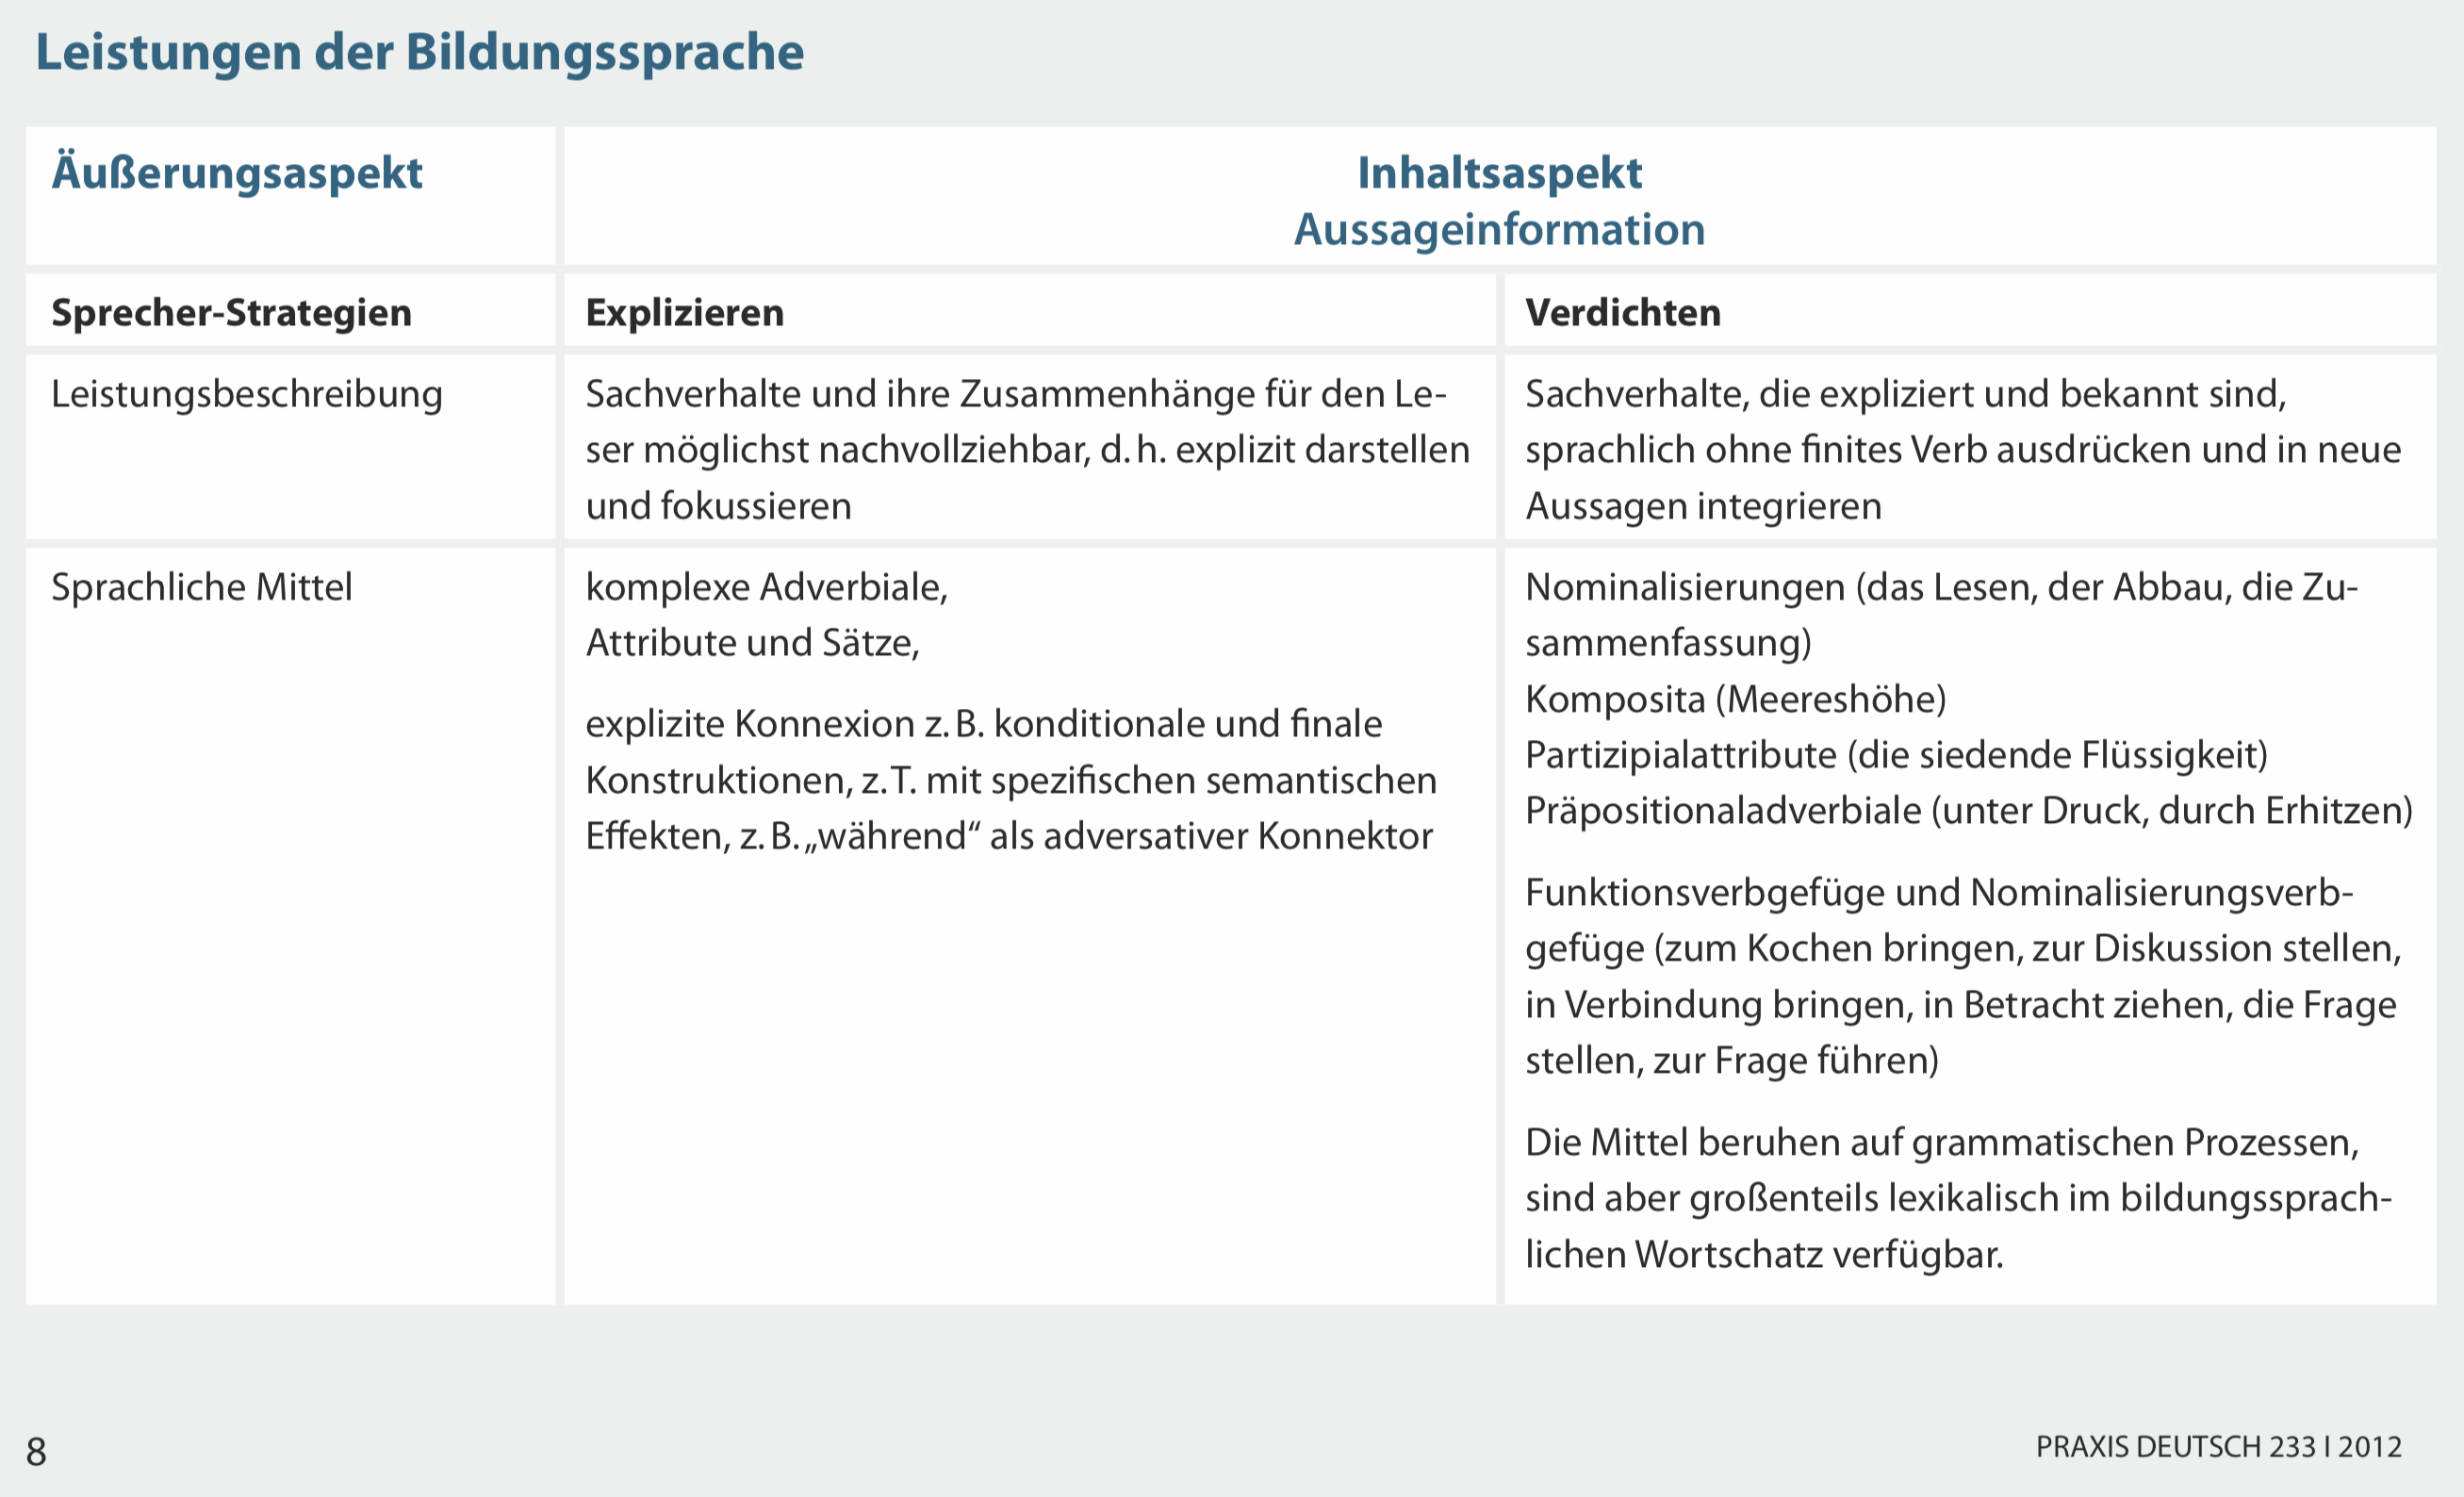
\includegraphics[width=0.9\textwidth]{graphics/feilke1}
\end{frame}


\begin{frame}
  {Übrigens: grammatische Mittel und Bildungssprache}
  \pause
  Aus \citet{Feilke2012}\\
  \Halbzeile
  \pause
  \centering
  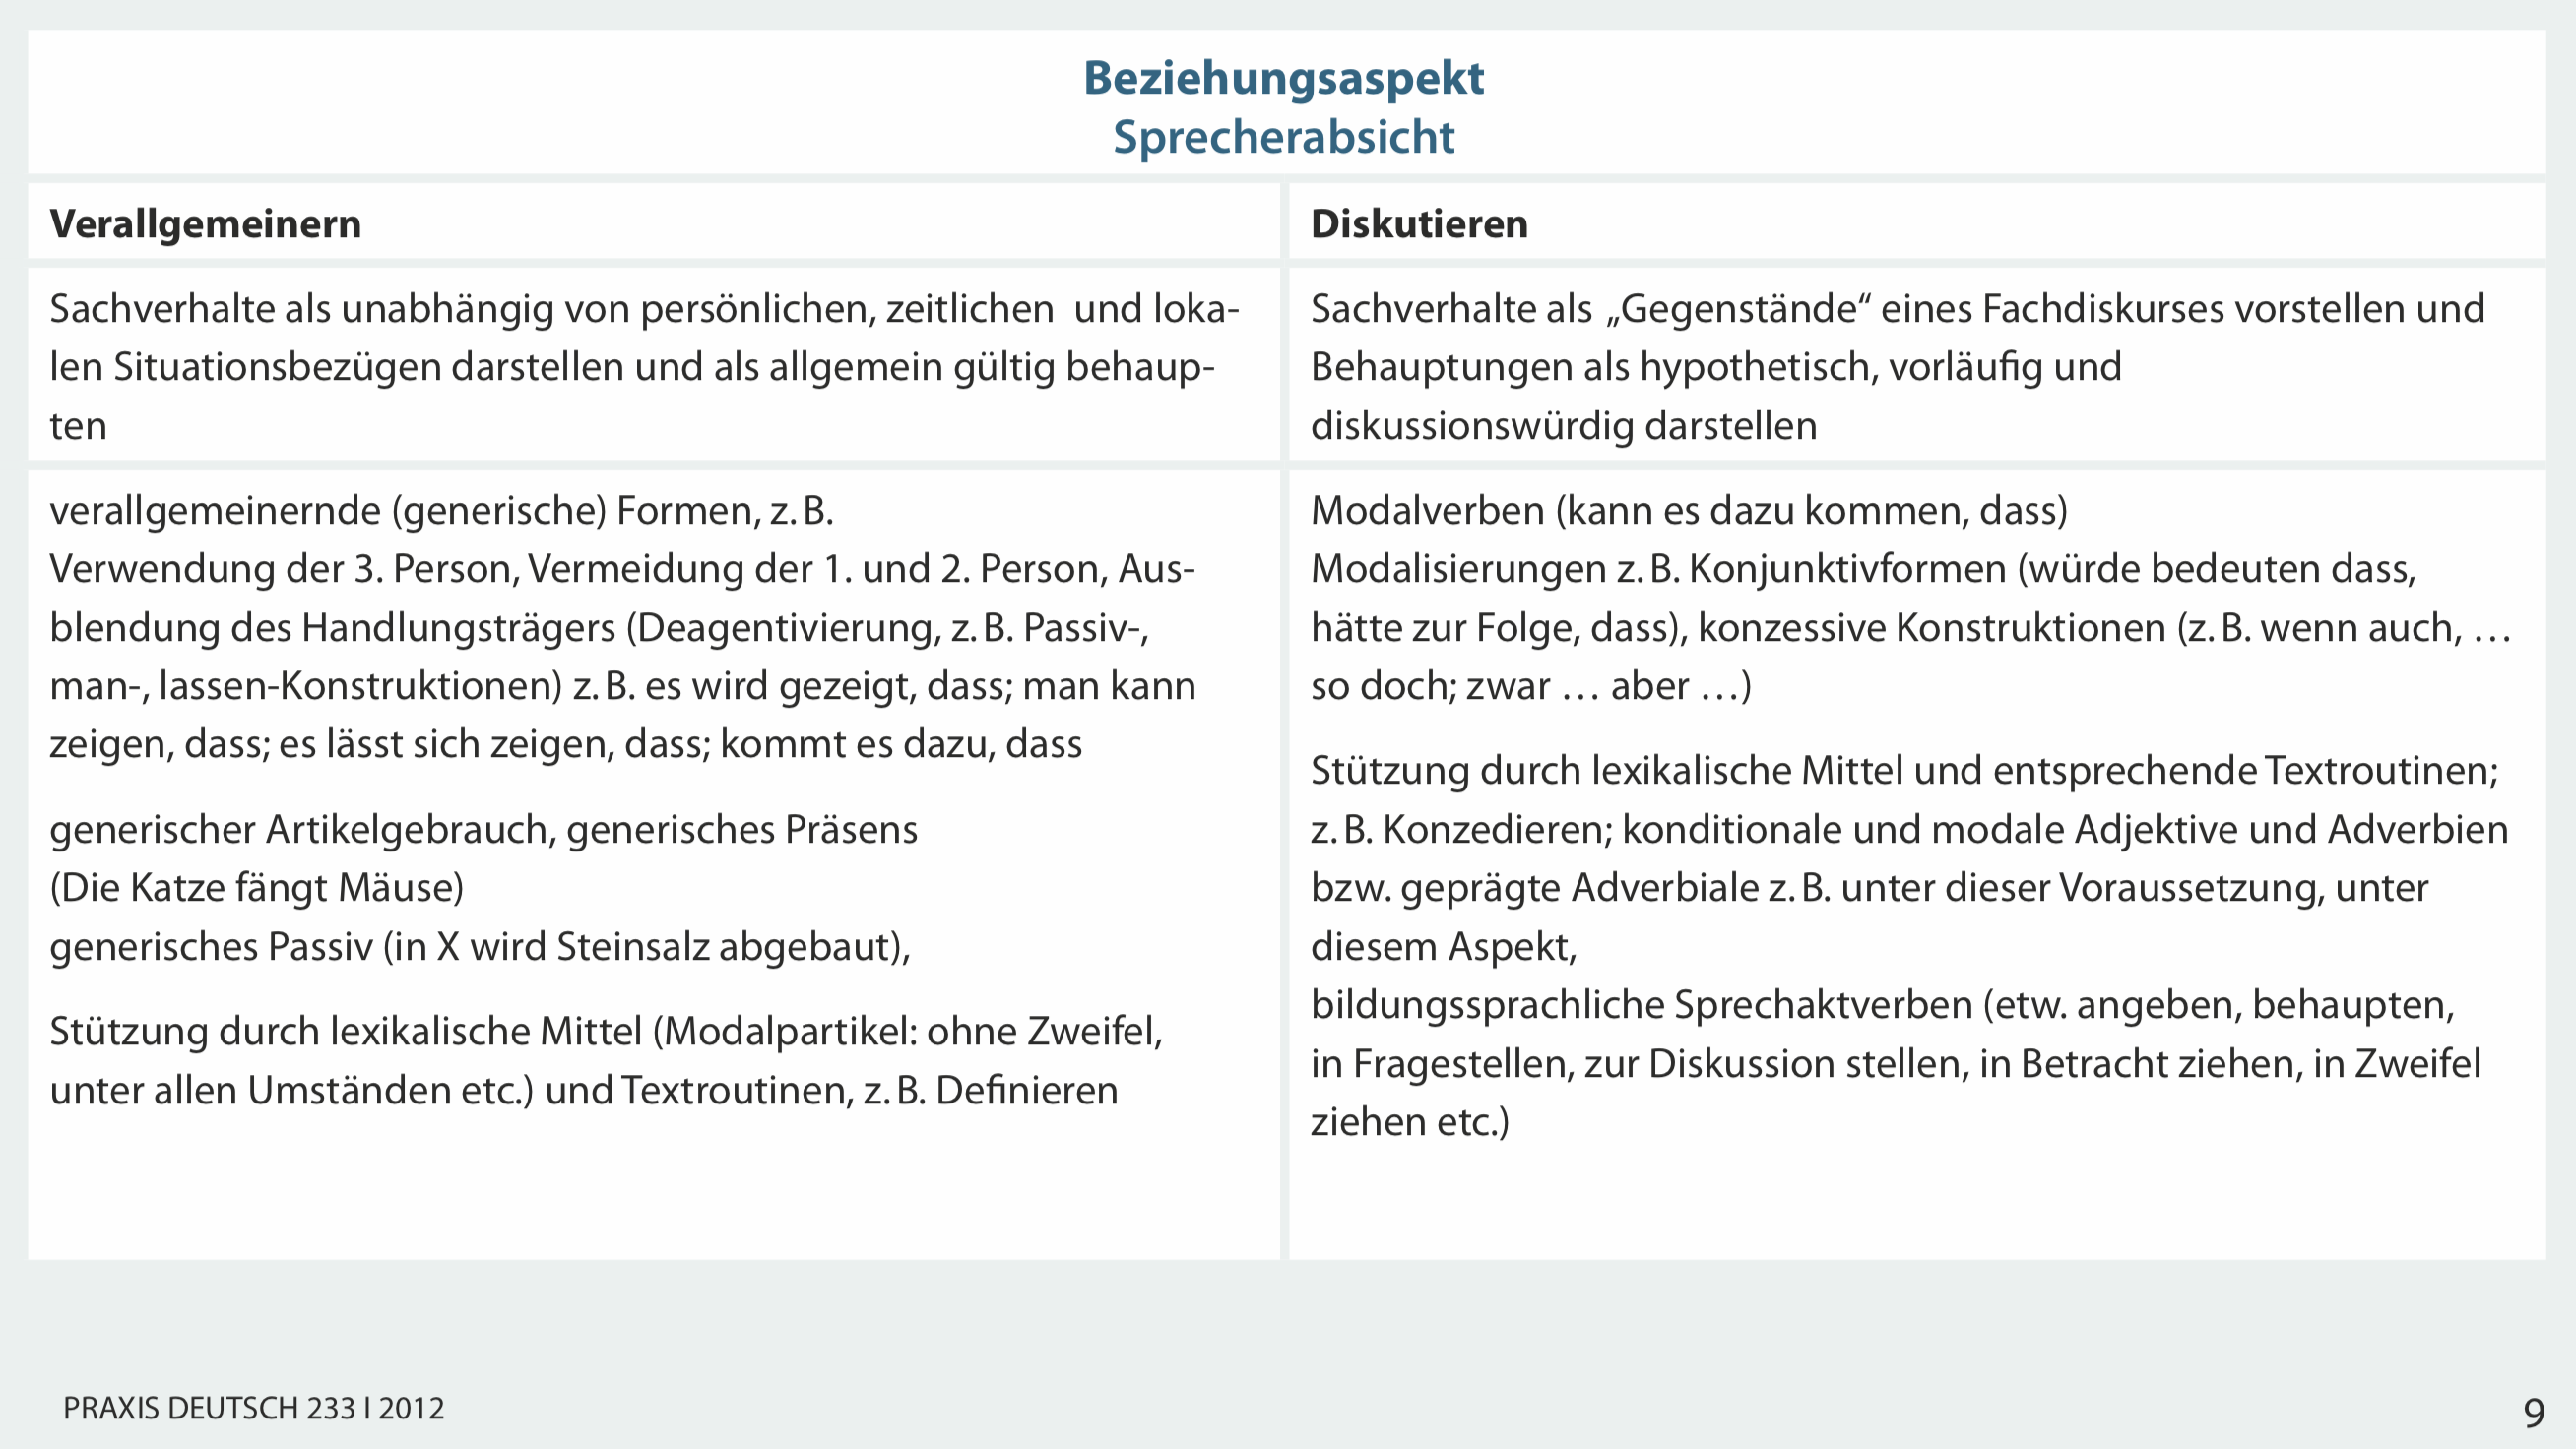
\includegraphics[width=0.9\textwidth]{graphics/feilke2}
\end{frame}


\section{Überblick}

\begin{frame}
  {Relationen und Prädikate}
  \pause
  \begin{itemize}[<+->]
    \item Verbsemantik und Valenz: semantische Rollen
      \Halbzeile
    \item Warum ist der Begriff \textit{Subjekt} überflüssig?
    \item Warum ist der Begriff \textit{Prädikat} problematisch?
    \item Wieviele Passive gibt es, und welche Verben sind passivierbar?
    \item Was sind direkte, indirekte und PP-Objekte?
    \item Und was sind Dativ- und PP-Angaben?
      \Halbzeile
    \item \alert{Valenzänderungen} und \alert{Valenzerweiterungen}
      \Halbzeile
    \item Gerade \alert{wegen} der Schwierigkeiten mit der Schulterminologie\\
      wird hier heute Wichtiges gelernt!
  \end{itemize}

\end{frame}

\begin{frame}
  {Relationen?}
  \pause
  \begin{itemize}[<+->]
    \item \alert{Kategorien}
      \begin{itemize}[<+->]
        \item Wortklasse?
        \item Numerus
        \item Tempus
        \item Komparationsstufe
        \item Kasus?
          \Halbzeile
        \item \alert{für die jeweilige Einheit definiert}
      \end{itemize}
      \Halbzeile
    \item \alert{Relationen}
      \begin{itemize}[<+->]
        \item Subjekt, Objekt (zum Verb)
        \item Ergänzung\slash Angabe (zu einem Wort)
        \item Prädikat (eines Satzes?)
        \item Attribut (zu einem Nomen)
          \Halbzeile
        \item \alert{zwischen Einheiten definiert}
        \item \alert{erfordern oft bestimmte Kategorien}
      \end{itemize}
  \end{itemize}
  \pause
  \Halbzeile
  \rot{Relationen helfen, syntaktische Strukturen zu dekodieren.}
\end{frame}

\section{Semantische Rollen}

\begin{frame}
  {Semantik-Grammatik-Schnittstelle}
  \pause
  \begin{exe}
    \ex
    \begin{xlist}
      \ex{\alert{Michelle} kauft einen Rottweiler.}
      \pause
      \ex{\alert{Der Rottweiler} schläft.}
      \pause
      \ex{\alert{Der Rottweiler} erfreut Marina.}
    \end{xlist}
  \end{exe}
  \pause
  \Halbzeile
  \begin{itemize}[<+->]
    \item semantische Generalisierung über \alert{Käuferin}, \alert{Schläfer}, \alert{Erfreuer}?
    \item \rot{"`Das Subjekt drückt aus, wer oder was im Satz handelt."'}
    \item Nur die \alert{Käuferin} handelt!
      \Halbzeile
    \item Verben als Kodierung eines \alert{Situationstyps} 
    \item Situationstypen mit charakteristischen \alert{Mitspielern}
    \item Handelnde, Betroffene, Veränderte, Emotionen Erfahrende, \ldots
    \item "`Mitspieler"' im weiteren Sinn, auch Gegenstände, Zeitpunkte usw.
      \Halbzeile
    \item Gleichsetzung von Rollen mit Kasūs: \rot{absoluter Unsinn}
  \end{itemize}
\end{frame}

\begin{frame}
  {Agens und Experiencer}
  \pause
  \begin{exe}
    \ex
    \begin{xlist}
      \ex{\alert{Michelle} kauft \orongsch{einen Rottweiler}.}
      \ex{\orongsch{Der Rottweiler} schläft.}
      \ex{\orongsch{Der Rottweiler} erfreut \rot{Marina}.}
    \end{xlist}
  \end{exe}
  \pause
  \Halbzeile
  \begin{itemize}[<+->]
    \item Rollen in den Beispielen
      \begin{itemize}[<+->]
        \item \alert{Michelle}: Handelnde = \alert{Agens}
        \item \rot{Marina}: psychischen Zustand Erfahrende: \rot{Experiencer}
        \item \orongsch{Rottweiler}: andere Rollen, hier nicht weiter analysiert (Rx)
      \end{itemize}
  \end{itemize}
\end{frame}

\begin{frame}
  {Rollenzuweisung\ldots\ und Ergänzungen und Angaben}
  \pause
  \begin{itemize}[<+->]
    \item für einen Situationstyp charakteristische Rollen?
      \Halbzeile
    \item (fast) \alert{immer} \zB
      \begin{itemize}[<+->]
        \item \alert{Zeitpunkt}
        \item \alert{Ort}
        \item \alert{Dauer}
      \end{itemize}
      \Halbzeile
    \item \alert{nicht immer} \zB
      \begin{itemize}[<+->]
        \item \rot{Handelnde} (\textit{schlafen}, \textit{fallen}, \textit{gefallen}, \ldots)
        \item \rot{psychischen Zustand Erfahrende} (\textit{laufen}, \textit{reparieren}, \textit{spinnen}, \ldots)
        \item \rot{Veränderte} (\textit{betrachten}, \textit{belassen}, \textit{verkaufe}, \ldots)
      \end{itemize}
      \Halbzeile
    \item Auch wenn Kaufen, Fallen usw.\ Emotionen auslöst:\\
      \alert{Das jeweilige Verb (\textit{kaufen}, \textit{fallen} usw.) sagt darüber nichts aus!}
      \Halbzeile
    \item \rot{Ergänzung}: gekoppelt an \alert{verbspezifische} Rolle 
    \item \alert{Angabe}: gekoppelt an \alert{verbunspezifische} Rolle
    \item erinnere: \textit{(nicht) subklassenspezifische Lizenzierung}
  \end{itemize}
\end{frame}

\begin{frame}
  {Das Prinzip der Rollenzuweisung}
  \pause
  \begin{itemize}[<+->]
    \item situationsspezifische Rollen: \alert{nur einmal vergebbar}\\
    = Prinzip der Rollenzuweisung
      \Halbzeile
    \item semantische Motivation für:
      \begin{itemize}[<+->]
        \item Angaben sind iterierbar,
        \item Ergänzungen nicht.
      \end{itemize}
      \Halbzeile
    \item und \alert{Koordinationen}?
  \end{itemize}
  \pause
  \begin{exe}
    \ex \alert{Marina und Michelle} kaufen bei \rot{einer seriösen Züchterin\\
    und ihrer Freundin} einen \orongsch{Dobermann und einen Rottweiler}.
  \end{exe}
  \pause
  \begin{itemize}[<+->]
    \item semantisch: Summenindividuen o.\,ä.
    \item \alert{Grammatik und Semantik untrennbar, gegenseitig bedingend}
  \end{itemize}
\end{frame}

\section{Subjekte}

\begin{frame}
  {Kernfrage: Brauchen wir den Begriff "`Subjekt"'?}
  \pause
  \textit{"`In jedem vollständigen Satz wird das Prädikat durch das Subjekt ergänzt. Das Subjekt nennt die Person oder die Sache, von der das Geschehen ausgeht, oder zu der ein Zustand gehört."'}\\
  \pause\Viertelzeile
  {\small (Mein Übungsbuch: Grammatik Deutsch im Griff 5.\slash 6.~Klasse, Klett 2018, S.~93)}
  \pause
  \Halbzeile
  \begin{itemize}[<+->]
    \item Na, was sagen wir denn dazu?
      \begin{itemize}[<+->]
        \item \rot{Wetter-Verben}?
        \item \rot{Passivsätze}?
        \item \rot{Subjektsätze}?
        \item \ldots um nur einige der wichtigsten Probleme zu nennen.
      \end{itemize}
  \end{itemize}
\end{frame}

\begin{frame}
  {Potentielle Subjekte: Wo wollen wir denn hin?}
  \pause
  \begin{exe}
    \ex
    \begin{xlist}
      \ex[ ]{\alert{[Frau Brüggenolte]} backt einen Kuchen.}
      \ex[*]{Backt einen Kuchen.}
      \pause
      \ex[ ]{\alert{[Herr Uhl]} raucht.}
      \ex[*]{Raucht.}
      \pause
      \ex[ ]{\alert{[Es]} regnet.}
      \ex[*]{Regnet.}
      \pause
      \ex[ ]{\alert{[Dass Herr Oelschlägel jeden Tag staubsaugt]}, nervt Herrn Uhl.}
      \ex[*]{Nervt Herrn Uhl.}
      \pause
      \ex[ ]{\alert{[Zu Fuß den Fahrstuhl zu überholen]}, machte mir als Kind Spaß.}
      \ex[*]{Machte mir als Kind Spaß.}
      \pause
      \ex[ ]{Es friert mich.}
      \ex[ ]{Mich friert. \onslide<7->{\rot{Ups!}}}
    \end{xlist}
  \end{exe}
  \pause
  \begin{itemize}[<+->]
    \item lauter regierte obligatorische Ergänzungen
    \item \alert{Was ist denen gemein?}
  \end{itemize}
\end{frame}

\begin{frame}
  {Subjekte = verbregierte kongruierende Nominative}
  \pause
  \begin{itemize}[<+->]
    \item Was wird denn so alles "`Subjekt"' genannt?
      \begin{itemize}[<+->]
        \item \alert{regierte Nominative}
        \item \alert{die mit dem Verb kongruieren}
        \item oder \alert{Nebensätze} an der Stelle solcher Nominative
        \item \grau{Achtung: Nebensätze haben keine Kongruenzmerkmale\\
            und keinen Kasus! Subjektsätze sind nicht \textit{3.~Person Nominativ}.}
      \end{itemize}
      \Halbzeile
    \item \rot{Das wars. Nichts mit "`Satzgegenstand"', "`Handelnde"' usw.}
      \Halbzeile
    \item Brauchen wir den Begriff dann?
      \begin{itemize}[<+->]
        \item \alert{eigentlich überflüssig}
        \item \ldots aber ganz praktisch als Abkürzung
          \Halbzeile
        \item \rot{Durch die schulische Vermittlung des Begriffs ist\\
          keine Verbesserung der bildungssprachlichen Fähigkeiten zu erwarten.}
      \end{itemize}
  \end{itemize}
  \pause
\end{frame}

\begin{frame}
  {\textit{Es} ist nicht, was es scheint.}
  \pause
  \begin{exe}
    \ex
    \begin{xlist}
      \ex{\alert<4->{Es} öffnet die Tür.}
      \ex{\rot<4->{Es} regt mich auf, dass die Politik schon wieder versagt.}
      \ex{\rot<4->{Es} öffnet ein Kind die Tür.}
      \ex{\rot<4->{Es} wird jetzt gearbeitet.}
      \ex{\rot<4->{Es} friert mich.}
      \ex{\rot<4->{Es} regnet in Strömen.}
    \end{xlist}
  \end{exe}
  \pause
  \begin{itemize}[<+->]
    \item Ersetzbar durch Vollpronomen (\zB\ \textit{dieses})?
    \item \alert{Subjektpronomen}
  \end{itemize}
\end{frame}

\begin{frame}
  {\textit{Es} ist nicht, was es scheint.}
  \begin{exe}
    \ex
    \begin{xlist}
      \ex{\grau{Es öffnet die Tür.}}
      \ex{\alert<3->{Es} regt mich auf, dass die Politik schon wieder versagt.}
      \ex{\rot<3->{Es} öffnet ein Kind die Tür.}
      \ex{\rot<3->{Es} wird jetzt gearbeitet.}
      \ex{\rot<3->{Es} friert mich.}
      \ex{\rot<3->{Es} regnet in Strömen.}
    \end{xlist}
  \end{exe}
  \pause
  \begin{itemize}[<+->]
    \item Tritt auf und korreliert mit Subjektsatz?
    \item \alert{Korrelat}
  \end{itemize}
\end{frame}

\begin{frame}
  {\textit{Es} ist nicht, was es scheint.}
  \begin{exe}
    \ex
    \begin{xlist}
      \ex{\grau{Es öffnet die Tür.}}
      \ex{\grau{Es regt mich auf, dass die Politik schon wieder versagt.}}
      \ex{\alert<4->{Es} öffnet ein Kind die Tür.}
      \ex{\alert<4->{Es} wird jetzt gearbeitet.}
      \ex{\rot<4->{Es} friert mich.}
      \ex{\rot<4->{Es} regnet in Strömen.}
    \end{xlist}
  \end{exe}
  \pause
  \begin{itemize}[<+->]
    \item Immer in Satz-Erst-Position (\textit{Vorfeld})?
    \item \ldots und immer weglassbar
    \item \alert{positionales \textit{Es}} oder \alert{Vorfeld-\textit{Es}}
    \item reiner Vorfeld-Füller
  \end{itemize}
\end{frame}

\begin{frame}
  {\textit{Es} ist nicht, was es scheint.}
  \begin{exe}
    \ex
    \begin{xlist}
      \ex{\grau{Es öffnet die Tür.}}
      \ex{\grau{Es regt mich auf, dass die Politik schon wieder versagt.}}
      \ex{\grau{Es öffnet ein Kind die Tür.}}
      \ex{\grau{Es wird jetzt gearbeitet.}}
      \ex{\alert<3->{Es} friert mich.}
      \ex{\orongsch<4->{Es} regnet in Strömen.}
    \end{xlist}
  \end{exe}
  \pause
  \begin{itemize}[<+->]
    \item Optional?
    \item Ja: \alert{fakultative Ergänzung bei \textit{Experiencer}-Verben}
    \item Nein: \orongsch{obligatorische Ergänzung bei \textit{Wetter}-Verben}
      \Halbzeile
    \item Achtung: Die Ergänzung ist hier absolut festgelegt auf \textit{es}!
    \item Es wird nicht nur der Kasus oder die PP-Form regiert.
  \end{itemize}
\end{frame}


\section{Prädikate}

\begin{frame}
  {"`Satzprädikat"'?}
  \pause
  \textit{"`Jeder vollständige Satz besitzt (sic!) ein Prädikat. Es drückt aus, was im Satz geschieht oder ist. Das Prädikat ist der wichtigste Bestandteil eines Satzes. Von ihm hängen die anderen Bausteine des Satzes ab. [\ldots] Das Prädikat ist immer eine konjugierte Verbform."'}\\
  \pause\Viertelzeile
  {\small (Mein Übungsbuch: Grammatik Deutsch im Griff 5.\slash 6.~Klasse, Klett 2018, S.~90)}
  \pause
  \Halbzeile
  \begin{itemize}[<+->]
    \item \rot{Unterschied zwischen \textit{Prädikat} und \textit{finites Verb}?}
    \item analytische Verbformen (\textit{geklebt haben durfte})?
    \item "`was geschieht oder ist"'? -- \textit{Chloë spielt Tennis.}
    \item OK, vielleicht ohne Subjekt? -- \textit{spielt Tennis.}
      \Halbzeile
    \item \textit{Prädikat} ist ein \alert{semantischer Begriff} (s.~\textit{Prädikatenlogik})\ldots
    \item \ldots der \alert{in der Schulgrammatik nichts zu suchen hat}.
  \end{itemize}
\end{frame}

\begin{frame}
  {"`Prädikativergänzungen"'}
  \pause
  Andere \textit{prädikative} Konstituenten außer dem \textit{Satzprädikat}?\\
  \Halbzeile
  \begin{exe}
    \ex\label{ex:praedikative022}
    \begin{xlist}
      \ex{\label{ex:praedikative023} Stig wird [gesund].}
      \pause
      \ex{\label{ex:praedikative024} Stig bleibt [ein Arzt].}
      \pause
      \ex{\label{ex:praedikative025} Stig ist, [wie er ist].}
      \pause
      \ex{\label{ex:praedikative026} Stig ist [in Kopenhagen].}
    \end{xlist}
  \end{exe}
  \pause
  \Halbzeile
  \begin{itemize}[<+->]
    \item \alert{Prädikativergänzung} bei Kopulaverben
    \item besser \rot{nicht \textit{Prädikatsnomen}} (s.~w-Satz und PP)
    \item Nominative (\textit{ein Arzt}): keine Kongruenz
  \end{itemize}
\end{frame}

\begin{frame}
  {Resultativprädikate}
  \pause
  Sind das "`Adverben"' oder "`Adverbiale"'\ldots oder was?\\
  \Halbzeile
  \pause
  \begin{exe}
    \ex\label{ex:praedikative027}
    \begin{xlist}
      \ex{\label{ex:praedikative028} Er fischt den Teich [leer].
      \onslide<5->{\alert{→ Der Teich wird [leer].}}}
      \ex{\label{ex:praedikative029} Sie färbt den Pullover [grün].
      \onslide<5->{\alert{→ Der Pullover wird [grün].}}}
      \ex{\label{ex:praedikative030} Er stampft die Äpfel [zu Brei].
      \onslide<5->{\alert{→ Die Äpfel werden [zu Brei].}}}
    \end{xlist}
  \end{exe}
  \pause
  \begin{itemize}[<+->]
    \item Als \alert{"`[NP] ist\slash wird [Kopula]."'} formulierbar?
    \item \alert{Ja! Ähnlichkeit zu Prädikativergänzungen bei Kopulaverben.}
    \item "`Resultativprädikate"'?\ldots Meinethalber.
    \item keine einfachen Angaben wegen \rot{Valenzänderung}
    \item also \rot{keine} "`Adverben"', "`adverbiale Bestimmungen"' usw.
  \end{itemize}
\end{frame}

\begin{frame}
  {"`Prädikativergänzungen"'?}
  \pause
  Sind das "`Prädikative"' oder gar "`Prädikatsnomina"'?\\
  \Halbzeile
  \pause
  \begin{exe}
    \ex\label{ex:praedikative032}
    \begin{xlist}
      \ex{\label{ex:praedikative033} Ich halte den Begriff [für unnütz].\\
        \onslide<5->{\rot{→ *Der Begriff ist/wird [für unnütz].}}}
      \ex{\label{ex:praedikative034} Sie gelten bei mir [als Langweiler].\\
        \onslide<5->{\rot{→ *Sie sind/werden [als Langweiler].}}}
      \ex{\label{ex:praedikative035} Das Eis schmeckt [toll].
        \onslide<5->{\rot{→ *Das Eis ist/wird [toll].}}}
    \end{xlist}
  \end{exe}
  \pause
  \begin{itemize}[<+->]
    \item Funktioniert der Kopula-Test?
    \item \rot{Nein! Keine Ähnlichkeit zur Kopulativ-Ergänzung.}
    \item \alert{Form vom Verb vorgegeben}, also:
      \begin{itemize}[<+->]
        \item \textit{für}-PP-Ergänzung (\textit{halten})
        \item \textit{als}-PP(?)-Ergänzung (\textit{gelten})
        \item Adjektiv-Ergänzung (\textit{schmecken}\ldots)\\
          \grau{(Oder Angabe? Siehe evtl.\ Vertiefung~2.2, S.~46.)}
      \end{itemize}
  \end{itemize}
\end{frame}


\section{Passivbildungen}

\begin{frame}[allowframebreaks]
  {\textit{werden}-Passiv oder Vorgangspassiv}
  \pause
  "`Nur transitive Verben können passiviert werden."'\pause\rot{--- Nein!}
  \pause
    \begin{exe}
    \addtolength\itemsep{-0.25\baselineskip}
      \ex\label{ex:werdenpassivundverbtypen110}
      \begin{xlist}\addtolength\itemsep{-0.5\baselineskip}
          \ex[ ]{\label{ex:werdenpassivundverbtypen111} \alert{Johan} wäscht \orongsch{den Wagen}.}
          \ex[ ]{\label{ex:werdenpassivundverbtypen112} \orongsch{Der Wagen} wird \alert{(von Johan)} gewaschen.}
      \end{xlist}
      \pause
      \ex\label{ex:werdenpassivundverbtypen113}
      \begin{xlist}\addtolength\itemsep{-0.5\baselineskip}
          \ex[ ]{\label{ex:werdenpassivundverbtypen114} \alert{Alma} schenkt \gruen{dem Schlossherrn} \orongsch{den Roman}.}
          \ex[ ]{\label{ex:werdenpassivundverbtypen115} \orongsch{Der Roman} wird \gruen{dem Schlossherrn} \alert{(von Alma)} geschenkt.}
      \end{xlist}
      \pause
      \ex\label{ex:werdenpassivundverbtypen116}
      \begin{xlist}\addtolength\itemsep{-0.5\baselineskip}
          \ex[ ]{\label{ex:werdenpassivundverbtypen117} \alert{Johan} bringt \orongsch{den Brief} zur Post.}
          \ex[ ]{\label{ex:werdenpassivundverbtypen118} \orongsch{Der Brief} wird \alert{(von Johan)} zur Post gebracht.}
      \end{xlist}
      \pause
      \ex\label{ex:werdenpassivundverbtypen119}
      \begin{xlist}\addtolength\itemsep{-0.5\baselineskip}
          \ex[ ]{\label{ex:werdenpassivundverbtypen120} \alert{Der Maler} dankt \gruen{den Fremden}.}
          \ex[ ]{\label{ex:werdenpassivundverbtypen121} \gruen{Den Fremden} wird \alert{(vom Maler)} gedankt.}
      \end{xlist}
      \pause
      \ex\label{ex:werdenpassivundverbtypen122}
      \begin{xlist}\addtolength\itemsep{-0.5\baselineskip}
          \ex[ ]{\label{ex:werdenpassivundverbtypen123} \alert{Johan} arbeitet hier immer montags.}
          \ex[ ]{\label{ex:werdenpassivundverbtypen124} Montags wird hier \alert{(von Johan)} immer gearbeitet.}
      \end{xlist}
      \pause
      \ex\label{ex:werdenpassivundverbtypen125}
      \begin{xlist}\addtolength\itemsep{-0.5\baselineskip}
          \ex[ ]{\label{ex:werdenpassivundverbtypen126} \alert{Der Ball} platzt bei zu hohem Druck.}
          \ex[*]{\label{ex:werdenpassivundverbtypen127} Bei zu hohem Druck wird \rot{(vom Ball)} geplatzt.}
      \end{xlist}
      \pause
      \ex\label{ex:werdenpassivundverbtypen128}
      \begin{xlist}\addtolength\itemsep{-0.5\baselineskip}
          \ex[ ]{\label{ex:werdenpassivundverbtypen129} \alert{Der Rottweiler} fällt \gruen{Michelle} auf.}
          \ex[*]{\label{ex:werdenpassivundverbtypen130} \alert{Michelle} wird \rot{(von dem Rottweiler)} aufgefallen.}
      \end{xlist}
    \end{exe}
\end{frame}

\begin{frame}
  {Was passiert beim Vorgangspassiv?}
  \pause
  \begin{itemize}[<+->]
    \item Auxiliar: \textit{werden}, Verbform: Partizip
    \item für Passivierbarkeit relevant: \alert{die Nominativ-Ergänzung!}
      \Halbzeile
    \item \alert{Passivierung = Valenzänderung}:
      \begin{itemize}[<+->]
        \item Nominativ-Ergänzung → optionale \textit{von}-PP-Angabe
        \item eventuelle Akkusativ-Ergänzung → obligatorische Nominativ-Ergänzung
        \item kein Akkusativ: kein "`Subjekt"' = keine Nom-Erg (\textit{es} ist positional)
        \item \grau{Dativ-Ergänzung → Dativ-Ergänzung (usw.)}
        \item \grau{Angaben: keine Änderung}
      \end{itemize}
    \Halbzeile
  \item \alert{nicht passivierbare Verben}?
    \begin{itemize}[<+->]
      \item {ohne }\rot{agentivische}\alert{ Nominativ-Ergänzung}
      \item Achtung! Gilt nur mit prototypischem Charakter\ldots
      \item Siehe Vertiefung 14.2 auf S.~439!
    \end{itemize}
  \end{itemize}
\end{frame}

\begin{frame}
  {Feinere Klassifikation von Verben}
  \pause
  \begin{itemize}[<+->]
    \item Neuklassifikation vor dem Hintergrund des Vorgangspassivs
    \item Wenn so eine Klassifikation einen Wert haben soll:\\
      \alert{Berücksichtigung der semantischen Rollen unabdinglich!}
    \item Bedingung für Vorgangs-Passiv: \alert{Nom\_Ag}
  \end{itemize} 
  \pause
  \Zeile
  \centering
  \begin{tabular}{lllll}
    \toprule
    \textbf{Valenz} & \textbf{Passiv} & \textbf{Name} & \textbf{Beispiel} \\
    \midrule
    \alert{Nom\_Ag} & ja & Unergative & \textit{arbeiten} \\
    Nom & nein & Unakkusative & \textit{platzen} \\
    \alert{Nom\_Ag}, Akk & ja & Transitive & \textit{waschen} \\
    \alert{Nom\_Ag}, Dat & ja & unergative Dativverben & \textit{danken} \\
    Nom, Dat & nein & unakkusative Dativverben & \textit{auf"|fallen} \\
    \alert{Nom\_Ag}, Dat, Akk & ja & Ditransitive & \textit{geben} \\
    \bottomrule
  \end{tabular}\\
  \raggedright
  \Zeile
  \pause
  Immer noch nichts als eine reine Bequemlichkeitsterminologie,\\
  um bestimmte (durchaus wichtige) Valenzmuster hervorzuheben.
\end{frame}


\begin{frame}
  {\textit{bekommen}-Passiv oder Rezipientenpassiv}
  \pause
  Es gibt nicht "`das Passiv im Deutschen"'.\\
  \Halbzeile
  \pause
  \begin{exe}
    \ex\label{ex:bekommenpassiv138}
    \begin{xlist}
      \ex[ ]{\small\label{ex:bekommenpassiv139} \gruen{Mein Kollege} bekommt \orongsch{den Wagen} \alert{(von Johan)} gewaschen.}
      \pause
      \ex[ ]{\small\label{ex:bekommenpassiv140} \gruen{Der Schlossherr} bekommt \orongsch{den Roman} \alert{(von Alma)} geschenkt.}
      \pause
      \ex[ ]{\small\label{ex:bekommenpassiv141} \gruen{Mein Kollege} bekommt \orongsch{den Brief} \alert{(von Johan)} zur Post gebracht.}
      \pause
      \ex[ ]{\small\label{ex:bekommenpassiv142} \gruen{Die Fremden} bekommen \alert{(von dem Maler)} gedankt.}
      \pause
      \ex[?]{\small\label{ex:bekommenpassiv143} \gruen{Mein Kollege} bekommt hier immer montags \alert{(von Johan)} gearbeitet.}
      \pause
      \ex[*]{\small\label{ex:bekommenpassiv144} \gruen{Mein Kollege} bekommt bei zu hohem Druck \rot{(von dem Ball)} geplatzt.}
      \pause
      \ex[*]{\small\label{ex:bekommenpassiv145} \gruen{Michelle} bekommt \rot{(von dem Rottweiler)} aufgefallen.}
    \end{xlist}
  \end{exe}
  \pause\Halbzeile
  \alert{Das ist eine Passivbildung, die genauso den Nom\_Ag betrifft\\
  wie das Vorgangspassiv.}
\end{frame}

\begin{frame}
  {Was passiert beim Rezipientenpassiv?}
  \pause
  Alles, was sich verglichen mit Vorgangspassiv nicht unterscheidet, grau.\\
  \Halbzeile
  \pause
  \begin{itemize}[<+->]
    \item Auxiliar: \textit{bekommen} (evtl.\ \textit{kriegen}), \grau{Verbform: Partizip}
    \item \grau{für Passivierbarkeit relevant: die Nominativ-Ergänzung!}
      \Halbzeile
    \item \grau{Passivierung = Valenzänderung}:
      \begin{itemize}[<+->]
        \item \grau{Nominativ-Ergänzung → optionale \textit{von}-PP-Angabe}
        \item eventuelle Akkusativ-Ergänzung: → Akkusativ-Ergänzung
        \item \alert{Dativ-Ergänzung → Nominativ-Ergänzung}
        \item \rot{kein Dativ: kein Rezipientenpassiv}
        \item \grau{Angaben: keine Änderung}
      \end{itemize}
    \Halbzeile
  \item \grau{nicht passivierbare Verben?}
    \begin{itemize}[<+->]
      \item \grau{ohne agentivische Nominativ-Ergänzung}
      \item \grau{Achtung! Gilt nur mit prototypischem Charakter\ldots}
      \item \grau{Siehe Vertiefung 14.2 auf S.~439!}
    \end{itemize}
  \end{itemize}
\end{frame}

\begin{frame}
  {Rezipientenpassiv bei unergativen Verben}
  \pause
  Warum war dieser Satz zweifelhaft?\\
  \begin{exe}
    \ex[?]{\small \gruen{Mein Kollege} bekommt hier immer montags \alert{(von Johan)} gearbeitet.}
  \end{exe}
  \pause
  \Halbzeile
  Ist der zugehörige Aktivsatz besser?\\
  \pause
  \begin{exe}
    \ex[?]{\small Montags arbeitet \alert{Johan} \gruen{meinem Kollegen} hier immer.}
  \end{exe}
  \pause
  \begin{itemize}[<+->]
    \item Nein.
    \item \alert{keine Frage des Rezipientenpassivs}
    \item bei diesen Verben: eher \textit{für}-PP
  \end{itemize}
\end{frame}


\section{Objekte und Valenz}

\begin{frame}
  {Direkte Objekte}
  \pause
   Kaum anders als beim Subjekt.
  \begin{itemize}[<+->]
    \item \alert{Akkusativ-Ergänzungen zum Verb}
    \item \alert{oder Nebensätze an deren Stelle}
  \end{itemize}
  \pause
  \Halbzeile
  Und Doppelakkusative?\\
  \begin{exe}
    \ex\label{ex:akkusativeunddirekteobjekte158}
    \begin{xlist}
      \ex[ ]{\label{ex:akkusativeunddirekteobjekte159} Ich lehre \alert{ihn} \orongsch{das Schwimmen}.}
      \pause
      \ex[*]{\label{ex:akkusativeunddirekteobjekte160} \orongsch{Das Schwimmen} wird \alert{ihn} gelehrt.}
      \pause
      \ex[*]{\label{ex:akkusativeunddirekteobjekte161} \alert{Er} wird \orongsch{das Schwimmen} gelehrt.}
      \pause
      \ex[ ]{\label{ex:akkusativeunddirekteobjekte161} Hier wird \orongsch{das Schwimmen} gelehrt.}
    \end{xlist}
  \end{exe}
  \pause
  \begin{itemize}[<+->]
    \item unterschiedlicher Status der Akkusativ-Ergänzungen
    \item Die "`erste"' entspricht der normaler Transitiva.
    \item \grau{Korrektur zum Buch: Doppelakkusative bilden unpersönliche Passive.}
  \end{itemize} 
\end{frame}

\begin{frame}
  {Indirekte Objekte}
  \pause
  Welche Dative sind Ergänzungen (= Teil der Valenz)?\\
  \pause
  \Halbzeile
  \begin{exe}
    \ex\label{ex:dativeundindirekteobjekte166}
    \begin{xlist}
      \ex[ ]{\label{ex:dativeundindirekteobjekte167} \alert{Alma} gibt \gruen{ihm} heute ein Buch.}
      \pause
      \ex[ ]{\label{ex:dativeundindirekteobjekte168} \alert{Alma} fährt \gruen{mir} heute aber wieder schnell.}
      \pause
      \ex[ ]{\label{ex:dativeundindirekteobjekte169} \alert{Alma} mäht \gruen{mir} heute den Rasen.}
      \pause
      \ex[ ]{\label{ex:dativeundindirekteobjekte170} \alert{Alma} klopft \gruen{mir} heute auf die Schulter.}
    \end{xlist}
  \end{exe}
  \Halbzeile
  \pause
  Recht einfache Entscheidung, da wir Passiv\\
  als \alert{Valenzänderung} beschreiben:\\
  \pause
  \begin{exe}
    \ex\label{ex:dativeundindirekteobjekte171}
    \begin{xlist}
      \ex[ ]{\label{ex:dativeundindirekteobjekte172} \gruen{Er} bekommt \alert{von Alma} heute ein Buch gegeben.}
      \ex[*]{\label{ex:dativeundindirekteobjekte173} \rot{Ich} bekomme \alert{von Alma} heute aber wieder schnell gefahren.}
      \ex[ ]{\label{ex:dativeundindirekteobjekte174} \gruen{Ich} bekomme \alert{von Alma} heute den Rasen gemäht.}
      \ex[ ]{\label{ex:dativeundindirekteobjekte175} \gruen{Ich} bekomme \alert{von Alma} heute auf die Schulter geklopft.}
    \end{xlist}
  \end{exe}
\end{frame}

\begin{frame}
  {Die vier wichtigen verbabhängigen Dative}
  \pause
  \begin{exe}
    \ex\label{ex:dativeundindirekteobjekte166x}
    \begin{xlist}
      \ex{\label{ex:dativeundindirekteobjekte167x} \alert{Alma} gibt \gruen{ihm} heute ein Buch.}
      \pause
      \ex{\label{ex:dativeundindirekteobjekte168x} \alert{Alma} fährt \gruen{mir} heute aber wieder schnell.}
      \pause
      \ex{\label{ex:dativeundindirekteobjekte169x} \alert{Alma} mäht \gruen{mir} heute den Rasen.}
      \pause
      \ex{\label{ex:dativeundindirekteobjekte170x} \alert{Alma} klopft \gruen{mir} heute auf die Schulter.}
    \end{xlist}
  \end{exe}
  \Halbzeile
  \pause
  \begin{itemize}[<+->]
    \item (\ref{ex:dativeundindirekteobjekte167x}) = gewöhnlicher Dativ bei ditransitivem Verb (Ergänzung)
      \Halbzeile
    \item (\ref{ex:dativeundindirekteobjekte168x}) = \gruen{Bewertungsdativ} (Angabe, steht immer direkt nach finiten Verb)
    \item (\ref{ex:dativeundindirekteobjekte169x}) = \gruen{Nutznießerdativ} (Ergänzung \alert{per Valenzerweiterung})
    \item (\ref{ex:dativeundindirekteobjekte170x}) = \gruen{Pertinenzdativ} (Ergänzung \alert{per Valenzerweiterung})
      \Halbzeile
    \item Bewertungsdativ, Nutznießerdativ und Pertinenzdativ\\
      nennt man auch \textit{freie Dative}.
  \end{itemize}
\end{frame}

\begin{frame}
  {Valenzveränderungen im Beispiel}
  \pause
  1.~Wir beginnen mit einem Verb mit \alert{Nom\_Ag} und einem \orongsch{Akk}:\\
  \pause
  \Halbzeile
  \begin{exe}
    \ex \alert{Alma} mäht \orongsch{den Rasen}.
  \end{exe}
  \Zeile
  \pause
  2.~Der \gruen{Nutznießerdativ} wird als Valenzerweiterung hinzugefügt:\\
  \pause
  \Halbzeile
  \begin{exe}
    \ex \alert{Alma} mäht \gruen{meinem Kollegen} \orongsch{den Rasen}.
  \end{exe}
  \Zeile
  \pause
  3.~Das Rezipientenpassiv (Valenzänderung) kann jetzt gebildet werden:
  \pause
  \Halbzeile
  \begin{exe}
    \ex \gruen{Mein Kollege} bekommt \alert{(von Alma)} \orongsch{den Rasen} gemäht.
  \end{exe}
\end{frame}

\begin{frame}
  {Präpositionalobjekte}
  \pause
  PP-Angabe vs.\ PP-Ergänzung: oft schwierig zu entscheiden.\\
  \Halbzeile
  \pause
  \begin{exe}
    \ex\label{ex:ppergaenzungenundppangaben189}
    \begin{xlist}
      \ex{\label{ex:ppergaenzungenundppangaben190} Viele Menschen leiden \alert{unter Vorurteilen}.}
      \pause
      \ex{\label{ex:ppergaenzungenundppangaben191} Viele Menschen schwitzen \orongsch{unter Sonnenschirmen}.}
    \end{xlist}
  \end{exe}
  \Halbzeile
  \pause
  \begin{itemize}[<+->]
    \item \alert{Ergänzungen}:
      \begin{itemize}[<+->]
        \item Semantik der PP nur verbgebunden interpretierbar
        \item = semantische Rolle der PP vom Verb zugewiesen
      \end{itemize}
      \Halbzeile
    \item \orongsch{Angaben}:
      \begin{itemize}[<+->]
        \item Semantik der PP selbständig erschließbar (lokal unter)
        \item = semantische Rolle der PP von der Präposition zugewiesen
      \end{itemize}
      \Halbzeile
    \item \alert{Sehen Sie, wie schnell man in der (Grund-)Schulgrammatik\\
      in gefährliche linguistische Fahrwasser gerät?}
    \item \rot{Wenn Sie dieses Wissen nicht haben, unterrichten Sie sehr leicht\\
      komplett Falsches, zumal wenn es im Lehrbuch falsch steht.}
  \end{itemize}
\end{frame}


\begin{frame}
  {Der umstrittene PP-Angaben-Test}
  \pause
  Die PP mit \textit{"`Dies geschieht PP."'} aus dem Satz auskoppeln.\\
  \Halbzeile
  \pause
  \begin{exe}
    \ex\label{ex:ppergaenzungenundppangaben192}
    \begin{xlist}
      \ex[*]{\label{ex:ppergaenzungenundppangaben193} Viele Menschen leiden.
      \rot{Dies geschieht unter Vorurteilen.}}
        \pause
      \ex[ ]{\label{ex:ppergaenzungenundppangaben194} Viele Menschen schwitzen.
      \alert{Dies geschieht unter Sonnenschirmen.}}
        \pause
      \ex[*]{\label{ex:ppergaenzungenundppangaben195} Mausi schickt einen Brief.
      \rot{Dies geschieht an ihre Mutter.}}
        \pause
      \ex[*]{\label{ex:ppergaenzungenundppangaben196} Mausi befindet sich.
      \rot{Dies geschieht in Hamburg.}}
        \pause
      \ex[?]{\label{ex:ppergaenzungenundppangaben197} Mausi liegt.
      \orongsch{Dies geschieht auf dem Bett.}}
    \end{xlist}
  \end{exe}
  \Halbzeile
  \pause
  \begin{itemize}[<+->]
    \item der beste Test, den es gibt
    \item trotz Problemen
    \item \rot{Verlangen Sie von Schüler*innen keine Entscheidungen,\\
    die Sie selber nicht operationalisieren können!}
  \end{itemize}
\end{frame}

\section{Vorschau}

\begin{frame}
  {Graphematik}
  \pause
  \begin{itemize}[<+->]
    \item Nochmal: \rot{Wir schreiben nicht, wie wir sprechen.}
    \item \alert{Wir schreiben, wie unsere zugrundeliegenden Formen aussehen.}
      \Halbzeile
    \item Graphematik (Beschreibung) vs.\ Orthographie (Norm)
    \item Warum ist Graphematik Teil der Grammatik?
      \Halbzeile
    \item Segmentschreibungen: \alert{phonologisches Schreibprinzip}
    \item sogenannte Dehnungsschreibung (= unzuverlässige Langvokalschreibung)
    \item sogenannte Schärfungsschreibung (= Silbengelenkschreibung)
      \Halbzeile
    \item \alert{Das Eszett!}
  \end{itemize}
  \pause
  \Halbzeile
  \begin{center}
    Bitte lesen Sie bis nächste Woche:\\
    \alert{Kapitel 15 (S.~421--465)}
  \end{center}
\end{frame}


  
  \let\subsection\section\let\section\woopsi
  \section[Graphematik~I]{Graphematik und Phonologie}
  \let\woopsi\section\let\section\subsection\let\subsection\subsubsection
  \section{Rückblick}

\begin{frame}
  {Rückblick: Syntaktische Relationen}
  \pause
  \begin{itemize}[<+->]
    \item semantische Rollen: Syntax-Semantik-Schnittstelle für Verben
      \Halbzeile
    \item Satzprädikat: entweder "`finites Verb"' oder \rot{undefiniert}
    \item andere "`prädikative"' Konstituenten: \alert{Kopula-Test}
      \Halbzeile
    \item \alert{Valenzänderungen und Valenzanreicherungen}
      \begin{itemize}[<+->]
        \item Vorgangspassiv (\textit{werden}, \orongsch{Nom\_Ag→\textit{von}-PP}, \alert{ggf.\ Akk→Nom})
        \item Rezipientenpassiv (\textit{bekommen}, \orongsch{Nom\_Ag→\textit{von}-PP}, \rot{Dat→Nom})
        \item "`freie Dative"': Valenzerweiterung (bis auf Bewertungsdativ)
      \end{itemize}
      \Halbzeile
    \item Ergänzungen und Angaben:
      \begin{itemize}[<+->]
        \item Subjekt: regierter und mit Verb kongruierender \alert{Nom}\\
           (oder Satz an dessen Stelle)
         \item dir.\ Objekt: verbregierter (ggf.\ vom Vorgangspassiv betroffener) \alert{Akk}\\
          (oder Satz an dessen Stelle)
        \item indir.\ Objekt: verbregierter (vom Rezipientenpassiv betroffener) \alert{Dat}
        \item \alert{Rollenbindung ans Verb} oder nicht
        \item bei PPs: Auskopplungstest (aber problematisch)
      \end{itemize}
  \end{itemize}
\end{frame}


\section{Überblick}

\begin{frame}
  {Graphematik: Segmentschreibungen}
  \pause
  \begin{itemize}[<+->]
    \item Graphematik als Teil der Grammatik\slash Linguistik
      \Halbzeile
    \item \alert{phonologisches Schreibprinzip}:\\
      zugrundeliegende Form $\Leftrightarrow$ Buchstabe
    \item große Ausnahme davon bei den Vokalen 
      \Halbzeile
    \item Nicht-Prinzip der Dehnungsschreibung (unsystematisch)
    \item \alert{Prinzip der Gelenkschreibung} ("`Schärfungsschreibung"')
      \Halbzeile
    \item Eszett und die Eliminierung des zugrundeliegenden /s/
    \item Grenz-\textit{h}
      \Halbzeile
    \item nicht gesondert behandelt: \alert{Orthographie} (Norm)\\
      vs.\ \alert{Graphematik} (linguistische Analyse der Schreibprinzipien)
    \item idealerweise: Orthographie folgt (verzögert) der Graphematik\\
      (Prinzip: Norm als Beschreibung und vorsichtige Standardisierung)
  \end{itemize}
\end{frame}

\begin{frame}
  {Bedeutung für Erwerb und Lehre der Schriftsprache}
  \pause
  \begin{itemize}[<+->]
    \item Das müssen wir nicht besonders betonen, oder?
      \Halbzeile
    \item extreme Aufgabe für Lerner*innen ab JGS 1:
      \begin{itemize}[<+->]
        \item Erwerb der Buchstaben\ldots\ naja, kein Problem
        \item aber: Schreibprinzipien mit allen grammatischen Ebenen verbunden
        \item \rot{explizites Erlernen für (Grund-)Schulkinder nahezu unmöglich}
      \end{itemize}
      \Halbzeile
    \item Aufgaben der Lehrpersonen im weitgehend impliziten Lernprozess:
      \begin{itemize}[<+->]
        \item \alert{korrekten und \textbf{geschriebenen} Input auswählen}\\
          (vgl.\ Anlaut-\slash Auslautreihen oder das Prinzip \alert{Kern vor Peripherie})
        \item \alert{Produktionsprobleme richtig klassifizieren, richtig helfen}
        \item notgedrungen: \alert{Aussprache des Standards parallel vermitteln}
      \end{itemize}
      \Halbzeile
    \item Viele Dinge sind so einfach\ldots\ Bitte:
      \begin{itemize}[<+->]
        \item \rot{\textbf{nicht}} sofort zur Lese-\slash Schreibförderung schicken,\\
          denn das heißt zu \rot{kapitulieren}, \rot{brandmarken} und \rot{demotivieren}
        \item \rot{\textbf{niemals}} \rot{Hinhörschreibungen} lehren: \alert{immer und}\\
          \alert{von Anfang an den korrekten geschriebenen Input geben}
        \item folglich: \rot{\textbf{niemals} "`Ausprobierschreibungen"' zulassen}  
      \end{itemize}
  \end{itemize}
\end{frame}


\section{Graphematik als Teil der Grammatik?}

\begin{frame}
  {Was ist hier falsch?}
  \pause
  Alle diese Schreibungen sind mögliche Schreibungen,\\
  kodieren aber etwas Anderes als im Kontext grammatisch nötig.\\
  \Halbzeile
  \pause
  \begin{exe}
    \ex\label{ex:graphematikalsteildergrammatik001}
    \begin{xlist}
      \ex[*]{\label{ex:graphematikalsteildergrammatik002} Fine findet, \rot{das} die Schuhe gut aussehen.}
      \pause
      \ex[*]{\label{ex:graphematikalsteildergrammatik003} Wenn ich Geld hätte, \rot{nehme} ich den Kopfhörer mit.}
      \pause
      \ex[*]{\label{ex:graphematikalsteildergrammatik004} Um voranzukommen, nimmt Fine an der Fortbildung \rot{Teil}.}
      \pause
      \ex[*]{\label{ex:graphematikalsteildergrammatik005} \rot{Zurückbleibt} der Schreibtisch nur, wenn der LKW randvoll ist.}
    \end{xlist}
  \end{exe}
  \pause
  \begin{itemize}[<+->]
    \item falsche lexikalische Schreibung → Wort existiert,\\
      \alert{hier falsche Wortklasse}
    \item falsche Segmentschreibung → Form möglich, \alert{hier falsche Flexionsform}
    \item falsche Wort(klassen)schreibung → Wort existiert,\\
      \alert{hier falscher morphosyntaktischer Status}
    \item falsche Wortschreibung (Spatium) → \textit{zurückbleibt} anderswo möglich\\
      \alert{hier durch Bewegungssyntax ausgeschlossen}
  \end{itemize}
\end{frame}

\begin{frame}
  {Einordnung und andere Meinungen I}
  \pause
  \begin{itemize}[<+->]
    \item Graphematik als eins der \alert{Kodierungssysteme der Grammatik}
    \item Relevanzunterschied zu Phonetik (= anderes Medium)? --- \alert{Keiner!}
    \item Und \alert{Gebärdensprache}?
    \Halbzeile
    \item \alert{Natürlich gehört die Graphematik zur Grammatik\slash Linguistik.}
    \Halbzeile
    \item \rot{Aber viele Sprachen haben keine Schriftsysteme!}
      \begin{itemize}[<+->]
        \item \alert{Ja und? Viele haben eins, \zB das Deutsche.}
      \end{itemize}
      \Viertelzeile
    \item \rot{Aber es gibt Sprachen ohne Schrift und keine Schrift ohne Sprache!}
      \begin{itemize}[<+->]
        \item \alert{Ja und? Im Gegenteil: In \textit{Kulturen}, die Jahrhunderte oder -tausende lang\\
        verschriften, gibt es erhebliche Rückkopplungen\\
        zwischen Gesprochenem und Geschriebenem, \zB\ im Deutschen.}
      \end{itemize}
      \Viertelzeile
    \item \rot{Aber die Schrift haben sich Leute ausgedacht!}\\
      (soll heißen: Die Schreibung hat sich nicht natürlich entwickelt.)
      \begin{itemize}[<+->]
        \item \alert{Ach? Schonmal die Entwicklung der deutschen Schreibung angesehen?}
      \end{itemize}
  \end{itemize}
\end{frame}

\begin{frame}
  {Einordnung und andere Meinungen II}
  \pause
  \begin{itemize}[<+->]
    \item \rot{Aber die Schriftsprache ist nicht spontan, daher uninteressant\\
      für Linguistik (= Erforschung unbewusster kognitiver Vorgänge)!}
      \begin{itemize}[<+->]
        \item \alert{Ach? Sagen Linguist*innen, die glauben, dass sie selber (oder andere)\\
          durch Introspektion an ihre interne Grammatik rankommen!}
        \item Bildungssprache tendiert generell zur reflektierten \alert{Überformung},\\
          das Medium spielt dafür nur tendentiell eine Rolle.
      \end{itemize}
      \Viertelzeile
    \item \rot{Aber Kinder lernen zuerst Sprechen, ohne Schrift!}
      \begin{itemize}[<+->]
        \item \alert{Ja und? Wir beschreiben beide Kodierungssysteme ja auch getrennt.\\
          Niemand sagt, dass das dasselbe ist.}
        \item Das akustische Medium hat meist aus praktischen Gründen Vorrang\\
          (aber vgl.\ \zB gehörlose Kinder).
      \end{itemize}
      \Viertelzeile
    \item \rot{Aber aus diesen } (falschen) \rot{Gründen, hält die gesprochene Sprache\\
      in der Linguistik traditionell das Primat über die geschriebene!}
      \begin{itemize}[<+->]
        \item \alert{Blanker Unsinn. Die meisten Linguist*innen, die sowas behaupten,\\
          haben keinerlei Ahnung von gesprochener Sprache.}
        \item \grau{Vgl.\ \citet{Schwitalla2011} zur Einführung in gesprochene Sprache.}
      \end{itemize}
  \end{itemize}
\end{frame}

\begin{frame}
  {Erinnerung: der Kernwortschatz}
  \pause
  Was war nochmal der Kernwortschatz?\\
  \Halbzeile
  \pause
  \begin{itemize}[<+->]
    \item Wörter, für die \alert{die weitreichenden Generalisierungen gelten}
    \item = Wörter und Wortklassen mit \alert{hoher Typenhäufigkeit}
    \item \rot{nicht} die "`häufigen Wörter"' (= Tokenhäufigkeit)
    \item \rot{nicht} die Erbwörter (aber Erbwörter meistens im Kern)
      \Halbzeile
    \item Kern-Substantive: Einsilbler (im Plural Trochäus) oder Trochäus
    \item warum gerade Substantive so zentral?\\
      \alert{mit Abstand die mächtigste Wortklasse}
      \Halbzeile
    \item \rot{Missverständnis}: Kern\slash Peripherie klar abgegrenzt
    \item je höher die Typenhäufigkeit, desto kerniger
    \item periphere Wörter, Konstruktionen usw.\ \alert{nicht weniger grammatisch}
      \Halbzeile
    \item Egal, was man Ihnen erzählt: \rot{Die Definition ist nicht zirkulär!}
  \end{itemize}
\end{frame}

\section{Segment\-schreibungen}

\begin{frame}
  {Ordnung total: die Konsonantenzeichen}
  \pause
  \centering
  \resizebox{0.48\textwidth}{!}{
    \begin{tabular}{lll}
      \toprule
      \textbf{Segment} & \textbf{Buchstabe(n)} & \textbf{Beispielwörter} \\
      \midrule
     p & p & \textit{Plan} \\
     b & b & \textit{Baum}, \textit{Trab} \\
     p͡f & pf & \textit{Pfad} \\
     f & f & \textit{Fahrt} \\
     v & w & \textit{Wand} \\
     m & m & \textit{Mus} \\
     t & t & \textit{Tau} \\
     d & d & \textit{Dach}, \textit{Bild}\\
     t͡s & z & \textit{Zeit} \\
     \rot{s} & \rot{s} & \textit{Los} \\
     \rot{z} & \rot{s} & \textit{Sau} \\
     ʃ & sch & \textit{Schiff} \\
     n & n & \textit{Not}, \textit{Klang} \\
     l & l & \textit{Lob} \\
     ç & ch & \textit{Blech}, \textit{Wacht} \\
     ʝ & j & \textit{Jahr} \\
     k & k & \textit{Kiel} \\
     g & g & \textit{Gans}, \textit{Weg}, \textit{König} \\
     ʁ & r & \textit{Ritt}, \textit{Tür} \\
     h & h & \textit{Herz} \\
      \bottomrule
    \end{tabular}
  }
\end{frame}

\begin{frame}
  {Invarianz der Konsonantenzeichen}
  \pause
  \alert{Wir schreiben, wie unsere zugrundeliegenden Formen aussehen.}\\
  \pause
  \Zeile
  \centering
  \resizebox{0.9\textwidth}{!}{
    \begin{tabular}{lp{0.15cm}lp{0.15cm}llp{0.15cm}llp{0.15cm}l}
      \toprule
      \textbf{zugr.} && \textbf{Buch-} && \multicolumn{2}{l}{\textbf{phonetische}}    && \multicolumn{2}{l}{\textbf{phonologische}} && \textbf{phonetische} \\
      \textbf{Segm.} && \textbf{stabe(n)} && \multicolumn{2}{l}{\textbf{Realisierungen}} && \multicolumn{2}{l}{\textbf{Schreibungen}}  && \textbf{Schreibung} \\
      \midrule
      b && b && ba͡ɔm & loːp && \textit{Baum} & \textit{Lob} && *\textit{Lop} \\
      d && d && daχ & ʁɪnt && \textit{Dach} & \textit{Rind} && *\textit{Rint} \\
      n && n && naχt & klaŋ && \textit{Nacht} & \textit{Klang} && *\textit{Klaŋ} \\
      ç && ch && lɪçt & vaχt && \textit{Licht} & \textit{Wacht} && *\textit{Waχt} \\
      g && g && gans & køːnɪç && \textit{Gans} & \textit{König} && *\textit{Könich} \\
      ʁ && r && ʁuːm & to͡ɐ && \textit{Ruhm} & \textit{Tor} && *\textit{Toe} \\
      \bottomrule
    \end{tabular}
  }
  \Zeile
  \pause
  \begin{itemize}[<+->]
    \item einige Substitutionsphänome (anlautendes /kv/ als \textit{qu} usw.)
    \item \alert{Das Problem mit den \textit{s}-Schreibungen wird noch gelöst!}
  \end{itemize}
\end{frame}

\begin{frame}
  {Ordnung naja: Vokalzeichen}
  \pause
  \centering
  \scalebox{0.8}{%
    \begin{tabular}{lp{0.5cm}llp{0.25cm}ll}
      \toprule
      \multirow{2}{*}{\textbf{Buchstabe}} && \multicolumn{2}{l}{\textbf{Segment}} && \multicolumn{2}{l}{\textbf{Segment}} \\
       && \textbf{gespannt} & \textbf{Beispiel} && \textbf{ungespannt} & \textbf{Beispiel} \\
      \midrule
      i  && i  & \textit{Igel} && ɪ & \textit{Licht} \\
      ü  && y  & \textit{Rübe} && ʏ & \textit{Rücken} \\
      u  && u  & \textit{Mut} && ʊ & \textit{Butter} \\
      e  && e  & \textit{Mehl} && ɛ̆ & \textit{Bett} \\
      ö  && ø & \textit{Höhle} && œ & \textit{Löffel} \\
      o  && o  & \textit{Ofen} && ɔ & \textit{Motte} \\
      ä  && ɛ  & \textit{Gräte} && ɛ̆ & \textit{Säcke} \\
      a  && a  & \textit{Wal} && ă & \textit{Wall} \\
      \bottomrule
    \end{tabular}
  }
    \Zeile
    \pause
    \begin{itemize}[<+->]
      \item \alert{für gespannte\slash ungespannte Vokalpaare nur je ein Zeichen}
      \item außerdem \textit{e}→/ɛ̆/ und \textit{ä}→/ɛ̆/
      \item "`speter"'-Dialekte zusätzlich \textit{e}→/e/ und \textit{ä}→/e/
        \Halbzeile
      \item \alert{Diphthonge} brechen zusätzlich das phonematische Prinzip (s.\ Buch)
    \end{itemize}
\end{frame}

\begin{frame}
  {Gründe für das System der Vokalzeichen}
  \pause
  \begin{itemize}[<+->]
    \item im Kern: \alert{starke Kopplung von Gespanntheit, Länge und Betonung}
    \item nahe an \alert{einer zugrundeliegenden Form} für Gespanntheitspaare
    \item zusammen mit \alert{Silbengelenkschreibung} (s.\,u.) daher\\
      kaum Bedarf an graphematischer Differenzierung
      \Halbzeile
    \item außerdem Entwicklung von \alert{Dehnungsschreibungen}\\
      zur Desambiguierung
    \item \ldots weil \alert{Länge + Akzent → Gespanntheit}
      \Halbzeile
    \item trotzdem suboptimal
  \end{itemize}
\end{frame}


\section{Dehnung und Schärfung}

\begin{frame}
  {Das Kreuz mit der Dehnungsschreibung}
  \pause
  \begin{itemize}[<+->]
    \item Dehnungs-\textit{h} (\textit{Reh}, \textit{Pfahl}) oder Dehnungs-Doppelvokal (\textit{Saat}, \textit{Boot})
    \item speziell bei \textit{i} (dort fast immer): Dehnungs-\textit{e} (\textit{Knie}, \textit{Dieb})
      \Halbzeile
    \item \alert{weitgehend redundant} (erst recht im Kern)
    \item \alert{unsystematisch} (\textit{Lid}, \textit{Lied} usw.)
      \Halbzeile
    \item mangels Systematik: \alert{oft Erwerbsprobleme}
    \item \ldots denen kaum systematisch zu begenen ist
  \end{itemize}
\end{frame}

\begin{frame}
  {Das Faszinosum der Schärfungsschreibung}
  \pause
  Dehnungs-\slash Schärfungsschreibungen (Einsilbler\slash trochäischer Zweisilbler)\\
  \Zeile
  \pause
  \centering
  \resizebox{0.85\textwidth}{!}{
    \begin{tabular}{lllllllll}
      \toprule
      & & & \textbf{ɪ} & \textbf{ʊ} & \multicolumn{2}{l}{\LocStrutGrph\textbf{ɛ̆}} & \textbf{ɔ} & \textbf{ă} \\
      \midrule

      \multirow{4}{*}{\rotatebox{90}{\textbf{ungespannt}}}

      & \multirow{2}{*}{\rotatebox{90}{\textbf{offen}}}
      & \textbf{einsilb.}  & \textit{\Nono}  & \textit{\Nono}           & \multicolumn{2}{l}{\LocStrutGrph\textit{\Nono}}         & \textit{\Nono}        & \textit{\Nono}           \\
      && \textbf{zweisilb.}  & \textit{Li.\alert{pp}e} & \textit{Fu.\alert{tt}er}         & \multicolumn{2}{l}{\LocStrutGrph\textit{We.\alert{ck}e}}        & \textit{o.\alert{ff}en}       & \textit{wa.\alert{ck}er}         \\
        & \multirow{2}{*}{\rotatebox{90}{\textbf{gesch.}}}
        & \textbf{einsilb.}  & \textit{Ki\rot{nn}}   & \textit{Schu\rot{tt}}    & \multicolumn{2}{l}{\LocStrutGrph\textit{Be\rot{tt}}}           & \textit{Ro\rot{ck}}         & \textit{Wa\rot{tt}}            \\
        && \textbf{zweisilb.}  & \textit{Rin.de} & \textit{Wun.der}        & \multicolumn{2}{l}{\LocStrutGrph\textit{Wen.de}}        & \textit{pol.ter}      & \textit{Tan.te}          \\

      \midrule

      \multirow{4}{*}{\rotatebox{90}{\textbf{gespannt}}}

      & \multirow{2}{*}{\rotatebox{90}{\textbf{offen}}}
        & \textbf{einsilb.}  & \textit{Knie}   & \textit{Schuh}       & \textit{Schnee, Reh}  & \textit{zäh}          & \textit{roh}          & (\textit{da})            \\
      && \textbf{zweisilb.}  & \textit{Bie.ne} & \textit{Kuh.le, Schu.le} & \textit{we.nig}       & \textit{Äh.re, rä.kel} & \textit{oh.ne, O.fen} & \textit{Fah.ne, Spa.ten} \\

      & \multirow{2}{*}{\rotatebox{90}{\textbf{gesch.}}}
        & \textbf{einsilb.}  & \textit{lieb}  & \textit{Ruhm, Glut}      & \textit{Weg}          & \textit{spät}           & \textit{rot}          & \textit{Tat}             \\
      && \textbf{zweisilb.}  & (\textit{lieb.lich}) & (\textit{lug.te})   & (\textit{red.lich})   & (\textit{wähl.te})     & (\textit{brot.los})   & (\textit{rat.los})       \\

      \midrule
      & & & \textbf{i} & \textbf{u} & \textbf{e} & \textbf{ε} & \textbf{o} & \textbf{a} \\

      \bottomrule
    \end{tabular}
  }
  \Halbzeile\pause
  \begin{itemize}[<+->]
    \item \alert{Schärfungsschreibung im Trochäus nur nach ungespanntem Vokal\\
      in offener Silbe, wenn Anfangsrand der Zweitsilbe konsonantisch}
    \item (\ldots und im geschlossenen Einsilbler mit ungespannten Vokal)
  \end{itemize}
\end{frame}

\begin{frame}
  {Details und oft Übersehenes}
  \pause
  \begin{itemize}[<+->]
    \item \alert{Schärfungsschreibung = Silbengelenkschreibung}
    \item Aber warum dann im Einsilbler (\textit{Kinn}, \textit{Bett}, \textit{Rock})?
      \begin{itemize}[<+->]
        \item Siehe nächste Woche!
      \end{itemize}
      \Halbzeile
    \item Merke: Silbengelenkschreibung nur da, wo auch Silbengelenk:
      \begin{itemize}[<+->]
        \item \alert{zwischen Erst- und Zweitsilbe des Trochäus}
        \item \alert{nach ungespanntem} (=kurzem) \alert{Vokal}
      \end{itemize}
      \Halbzeile
    \item \alert{keine Schärfungsschreibung bei Di- und Trigraphen}
      \begin{itemize}[<+->]
        \item \textit{Esche} [ɛʃ̣ə], \textit{zischen} [t͡sɪʃ̣ən]
        \item \textit{Kachel} [kaχ̣əl], \textit{Zeche} [t͡sɛç̣ə]
        \item \textit{Kringel} [kʁɪŋ̣əl], \textit{Zunge} [t͡sʊŋ̣ə]
      \end{itemize}
      \Halbzeile
    \item \rot{Warum sind stimmhaften Obstruenten im Silbengelenk unmöglich?}
      \begin{itemize}[<+->]
        \item Obstruent auch im Endrand der Erstsilbe: \alert{Endrand-Desonorisierung}
        \item \textit{Kladde}, \textit{Robbe}, \textit{Bagger}, ?\textit{prasseln} [pʁazəln], *\textit{quivveln}
        \item \ldots \rot{nicht Kern} (fünf oder sechs Typen, alle niederdeutsch)
      \end{itemize}
  \end{itemize}
\end{frame}

\begin{frame}
  {Eszett: Warum ist mir das wichtig, und worum gehts?}
  \pause
  \begin{itemize}[<+->]
    \item Problem für manche Schreiber*innen
    \item herrliches Beispiel für reduktionistische Methode
    \item theorieinterne deduktive Argumentation (= Wissenschaft)
    \item Eliminierung des zugrundeliegenden /s/
      \Halbzeile
    \item immerhin: erhebliche \alert{Systemstraffung} durch Orthographiereform!
      \Halbzeile
    \item Erinnerung: Verteilung von /s/ und /z/
      \begin{itemize}[<+->]
        \item Wortanfang: nur /z/ (\textit{Sog} [zoːk], niemals *[soːk])
        \item Wortauslaut: nur /s/ (\textit{Mus} [muːs], niemals *[muːz])
        \item \alert{im Wortinneren nach ungespanntem Vokal: nur /s/ (\textit{Masse} [maṣə])}
        \item \rot{im Wortinneren nach gespanntem Vokal:\\
            /s/ (\textit{Straße} [ʃtʁaːsə]) und /z/ (\textit{Hase} [haːzə])}
      \end{itemize}
  \end{itemize}
\end{frame}


\newcommand{\phopro}{\ensuremath{\Rightarrow}}

\begin{frame}
  {Analyse des Eszett}
  \pause
  \begin{itemize}[<+->]
    \item \alert{Alle Positionen bis auf die \textit{ß}-Umgebung sind herleitbar:}
      \begin{itemize}[<+->]
        \item Wortanlaut (\textit{Sog} [zoːk]): zugrundeliegendes /z/ bleibt [z]
        \item Wortauslaut (\textit{Mus} [muːs]): zugrundeliegendes /z/ würde sowieso [s]\\
          wegen Endrand-Desonorisierung
        \item Wortinneren nach ungespanntem Vokal (\textit{Masse} [maṣə]): \alert{Silbengelenk}\\
          immer stimmlos wegen Endranddesonorisierung (/măzə/ denkbar)
      \end{itemize}
      \Halbzeile
    \item \alert{Bis hierhin brauchen wir noch kein zugrundeliegendes /s/!}
      \Halbzeile
    \item zugrundeliegendes /s/ \rot{nur für das Wortinnere nach gespanntem Vokal}\\
      \textit{Straße} [ʃtʁaːsə] gegenüber \textit{Hase} [haːzə]
    \item \alert{Und wenn statt /s/ einfach /zz/ zugrundeliegt?}
    \item \alert{Und wenn /zz/ nach gespanntem Vokal mit \textit{ß} geschrieben wird?}
    \item also: \textit{Bußen} als /buzzən/ \phopro [buːssən]
  \end{itemize}
\end{frame}

\begin{frame}
  {Eszett-Silben und die anderen \textit{s}}
  \pause
  \centering
  {\footnotesize\textit{Busen}:}\hspace{1em}\scalebox{0.6}{%
    \begin{forest}
      for tree={s sep+=1em}
      [Phonologisches Wort, calign=first
        [Silbe, calign=last
          [Ar., ake
            [b]
          ]
          [Reim
            [Kern, ake
              [uː]
            ]
          ]
        ]
        [Silbe, calign=last
          [Ar., ake, baseline
            [z]
          ]
          [Reim, calign=first
            [Kern, ake
              [ə]
            ]
            [Er., ake
              [n]
            ]
          ]
        ]
      ]
    \end{forest}
  }~\pause\hspace{1.5em}{\footnotesize\textit{Bussen}:}\hspace{1em}\scalebox{0.6}{%
    \begin{forest}
      for tree={s sep+=1em}
      [Phonologisches Wort, calign=first
        [Silbe, calign=last
          [Ar., ake
            [b]
          ]
          [Reim, calign=first
            [Kern, ake
              [ʊ]
            ]
            [Er., ake, name=BusenEr]
          ]
        ]
        [Silbe, calign=last
          [Ar., ake, baseline
            [s]
            {\draw[-] (.north) -- (BusenEr.south);}
          ]
          [Reim, calign=first
            [Kern, ake
              [ə]
            ]
            [Er., ake
              [n]
            ]
          ]
        ]
      ]
    \end{forest}
  }\\
  \pause
  \Zeile
  {\footnotesize\textit{Bußen} mit \alert{Auslautverhärtung} und \orongsch{Assimilation}:}\hspace{1em}\scalebox{0.6}{%  
    \begin{forest}
      for tree={s sep+=1em}
      [Phonologisches Wort, calign=first
        [Silbe, calign=last
          [Ar., ake
            [b]
          ]
          [Reim, calign=first
            [Kern, ake
              [uː]
            ]
            [Er., ake
              [\alert{\textbf{s}}]
            ]
          ]
        ]
        [Silbe, calign=last
          [Ar., ake, baseline
            [\orongsch{\textbf{s}}]
          ]
          [Reim, calign=first
            [Kern, ake
              [ə]
            ]
            [Er., ake
              [n]
            ]
          ]
        ]
      ]
    \end{forest}
  }
\end{frame}


\begin{frame}
  {Schritt für Schritt}
  \pause
  \begin{enumerate}[<+->]
    \item zugrundeliegende Form: \alert{/buzzən/}
    \item Silbifizierung \phopro \{buz\orongsch{.}zən\}
    \item Längung gespannter Vokale \phopro \{b\orongsch{uː}z.zən\}
    \item Endranddesonorisierung \phopro \{buː\orongsch{s}.zən\}
    \item Assimilation des Anfangsrands \phopro \alert{[buːs.}\orongsch{s}\alert{ən]}
  \end{enumerate}
  \pause
  \begin{itemize}[<+->]
    \item Ist die Assimilation ein Taschenspielertrick?
    \item Nein, denn sie findet auch in anderen Fällen statt!
  \end{itemize}
  \pause
  \begin{exe}
    \ex\label{ex:dehnungsundschaerfungsschreibungen024}
    \begin{xlist}
      \ex{\label{ex:dehnungsundschaerfungsschreibungen025} /ɛ̆k\alert{z}ə/ \phopro\ [ʔɛk.\orongsch{s}ə] (\textit{Echse})}
      \pause
      \ex{\label{ex:dehnungsundschaerfungsschreibungen026} /ɛ̆ʁb\alert{z}e/ \phopro\ [ʔɛ͡əp.\orongsch{s}ə] (\textit{Erbse})}
    \end{xlist}
  \end{exe}
  \pause
  \begin{itemize}[<+->]
    \item Also ist das Konsonantenzeichen \textit{s} \rot{nicht} doppelt belegt.
    \item \alert{Es gibt zugrundeliegend nur /z/.}
  \end{itemize}
\end{frame}


\begin{frame}
  {Achtung: Grenz-\textit{h}: weder Dehnung noch Segment}
  \pause
  \begin{exe}
    \ex wehe /veə/
    \pause
    \ex Ruhe /ʁuə/
    \pause
    \ex fliehe /fliə/
    \pause
    \ex Krähe /kʁɛə/
  \end{exe}
  \pause
  \begin{itemize}[<+->]
    \item keine Dehnungsschreibung, siehe \textit{fliehe}
    \item \alert{Silbengrenzenanzeiger} zwischen Vokalen
      \Halbzeile
    \item Ausnahme: nach Diphthong steht Grenz-\textit{h} nicht\\
      (\textit{Reue}, \textit{Kleie}, \textit{Schreie}, \textit{Säue})
    \item bis auf Ausnahmen (\textit{verzeihen}, \textit{leihen}, \textit{Reihe}, \textit{Weiher})
  \end{itemize}
\end{frame}


\section{Vorschau}

\begin{frame}
  {Wortschreibungen}
  \pause
  \begin{itemize}[<+->]
    \item Prinzip der Spatienschreibung
    \item Prinzip der positionsabhängigen Majuskelschreibung
    \item Prinzip der \alert{Konstantschreibung}
      \Halbzeile
    \item kurz zu den Interpunktionszeichen
      \Halbzeile
    \item Da bleibt noch Zeit\ldots
    \item Mal sehen, wofür die genutzt wird.
  \end{itemize}
  \pause
  \Halbzeile
  \begin{center}
    Bitte lesen Sie bis nächste Woche:\\
    \alert{Kapitel 16 (S.~495--515)}
  \end{center}
  \pause
  \pause
  \pause
  \pause
  \pause
\end{frame}


  
  \let\subsection\section\let\section\woopsi
  \section[Graphematik~II]{Graphematik und Morphosyntax}
  \let\woopsi\section\let\section\subsection\let\subsection\subsubsection
  
\section{Rückblick}

\begin{frame}
  {Rückblick: Graphematik und Phonologie}
  \pause
  \begin{itemize}[<+->]
    \item Argumente, dass Graphematik zur Linguistik gehört
      \Halbzeile
    \item Schreibprinzipien
      \begin{itemize}[<+->]
        \item phonologisches Prinzip
        \item Gelenkschreibung
        \item offen geblieben: Warum \textit{Kinn}, \textit{Schutt} usw.?
        \item Eszett und die Eliminierung von /s/
      \end{itemize}
  \end{itemize}
\end{frame}


\section{Überblick}

\begin{frame}
  {Graphematik: Morphosyntaktisch motivierte Schreibungen}
  \pause
  Mehr Schreiprinzipien\\
  \Halbzeile
  \pause
  \begin{itemize}[<+->]
    \item Spatienschreibung
    \item Substantivgroßschreibung als positionsunabhängige Majuskelschreibung
    \item Konstantschreibung
      \Halbzeile
    \item dann nochmal Zusammenfassung aller Prinzipien
  \end{itemize}
  \pause
  \Halbzeile
  Danach (vor der Klausurbesprechung) noch zwei Ermahnungen\\
  \Halbzeile
  \pause
  \begin{itemize}[<+->]
    \item Nochmal zur Frage, was so schlimm daran ist, wenn \\
      traditionelle Lehrmethoden dem Problem nicht gerecht werden.
    \item Wo sprachliche Diskriminierung anfängt und\\
     warum Lehrer*innen als allerletzte sprachlich diskriminieren sollten.
  \end{itemize}
\end{frame}

\section{Wörter -- Spatien}

\begin{frame}
  {Boustrophedon: Gesetze von Gortys}
  \pause
  \centering
  \includegraphics[width=0.8\textwidth]{graphics/gortys}\\
  {\tiny (Kreta; griechisch (dorisch), 6.--5.\ Jh.\ u.\,Zr.)}
\end{frame}

\begin{frame}
  {Scriptio continua: Genji no Monogatari}
  \pause
  \centering
  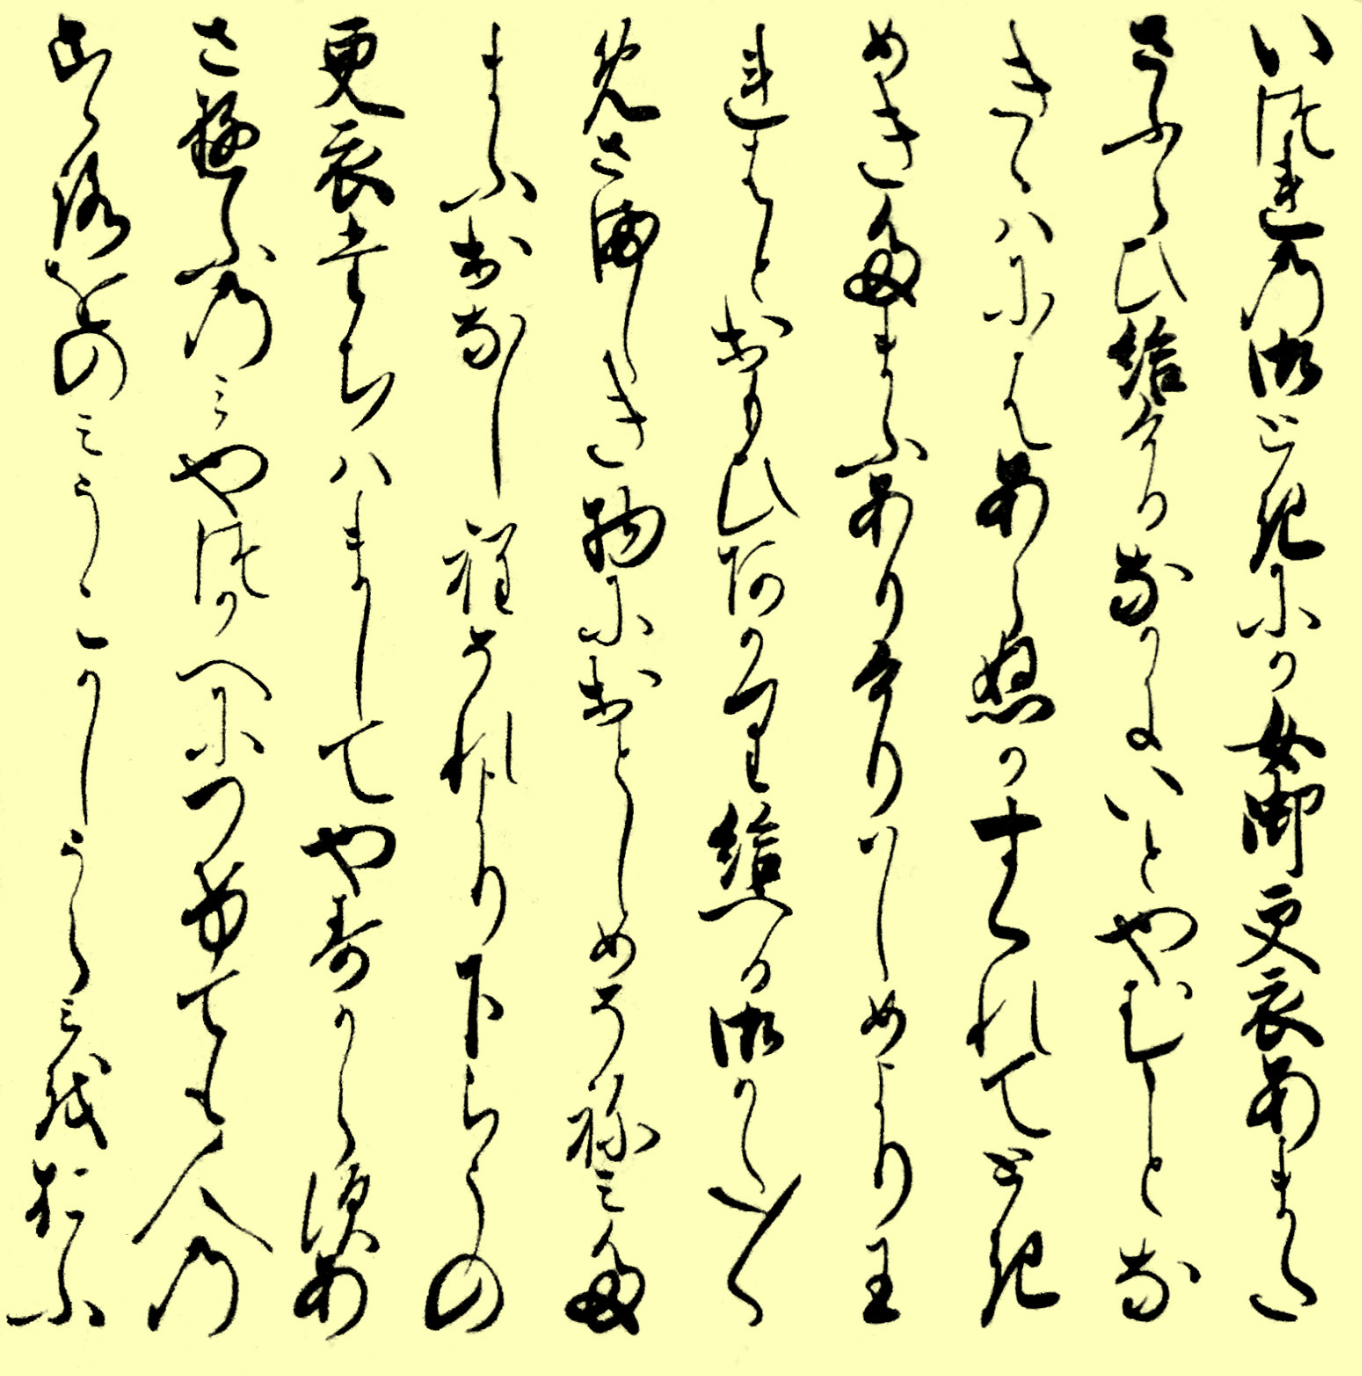
\includegraphics[width=0.55\textwidth]{graphics/genji1}\\
  {\tiny (\citealt{Rickmeyer1991}; 源氏物語:きりつぼ, ca. 1000 u.\,Zr., Manuskript (青表紙証本) ca.\ 1200 u.\,Zr.}
\end{frame}

\begin{frame}
  {Scriptio continua: Genji no Monogatari}
  \centering
  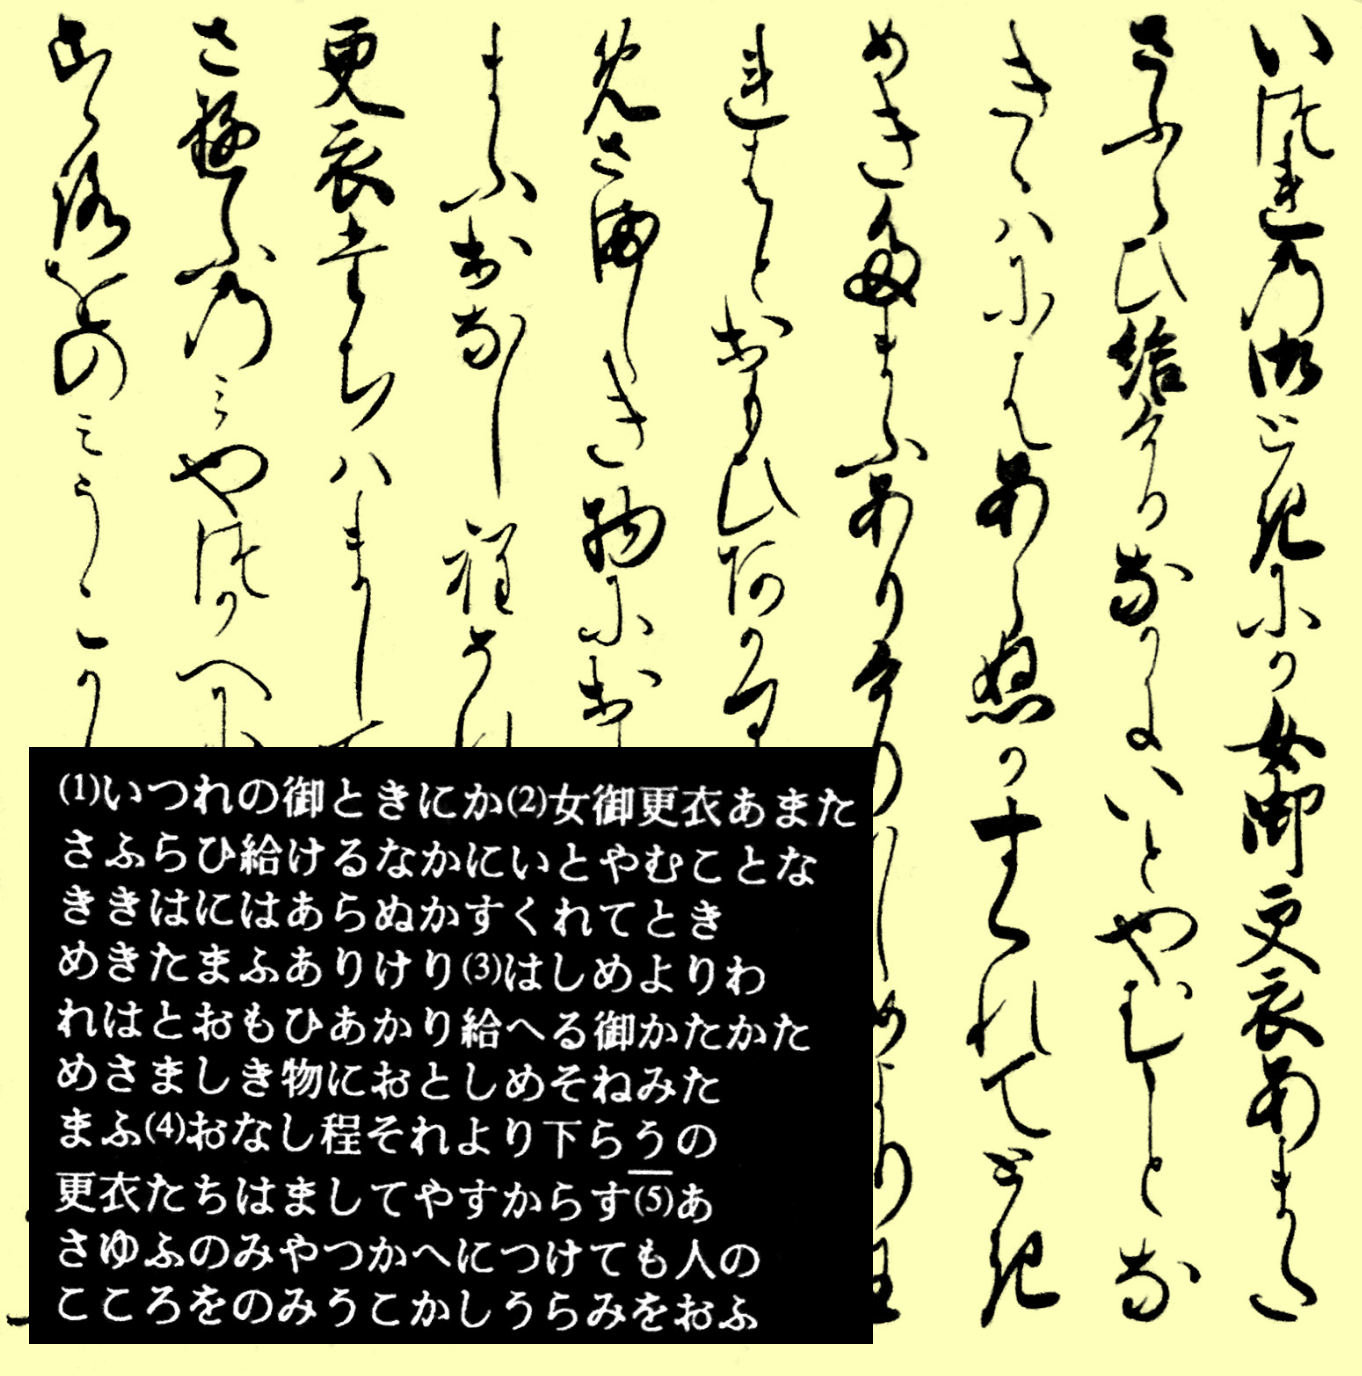
\includegraphics[width=0.55\textwidth]{graphics/genji3}\\
  {\tiny (\citealt{Rickmeyer1991}; 源氏物語:きりつぼ, ca. 1000 u.\,Zr., Manuskript (青表紙証本) ca.\ 1200 u.\,Zr.}
\end{frame}

\begin{frame}
  {Wie selbstverständlich ist unsere Schreibung?}
  \pause
  \centering
  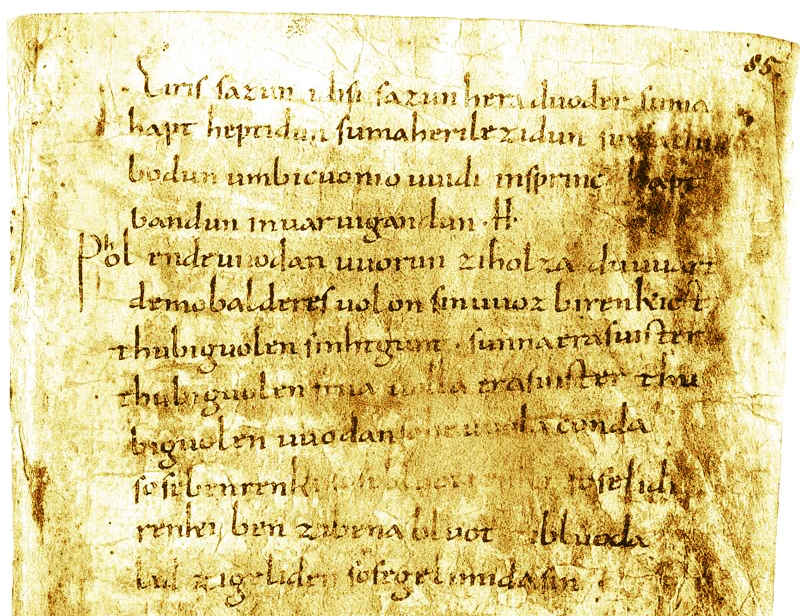
\includegraphics[width=0.8\textwidth]{graphics/merseburg}\\[0.5\baselineskip]
  {\tiny 1.~und 2.~Merseburger Zauberspruch, 9.~Jh.\ u.\,Zr., Cod.\ 136, Folio 85r, Domstiftsbibliothek Merseburg (Wikimedia)\\[-1\baselineskip]
    Hintergründe und generelle Einführung in historische Graphematik in \citet{Elmentaler2018}.}
\end{frame}

\begin{frame}
  {Spatien}
  \pause
  \begin{itemize}[<+->]
    \item im Ahd.\ häufig Reste von Scriptio continua
    \item syntaktische Wörter nicht immer getrennt
    \item \alert{Spatienschreibung}: Trennung syntaktischer Wörter
  \end{itemize}
  \pause
  \Halbzeile
  \begin{exe}
    \ex
    \begin{xlist}
      \ex[*]{Vanessa \rot{istgeritten}.}
      \pause
      \ex[*]{Vanessa reitet \rot{indenwald}.}
    \end{xlist}
    \pause
    \Halbzeile
    \ex
    \begin{xlist}
      \ex[*]{Vanessa hat \rot{Gelegen heit}, die \rot{Schreib ung} von Wörtern und Sätzen \rot{gründ lich} zu \rot{unter suchen}.}
      \pause
      \ex[*]{Oma \rot{koch t} der \rot{ausgekühlt en} Vanessa \rot{ein en heiß en} Tee.}
    \end{xlist}
  \end{exe}
  \pause
  \begin{itemize}[<+->]
    \item Eislaufen, Bergsteigen, Mutmachen, Teetrinken (?)
    \item weichklopfen, schlechtreden (?)
    \item nichtöffentlich, nichtprivat (?)
    \item zulasten (?)
  \end{itemize}
\end{frame}

\section[PUMS vs.\ PAMS]{Positionsunabhängige Majuskelschreibung}

\begin{frame}
  {Majuskelschreibungen}
  \pause
  \begin{itemize}[<+->]
    \item \alert{positionsabhängig}: Satzanfang (Syntax)
      \Halbzeile
    \item \alert{positionsunabhängig}: Substantive (Morphologie\slash Lexik)
    \item Positionsunabhängige Majuskelschreibung (PUMS)
      \Halbzeile
    \item Bredel: "`NP-Kopf-Großschreibung"' (= positions\rot{abhängig}, PAMS)
      \begin{itemize}[<+->]
        \item nein, weil auch in Listen, Überschriften usw.
        \item außerdem: dann Annahme SubstP als verschieden von PronP!\\
          \grau{Oder werden Pronomina als NP-Köpfe großgeschrieben?}
        \item jede Rettungsargumentation des PAMS-Ansatzes wird zirkulär 
        \item \ldots oder \alert{motiviert} die PUMS statt sie zu beschreiben
        \item \grau{Siehe Schäfer \& Sayatz (in Vorb.).}
      \end{itemize}
  \end{itemize}
\end{frame}


\begin{frame}
  {Propblemfälle für PUMS}
  \pause
  \begin{exe}
    \ex
    \begin{xlist}
      \ex{An der Nacht auf dem Land schätze ich vor allem \alert{das Dunkle}.}
      \pause
      \ex{Alle Pferde müssen geputzt werden. Vanessa putzt \alert{das schwarze}.}
      \pause
      \ex{Vanessa trägt in der Oper \alert{das Schwarze}.}
    \end{xlist}
    \Viertelzeile
    \pause
    \ex
    \begin{xlist}
      \ex[ ]{im \alert{übrigen}}
      \pause
      \ex[*]{im literarischen \rot{Übrigen}}
      \pause
      \ex[*]{Im \rot{Übrigen}\slash In dem \rot{Übrigen}, von dem wir gestern schon gesprochen haben, ist dieses Buch langweilig.}
    \end{xlist}
    \pause
    \Viertelzeile
    \ex
    \begin{xlist}
      \ex[*]{Edgar gab dem Kunden fachmännisches Recht.}
      \pause
      \ex[*]{Edgar setzte den Cadillac in einwandfreien Stand.}
    \end{xlist}
  \end{exe}
  \pause
  \begin{itemize}[<+->]
    \item Konversion
    \item Ellipse
    \item Ellipse plus Lexikalisierung
      \Halbzeile
    \item mögliches Testkriterium bei \alert{Univerbierung}: Modifikation
  \end{itemize}
\end{frame}

\section[Konstanz]{Konstantschreibung}

\begin{frame}
  {Die Entwicklung von Schreibprinzipien}
  \pause
  \centering
  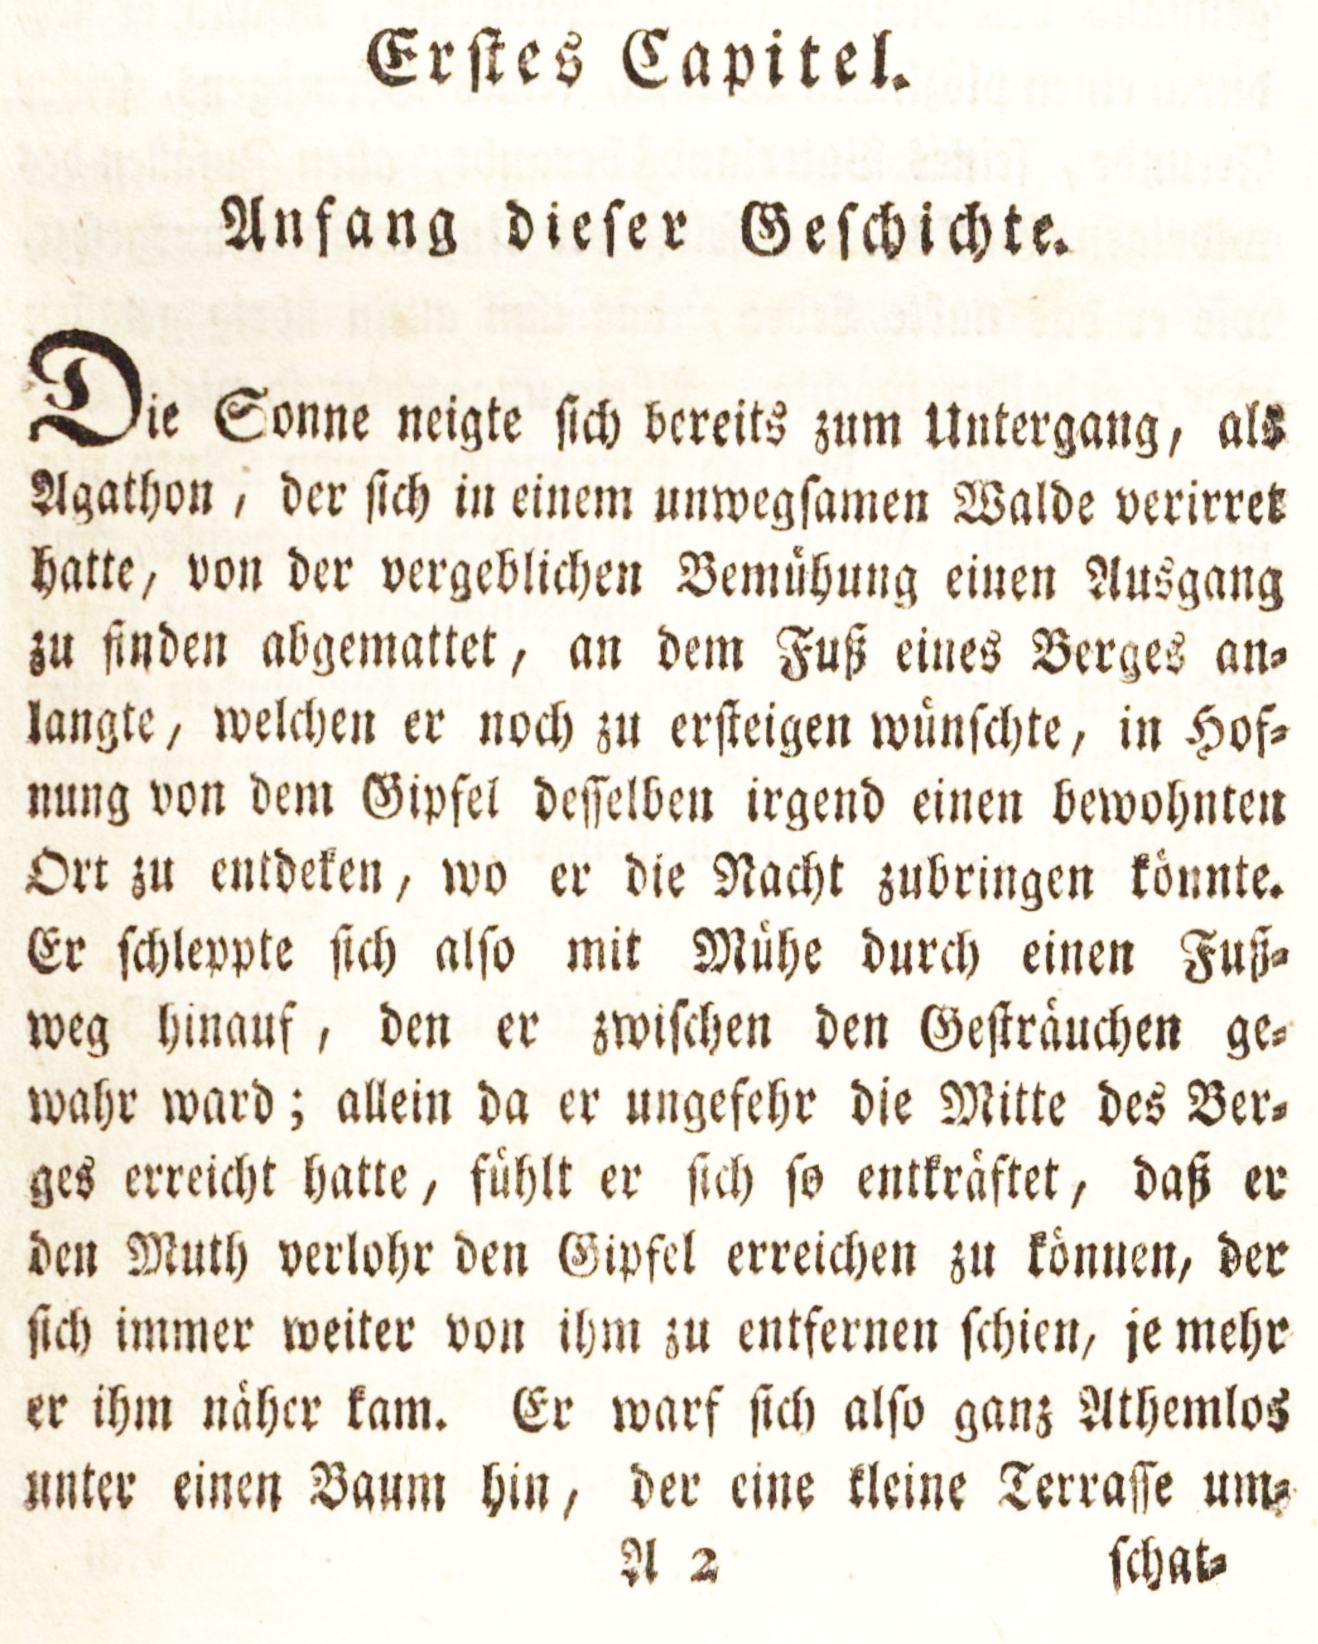
\includegraphics[width=0.45\textwidth]{graphics/agathon1e}\\[0.5\baselineskip]
  {\tiny Wieland, Christoph Martin: Geschichte des Agathon. Bd.\ 1. Frankfurt (Main) u.\,a., 1766. In: Deutsches Textarchiv\\[-1\baselineskip]
    \url{http://www.deutschestextarchiv.de/wieland_agathon01_1766>}}
\end{frame}

\begin{frame}
  {Die Entwicklung von Schreibprinzipien}
  \centering
  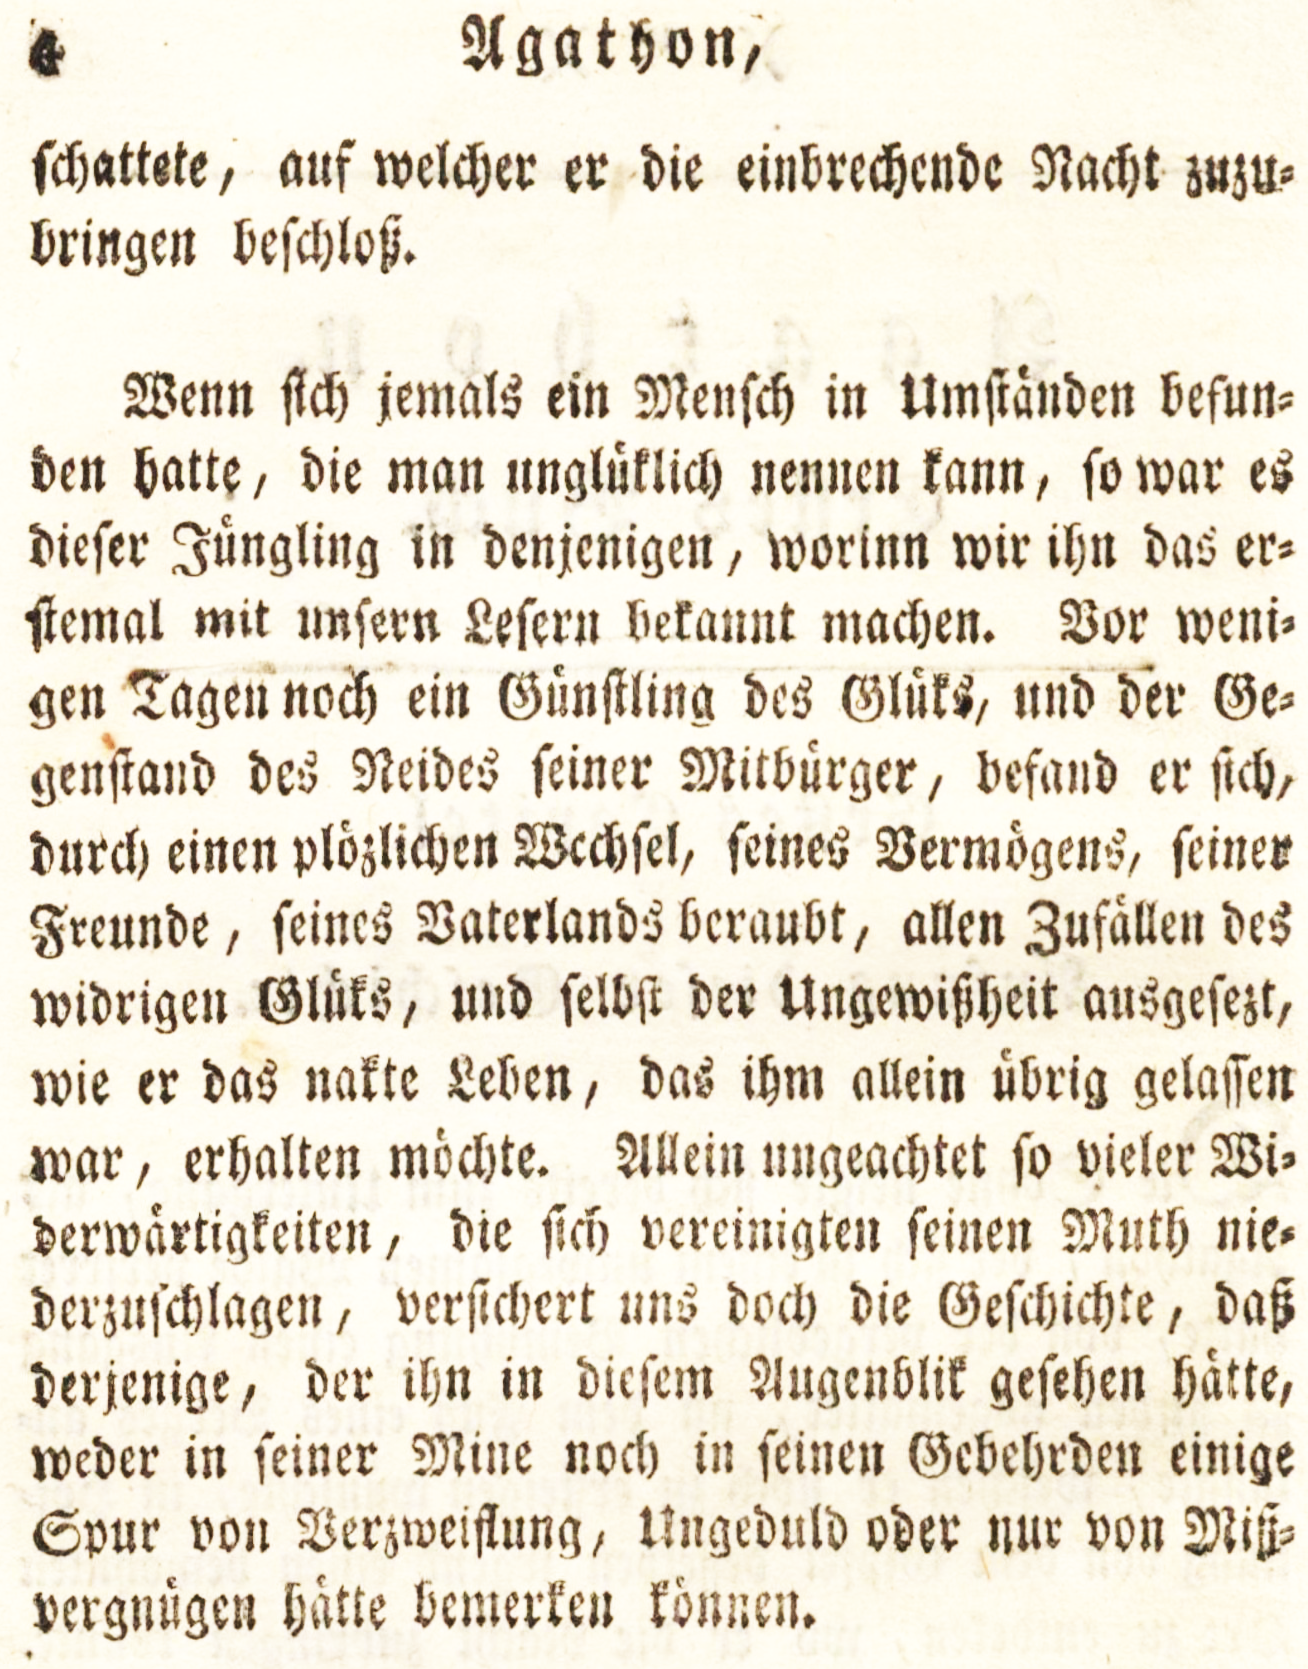
\includegraphics[width=0.45\textwidth]{graphics/agathon2e}\\[0.5\baselineskip]
  {\tiny Wieland, Christoph Martin: Geschichte des Agathon. Bd.\ 1. Frankfurt (Main) u.\,a., 1766. In: Deutsches Textarchiv\\[-1\baselineskip]
    \url{http://www.deutschestextarchiv.de/wieland_agathon01_1766>}}
\end{frame}

\begin{frame}
  {Zur Erinnerung: unerklärte Doppelkonsonanten}
  \pause
  \centering
  \resizebox{0.85\textwidth}{!}{
    \begin{tabular}{lllllllll}
      \toprule
      & & & \textbf{ɪ} & \textbf{ʊ} & \multicolumn{2}{l}{\LocStrutGrph\textbf{ɛ̆}} & \textbf{ɔ} & \textbf{ă} \\
      \midrule

      \multirow{4}{*}{\rotatebox{90}{\textbf{ungespannt}}}

      & \multirow{2}{*}{\rotatebox{90}{\textbf{offen}}}
      & \textbf{einsilb.}  & \textit{\Nono}  & \textit{\Nono}           & \multicolumn{2}{l}{\LocStrutGrph\textit{\Nono}}         & \textit{\Nono}        & \textit{\Nono}           \\
      && \textbf{zweisilb.}  & \textit{Li.\alert{pp}e} & \textit{Fu.\alert{tt}er}         & \multicolumn{2}{l}{\LocStrutGrph\textit{We.\alert{ck}e}}        & \textit{o.\alert{ff}en}       & \textit{wa.\alert{ck}er}         \\
        & \multirow{2}{*}{\rotatebox{90}{\textbf{gesch.}}}
        & \textbf{einsilb.}  & \textit{Ki\rot{nn}}   & \textit{Schu\rot{tt}}    & \multicolumn{2}{l}{\LocStrutGrph\textit{Be\rot{tt}}}           & \textit{Ro\rot{ck}}         & \textit{Wa\rot{tt}}            \\
        && \textbf{zweisilb.}  & \textit{Rin.de} & \textit{Wun.der}        & \multicolumn{2}{l}{\LocStrutGrph\textit{Wen.de}}        & \textit{pol.ter}      & \textit{Tan.te}          \\

      \midrule

      \multirow{4}{*}{\rotatebox{90}{\textbf{gespannt}}}

      & \multirow{2}{*}{\rotatebox{90}{\textbf{offen}}}
        & \textbf{einsilb.}  & \textit{Knie}   & \textit{Schuh}       & \textit{Schnee, Reh}  & \textit{zäh}          & \textit{roh}          & (\textit{da})            \\
      && \textbf{zweisilb.}  & \textit{Bie.ne} & \textit{Kuh.le, Schu.le} & \textit{we.nig}       & \textit{Äh.re, rä.kel} & \textit{oh.ne, O.fen} & \textit{Fah.ne, Spa.ten} \\

      & \multirow{2}{*}{\rotatebox{90}{\textbf{gesch.}}}
        & \textbf{einsilb.}  & \textit{lieb}  & \textit{Ruhm, Glut}      & \textit{Weg}          & \textit{spät}           & \textit{rot}          & \textit{Tat}             \\
      && \textbf{zweisilb.}  & (\textit{lieb.lich}) & (\textit{lug.te})   & (\textit{red.lich})   & (\textit{wähl.te})     & (\textit{brot.los})   & (\textit{rat.los})       \\

      \midrule
      & & & \textbf{i} & \textbf{u} & \textbf{e} & \textbf{ε} & \textbf{o} & \textbf{a} \\

      \bottomrule
    \end{tabular}
  }\\
  \pause
  \Viertelzeile
  \raggedright
  \begin{itemize}[<+->]
    \item Warum \textit{Kinn}, \textit{Schutt}, \textit{Bett}, \textit{Rock}, \textit{Wattes}?
    \item \alert{nicht unterlassbare Gelenkschreibungen}
      \begin{itemize}[<+->]
        \item \textit{die Ki\alert{nn}e}
        \item \textit{des Schu\alert{tt}es}
        \item \textit{die Be\alert{tt}en}
        \item \textit{die Rö\alert{ck}e}
      \end{itemize}
    \item \alert{Die Schreibungen eines Stamms einander angleichen!} Sonst:
      \begin{itemize}[<+->]
        \item \textit{*Kin --- Kinne}
        \item \textit{Schut --- Schutt}
        \item \textit{Bet --- Betten}
        \item \textit{Rok --- Röcke}
      \end{itemize}
  \end{itemize}
\end{frame}

\begin{frame}
  {Andere Konstantschreibungen}
  \pause
  \begin{itemize}[<+->]
    \item andere Wortklassen
      \begin{itemize}[<+->]
        \item \textit{*plat --- pla\rot{tt} --- pla\alert{tt}er}
        \item \textit{*as --- a\rot{ß} --- a\alert{ß}en}
        \item aber: \textit{las --- lasen}
        \item \textit{*schlizte --- schli\rot{tz}te --- schli\alert{tz}en}
      \end{itemize}
      \Halbzeile
    \item andere Phänomene (nicht Silbengelenk oder \textit{ß})
      \begin{itemize}[<+->]
        \item \textit{*gest --- ge\rot{h}st --- ge\alert{h}en}
        \item \textit{*siest --- sie\rot{h}st --- se\alert{h}en}
        \item \textit{*Reume --- R\rot{äu}me --- R\alert{au}m}
        \item \textit{*leuft --- l\rot{äu}ft --- l\alert{au}fen}
      \end{itemize}
  \end{itemize}
\end{frame}

\section{Schreibprinzipien}

\begin{frame}
  {Zusammenfassung der besprochenen Schreibprinzipien I}
  \pause
  Korrespondenzen zur Phonologie\\
  \Zeile
  \pause
  \begin{itemize}[<+->]
    \item \alert{phonologisches Schreibprinzip}
      \begin{itemize}[<+->]
        \item Konsonantenzeichen (inkl.\ Di- und Trigraphen)\\
          entsprechen 1:1 zugrundeliegenden Segmenten.
        \item Paare von zugrundeliegendem gespanntem und ungespanntem Vokal\\
          entsprechen jeweils nur einem Vokalzeichen 
      \end{itemize}
     \Zeile 
    \item \alert{Prinzip der Silbengelenkschreibung}
      \begin{itemize}[<+->]
        \item Silbengelenke werden durch Konsonantendopplung markiert.
        \item Für Di- und Trigraphen gilt dies nicht.
      \end{itemize}
  \end{itemize}
\end{frame}

\begin{frame}
  {Zusammenfassung der besprochenen Schreibprinzipien II}
  Korrespondenzen zur Morphosyntax\\
  \Zeile
  \pause
  \begin{itemize}[<+->]
    \item \alert{Prinzip der Konstantschreibung}
      \begin{itemize}[<+->]
        \item Die Formen eines lexikalischen Wortes werden so ähnlich geschrieben,\\
          wie es angesichts der anderen Prinzipien möglich ist.
      \end{itemize}
      \Zeile
    \item \alert{Prinzip der Spatienschreibung}
      \begin{itemize}[<+->]
        \item Syntaktische Wörter werden durch Spatium getrennt.
        \item \grau{Zweifelsfälle dabei sind morphosyntaktisch, nicht graphematisch.}
      \end{itemize}
      \Zeile
    \item \alert{Prinzip der positionsunabhängige Majuskelschreibung}
      \begin{itemize}[<+->]
        \item Substantive werden positionsunabhängig\\
          mit einleitender Majuskel geschrieben.
      \end{itemize}
  \end{itemize}
\end{frame}

\begin{frame}
  {Das wars!}
  \pause
  \begin{itemize}[<+->]
    \item Das war der Stoff der VL dieses Semesters.
    \item \alert{Vielen Dank fürs Zuhören und Fragenstellen!}
    \item Trotz der Arbeitsbelastung hat mir diese die Lehrveranstaltung\\
      den meisten Spaß in meiner gesamten Zeit als Dozent*in gemacht.
      \Zeile
    \item Jetzt kommt noch zweimal "`ernste Worte"'.
    \item Die Folien enthalten viel Text (ganze Sätze!), weil Sie das\\
      sonst nirgendwo nachlesen können.
      \Halbzeile
    \item Dann endlich die Klausurbesprechung!
  \end{itemize}
\end{frame}

\section{Alles falsch?}

\begin{frame}
  {Nochmal zur Grammatik in der Schule}
  \pause
  Wie ich höre\ldots
  \pause
  \begin{itemize}[<+->]
    \item \rot{Frustration} darüber, was alles \textit{falsch} sein soll
    \item insbesondere (angeblich) in Schulbüchern
      \Halbzeile
    \item außerdem: \alert{Es funktioniert doch!}
  \end{itemize}
\end{frame}
  
  
  
\begin{frame}
  {Deutschunterricht}
  \pause
  \alert{Worum geht es in der Schule beim Deutschunterricht nochmal?}\\
  \Halbzeile
  \pause
  \begin{itemize}[<+->]
    \item Erwerb von Schrift (= Zeichen) und Schreibung (= Prinzipien)
    \item Erwerb der \alert{Schriftsprache} (= \alert{völlig neue Grammatik})
    \item Erwerb der \alert{überregionalen Standardsprache} (= neue Grammatik)
    \item Erwerb der \alert{Bildungssprache} (basiert stark auf Schriftsprache)
      \begin{itemize}[<+->]
        \item komplexe Sachverhalte
        \item argumentative Strukturen
        \item Registersensitivität
        \item Variantenbewusstsein, \ldots
        \item \alert{und die zugehörigen sprachlichen Formen}
      \end{itemize}
      \Halbzeile
    \item Ist Deutsch eigentlich ein ungewöhnliches Schulfach?
  \end{itemize}
\end{frame}

\begin{frame}
  {Möglichkeit A: das Wissen an sich}
  \pause
  \begin{itemize}[<+->]
    \item \alert{Schulfächer lehren selbstbewusst ihre \alert{Inhalte}:}
      \begin{itemize}[<+->]
        \item Biologie: Ranviersche Schnürringe, Natrium-Kalium-Pumpe, \ldots
        \item Geschichte: Schlacht von Worringen, Hanse, Völkerwanderung, \ldots
        \item Erdkunde: Löss-Böden, Schwemmland, Kontinentaldrift, \ldots
        \item Physik: idealisierte Wagen auf idealisierten schiefen Ebenen,\\
          Gravitationsgesetze, Ohmsches Gesetz, \ldots
        \item Chemie: Wasserstoffbrückenbindungen, Schalenmodell, Veresterung, \ldots
        \item Mathematik: Ableiten und Integrieren, Vektor- und Matrizenrechnung, \ldots
      \end{itemize}
      \Viertelzeile
    \item Das ist Wissen darum, wie die Welt funktioniert.
    \item Es gibt ein Verständnis für die westlich-wissenschaftliche Weltsicht.
    \item \rot{Was davon erwarten Sie, im Leben praktisch zu brauchen?}
  \end{itemize}
\end{frame}

\begin{frame}
  {Und das Schulfach Deutsch?}
  \pause
    \begin{itemize}[<+->]
      \item Erwerbsaufgaben (\rot{keine} Wissensvermittlung): Das muss ja sein. 
      \item Literatur: recht selbstbewusst (\zB wichtige Werke der dt.\ Literatur)
        \Halbzeile
      \item Wissen darum, wie Sprache funktioniert: \rot{Oh Gott! Nein! Das hat ja\\
        gar keinen praktischen Nutzen (jenseits der Erwerbsaufgaben)!}
    \end{itemize}
\end{frame}

\begin{frame}
  {Das Problem mit Wissen an sich: die Genauigkeit!}
  \pause
  \begin{itemize}[<+->]
    \item Angenommen, es würden grammatische\slash linguistische Inhalte\\
      als Fachwissen an Schulen gelehrt\ldots
    \item \alert{Dann müsste es aber sachlich korrekt sein bzw.\\
      dem Forschungsstand entsprechen!}
      \Halbzeile
    \item \rot{Das, was in Grammatik unterrichtet wird, entspricht\\
      auf jeden Fall nicht dem Forschungsstand.}
      \Zeile
    \item Es lassen sich de facto seit 50 Jahren kaum Änderungen\\
      am Schulstoff politisch durchsetzen.
    \item Die Linguistik hat in den Siebzigern ihren Teil dazu beigetragen,\\
      dass es große Skepsis ihr gegenüber (als Fachdisziplin) gibt.
    \item Man wollte Chomskys "`Generative Transformationsgrammatik"'\\
      an die Schulen bringen.
    \item \raisebox{-.2\height}{
\includegraphics[width=1.25em]{graphics/emoji_mourning}}
  \end{itemize}
\end{frame}

\begin{frame}
  {Möglichkeit B: vor allem die Erwerbsaufgaben}
  \pause
  \begin{itemize}[<+->]
    \item Das entspricht dem Ist-Zustand.
    \item Meinethalben kann das so bleiben.
      \Halbzeile
    \item Was ist dann wichtig?
      \begin{itemize}[<+->]
        \item \alert{Sprachbetrachtung} (= Reflexion über Form und Funktion)
        \item unmöglich exhaustiv unterrichtbar, also \alert{Methodenvermittlung}
        \item für deklarativen Kern: \alert{widerspruchsfrei, dem Phänomen angemessen}
      \end{itemize}
  \end{itemize}
\end{frame}


\begin{frame}
  {Anforderungen bei Möglichkeit B}
  \pause
    \begin{itemize}[<+->]
      \item \alert{Form und Funktion der eigenen Sprache verstehen}
      \item selber in der Lage sein, \alert{Generalisierungen zu erarbeiten}
      \item zum Phänomen \alert{das passende Material zusammenstellen}
      \item \alert{Operationalisierungen} erarbeiten und Schüler*innen anbieten
        \Halbzeile
      \item \rot{Erkennen und Einstufen von Erwerbsproblemen}
        \Halbzeile
      \item \rot{fair und begründet bewerten}
        \Halbzeile
      \item \rot{Die Didaktisierung kann nicht darin bestehen, den Schüler*innen\\
        Material und Methoden anzubieten, aus denen die entsprechenden\\
      Kompetenzen prinzipiell nicht erwerbbar sind.}
      \Halbzeile
    \item Beispiel: die \textit{Wie}-Wörter
      \begin{itemize}[<+->]
        \item \textit{der rote Trecker}
        \item \textit{Wie ist der Trecker?} --- \alert{(\textit{Der Trecker ist}) \textit{rot.}}
        \item \grau{Die Antwort ist immer ein Kopulsatz.}
      \end{itemize}
  \end{itemize}
\end{frame}

\begin{frame}
  {Ein Beispiel: Adjektive als Wie-Wörter}
  \begin{itemize}[<+->]
    \item OK für bestimmte \alert{qualitative Adjektive}
      \Halbzeile
    \item viele Adjektivklassen sind aber keine Wie-Wörter:
      \begin{itemize}[<+->]
        \item \rot{temporal}: der \rot{gestrige} Vorfall
        \item \rot{quantifizierend} (relativ, Zählsubstantiv): \textit{die \rot{zahlreichen} Äpfel}
        \item \rot{quantifizierend} (relativ, Stoffsubstantiv): \textit{\rot{reichlich} Apfelmus}
        \item \rot{quantifizierend} (absolut): \textit{die \rot{drei} Bienen}
        \item \rot{intensional}: \textit{der \rot{ehemalige} Präsident}\slash\textit{die \rot{fiktive} Gestalt}
        \item \rot{phorisch}: \textit{die \rot{obigen}}/\textit{\rot{weiteren}}/\textit{\rot{anderen} Ausführungen}
        \item \rot{qualitativ-relativ} (sortensensitiv): \textit{eine \rot{schnelle} Schnecke}
      \end{itemize}
      \Halbzeile
    \item Fällt Ihnen was auf?
      \begin{itemize}[<+->]
        \item Das sind im Wesentlichen die, die nicht prädikativ verwendbar sind.
        \item Ach, basiert der Test also vielleicht einfach darauf?
        \item Aber viele Adjektive sind doch gar nicht prädikativ verwendbar.
          \Halbzeile
%        \item[ ] \raisebox{-0.5\height}{
\includegraphics[width=3em]{graphics/doh}}
        \item[ ] \raisebox{-0.5\height}{
\includegraphics[height=4em]{graphics/doh}}
      \end{itemize}
  \end{itemize}
\end{frame}

\begin{frame}
  {Inhaltliche Stolperfallen}
  \pause
  \begin{itemize}[<+->]
    \item linguistisch eine klare Angelegenheit:
      \begin{itemize}[<+->]
        \item \rot{Die Kategorie \textit{Adjektiv} kann man nicht über "`wie"' erfragen!}
        \item im Prinzip nur die Subklasse der prädikativ verwendbaren Adjektive
      \end{itemize}
     \Halbzeile
    \item inhaltliche Gefahr
      \begin{itemize}[<+->]
        \item Wenn Sie Kinder dressieren, \rot{alle} Klassen mit "`wie"' zu erfragen\ldots
        \item \ldots dann \rot{zerstören Sie die wahrscheinlich bereits existierende semantische Intuition}, die das Kind hat.
          \Halbzeile
        \item \rot{Totalschaden in Vermittlung von Bildungssprache\slash Sprachbetrachtung}
      \end{itemize}
  \end{itemize}
\end{frame}

\begin{frame}
  {Didaktische Stolperfallen}
  \pause
  \begin{itemize}[<+->]
    \item didaktische Gefahr
      \begin{itemize}[<+->]
        \item "`Die Kinder können es doch gut mit der Wie-Frage!"' (s. nächste Folie)
      \end{itemize}
      \Halbzeile
    \item Fragen Sie immer:
      \Halbzeile
      \begin{itemize}[<+->]
        \item Ist das, was ich unterrichte (vor-)wissenschaftliches Wissen an sich \alert{und gibt präzise linguistische Generalisierungen wieder?} --- \gruen{OK!}
          \Halbzeile
        \item Oder trägt es zur Sprach(betrachtungs)kompetenz de*r Schüler*innen bei, indem sie durch die Übung \alert{Kompetenzen} erwerben, die zur \alert{besseren Beherrschung sprachlicher Mittel} (i.\,w.\,S.) führen? --- \gruen{OK!}
          \Halbzeile
        \item Keins von beidem? --- \rot{Nicht OK!} Dann lassen Sie es lieber.
      \end{itemize}
  \end{itemize}
\end{frame}

\begin{frame}
  {Eine Aufgabe zu Adjektiven I}
  \pause
  Warum können die Kinder das so gut mit der Wie-Frage?\\
  \Halbzeile
  \pause
  \centering
  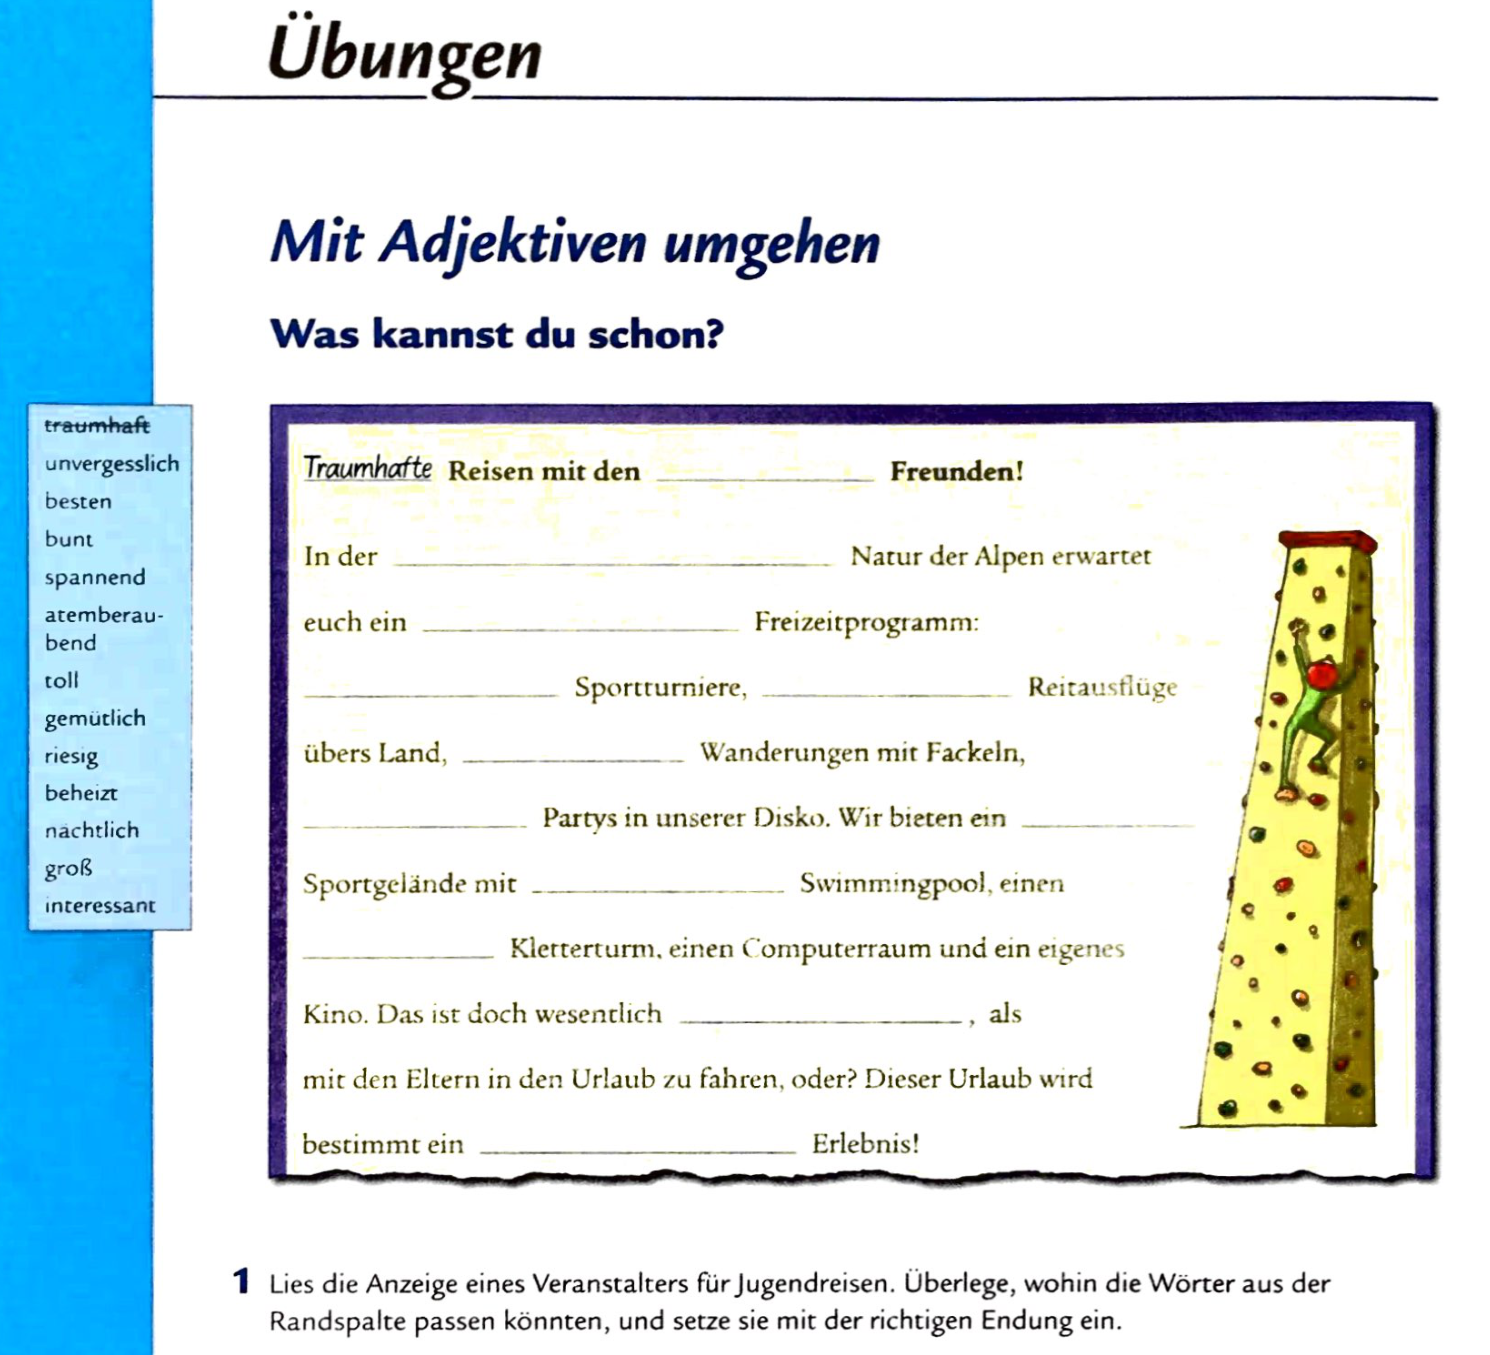
\includegraphics[width=0.65\textwidth]{graphics/adjektive1}
%  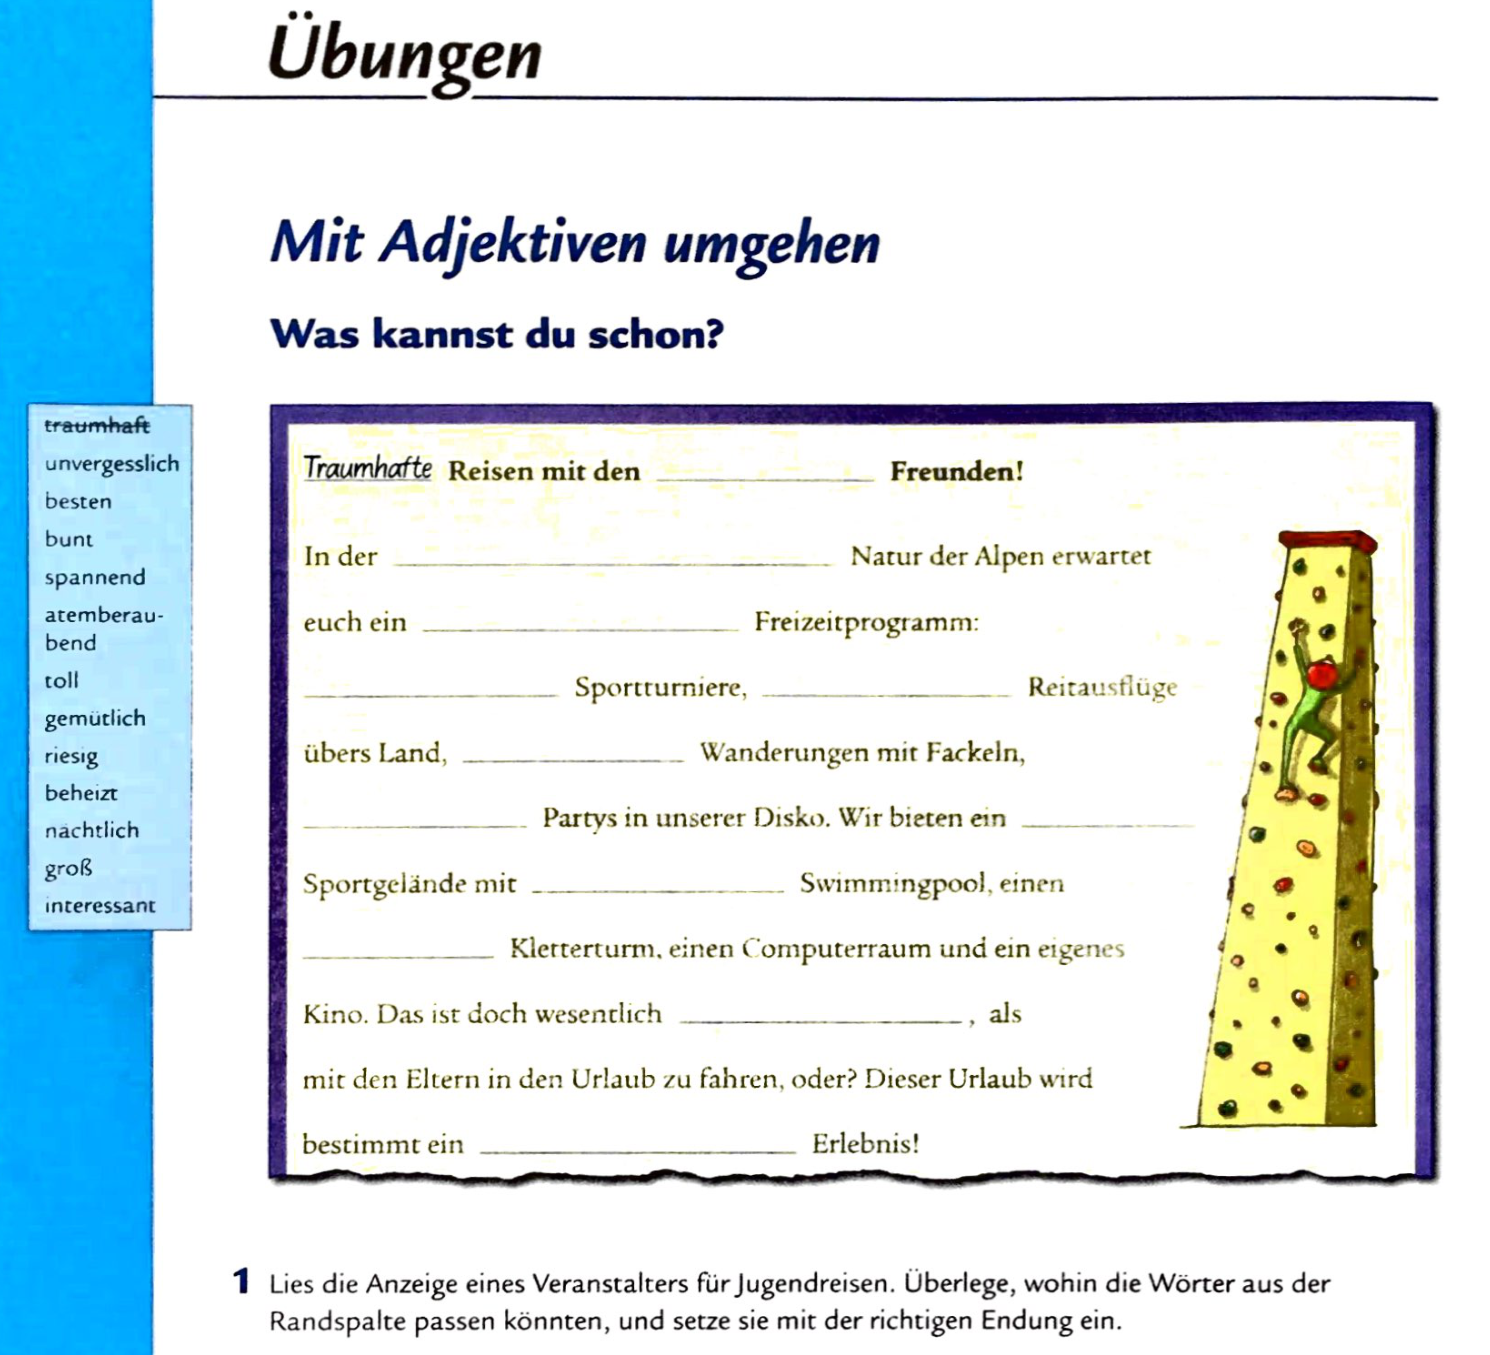
\includegraphics[width=0.65\textwidth]{graphics/adjektive1}
\end{frame}

\begin{frame}
  {Eine Aufgabe zu Adjektiven II}
  Gut! Bezug zur Funktion sprachlicher Mittel. Aber\ldots\\
  \Zeile
  \pause
  \centering
  
\includegraphics[width=0.7\textwidth]{graphics/adjektive2}
%  
\includegraphics[width=0.7\textwidth]{graphics/adjektive2}
\end{frame}

\section{Meine Meinung zu sprachlicher Toleranz}

\begin{frame}
  {Das tut ja weh!}
  \pause
  Angeblich wurden folgende Sätze als schmerzhaft (sic!) falsch empfunden.
  \pause
  \Viertelzeile
  \begin{exe}
    \ex \rot{Es friert mich}.
    \pause
    \ex Die Mechanikerin \rot{bekommt} von der Auszubildenden \rot{geholfen}.
    \pause
    \ex Die Erklärung \rot{macht Sinn}.
    \pause
    \ex \rot{Gebe} deiner Schwester jetzt das Buch.
  \end{exe}
  \pause
  \begin{itemize}[<+->]
    \item Das ist die bildungssprachliche Verwendung von \textit{frieren}! (Duden 1)
    \item \alert{Rezipientenpassiv ist auch geschrieben Standard} (Duden 4, §807–810).
      \begin{itemize}[<+->]
        \item Meist "`akzeptabler"' mit Akkusativ:\\
          \textit{Elena bekam von der Trainerin die Sprungtechnik erklärt.}
        \item partiell \alert{regionale Variation} (\textit{erhalten}, \textit{bekommen}, \textit{kriegen})
      \end{itemize}
    \item \textit{Sinn machen} kommt nicht aus dem Englischen und ist uralt.
    \item \alert{Der normalisierte Imperativ der vierstufigen Verben ist regional üblich},\\
      wird aber in der Tat im Standard nicht empfohlen (Duden 4, §609)
    \item \rot{Auf jeden Fall geht es um die alltägliche Sprache Ihrer Mitmenschen!}
  \end{itemize}
\end{frame}

\begin{frame}
  {Standard und andere Varietäten}
  \pause
  \begin{itemize}[<+->]
    \item Standard ist ein \alert{Kompromiss}, ein \alert{Versuch} den kleinsten gemeinsamen \alert{überregionalen und nicht soziolektal geprägten sprachlichen} Nenner zu beschreiben.
    \item hat nichts mit \rot{alt} oder \rot{ursprünglich} zu tun, wird \alert{ständig angepasst}
      \Halbzeile
    \item \alert{Lehrer*innen sind für die Vermittlung des Standards zuständig.}
    \item \rot{Aber was erlaubt es irgendwem, die Sprache anderer\\
      als schmerzhaft oder ekelhaft zu bezeichnen?}
  \end{itemize}
\end{frame}

\begin{frame}
  {Die Provokationsfolie}
  \pause
  \begin{itemize}[<+->]
    \item Wie finden Sie das?
      \Halbzeile
      \begin{itemize}[<+->]
        \item "`Häng dir was vors Gesicht. Deine Augen sind ekelhaft."'
          \Viertelzeile
        \item Bei deiner Figur sieht das Hemd echt widerlich aus.
          \Viertelzeile
        \item "`Die Schwulen sollen doch woanders hingehen. Ich muss kotzen."'
          \Viertelzeile
        \item Sag nicht nochmal "`Sie bekommt geholfen."' Das tut ja weh.
          \Viertelzeile
        \item Wir verkaufen nur an Weiße\slash Arier\slash\ldots.
          \Viertelzeile
        \item "`Roberto Blanco war immer ein wunderbarer Neger."'
          \Viertelzeile
        \item Der sagt "`isch"' statt "`ich"'. Wir stellen wohl lieber jemanden ein,\\
          der richtiges Deutsch kann.
      \end{itemize}
      \Zeile
    \item Unterschied: \rot{Grad der Explizitheit\slash Implizitheit der Diskriminierung}
  \end{itemize}
\end{frame}


\begin{frame}
  {Diskriminierung, offen oder versteckt?}
  \pause
  \begin{itemize}[<+->]
    \item Implizite Diskriminierung (\zB gegenüber Migrant*innen,\\
      LGBTQ-Personen) ist unser Hauptproblem "`in Diskriminierung"'.
    \item \rot{Erfahrungsgemäß kann implizite Diskriminierung\\
      jederzeit explizit werden.}
      \Halbzeile
    \item Implizit heißt eben auch \alert{unbewusst}. Das ist schnell passiert.
      \Halbzeile
    \item Ich nehme mich überhaupt nicht aus und sehe mich als Lernende*.
    \Halbzeile
  \end{itemize}
\end{frame}

\begin{frame}
  {Standard\slash Dialekt\slash Soziolekt in der Schule}
  \pause
  \begin{itemize}[<+->]
    \item \rot{auf keinen Fall sprachliche Diskriminierung}
    \item im Gegenteil: \alert{Dia- und Soziolekte erhalten}
    \item Standard \alert{bewusst als neue zusätzliche Varietät} unterrichten,\\
      die genau definierte\alert{Anwendungskontexte} hat\\
      (= Variantenbewusstsein)
      \Halbzeile
    \item nicht unselektiv\slash pauschal "`richtig"' gegen "`falsch"' stellen
    \item vor allem \rot{niemals nach "`Geschmacksurteilen"' bewerten},\\
      denn \rot{Lehrer*innen korrigieren oft inkonsistent} und\\
      streichen viel mehr als falsch an, als wirklich normativ falsch ist\\
      (\citealt[4--7]{Eisenberg2004}, \citealt[319--324]{Haecker2009})
      \Halbzeile
    \item \alert{Wenn Sie es nicht genau wissen, schauen Sie es nach!}
    \item \ldots oder diskutieren Sie das Phänomen im Rahmen des Systems.
  \end{itemize}
\end{frame}


\section{Vorschau}

\begin{frame}
  {Was heißt Klausurvorbereitung?}
  \pause
  \begin{itemize}[<+->]
    \item inhaltliche Fragen?
    \item Fragen zur Probeklausur?
    \item ansonsten meine vorbereiteten Übungen
  \end{itemize}
  \pause
  \Halbzeile
  \begin{center}
    Bitte lesen Sie bis nächste Woche:\\
    \alert{Nichts. Oder das ganze Buch nochmal.}
  \end{center}
\end{frame}

\begin{frame}
  {Klausurtipps}
  \pause
  \alert{Rechnen Sie mit:}
  \Halbzeile
  \pause
  \begin{itemize}
    \item<4> Anwendung von grammatischem Wissen auf Beispiele
    \item<5> Aufgaben, bei denen die Prämisse verneint werden muss
    \item<6> Aufgaben, bei denen ich Ihnen mehr gebe als nötig
    \item<7> Aufgaben, die "`anders herum"' gestellt sind
    \item<8> Aufgaben, bei denen Sie nicht komplette Analysen erstellen,\\
      sondern schnell bestimmte Eckpunkte finden müssen
    \item<9> kurz gesagt: Aufgaben wie im echten grammatischen Leben
  \end{itemize}
\end{frame}


\fi

\makeatletter
\setcounter{lastpagemainpart}{\the\c@framenumber}
\makeatother

\appendix

\begin{frame}[allowframebreaks]
  {Literatur}
  \renewcommand*{\bibfont}{\footnotesize}
  \setbeamertemplate{bibliography item}{}
  \printbibliography
\end{frame}

\begin{frame}
  {Autor}
  \begin{block}{Kontakt}
    Dr.\ Roland Schäfer\\
    Deutsche und niederländische Philologie\\
    Freie Universität Berlin\\
    Habelschwerdter Allee 45\\
    14195 Berlin\\[\baselineskip]
    \url{http://rolandschaefer.net}\\
    \texttt{roland.schaefer@fu-berlin.de}
  \end{block}
\end{frame}

\begin{frame}
  {Lizenz}
  \begin{block}{Creative Commons BY-SA-3.0-DE}
    Dieses Werk ist unter einer Creative Commons Lizenz vom Typ \textit{Namensnennung - Weitergabe unter gleichen Bedingungen 3.0 Deutschland} zugänglich.
    Um eine Kopie dieser Lizenz einzusehen, konsultieren Sie \url{http://creativecommons.org/licenses/by-sa/3.0/de/} oder wenden Sie sich brieflich an Creative Commons, Postfach 1866, Mountain View, California, 94042, USA.
  \end{block}
\end{frame}

\mode<beamer>{\setcounter{framenumber}{\thelastpagemainpart}}

\end{document}
